\documentclass[a4paper,12pt,book]{memoir}

% comment this if don't want to show answer
\def\withanswer{1}

% Turn on subsection numbering in memoir class
\setsecnumdepth{subsection}

% For epigraphs
\usepackage{epigraph}

% Use varwidth to make epigraph length adaptive
\usepackage{varwidth}
\renewcommand{\epigraphsize}{\normalsize}
\setlength{\epigraphwidth}{0.8\textwidth}
\renewcommand{\textflush}{flushright}
\renewcommand{\sourceflush}{flushright}
% A useful addition
\newcommand{\epitextfont}{\kai}
\newcommand{\episourcefont}{\kai}

\makeatletter
\newsavebox{\epi@textbox}
\newsavebox{\epi@sourcebox}
\newlength\epi@finalwidth
\renewcommand{\epigraph}[2]{%
  \vspace{\beforeepigraphskip}
  {\epigraphsize\begin{\epigraphflush}
   \epi@finalwidth=\z@
   \sbox\epi@textbox{%
     \varwidth{\epigraphwidth}
     \begin{\textflush}\epitextfont#1\end{\textflush}
     \endvarwidth
   }%
   \epi@finalwidth=\wd\epi@textbox
   \sbox\epi@sourcebox{%
     \varwidth{\epigraphwidth}
     \begin{\sourceflush}\episourcefont#2\end{\sourceflush}%
     \endvarwidth
   }%
   \ifdim\wd\epi@sourcebox>\epi@finalwidth 
     \epi@finalwidth=\wd\epi@sourcebox
   \fi
   \leavevmode\vbox{
     \hb@xt@\epi@finalwidth{\hfil\box\epi@textbox}
     \vskip1.75ex
     \hrule height \epigraphrule
     \vskip.75ex
     \hb@xt@\epi@finalwidth{\hfil\box\epi@sourcebox}
   }%
   \end{\epigraphflush}
   \vspace{\afterepigraphskip}}}
\makeatother

%%% check mark and x mark
\usepackage{pifont}% http://ctan.org/pkg/pifont
\newcommand{\cmark}{\ding{51}}%
% \newcommand{\xmark}{\ding{55}}%
\newcommand{\xmark}{\times}

\newcommand*\numcircled[1]{\raisebox{.5pt}{\textcircled{\raisebox{-.9pt} {#1}}}}


\usepackage[xetex,
            bookmarksnumbered=true,
            bookmarksopen=true,
            colorlinks=false,
            pdfborder={0 0 1},
            citecolor=blue,
            linkcolor=red,
            anchorcolor=green,
            urlcolor=blue,
            breaklinks=true,
            naturalnames  %与algorithm2e宏包协调
            ]{hyperref}

% For Chinese fonts
% \usepackage{fontspec}
% \setmainfont{SimSun}
\usepackage[AutoFakeBold,SlantFont]{xeCJK}
% \usepackage[SlantFont]{xeCJK}   %AutoFakeBold=true makes CJK characters in the generated PDF can't be copied

\setCJKmainfont{SimSun}

\usepackage{multirow}
\usepackage{ulem}               % Fro \sout
\usepackage[usenames,dvipsnames]{pstricks}
\usepackage{pstricks-add}  % For \psrotate, \psbrace
\usepackage{epsfig}
\usepackage{pst-grad} % For gradients
\usepackage{pst-plot} % For axes
\usepackage{pst-node} % For nodes
\usepackage[space]{grffile} % For spaces in paths
\usepackage{etoolbox} % For spaces in paths
\AtBeginEnvironment{quote}{\kai\small} %for quote environment
\AtBeginEnvironment{quotation}{\kai\small} %for quotation environment

\usepackage{pst-eucl}

\usepackage[english]{babel}     % For enquote
\usepackage{csquotes} 

\usepackage{colortbl}
\usepackage{booktabs}       % 表格,横的粗线;\specialrule{1pt}{0pt}{0pt}

\usepackage{tikz,fp}
% \usetikzlibrary{angles}         % for perpendicular symbols
\usetikzlibrary{calc,intersections,patterns,angles,quotes}           %
\usepackage{tikz-3dplot}
\usetikzlibrary{3d}

\usepackage{tkz-euclide} % for perpendicular symbols, \tkzMarkRightAngle, \tkzDefPoint
\usetkzobj{all}

\makeatletter
\def\calcLength(#1,#2)#3{%
  \pgfpointdiff{\pgfpointanchor{#1}{center}}%
               {\pgfpointanchor{#2}{center}}%
  \pgf@xa=\pgf@x%
  \pgf@ya=\pgf@y%
  \FPeval\@temp@a{\pgfmath@tonumber{\pgf@xa}}%
  \FPeval\@temp@b{\pgfmath@tonumber{\pgf@ya}}%
  \FPeval\@temp@sum{(\@temp@a*\@temp@a+\@temp@b*\@temp@b)}%
  \FProot{\FPMathLen}{\@temp@sum}{2}%
  \FPround\FPMathLen\FPMathLen5\relax
  \global\expandafter\edef\csname #3\endcsname{\FPMathLen}
}

\def\drawArc(#1,#2,#3){%
  \pgfmathanglebetweenpoints{\pgfpointanchor{#1}{center}}{\pgfpointanchor{#2}{center}}
  \let\StartAngle\pgfmathresult
  \pgfmathanglebetweenpoints{\pgfpointanchor{#1}{center}}{\pgfpointanchor{#3}{center}}
  \let\EndAngle\pgfmathresult
  \calcLength(#1,#2){myr@dius}
  \draw (#2) arc[start angle=\StartAngle, end angle=\EndAngle, radius=\myr@dius pt];
}

% tikz command to draw arc with center
\def\centerarc[#1](#2)(#3:#4:#5)% Syntax: [draw options] (center) (initial angle:final angle:radius)
{ \draw[#1] ($(#2)+({#5*cos(#3)},{#5*sin(#3)})$) arc (#3:#4:#5); }
\makeatother

\usepackage{pgfplots}
\pgfplotsset{compat=1.8}

\makeatletter % For spaces in paths
    \patchcmd\Gread@eps{\@inputcheck#1 }{\@inputcheck"#1"\relax}{}{}

    % Font of theorem subtitle
    \def\th@plain{%
      \thm@notefont{}% same as heading font
      \kai % body font
    }
    \def\th@definition{%
      \thm@notefont{}% same as heading font
      \bfseries \kai % body font
    }
\makeatother

\def\answer#1{
  \ifx\withanswer\undefined\else 提示:\par\nopagebreak #1\fi
}

\usepackage{mathtools,amsthm,amsfonts,amssymb,bm}
\usepackage{extarrows}          % for xlongequal
% use `fc-list|grep -i kai' to get installed font list
\setCJKfamilyfont{kai}{KaiTi}
\setCJKmonofont{NSimSun}
\newcommand{\kai}{\CJKfamily{kai}}

%% chapter style
% \usepackage{titlesec, blindtext, color}
% \definecolor{gray75}{gray}{0.75}
% \newcommand{\hsp}{\hspace{20pt}}
% \titleformat{\chapter}[hang]{\Huge\bfseries}{\thechapter\hsp\textcolor{gray75}{|}\hsp}{0pt}{\Huge\bfseries}
\makechapterstyle{box}{
  \renewcommand*{\printchaptername}{}
  \renewcommand*{\chapnumfont}{\normalfont\sffamily\huge\bfseries}
  \renewcommand*{\printchapternum}{
    \flushright
    
\begin{tikzpicture}
      \draw[fill,color=black!30] (0,0) rectangle (2cm,2cm);
      \draw[color=white] (1cm,1cm) node { \chapnumfont\thechapter };
    \end{tikzpicture}
  }
  \renewcommand*{\chaptitlefont}{\normalfont\sffamily\Huge\bfseries}
  \renewcommand*{\printchaptertitle}[1]{\flushright\chaptitlefont##1}
}
\chapterstyle{box}
%% This won't work with the `babel' package
% \renewcommand\chaptername{第~\thechapter~章}
%% We have to use the following fix
\addto\captionsenglish{%
  % \renewcommand\chaptername{第~\thechapter~章}
  \renewcommand\chaptername{}
  \renewcommand\contentsname{目~~~~录}
}

% % patch \newtheoremstyle to accept \newline<other tokens>
% \makeatletter
% \patchcmd{\newtheoremstyle}
%  {\def\@tempb{\newline}}
%  {\def\@tempb{\newline}\edef\@tempa{\unexpanded\expandafter{\@car#8\@nil}}}
%  {}{}
% \patchcmd{\newtheoremstyle}
%  {\def\thmheadnl{\newline}}
%  {\def\thmheadnl{#8}}
%  {}{}
% \makeatother

\newtheoremstyle{break}% name
  {15pt}%      Space above, empty = `usual value'
  {}%          Space below
  {\kai}%     Body font
  {}%         Indent amount (empty = no indent, \parindent = para indent)
  {\bfseries}% Thm head font
  {.}%        Punctuation after thm head
  %{\newline\hspace*{\parindent}}% Space after thm head: \newline = linebreak
  {5pt plus 1pt minus 1pt}% Space after thm head: \newline = linebreak
  {}%         Thm head spec
\theoremstyle{break}
\newtheorem{theorem}{\kai 定理}[section]
\newtheorem{example}[theorem]{\kai 例} % Use the same counter as theorem
\newtheorem{property}[theorem]{\kai 性质} % Use the same counter as theorem
\newtheorem{question}[theorem]{\kai 题} % Use the same counter as theorem
\newtheorem{definition}[theorem]{\kai 定义} % Use the same counter as theorem
\newtheorem{corollary}{\kai 推论}[theorem]  % Reset after every theorem
\newtheorem{lemma}[theorem]{\kai 引理}  % Use the same counter as theorem
% \renewcommand*{\proofname}{证明}
\newcommand{\note}{\begingroup\bfseries\kai 注:\endgroup}
\newcommand{\think}{\begingroup\bfseries\kai 思考:\endgroup}
\newcommand{\hints}{\begingroup\bfseries\kai 提示:\endgroup}

\newcommand{\kurschak}{K\"ursch\'ak}
\newcommand{\term}[1]{\begingroup\bfseries\kai{#1}\endgroup}

\DeclareMathOperator{\atan}{atan}

% w/o using the babel package
% \renewcommand{\figurename}{\kai 图}
% w/ babel packge and English as language
\addto\captionsenglish{\renewcommand{\figurename}{\kai 图}}

% Change colon(:) in figure caption to period(.)
\usepackage{caption}
\captionsetup{labelsep=period}

\newcommand{\norm}[1]{\left\lVert{#1}\right\rVert}
\renewcommand*{\vec}[1]{\mathbf{#1}}
\renewcommand*{\le}{\leqslant}
\renewcommand*{\ge}{\geqslant}
\renewcommand*\labelenumi{(\theenumi)}

% Make proof environemtn skip the first line
\makeatletter
\renewenvironment{proof}[1][证明]{\par
  \pushQED{\qed}%
  \normalfont \topsep6\p@\@plus6\p@\relax
  \trivlist
  \item[\hskip\labelsep
    \bfseries \kai%\itshape
    #1\@addpunct{.}]%\mbox{}\\*% new line after \proofname
}{%
  \popQED\endtrivlist\@endpefalse
}
\makeatother

% \newcommand*{\max}[1]{\begingroup\mathrm{max}\left(#1\right)\endgroup}
% \newcommand*{\min}[1]{\mathrm{min}\left(#1\right)}

\usepackage{enumitem}
% \setlist{nolistsep}
% \setitemize{labelindent=\parindent,leftmargin=*,align=left,itemindent=2em,noitemsep}%,leftmargin=*,topsep=2pt,partopsep=0pt}
\setitemize{leftmargin=0em,itemsep=0em,partopsep=0em,parsep=0em,topsep=0em,itemindent=2.3em,align=left}
\setenumerate{leftmargin=0em,itemsep=0em,partopsep=0em,parsep=0em,topsep=0em,itemindent=2.5em,align=left}


\renewcommand{\baselinestretch}{1.1}
\renewcommand*{\arraystretch}{1.5}

\usepackage{graphicx}%\resizebox
\graphicspath{{images/}} %Setting the graphicspath

\usepackage[makeroom]{cancel} % for xcancel/cancel/bcancel etc.

\usepackage{fancyvrb}           % for BVerbatim environment

\usepackage{verbatim}
% Center verbatim environment, with the help from verbatim package
\makeatletter
\def\verbatim@font{\normalfont\ttfamily\kai\Large
  \hyphenchar\font\m@ne
  \@noligs}
\makeatother
\newenvironment{pcontent}{%
  \par
  \centering
  \varwidth{\linewidth}%
  \verbatim
}{%
  \endverbatim
  \endvarwidth
  \par\vskip10pt
}

\newcommand{\ptitle}[1]{\par\vskip20pt{\centering\bfseries\kai\Large{#1}\par}\nopagebreak\vskip5pt\nopagebreak}
\newcommand{\pauthor}[1]{\par{\centering\kai【{#1}】\par}\nopagebreak\vskip10pt}
\newcommand{\premark}[1]{\par\kai\small【注释】{#1}\par\vskip5pt}
\newcommand{\ppreface}[1]{{\setlength{\parindent}{2em}\small\kai{#1}}\par\vskip5pt}

% \par indent
\usepackage{indentfirst}
% parindent to 2 characters
\setlength{\parindent}{2em}
\setlength{\parskip}{3pt}

\usepackage{ifthen}             % for \ifelsethen, \whiledo
% \ifthenelse{CONDITION}{POSITIVE}{NEGATIVE}
%     2 is an \ifthenelse{\isodd{2}}{ODD}{EVEN} number.
% \whiledo{CONDITION}{LOOP CONSTRUCT}
%     \newcounter{X}
%     \whiledo{\value{X}<10}{\value{X},\stepcounter{X}}

% 3 counters for loops
\newcounter{X}
\newcounter{Y}
\newcounter{Z}

% \include{myconfig}

\newcommand{\dx}{\mathrm{d}x}
\newcommand{\dy}{\mathrm{d}y}
% \newcommand{\dz}{\mathrm{d}z}


% comment this when compile the whole document
% \includeonly{proofs-without-words}
% \includeonly{golden-ratio}
% \includeonly{area}
% \includeonly{five-models}
% \includeonly{logic}
% \includeonly{geometry}
% \includeonly{graphs-of-functions}
% \includeonly{proofs-without-words}
% \includeonly{board-coverage}
% \includeonly{graphs}
% \includeonly{traps}
% \includeonly{intuition}
% \includeonly{algorithm}
\includeonly{magic-square}

\begin{document}

\frontmatter
% % \begin{titlepage}
% {
%   \centering
%   \includegraphics[width=0.15\textwidth]{example-image-1x1}\par\vspace{1cm}
%   {\scshape\LARGE Columbidae University \par}
%   \vspace{1cm}
%   {\scshape\Large Final year project\par}
%   \vspace{1.5cm}
%   {\huge\bfseries 不一样的数学\par}
  
%   \begin{tikzpicture}
%     \foreach \x/\dx in {\textwidth/10}{
%       \draw[help lines](0,0)--(\x,0);
%       \draw[fill=gray](\x-\dx,0)--(\x-\dx-.5,-.2)--(\x-.5,-.2)--(\x,0)--cycle;
%     }
%   \end{tikzpicture}

%   \vspace{2cm}
%   {\Large\kai 白羽\par}
%   \vfill
%   powered by\par
%   \XeLaTeX%Dr.~Mark \textsc{Brown}

%   \vfill

%   % Bottom of the page
%   {\large \today\par}
% }
% % \end{titlepage}

{
  \thispagestyle{empty}
  \definecolor{titlepagecolor}{cmyk}{0.436,.865,0,.478}
  \begin{tikzpicture}[remember picture,overlay,shorten >= -10pt]
    \coordinate (left) at (current page.west);
    \coordinate (right)at (current page.east);
    \coordinate (top)  at (current page.north);
    \coordinate (bottom) at (current page.south);
    % \coordinate (top-left) at (top -| left);
    \coordinate (top-left) at (current page.north west);
    \coordinate (top-right) at (right |- top);
    \coordinate (O) at ($.5*(left) + .5*(right)$);
    \coordinate (bottom-left) at (bottom -| left);
    \coordinate (bottom-right) at (bottom -| right);
    % \draw(left)--(right)--(top)--(bottom);
    \filldraw[draw=titlepagecolor,fill=titlepagecolor] (left)--(O)--(top-right)--(top-left)--cycle;
    \filldraw[draw=titlepagecolor!30!white,fill=titlepagecolor!30!white,opacity=0.5](top-left)--(top-right)--([xshift=-5cm]top-right)--([xshift=-5cm]O)--(left)--cycle;
    \filldraw[draw=titlepagecolor!30!white,fill=titlepagecolor!30!white,opacity=0.3]($.6*(left)+.4*(top-left)$)--(left)--(O)--($.6*(O)+.4*(top-right)$)--cycle;
    \filldraw[draw=titlepagecolor,fill=titlepagecolor](O)--([xshift=-5cm]O)--([xshift=-5cm]bottom-right)--(bottom-right)--cycle;
    \filldraw[draw=titlepagecolor!30!white,fill=titlepagecolor!30!white,opacity=0.3] (O)--(right)--(bottom-right)--cycle;

    \node[below right] (T) at ([xshift=3cm,yshift=-4cm]current page.north west) {\parbox{\textwidth}{\color{white}\fontsize{60}{72} \selectfont\kai 不一样的数学}};
    \filldraw[very thick, draw=white,opacity=50]([xshift=1.5cm,yshift=-.5cm]T.south west)--([xshift=1cm,yshift=-.5cm]T.south east);
    \node[below right,color=white,opacity=.2] at ([xshift=1.5cm,, yshift=-1cm]T.south west) {\scalebox{1}[-1]{\textsc{\fontsize{40}{48}\selectfont\kai Unusual Math}}};
    \node[below left] at ([xshift=-3cm,yshift=-4cm]current page.east){\parbox{.3\textwidth}{\raggedleft
      {\large 白羽}\par
      {\small\texttt mario.li@foxmail.com}\par
      {\small powered by}\par
      \XeLaTeX
      }};
    \node[above] at ([yshift=4cm]current page.south) {\large \today\par};
  \end{tikzpicture}
}

% Reset page counter
\cleardoublepage
\setcounter{page}{1}

%% Remvoe the self reference of tableofcontents
\tableofcontents*
% \begin{KeepFromToc}
%   \tableofcontents
% \end{KeepFromToc}

\mainmatter

\chapter{绪论}
\label{chap:introduction}

此书的本意,是增广见闻,拓宽思维,不是计算练习。遇到复杂的计算,除非有特别说明,不建议用纸笔手工验证,纯属浪费时间。若有需要,请使用计算器或自行编写计算机程序解决。

\section{关于版权}
\label{sec:copyright}

此书内容,多来源来网络,非编写者的智力成果,特此说明。

\section{关于符号}
\label{sec:symbol}




\section{数论}
\label{sec:number-theory}

\begin{example}
  将正整数分成若干子集,使得任意正整数$x$与$2x$不在同一个子集内。则最少只需要两个子集。
\end{example}
\begin{proof}
  按大小顺序依次安放各数,奇数可以随便放,因其不是任意整数的两倍。放偶数$n$时,只要放入$n/2$所在的另一个子集即可。

  另一种方法,任意正整数可以唯一地写为$2^km$的形式,其中$m$是正奇数,$k$是非负整数。若$n_1=2^{k_1}m_1 = 2n_2=2\cdot 2^{k_2}m_2$,则$k_1=k_2+1$其奇偶性不同。将正整数按上述分解中$k$的奇偶性分成两类,每类作一个子集即可。
\end{proof}

\section{黄金比例}
\label{sec:golden-ratio}

\begin{definition}
  将线段分为长短两截,若短的一截比长的一截等于长的一截比原线段的长度,则此分割为\term{黄金分割}。
\end{definition}

记原线段长度为L,在黄金分割下,长一截长度为$l$,短的一截长度为$s$,则
\begin{align*}
  &\frac sl=\frac lL,\quad l+s=L\\
  \implies& \frac sl=\frac l{l+s}
\end{align*}
从而有
\begin{align*}
  \frac ls=\frac{\sqrt5+1}2\approx 1.618, \quad \frac sl=\frac{\sqrt5-1}2\approx 0.618
\end{align*}
以上两个常数都称为\term{黄金比例},通常用$\phi$和$\Phi$表示,即
\begin{align*}
  \phi\equiv\frac{\sqrt5+1}2,\quad \Phi\equiv\frac{\sqrt5-1}2
\end{align*}

\begin{question}
  证明下列恒等式:
  \begin{align*}
    \phi\cdot\Phi=1,\quad \phi=\Phi+1,\quad \phi^2=\phi+1,\quad \frac1\phi=\phi-1
  \end{align*}
\end{question}

\begin{example}[连分数表示]\label{ex:phi-of-continued-fraction}
  \begin{align}
    \phi = 1 + \dfrac1{1 + \dfrac1{1+\dfrac1{1+\dfrac1{1+\cdots}}}}
  \end{align}
\end{example}
\begin{proof}
  利用$\phi=1+\dfrac1\phi$,设连分数为$x$,则
  \begin{align*}
    \frac1{x-1}=x\implies x^2-x-1=0\implies x=\frac{1\pm\sqrt5}2
  \end{align*}
  由$x>0$可知$x=\dfrac{1+\sqrt5}2=\phi$。
\end{proof}

\begin{definition}
  以下数值称为\term{贵金属分割}:
  \begin{align}
    \frac{n+\sqrt{n^2+4}}2,\quad\quad n=1,2,3,\cdots
  \end{align}
  当$n=1$时为黄金分割$\dfrac{\sqrt5+1}2$;当$n=2$时为\term{白银分割}$\sqrt2+1$;当$n=3$时为\term{青铜分割}$\dfrac{\sqrt{13}+3}2$。
\end{definition}
\begin{question}
  证明:贵金属分割都可以用以下的连分数形式表示
  \begin{align*}
    \frac{n+\sqrt{n^2+4}}2=
    n+\dfrac1{n+\dfrac1{n+\dfrac1{n+\dfrac1{n+\dfrac1{n+\cdots}}}}}
  \end{align*}
\end{question}

\begin{example}[平方根表示]
  \begin{align}
    \phi=\sqrt{1+\sqrt{1+\sqrt{1+\sqrt{1+\sqrt{1+\cdots}}}}}
  \end{align}
\end{example}
\begin{proof}
  记等号右边为$x$,则$x^2 = 1 + x$,余下与题~\ref{ex:phi-of-continued-fraction}相同,略。
\end{proof}

\begin{example}[三角函数表示]
  $\phi=1 + 2\sin18^\circ.$
\end{example}
\begin{proof}
  由$\phi=1+\Phi$,等价于证明$\sin18^\circ=\dfrac\Phi2$。令$x\equiv18^\circ$,则$2x+3x=5x=90^\circ$,应用以下公式
  \begin{align*}
    \sin 2x &= \cos \left(\frac\pi2 - 2x\right) = \cos 3x\\
    \sin 2x &=2\sin x\cos x\\
    \cos 3x &= 4\cos^3x-3\cos x
  \end{align*}
  可得
  \begin{align*}
    &2\sin x\cos x = 4\cos^3x-3\cos x\\
    \implies& \cos x(2\sin x - 4\cos^2 x + 3) = 0  & (cos x\ne 0)\\
    %\overset{\cos x\ne 0}{\implies} & 2\sin x + 4\sin^2 x - 1 = 0
    \implies & 2\sin x + 4\sin^2 x - 1 = 0 
  \end{align*}
  从而有
  \begin{align*}
    \sin x = \dfrac{-2\pm\sqrt{20}}{8}=\dfrac{-1\pm\sqrt5}4
  \end{align*}
又$x=18^\circ$,显然$\sin x>0$,从而有
\begin{align*}
  \sin18^\circ&=\sin x =\dfrac{\sqrt5-1}4=\dfrac\Phi2\qedhere
\end{align*}
\end{proof}

\begin{example}[黄金长方形]
  长宽比满足黄金比例的长方形称为\term{黄金长方形},如下图。\par
  \begin{center}
    \begin{tikzpicture}[scale=2.5];
      \draw(0,0)rectangle($({.5*(sqrt(5)+1)},1)$);
    \end{tikzpicture}
  \end{center}
\end{example}

\begin{example}[尺规作图]
  找出线段$AB$的黄金分割点。
\end{example}
关键点在于作出$\sqrt5$的长度,作出一个边长分别为$1,2,\sqrt5$的直角三角形。这里取$AB$的长度为$2$,则
\begin{enumerate}
\item 找出$AB$的中点$O$,则$AO=BO=1$;
\item 以$AO$为长度在过点$B$的$AB$垂直线上找点$C$,使$BC=AO=1$,则$AC=\sqrt5$;
\item 在$AC$上找点$D$,使$DC=BC=1$,此时$AD=\sqrt5-1$;
\item 在$AB$上找点$S$,使$AS=AD=\sqrt5-1$,从而$\dfrac{AS}{AB}=\dfrac{\sqrt5-1}{2}$,即点$S$是$AB$的黄金分割点。
\end{enumerate}
% \begin{figure}[htbp]
\begin{center}
  % \centering%\fbox{
  \vspace*{-5cm}
  \begin{tikzpicture}[scale=3]
    \coordinate[label=below left:$A$] (A) at (0,0);
    \coordinate[label=below right:$B$] (B) at (2,0);
    \coordinate[label=above:$C$] (C) at (2,1);
    \coordinate (O) at (1,0);
    \tkzInterLC(A,C)(C,B)\tkzGetPoints{D}{};
    \tkzInterLC(A,B)(A,D)\tkzGetPoints{}{S}\tkzLabelPoints[below](O,S)
    \calcLength(A,D){AD}
    %\draw(S) arc(0:40:\AD pt);
    \tkzMarkRightAngle[color=blue](A,B,C)
    \drawArc(A,S,D)
    \draw(A)--(O) node[midway,sloped]{||} -- (B)--(C) node[midway,sloped]{||}--(D)node[midway,sloped]{||} --cycle;
    % \draw(B) arc(270:200:1);
    \drawArc(C,B,D);
    \tkzDrawPoints(A,B,C,O,D,S);

    \clip(-1,0)rectangle(3,1);
  \end{tikzpicture}
%}
\end{center}
%   \caption{黄金分割的尺规作图}
%   \label{fig:golden-ratio-of-ruler-and-compass-construction}
% \end{figure}

\begin{definition}
  腰与底边的长度比是$\phi$的等腰三角形称为\term{黄金三角形}。
\end{definition}
\note 有时把腰与底边的长度比是$\Phi$的等腰三角形也称为黄金三角形。但此处只考虑比值是$\phi$的情况,即腰比底长的等腰三角形。


\begin{definition}
  等腰三角形的一条底角平分线将三角形分为两个三角形,若含底边的小三角形与原三角形相似,则称原三角形为\term{黄金三角形}。
\begin{center}
    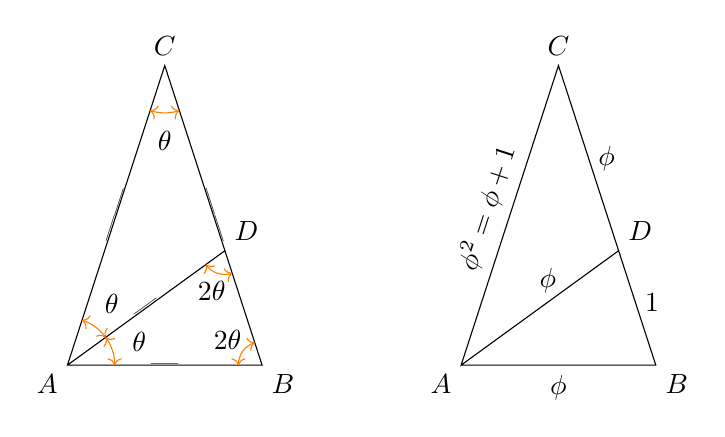
\begin{tikzpicture}[scale=1];
      \begin{scope}[shift={(0,0)}]
        \coordinate(A) at (0,0);
        \coordinate(C) at (72:4);
        \coordinate(B) at ($(C)!1!36:(A)$); %rotate A to 36 degree around C
        \tkzDefLine[bisector](C,A,B)\tkzGetPoint{D'}
        \tkzInterLL(A,D')(B,C)\tkzGetPoint{D}
        \draw(A)--(B)node[midway,sloped]{|}--(C)node[midway,sloped]{||}--cycle node[midway,sloped]{||}--(D)node[midway,sloped]{|};
        \draw pic["$\theta$",<->,draw=orange,angle eccentricity=1.6,angle radius=.6cm]{angle=D--A--C};
        \draw pic["$\theta$",<->,draw=orange,angle eccentricity=1.6,angle radius=.6cm]{angle=B--A--D};
        \draw pic["$\theta$",<->,draw=orange,angle eccentricity=1.6,angle radius=.6cm]{angle=A--C--B};
        \draw pic["$2\theta$",<->,draw=orange,angle eccentricity=1.8,angle radius=.3cm]{angle=C--B--A};
        \draw pic["$2\theta$",<->,draw=orange,angle eccentricity=1.8,angle radius=.3cm]{angle=A--D--B};
        \tkzLabelPoints[below left](A)
        \tkzLabelPoints[below right](B)
        \tkzLabelPoints[above](C)
        \tkzLabelPoints[above right](D)
      \end{scope}
      \begin{scope}[shift={(5,0)}]
        \coordinate(A) at (0,0);
        \coordinate(C) at (72:4);
        \coordinate(B) at ($(C)!1!36:(A)$); %rotate A to 36 degree around C
        \tkzDefLine[bisector](C,A,B)\tkzGetPoint{D'}
        \tkzInterLL(A,D')(B,C)\tkzGetPoint{D}
        \draw(A)--(B)node[midway,sloped,below]{$\phi$}
                --(D)node[pos=.55,right]{$1$}
                --(C)node[midway,right]{$\phi$}
                --(A)node[midway,sloped,above]{$\phi^2=\phi+1$}
                --(D)node[pos=.55,above]{$\phi$};
        \tkzLabelPoints[below left](A)
        \tkzLabelPoints[below right](B)
        \tkzLabelPoints[above](C)
        \tkzLabelPoints[above right](D)
      \end{scope}
    \end{tikzpicture}
  \end{center}
\end{definition}

\begin{theorem}
  一个等腰三角形是黄金三角形的充要条件是其顶角是$\dfrac\pi5(36^\circ)$。
\end{theorem}
\begin{proof}
  必要性:由图,$5\theta=\pi$,从而$\theta=\dfrac\pi5$。

  充分性:若等腰三角形顶角$\angle C=\dfrac\pi5$,则容易计算到到$\angle BAD=\dfrac\pi5$,从而$\triangle ABC\sim\triangle BAD$,即$\triangle ABC$是黄金三角形。
\end{proof}

\begin{question}
  证明黄金三角形各边长度的比例关系如上图所示。
\end{question}

\begin{question}
  证明正五角星(Regular Pentagram)的顶点可组成黄金三角形。
  \begin{center}
    
\begin{tikzpicture}[scale=.6]
      \coordinate(A) at ( 18:4);
      \coordinate(B) at ( 90:4);
      \coordinate(C) at (162:4);
      \coordinate(D) at (234:4);
      \coordinate(E) at (306:4);
      \draw(A)--(C)--(E)--(B)--(D)--cycle;
    \end{tikzpicture}
  \end{center}
\end{question}

\begin{example}[数值逼近]
  $\phi$是方程$x^2-x-1=0$的一个解,应用牛顿迭代法(Newton's method)逐渐逼近$\phi$。
\end{example}

选择初始点$x_0=3$,利用牛顿迭代公式
\begin{align*}
  x_{n+1}=x_n-\frac{f(x_n)}{f'(x_n)}=x_n-\frac{x_n^2-x_n-1}{2x^n-1}=\frac{x_n^2+1}{2x^n-1}
\end{align*}
从而有
\begin{align*}
  x_0&=3 &
  x_1&=2\\
  x_2&=1.66666666666667 &
  x_3&=1.61904761904762\\
  x_4&=1.61803444782168 &
  x_5&=1.61803398874999\\
  x_6&=1.61803398874989 &
  x_7&=1.61803398874989
\end{align*}
可以看出已经开始向$\phi$收敛,在上述保留14位小数的精度下迭代到$x_7$已经不变了。牛顿迭代法特别适合于应用计算机对方程进行数值求解。

\chapter{数值方法}
\label{chap:numerical-method}

数值方法通常是指应用计算机程序求解数值问题的近似解的各种方法与工具。

\section{牛顿法}
\label{sec:Newton-method}

牛顿法是一种迭代方法。迭代方法的思想是通过一个初始点,不断地迭代得到一系列的点,而这些点序列最终会收敛到目标点上。具体来说,牛顿法是通过曲线的切线来构造下一个点,因而牛顿法通常也叫做切线法。


\chapter{归纳}
\label{chap:induction}

\begin{definition}
  一个命题,若满足以下条件:
  \begin{enumerate}
  \item 存在非负整数$k_0$,命题在$n=k_0$时成立;
  \item 假设命题在$n\le k$时成立可以推出命题在$n=k+1$时成立。
  \end{enumerate}
  则该命题对任意整数$n\ge k_0$都成立。此证明方法称为数学归纳法。
\end{definition}

\begin{example}[求和]
  \begin{align*}
    \frac1{1\times2}+\frac1{2\times3}+\frac1{3\times4}+\cdots+\frac1{n\times (n+1)}
  \end{align*}
\end{example}

可以利用拆项,由$\dfrac1{k\times (k+1)}=\dfrac1k-\dfrac1{k+1}$,从而有
\begin{align*}
  &\frac1{1\times2}+\frac1{2\times3}+\frac1{3\times4}+\cdots+\frac1{(n-1)\times n}\\
  =&\left(\frac11-\frac13\right) + \left(\frac13-\frac14\right) + \cdots + \left(\frac1n-\frac1{n+1}\right)\\
  =&\frac11-\frac1{n+1}\\
  =&\frac{n}{n+1}
\end{align*}

若观察不到拆项的规律,可以考虑一下数学归纳法。记当$n=k$时的和为$S_k$,则
\begin{enumerate}
\item 当$n=1$时,有$S_1=\dfrac12$;
\item 当$n=2$时,有$S_2=\dfrac23$;
\item 当$n=3$时,有$S_3=\dfrac34$;
\item $\cdots$
\end{enumerate}
猜测,$\forall n$,有$S_n=\dfrac{n}{n+1}$。
\begin{proof}
  当$n=1$时,显然成立。

  设当$n\le k$时成立,考虑$n=k+1$的情况。
  \begin{align*}
    S_{k+1}&=S_k + \frac1{(k+1)\times(k+2)}\\
           &=\frac{k}{k+1}+\frac1{(k+1)\times(k+2)}\\
           &=\frac{k(k+2)+1}{(k+1)(k+2)}\\
           &=\frac{k^2+2k+1}{(k+1)(k+2)}\\
           &=\frac{k+1}{k+2}
  \end{align*}
  从而对任意整数$n\ge1$,猜测成立。
\end{proof}




\chapter{面积}
\label{chap:area}

\section{基本公式}
\label{sec:basic-area-formula}

% \begin{table}[htbp]
%   \centering
%   \renewcommand{\arraystretch}{1.2}
%   % The > directive lets you basically inject the contained code
%   % before each entry in that column.
%   % 
%   % The point of \arraybackslash is to return \\ to its original
%   % meaning because the \centering command alters this and could
%   % possibly give you a noalign error during compilation.
%   % \newcolumntype{C}{ >{\centering\arraybackslash} m{1cm} }
%   % \newcolumntype{D}{ >{\centering\arraybackslash} m{2cm} }
%   % \newcolumntype{E}{ >{\centering\arraybackslash} m{4cm} }
%   % \newcolumntype{F}{ >{\centering\arraybackslash} m{6cm} }

%   % define "struts", as suggested by Claudio Beccari in
%   % a piece in TeX and TUG News, Vol. 2, 1993.
%   % \newcommand\Tstrut{\rule{0pt}{2.6ex}}         % = `top' strut
%   % \newcommand\Bstrut{\rule[-0.9ex]{0pt}{0pt}}   % = `bottom' strut
  
%   \begin{tabular}{cccl}
%     \hline
%     序号&图形 & 示例 & 公式\\
%     \hline\\[2pt]
%     1 & 三角形 & \tikz{\draw(2,2)--(0,0)--(3,0)--(2,2)--(2,0)
%                             (1.8,0)--(1.8,.2)--(2,.2);
%                  \draw[|<->|](0,-.3)--(3,-.3)node[midway,fill=white]{$a$};
%                  \draw[|<->|](3.5, 0)--(3.5, 2)node[midway,fill=white]{$h$};
%                  } & $S=\frac12 ah$\\
%     2 & 矩阵 & \tikz{
%                \draw(0,0)rectangle(3,2);
%                \draw[|<->|](0,-.3)--(3,-.3)node[midway,fill=white]{$a$};
%                \draw[|<->|](3.5,0)--(3.5,2)node[midway,fill=white]{$b$};
%                } & $S=ab$\\
%     \hline
%   \end{tabular}
%   \caption{基本面积公式}
%   \label{tab:basic-area-formula}
% \end{table}

一些基本图形的面积公式列表如下:
\begin{center}
\begin{tikzpicture}
  \begin{scope}[shift={(0,0)}]
    \draw(2,2)--(0,0)--(3,0)--(2,2)--(2,0)
    (1.8,0)--(1.8,.2)--(2,.2);
    \draw[|<->|](0,-.3)--(3,-.3)node[midway,fill=white]{$a$};
    \draw[|<->|](3.5, 0)--(3.5, 2)node[midway,fill=white]{$h$};
    \node[right]at (4,1){$S=\dfrac12 ah$};
  \end{scope}

  \begin{scope}[shift={(8,0)}]
    \draw(0,0)rectangle(3,2);
    \draw[|<->|](0,-.3)--(3,-.3)node[midway,fill=white]{$a$};
    \draw[|<->|](3.5,0)--(3.5,2)node[midway,fill=white]{$b$};
    \node[right]at (4,1){$S=ab$};
  \end{scope}

  \begin{scope}[shift={(0,-4)}]
    \draw[|<->|](1,2.3)--(2.5,2.3)node[midway,fill=white]{$b$};
    \draw[|<->|](0,-.3)--(3,-.3)node[midway,fill=white]{$a$};
    \draw[|<->|](3.5,0)--(3.5,2)node[midway,fill=white]{$h$};
    \draw(0,0)--(3,0)--(2.5,2)--(1,2)--cycle;
    \node[right]at (4,1){$S=\dfrac12 (a+b)h$};
  \end{scope}

  \begin{scope}[shift={(8,-4)}]
    \draw(1.5,1)circle(1.5);
    \draw[->](1.5,1)--(3,1)node[midway,above]{$r$};
    \node[right]at(4,1){$S=\pi r^2$};
  \end{scope}

  \begin{scope}[shift={(0,-8)}]
    \draw(0,1)node(O){}--(3,1)node(A){} arc(0:30:3) node(B){}--cycle;
    \draw[|<->|](0,.6)--(3,.6)node[midway,below]{$r$};
    \draw pic["$\theta$",<->,draw=orange,angle eccentricity=1.6,angle radius=.6cm]{angle=A--O--B};
    \node[right]at(4,1.5){$S=\dfrac12 \theta r^2$};
  \end{scope}
\end{tikzpicture}
\end{center}

\begin{example}
  已知正方形边长,求阴影面积。

  \centering
  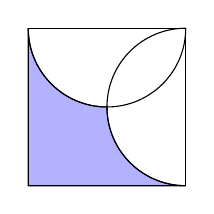
\begin{tikzpicture}[scale=2.0]
    \draw[fill=blue!30](0,0)--(1,0)arc(-90:-180:.5)arc(-90:-180:.5)--cycle;
    \draw(0,0)--(1,0)--(1,1)--(0,1)--cycle;
    \draw(1,0)arc(-90:-270:.5) (1,1)arc(0:-180:.5);
  \end{tikzpicture}
\end{example}

\hints 作辅助线,分别求各部分面积。

\begin{center}
  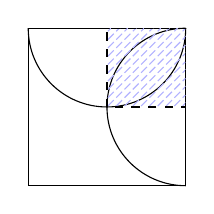
\begin{tikzpicture}[scale=2.0]
    % \draw[fill=blue!30](0,0)--(1,0)arc(-90:-180:.5)arc(-90:-180:.5)--cycle;
    \draw(0,0)--(1,0)--(1,1)--(0,1)--cycle;
    \draw(1,0)arc(-90:-270:.5) (1,1)arc(0:-180:.5);
    \draw[dashed,pattern=north east lines,pattern color=blue!30](.5,.5)rectangle(1,1);
  \end{tikzpicture}
\end{center}

\begin{example}
  求阴影面积

  \centering
  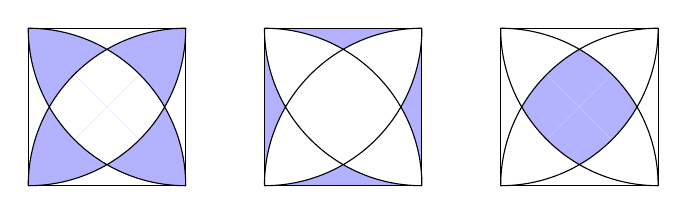
\begin{tikzpicture}[scale=1.0]
    \begin{scope}[shift={(0,0)}]
      \draw(0,0)rectangle(2,2);
      \draw[fill=blue!30,even odd rule]
           ([shift=(0:2)]0,0)arc(0:90:2)
           ([shift=(90:2)]2,0)arc(90:180:2)
           ([shift=(180:2)]2,2)arc(180:270:2)
           ([shift=(270:2)]0,2)arc(270:360:2);
    \end{scope}

    \begin{scope}[shift={(3,0)}]
      \fill[color=blue!30] (0,0)--(2,0) arc(-90:-120:2) arc(-60:-90:2);
      \fill[color=blue!30] (2,0)--(2,2) arc(0:-30:2) arc(30:0:2);
      \fill[color=blue!30] (2,2)--(0,2) arc(90:60:2) arc(120:90:2);
      \fill[color=blue!30] (0,2)--(0,0) arc(180:150:2) arc(210:180:2);
      \draw(0,0)rectangle(2,2);
      \draw([shift=(0:2)]0,0)arc(0:90:2)
           ([shift=(90:2)]2,0)arc(90:180:2)
           ([shift=(180:2)]2,2)arc(180:270:2)
           ([shift=(270:2)]0,2)arc(270:360:2);
    \end{scope}

    \begin{scope}[shift={(6,0)}]
      \fill[color=blue!30]
           ([shift=(0:2)]0,0)arc(0:90:2)
           ([shift=(90:2)]2,0)arc(90:180:2)
           ([shift=(180:2)]2,2)arc(180:270:2)
           ([shift=(270:2)]0,2)arc(270:360:2);
      \fill[color=white,even odd rule]
           ([shift=(0:2)]0,0)arc(0:90:2)
           ([shift=(90:2)]2,0)arc(90:180:2)
           ([shift=(180:2)]2,2)arc(180:270:2)
           ([shift=(270:2)]0,2)arc(270:360:2);
      \draw(0,0)rectangle(2,2);
      \draw([shift=(0:2)]0,0)arc(0:90:2)
           ([shift=(90:2)]2,0)arc(90:180:2)
           ([shift=(180:2)]2,2)arc(180:270:2)
           ([shift=(270:2)]0,2)arc(270:360:2);
    \end{scope}
  \end{tikzpicture}
\end{example}
\begin{proof}[解]
  交点将圆弧平均分成三段,每段对应于$30^\circ$的圆弧。\hints 图中三角形是等边三角形。

  \begin{center}
  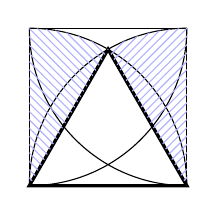
\begin{tikzpicture}[scale=1.0]
    \draw(0,0)rectangle(2,2);
    \draw([shift=(0:2)]0,0)arc(0:90:2)
         ([shift=(90:2)]2,0)arc(90:180:2)
         ([shift=(180:2)]2,2)arc(180:270:2)
         ([shift=(270:2)]0,2)arc(270:360:2);
    \coordinate (A) at (60:2);
    \draw[very thick](0,0)--(2,0)--(A)--cycle;
    \fill[pattern=north west lines,pattern color=blue!30](0,0)--(A)arc(60:90:2)--cycle;
    \fill[pattern=north east lines,pattern color=blue!30](2,0)--(2,2)arc(90:120:2)--cycle;
  \end{tikzpicture}
  \end{center}

  可按图中分割方式求解题目第二个图中阴影面积。
\end{proof}

\begin{example}
  由两个圆弧组成的图形称为半月形(lune)。求图中阴影部分半月形的面积。

  \centering
  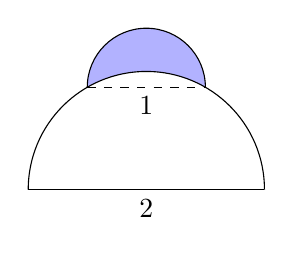
\begin{tikzpicture}[scale=1.5]
    \coordinate (O) at (0,0);
    \coordinate (A) at (120:1); 
    \coordinate (B) at (60:1);
    \coordinate (C) at ($.5*(A) + .5*(B)$);
    \draw[fill=blue!30](B)arc(0:180:.5);
    \draw[fill=white](1,0)arc(0:180:1);
    \draw[dashed](A)--(B) node[midway,below]{$1$};
    \draw(-1,0)--(1,0) node[midway, below]{$2$};;
  \end{tikzpicture}
\end{example}
\begin{proof}[提示]
  可转换为求弓形面积。

  \begin{center}
    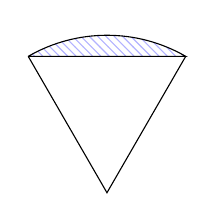
\begin{tikzpicture}[scale=2.0]
      \coordinate (O) at (0,0);
      \coordinate (A) at (120:1);
      \coordinate (B) at (60:1);
      \draw[pattern=north west lines, pattern color=blue!30](A)--(B) arc(60:120:1);
      \draw(A)--(O)--(B);
    \end{tikzpicture}
  \end{center}

  弓形面积可由上图中分割方式求出,即扇形面积减三角形面积。
\end{proof}

\begin{example}
  图中四边形为单位正方形,求阴影面积。

  \centering
  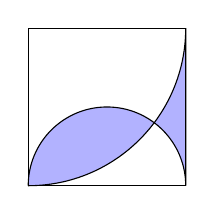
\begin{tikzpicture}[scale=1.0]
    \draw[fill=blue!30,even odd rule](0,0)arc(-90:0:2)--(2,0)arc(0:180:1);
    \draw(2,0)--(0,0)--(0,2)--(2,2);
  \end{tikzpicture}
\end{example}
\begin{proof}[解]
  除了积分,暂时未发现有其它好方法。
  \begin{align*}
    S&=\int_{x=0}^1 \left| \sqrt{0.5^2 - (x-0.5)^2} - \left(1-\sqrt{1-x^2}\right)\right| \dx\qedhere
  \end{align*}
\end{proof}

\begin{example}
  已知三角形面积为$1$,求阴影面积。其中第一个图的线段长度的比例如图所示。后两图,若其中线段长度的比例都已知,则阴影面积又该如何求解?

  \centering
  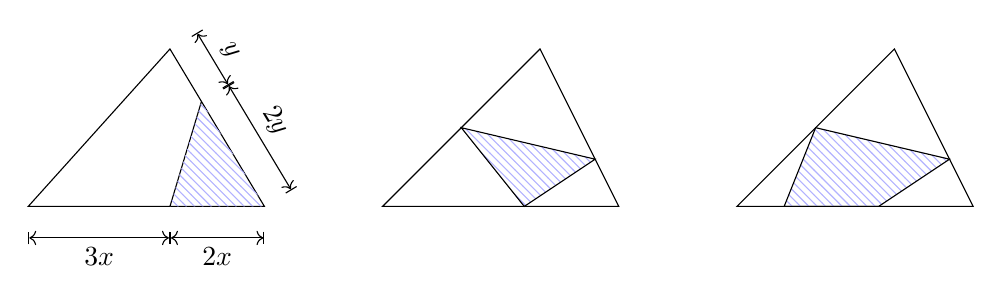
\begin{tikzpicture}[scale=1.0]
    \begin{scope}[shift={(0,0)}]
      \coordinate (A) at (1.8,2);
      \coordinate (B) at (0,0);
      \coordinate (C) at (3,0);
      \coordinate (D) at ($.6*(C)$);
      \coordinate (E) at ($2/3*(A)+1/3*(C)$);
      \draw(A)--(B)--(C)--cycle (D)--(E);
      \fill[pattern=north west lines,pattern color=blue!30](C)--(D)--(E)--cycle;

      \coordinate (B') at ($(0,-.4) + (B)$);
      \coordinate (C') at ($(0,-.4) + (C)$);
      \coordinate (D') at ($(0,-.4) + (D)$);
      \draw[|<->|](B')--(D') node[midway,below]{$3x$};
      \draw[|<->|](D')--(C') node[midway,below]{$2x$};

      \coordinate (P)  at ($({.4*2/sqrt(5.44)}, {.4*1.2/sqrt(5.44)})$);
      \coordinate (C') at ($(P) + (C)$);
      \coordinate (E') at ($(P) + (E)$);
      \coordinate (A') at ($(P) + (A)$);
      \draw[|<->|](C')--(E') node[pos=.75,above right,sloped]{$2y$};
      \draw[|<->|](E')--(A') node[pos=.75,above right,sloped]{$y$};
    \end{scope}

    \begin{scope}[shift={(4.5,0)}]
      \coordinate (B) at (0,0);
      \coordinate (C) at (3,0);
      \coordinate (A) at (2,2);
      \coordinate (D) at ($.4*(B) + .6*(C)$);
      \coordinate (E) at ($.3*(A) + .7*(C)$);
      \coordinate (F) at ($.5*(A) + .5*(B)$);
      \draw(A)--(B)--(C)--cycle;
      \draw[pattern=north west lines,pattern color=blue!30](D)--(E)--(F)--cycle;
    \end{scope}

    \begin{scope}[shift={(9,0)}]
      \coordinate (B) at (0,0);
      \coordinate (C) at (3,0);
      \coordinate (A) at (2,2);
      \coordinate (D) at ($.4*(B) + .6*(C)$);
      \coordinate (E) at ($.3*(A) + .7*(C)$);
      \coordinate (F) at ($.5*(A) + .5*(B)$);
      \coordinate (G) at ($.8*(B) + .2*(C)$);
      \draw(A)--(B)--(C)--cycle;
      \draw[pattern=north west lines,pattern color=blue!30](D)--(E)--(F)--(G)--cycle;
    \end{scope}

  \end{tikzpicture}
\end{example}
\begin{proof}[解]\mbox{}\\
  \begin{center}
    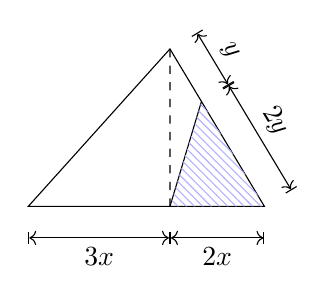
\begin{tikzpicture}[scale=1.0]
    \begin{scope}[shift={(0,0)}]
      \coordinate (A) at (1.8,2);
      \coordinate (B) at (0,0);
      \coordinate (C) at (3,0);
      \coordinate (D) at ($.6*(C)$);
      \coordinate (E) at ($2/3*(A)+1/3*(C)$);
      \draw(A)--(B)--(C)--cycle (D)--(E);
      \fill[pattern=north west lines,pattern color=blue!30](C)--(D)--(E)--cycle;

      \coordinate (B') at ($(0,-.4) + (B)$);
      \coordinate (C') at ($(0,-.4) + (C)$);
      \coordinate (D') at ($(0,-.4) + (D)$);
      \draw[|<->|](B')--(D') node[midway,below]{$3x$};
      \draw[|<->|](D')--(C') node[midway,below]{$2x$};

      \coordinate (P)  at ($({.4*2/sqrt(5.44)}, {.4*1.2/sqrt(5.44)})$);
      \coordinate (C') at ($(P) + (C)$);
      \coordinate (E') at ($(P) + (E)$);
      \coordinate (A') at ($(P) + (A)$);
      \draw[|<->|](C')--(E') node[pos=.75,above right,sloped]{$2y$};
      \draw[|<->|](E')--(A') node[pos=.75,above right,sloped]{$y$};

      \draw[dashed](A)--(D);
    \end{scope}
  \end{tikzpicture}
\end{center}

  作辅助线,可以容易看出各个三角形之间的面积关系。
\end{proof}

\section{面积法}
\label{sec:area-method}

有时解决问题可以升维或降维。比如在某些情况下求解线段问题时,可以升维成面积问题。反之,有时求解体积问题时可以降维成线段问题。

\begin{example}
  如图,$D$和$E$是$\triangle ABC$两边上一点,$O$是$AE$与$CD$的交点。若$\dfrac{CE}{BE}=\dfrac{u}{v}$,$\dfrac{AD}{BD}=\dfrac{x}{y}$,求$\dfrac{CO}{DO}$。
  \begin{center}
    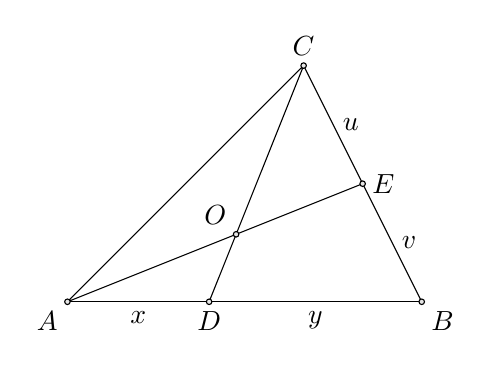
\begin{tikzpicture}[scale=1.5]
      \coordinate[label=below left:$A$](A) at (0,0);
      \coordinate[label=below right:$B$](B) at (3,0);
      \coordinate[label=above:$C$](C) at (2,2);
      \coordinate[label=below:$D$](D) at ($.6*(A)+.4*(B)$);
      \coordinate[label=right:$E$](E) at ($.5*(B)+.5*(C)$);
      \coordinate[label=above left:$O$](O) at ($2/7*(C)+5/7*(D)$);
      \draw(A)--(D) node[midway,below]{$x$};
      \draw(D)--(B) node[midway,below]{$y$};
      \draw(B)--(E) node[midway,right]{$v$};
      \draw(E)--(C) node[midway,right]{$u$};
      \draw(C)--(A)--(O)--(E) (C)--(D);
      \tkzDrawPoints(A,B,C,D,E,O)
    \end{tikzpicture}
  \end{center}
\end{example}
\begin{proof}[提示]利用面积法。如图,设$\triangle AOD$与$\triangle COE$的面积分别为$M$和$N$。
  \begin{center}
    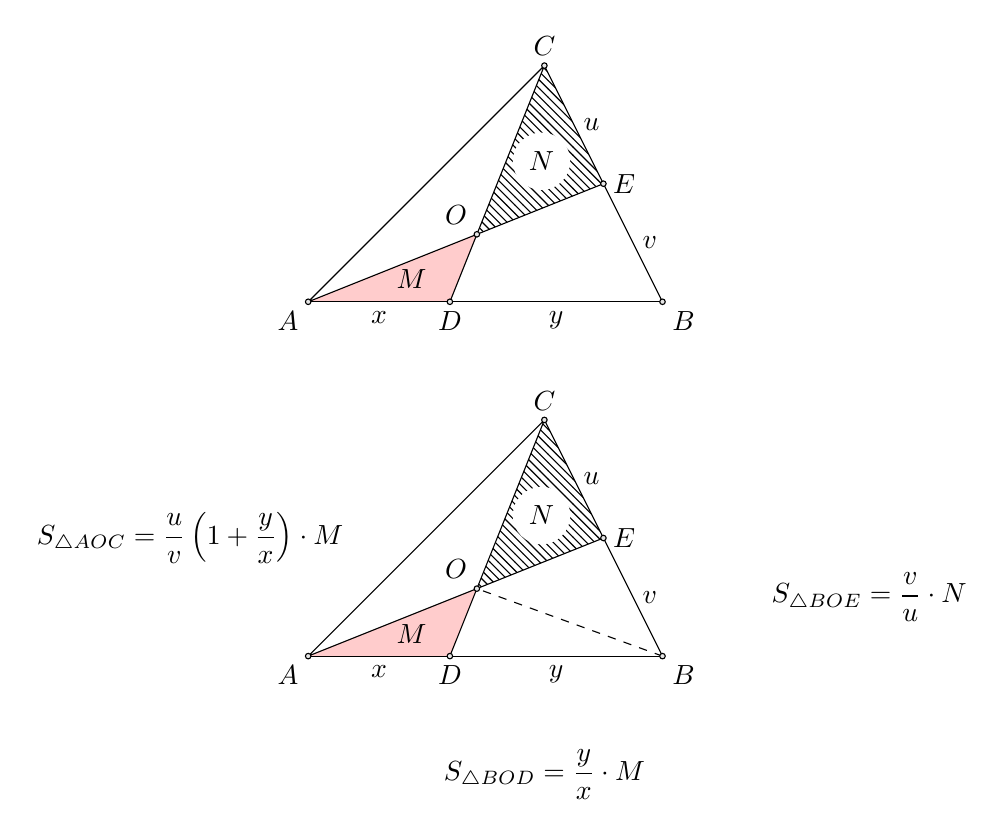
\begin{tikzpicture}[scale=1.5]
      \begin{scope}
        \coordinate[label=below left:$A$](A) at (0,0);
        \coordinate[label=below right:$B$](B) at (3,0);
        \coordinate[label=above:$C$](C) at (2,2);
        \coordinate[label=below:$D$](D) at ($.6*(A)+.4*(B)$);
        \coordinate[label=right:$E$](E) at ($.5*(B)+.5*(C)$);
        \coordinate[label=above left:$O$](O) at ($2/7*(C)+5/7*(D)$);
        \fill[color=red!20](A)--(D)--(O)--cycle;
        \fill[pattern=north west lines](C)--(E)--(O)--cycle;
        \draw(A)--(D) node[midway,below]{$x$};
        \draw(D)--(B) node[midway,below]{$y$};
        \draw(B)--(E) node[midway,right]{$v$};
        \draw(E)--(C) node[midway,right]{$u$};
        \draw(C)--(A)--(O)--(E) (C)--(D);
        \tkzDrawPoints(A,B,C,D,E,O)
        \node at ($1/3*(A)+1/3*(D)+1/3*(O)$) {$M$};
        \node[fill=white,circle] at ($1/3*(C)+1/3*(E)+1/3*(O)$) {$N$};
      \end{scope}
      \begin{scope}[shift={(0,-3)}]
        \coordinate[label=below left:$A$](A) at (0,0);
        \coordinate[label=below right:$B$](B) at (3,0);
        \coordinate[label=above:$C$](C) at (2,2);
        \coordinate[label=below:$D$](D) at ($.6*(A)+.4*(B)$);
        \coordinate[label=right:$E$](E) at ($.5*(B)+.5*(C)$);
        \coordinate[label=above left:$O$](O) at ($2/7*(C)+5/7*(D)$);
        \fill[color=red!20](A)--(D)--(O)--cycle;
        \fill[pattern=north west lines](C)--(E)--(O)--cycle;
        \draw(A)--(D) node[midway,below]{$x$};
        \draw(D)--(B) node[midway,below]{$y$};
        \draw(B)--(E) node[midway,right]{$v$};
        \draw(E)--(C) node[midway,right]{$u$};
        \draw(C)--(A)--(O)--(E) (C)--(D);
        \draw[dashed](B)--(O);
        \tkzDrawPoints(A,B,C,D,E,O)
        \node at ($1/3*(A)+1/3*(D)+1/3*(O)$) {$M$};
        \node[fill=white,circle] at ($1/3*(C)+1/3*(E)+1/3*(O)$) {$N$};
        \node(SBOE) at ($.5*(B)+.5*(E)+(2,0)$) {$S_{\triangle BOE} = \dfrac{v}{u}\cdot N$};
        \node(SBOD) at ($(B)+(-1,-1)$) {$S_{\triangle BOD}=\dfrac{y}{x}\cdot M$};
        \node(SAOC) at ($.5*(A)+.5*(C)+(-2,0)$) {$S_{\triangle AOC}=\dfrac{u}{v}\left(1+\dfrac{y}{x}\right)\cdot M$};
    \end{scope}
    \end{tikzpicture}
  \end{center}
  连接$BO$,可分别求得各部分的面积,即
  \begin{align*}
    &S_{\triangle BOD} = \frac{y}{x}\cdot M,\quad\quad
    S_{\triangle BOE} = \frac{v}{u}\cdot N\\
    \implies& S_{\triangle ABE} = \left(1 + \frac{y}{x}\right)\cdot M + \frac{v}{u}\cdot N \\
    \implies& S_{\triangle ACE} = \frac{u}{v}\cdot S_{\triangle ABE} =
              \frac{u}{v}\left(1+\frac{y}{x}\right)\cdot M + N\\
    \implies& S_{\triangle AOC} = \frac{u}{v}\left(1+\frac{y}{x}\right)\cdot M
  \end{align*}
  由此可得
  \begin{align*}
    \frac{CO}{DO}= & \frac{S_{\triangle AOC}}{S_{\triangle AOD}}= \frac{u}{v}\left(1+\frac{y}{x}\right)
  \end{align*}

  这里还可以得到关于$M$与$N$之间关系的结论。由类似的方法得到$S_{\triangle AOC}$关于$N$的表达式为
  \begin{align*}
    & S_{\triangle AOC} = \frac{x}{y}\left(1+\frac{v}{u}\right)\cdot N\\
    \implies & \frac{u}{v}\left(1+\frac{y}{x}\right)\cdot M = \frac{x}{y}\left(1+\frac{v}{u}\right)\cdot N\qedhere
  \end{align*}
\end{proof}

\begin{example}[正八边形]
  若正八边形最长的对角线为$a$,最短的对角线为$b$,则正八边形的面积是$ab$。
  \begin{center}
    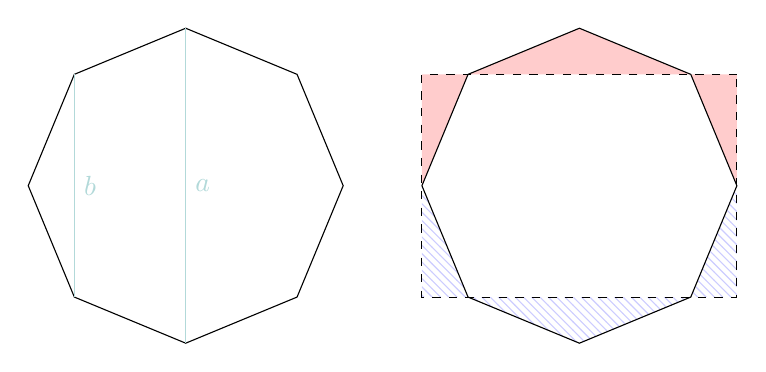
\begin{tikzpicture}[scale=1.0]
      \begin{scope}
        \foreach \i in{0,1,2,3,4,5,6,7}{%
          \coordinate(N\i) at (360/8*\i:2);
        }
        \draw(N0)--(N1)--(N2)--(N3)--(N4)--(N5)--(N6)--(N7)--cycle;
        \draw[help lines](N2)--(N6)node[midway,right]{$a$};
        \draw[help lines](N3)--(N5)node[midway,right]{$b$};
      \end{scope}
      \begin{scope}[shift={(5,0)}]
        \foreach \i in{0,1,2,3,4,5,6,7}{%
          \coordinate(N\i) at (360/8*\i:2);
        }

        \coordinate(A) at ($(N1)!(N0)!(N3)$);
        \coordinate(B) at ($(N1)!(N4)!(N3)$);
        \coordinate(C) at ($(N5)!(N4)!(N7)$);
        \coordinate(D) at ($(N5)!(N0)!(N7)$);
        % \coordinate(E) at ($(N1)!(N2)!(N3)$);
        % \coordinate(F) at ($(N5)!(N6)!(N7)$);
        \fill[red!20](N1)--(N2)--(N3);
        \fill[red!20](N0)--(A)--(N1)--cycle (N3)--(B)--(N4)--cycle;
        \fill[pattern=north west lines,pattern color=blue!20](N5)--(N6)--(N7)--cycle;
        \fill[pattern=north west lines,pattern color=blue!20](N4)--(C)--(N5)--cycle (N7)--(D)--(N0)--cycle;

        \draw[dashed](A)--(B)--(C)--(D)--cycle;
        \draw(N0)--(N1)--(N2)--(N3)--(N4)--(N5)--(N6)--(N7)--cycle;
      \end{scope}
    \end{tikzpicture}
  \end{center}

\end{example}

\chapter{二次方程}
\label{chap:quadratic-equation}

\begin{definition}[一元二次方程]
  对常数$a,b,c$及未知数$x$,以下方程称为一元二次方程
  \begin{align*}
    ax^2+bx+c=0
  \end{align*}
\end{definition}

若$a=0$,则方程退化为一元一次方程。当$a\ne0$时用配方法消去$x$的一次项可求解:
\begin{align*}
  &ax^2+bx+c=0\\
  \implies& a\cdot\left(x^2+\frac ba x + \frac{b^2}{4a^2}\right) - a\cdot\frac{b^2}{4a^2} + c = 0\\
  \implies& a\cdot\left(x+\frac{b}{2a}\right)^2=\frac{b^2-4ac}{4a}\\
  \implies& x+\frac{b}{2a} =\pm\sqrt{\frac{b^2-4ac}{4a^2}}\\
  \implies& x=-\frac{b}{2a}\pm\frac{\sqrt{b^2-4ac}}{2|a|}\\
  \implies& x=-\frac{b}{2a}\pm\frac{\sqrt{b^2-4ac}}{2a}\\
  \implies& x=\frac{-b\pm\sqrt{b^2-4ac}}{2a}
\end{align*}
即一元二次方程有实数根,当且仅当$b^2\ge4ac$,当月$b^2=4ac$时有重根。


\section{函数}
\label{sec:function}

\begin{definition}[对合,Involution]
  一个函数若存在反函数且其反函数为其本身,则称此函数为对合或对合函数。
\end{definition}

\begin{example}
  以下三个都是对合函数的例子:
  \begin{align*}
    f(x)=x,\quad g(x)=\frac1x,\quad h(x)=\frac{x}{x-1}
  \end{align*}
\end{example}

\begin{example}
  存在无限个对合函数。
\end{example}
\begin{proof}
  显然,一个函数是对合函数$\iff$其在笛卡尔坐标下的曲线关于直线$y=x$对称,这样的曲线是可以无限地构造出来。比如任意非零实数$a$,$f(x)=\frac{a}{x}$都是对合函数。或者,利用下面的定理构造。
\end{proof}

\begin{theorem}
  若$f$是对合函数,$g$有反函数$\bar g$,则$h\equiv g\circ f\circ\bar g$是对合函数。
\end{theorem}
\begin{proof}
  任意定义域内$x$,有
  \begin{align*}
    h(x)&= g(f(\bar g(x)))\\
    h(h(x))&=g(f(\underline{\bar g( g}(f(\bar g(x))) ))) = g(\underline{f(f}(\bar g(x)))) = g(\bar g(x)) = x \qedhere
  \end{align*}
\end{proof}

\chapter{对称性}
\label{chap:symetric}

\begin{example}
  求解方程 $x^4+x^3+x^2+x+1=0$。
\end{example}
\begin{proof}[解]
  利用系数的对称性及$x\ne 0$,两边除以$x^2$,有
  \begin{align*}
    &x^2+x+1+\frac1x+\frac1{x^2}=0\\
    \implies& \left(x^2+\frac1{x^2}\right) + \left(x+\frac1x\right) + 1 = 0
  \end{align*}
  分组后令$u=x+\dfrac1x$,则有$u^2=x^2+\dfrac1{x^2}+2$,从而原方程变换为
  \begin{align*}
    u^2 + u - 1 = 0
  \end{align*}
  剩余略。
\end{proof}


\chapter{极端原理}
\label{chap:extreme}



\chapter{无穷级数}
\label{chap:inifinite-series}

\begin{example}[等比数列]
  求无穷等比数列的和,其中比例系数$q<1$:
  \begin{align*}
    S=a + aq + aq^2 + aq^3 + \cdots
  \end{align*}
\end{example}
\begin{proof}[解]
  两边同乘以$q$,有
  \begin{eqnarray*}
            & qS=& aq + aq^2 + aq^3 + aq^4 + \cdots\\
    \implies& qS=& S - a\\
    \implies&  S=& \frac{a}{1-q}
  \end{eqnarray*}
  关于无穷级数的一个技巧在于乘以其个数后找到与原数的关系。
\end{proof}

\begin{example}[$\zeta$函数]
  $\zeta$函数是按以下无穷级数定义的函数
  \begin{align}
    \zeta(x)\equiv \frac1{1^x} + \frac1{2^x} + \frac1{3^x} + \cdots
  \end{align}
  当$x=1$时,$\zeta(1)$就是调和函数。证明当$x\ge2$时,$\zeta$函数是收敛的。
\end{example}
\begin{proof}
  显然$\zeta(x)$在$x>1$时是严格单调递减正函数,从而只需考虑$\zeta(2)$的收敛性。由
  \begin{align*}
    \frac1{k^2} \le \frac1{k(k-1)},\quad\forall k>1
  \end{align*}
  从而有$\zeta(2)$的前$n$项和为
  \begin{align*}
    \zeta(2)_n&=\frac1{1^2} + \frac1{2^2} + \frac1{3^2} + \cdots + \frac1{n^2}\\
            &\le \frac1{1^2} + \frac1{2\times(2-1)} + \frac1{3\times(3-1)} +\frac1{4\times(4-1)}+ \cdots + \frac1{n\times(n-1)}\\
            &= 1 + \left(1 - \frac12\right) + \left(\frac12 - \frac13\right) + \cdots + \left(\frac1{n-1}-\frac1n\right)\\
            &= 2 - \frac1n
  \end{align*}
  令$n\to+\infty$,有$\zeta(2)\le2$。从而$\zeta(2)$有上界,收敛。
\end{proof}

\begin{example}
  求下列级数的和:
  \begin{align*}
    q + 2q^2 + 3q^3 + 4q^4 + \cdots + nq^n
  \end{align*}
\end{example}
\begin{proof}[提示]
  记其和为$S_n$,则
  \begin{align*}
    qS_n = q^2 + 2q^3 + 3q^4 + 4q^5 + \cdots + nq^{n+1}
  \end{align*}
  与原式相减,则有
  \begin{align*}
    S_n - qS_n = \underline{q + q^2 + q^3 + \cdots + q^n} - nq^{n+1}
  \end{align*}
  去掉首尾两项(下划线部分)后是等比级数,应用等比数列求和公式并化简可得。
\end{proof}

\begin{example}
  求和
  \begin{align*}
    \dfrac1{1\times2\times3} + \dfrac1{2\times3\times4} + \dfrac1{3\times4\times5} + \cdots + \dfrac1{n\times(n+1)\times(n+2)}
  \end{align*}
\end{example}
\begin{proof}[提示]
  利用下式拆项
  \begin{align*}
    \frac1{n(n+1)(n+2)} = \frac12 \left(\frac1{n(n+1)} - \frac1{(n+1)(n+2)}\right)&\qedhere
  \end{align*}
\end{proof}

\begin{example}[推广]
  是否有简单方法对下式求和
  \begin{align*}
    S_{n,k}=\sum_{i=1}^{n} \frac1{\prod_{j=i}^{i+k-1} j}
  \end{align*}
  如
  \begin{align*}
    S_{n,4} = \sum_{i=1}^{n}\frac1{i(i+1)(i+2)(i+3)}
  \end{align*}
\end{example}

\begin{example}
  对下式求和:
  \begin{align*}
    1\times2\times3 + 2\times3\times4 + 3\times4\times5 + \cdots + n(n+1)(n+2)
  \end{align*}
  并推广。
\end{example}

\begin{example}
  计算可知$\left\lfloor\sqrt{44}\right\rfloor=6$,$\left\lfloor\sqrt{4444}\right\rfloor=66$,其中$\left\lfloor x\right\rfloor$是指对$x$向下取整。请推广。
\end{example}
\begin{proof}[解]
  记
  \begin{align*}
    S_1&=44\\
    S_2&=4444=100S_1+44\\
    S_3&=444444=100S_2+44\\
    \multicolumn{2}{c}{$\cdots$}\\
    S_n&=100S_{n-1}+44
  \end{align*}
  其中$6<\sqrt{S_1}<7$,假设对任意$n\le k$,有
  \begin{align*}
    10*b_n+6<S_n<10*b_n+7
  \end{align*}
  其中$b_n=6*10^0+6*10+6*10^2+\cdots+6*10^n$,
\end{proof}

\begin{example}
  求和$1\times 1!+2\times 2! + \cdots + n\times n!.$
\end{example}
\begin{proof}[解]
  记其和为$S_n$,即
  \begin{align*}
    S_n&=1\times 1!+2\times 2! + \cdots + n\times n!
  \end{align*}
  则
  \begin{align*}
    S_n - S_{n-1} = n\times n!
  \end{align*}

\end{proof}


\section{单调函数}
\label{sec:monotonic-functions}

\begin{example}
  任意非负数$a,b,c$满足$a\le b+c$,则
  \begin{align*}
    \frac{a}{1+a}\le \frac{b}{1+b} + \frac{c}{1+c}
  \end{align*}
  并说明等号成立的充要条件。
\end{example}

\begin{proof}
  容易知道$f(x)=\dfrac{x}{1+x}$在$x\ge0$时是严格单调递增函数,从而
  \begin{align*}
    \frac{a}{1+a}&\le\frac{b+c}{1+b+c}&\text{等号成立}\iff a=b+c\\
    &=\frac{b}{1+b+c} + \frac{c}{1+b+c}\\
    &\le\frac{b}{1+b} + \frac{c}{1+c}&\text{等号成立}\iff b=c=0
  \end{align*}
  从而原不等式得证,且当且仅当$a=b=c=0$时等号成立。
\end{proof}

\chapter{度量空间}
\label{chap:metric-space}

容易知道,对$\forall x,y,z$,欧氏空间中的距离满足以下性质:
\begin{enumerate}
\item 非负性。即$d(x,y)\ge0.$
\item {\color{red}同一性?}。即$d(x,y)=0\iff x=y.$
\item 对称性。即$d(x,y)=d(y,x).$
\item 三角不等式。即$d(x,y)\le d(x,z)+d(z,y).$
\end{enumerate}

上面的非负性可以由其余三条性质推出(请自行推导)。任意空间中二元函数若满足上述的{\color{red}同一性?}、对称性及三角不等式,则称其为欧氏空间中的一个度量,也称为距离。点集配上度量,就是一个度量空间。

\begin{definition}[度量空间,Metric Space]
  点集$\mathcal{S}$,$d$是$\mathcal{S}$上的一个度量,则称$(\mathcal{S},d)$为一个度量空间。
\end{definition}

\begin{definition}[柯西序列,Cauchy Sequence]
  序列$x_1,x_2,x_3,\cdots$,若对任意正数$\epsilon$,存在正整数$N_\epsilon$,使得$\forall m,n>N_\epsilon$,有$d(x_m,x_n)<\epsilon$,则称此序列是度量$d$下的柯西序列。
\end{definition}

柯西序列是越到后面越密集的序列。若柯西序列在$\mathcal{S}$收敛,则其收敛点是唯一的(请自行推导。\hints 反证)。

\begin{definition}[完备性]
  若一个度量空间中的任意柯西序列都收敛于空间中某一个点,则称此度量空间是完备的。
\end{definition}

\begin{example}[有理数集]
  证明有理数集在普通实数距离下不是完备的。
\end{example}
\begin{proof}[解释]
  在实数轴上,有理数集是有“洞”的,而填充这些洞的就是无理数。用有理数构造一个柯西序列,使其收敛于某个无理数,即可得证。比如可以利用$\phi$的连分数表示来构造,即
  \begin{align*}
    x_1=1,\quad x2=1+\frac1{x_1},\quad x_3=1+\frac1{x_2},\cdots &\qedhere
  \end{align*}
\end{proof}


\chapter{不动点}
\label{chap:fixed-point}

本节内容需要拓扑与泛函分析的知识,不需深究。

\begin{example}
  两张内容一样的地图,把小地图放在大地图上,使小地图完全在大地图内,则必有一点,使两张地图上对应的点代表同一个物理位置。
\end{example}

此问题也有另外一种描述方式:把一张地图放在地上,则地图上必有一点正好在它所代表的物理位置的正上方。在这种描述里,大地图对应于所在城市/国家/甚至地球,小地图则对应于地上的地图。

要回答这问题,需要用到\term{不动点}理论。点$x$称为是映射$f$的不动点,若$f(x)=x$,即对不动点映射过后的像不动,还是落在自身。不动点定理表明在某些条件下,映射至少有一个不动点。

\begin{definition}[压缩映射]
  距离空间$\mathcal{D}$上的映射$f:\mathcal{D}\to\mathcal{D}$称为是压缩映射,若存在$q\in[0,1)$,使得任意$x,y$有
  \begin{align}
    d(f(x),f(y))\le q d(x,y)
  \end{align}
\end{definition}

\begin{theorem}[巴拿赫不动点定理,压缩不动点定理,Banach fixed-point theorem]
  完备距离空间上压缩映射存在唯一的不动点$x^*$,且由任意一点$x_0$通过以下迭代:
  \begin{align*}
    x_{n}=f(x_{n-1}),\quad\quad n=1,2,3,\cdots
  \end{align*}
  有$x_n\to x^*$。
\end{theorem}
\begin{proof}
  需要用到拓扑与泛函分析的知识,此处略过。
\end{proof}

回到大小地图的问题,在大小地图所在平面上建立坐标系,考虑将大地图上的点对应的坐标$x$映射到小地图上的点对应的坐标$x'$的映射$f$,其中$x$与$x'$在大小地图上表示同一个物理位置,则容易知道$f$是一个压缩映射,因为每两个点的距离都被压缩了。从而由巴拿赫定理,存在唯一的不动点。

\chapter{恒等式}
\label{chap:identities}

\section{基本恒等式}
\label{sec:basic-identities}

\begin{example}[两数和的幂]$\forall a,b\in\mathcal{R}$,有
  \begin{align*}
    (a + b)^2 &= a^2 + 2ab + b^2\\
    (a + b)^3 &= a^3 + 3a^2b + 3ab^2 + b^3\\
    (a + b)^4 &= a^4 + 4a^3b + 6a^2b^2 + 4ab^3 + b^4
  \end{align*}
\end{example}
对于$(a-b)^2$及$(a-b)^3$这种,只要在上式中把$b$换为$-b$即可。观察上述$(a+b)^n$的系数,可以发现其与下面的杨辉三角是一致的:
\begin{center}
  \begin{tikzpicture}[scale=1.0]
    \begin{scope}[shift={(.5,1)}]
      \foreach \x/\v in {1/1,2/1}{%
        \node at (\x,0) {\v};
      }
    \end{scope}
    \begin{scope}[shift={(0,0)}]
      \foreach \x/\v in {1/1,2/2,3/1}{%
        \node at (\x,0) {\v};
      }
    \end{scope}
    \begin{scope}[shift={(-.5,-1)}]
      \foreach \x/\v in {1/1,2/3,3/3,4/1}{%
        \node at (\x,0) {\v};
      }
    \end{scope}
    \begin{scope}[shift={(-1,-2)}]
      \foreach \x/\v in {1/1,2/4,3/6,4/4,5/1}{%
        \node at (\x,0) {\v};
      }
    \end{scope}
    \begin{scope}[shift={(-1.5,-3)}]
      \foreach \x/\v in {1/1,2/5,3/10,4/10,5/5,6/1}{%
        \node at (\x,0) {\v};
      }
    \end{scope}
    \foreach \y in{1,2,3,4,5}{%
      \node[left] at (-2,2-\y){$n=\y$};
    }
  \end{tikzpicture}
\end{center}


\begin{example}[配方]$\forall a\ne 0$,有
  \begin{align*}
    ax^2 + bx + c = a\left(x-\frac{b}{2a}\right)^2 + \frac{4ac - b^2}{4a}
  \end{align*}
\end{example}

\section{代数}
\label{sec:algebra-identities}

\begin{theorem}[Sophie-Germain恒等式]
  $\forall x,y$,有
  \begin{align*}
    x^4 + 4y^4 = (x^2 + 2xy + 2y^2)(x^2 - 2xy + 2y^2)
  \end{align*}
\end{theorem}
在上式中令$x=1$,可以得到哥德巴赫定理;令$y=1$,则可以得到吉梅茵定理。
\begin{theorem}[哥德巴赫定理,Goldbach Theorem]\mbox{}\par
  对任意整数$n>1$,$4n^4+1=(1+2n+2n^2)(1-2n+2n^2)$是合数。  
\end{theorem}
\begin{theorem}[吉梅茵定理,Germain Theorem]\mbox{}\par
  任意整数$n>1$,$n^4+4=(n^2+2n+2)(n^2-2n+2)$是合数。
\end{theorem}


\begin{theorem}[贝祖定理,B\'ezout's identity]\label{th:Bezout}
  $\forall a,b\in\mathcal{Z},\exists x,y\in\mathcal{Z}$使得
  \begin{align*}
    ax+by=\mathrm{gcd}(a,b)
  \end{align*}
  若$a,b$互质,则有$ax+by=1$。
\end{theorem}

\begin{theorem}\label{th:inverse-bezout}
  若整数$x,y,a,b$满足$ax+by=1$,则$x,y$互质。从而$\gcd(a,b)=\gcd(a,y)=\gcd(x,b)=\gcd(x,y)=1$。
\end{theorem}
\begin{proof}
  记$g=\gcd(x,y)$,则$x'=x/g$与$y'=y/g$是互质的两个整数,代入有
  \begin{align*}
    1=ax+by=ax'g+by'g=g(ax'+by')
  \end{align*}
  从而$g\mid 1\implies g=1$。
\end{proof}

%%% $x,y$称为$(a,b)$的B\'ezout系数。一般来说,$(a,b)$的B\'ezout系数$x,y$不是唯一的,可以通过扩展欧几里得算法来计算得到。
$x,y$称为$(a,b)$的B\'ezout系数。一般来说,$(a,b)$的B\'ezout系数$x,y$不是唯一的,可以通过类似于欧几里得辗转相除法得到。

\begin{example}
  求整数$a,b$使得$211a+37b=1$。
\end{example}
\begin{proof}[提示]
\begin{align*}
  211a+37b=1 &\iff 37b=1-211a \\
             &\iff b=\frac{1-211a}{37}=-5a+\frac{1-26a}{37}\\
             &\iff b=-6a+\frac{1+11a}{37} 
\end{align*}
令$1+11a=37t_1$,其中$t_1$为整数,从而
\begin{align*}
  1+11a=37t_1 & \iff a=\frac{37t_1-1}{11}=3t_1 + \frac{4t_1-1}{11}
\end{align*}
令$4t_1-1=11t_2$,其中$t_2$为整数,则$t_1=2t_2+(3t_2+1)/4$。若能观察出来取$t_2=1$可使$t_1$为整数,则代入即可。

若观察不出来,继续令$3t_2+1=4t_3$,则$t_2=t_3+(t_3-1)/3$,若还观察不出来$t_3$应取什么值可使$t_2$为整数,继续令$t_3-1=3t_4$,从而$t_3=3t_4+1$,整数$t_4$可随意挑选,再一步步反向代入,可得$t_3,t_2,t_1,a,b$。
\end{proof}


% \begin{definition}[扩展欧几里得算法]
%   Ref. \verb|https://en.wikipedia.org/wiki/Extended_Euclidean_algorithm|
% \end{definition}

\begin{example}[1959 IMO]
  求证对任意正整数$n$,分数$\dfrac{21n+4}{14n+3}$不可约。
\end{example}
\begin{proof}[提示]
  相当于证明$21n+4$与$14n+3$互质。尝试使用定理\ref{th:inverse-bezout},若能找到两个整数$a,b$,使得$a(21n+4)+b(14n+3)=1$,则有$21n+4$与$14n+3$互质。而
  \begin{align*}
    a(21n+4)+b(14n+3)=1 \iff (21a + 14b)n + 4a + 3b = 1
  \end{align*}
  而上式要对任意整数$n$成立,等价于以下两式同时成立
  \begin{align*}
    21a+14b=0, \quad 4a+3b=1
  \end{align*}
  而这个方程组是有整数解$a=-2, b=3$,从而原问题得证。
\end{proof}

\begin{example}\label{ex:sum-is-negative-to-product}
  对任意满足$a+b\ne0$,$b+c\ne0$,$c+a\ne0$的实数$a,b,c$,则以下三个数的和与积互为相反数:
  \begin{align*}
    \frac{a-b}{a+b},\quad \frac{b-c}{b+c},\quad \frac{c-a}{c+a}
  \end{align*}
  即
  \begin{align*}
    \frac{a-b}{a+b} + \frac{b-c}{b+c} + \frac{c-a}{c+a} 
    + \frac{a-b}{a+b} \cdot \frac{b-c}{b+c} \cdot \frac{c-a}{c+a} = 0
  \end{align*}
\end{example}
\begin{proof}
  引入几个记号:
  \begin{align*}
    S_{l}\equiv&\, \frac{a-b}{a+b} + \frac{b-c}{b+c} + \frac{c-a}{c+a} \\
    S_{r}\equiv&\,\frac{a-b}{a+b} \cdot \frac{b-c}{b+c} \cdot \frac{c-a}{c+a}\\
    P\equiv&\,S_{r}\cdot (a+b)(b+c)(c+a) = (a-b)(b-c)(c-a)
  \end{align*}
  则问题中的等式等价于
  \begin{align*}
    S_{l}\cdot (a+b)(b+c)(c+a) + P = 0
  \end{align*}
  最直接的方法,是逐项展开,合并同类项。
  \begin{align*}
     &\, S_{l}\cdot (a+b)(b+c)(c+a)\\
    =&\, (a-b)(b+c)(c+a) + (b-c)(c+a)(a+b) + (c-a)(a+b)(b+c)\\
    =&\, (c+a)\left( (a-b)(b+c) + (b-c)(a+b) \right) + (c-a)(a+b)(b+c)\\
    =&\, 2b(c+a)(a-c) + (c-a)(a+b)(b+c)\\
    =&\, (a-c)(2bc+2ab - (ab+ac+bb+bc))\\
    =&\, (a-c)(bc+ab - ac-bb)\\
    =&\, (a-c)(c(b-a)+b(a-b))\\
    =&\, (a-c)(b-a)(c-b)\\
    =&\, -(a-b)(b-c)(c-a) = -P&&\qedhere
  \end{align*}
\end{proof}

\begin{example}
  若$a=3,b=4,c=5$,则
  \begin{align*}
    \frac{a-b}{a+b} = \frac{3-4}{3+4} = -\frac17\\
    \frac{b-c}{b+c} = \frac{4-5}{4+5} = -\frac19\\
    \frac{c-a}{c+a} = \frac{5-3}{5+3} = \phantom{-}\frac14
  \end{align*}
  其和为
  \begin{align*}
    -\frac17 - \frac19 + \frac14 = \frac{-9\times4 - 7\times4 + 7\times9}{4\times7\times9} = -\frac1{4\times7\times9}
  \end{align*}
  容易看出,其和为其积的相反数。
\end{example}

\section{重要恒等式}
\label{sec:important-identities}

以下几个恒等式不常见,却是竞赛中的常客。虽无需记忆,但可以留点印象,知道有这么回事,对解题有大帮助。

\begin{example}\label{ex:product-of-four-continuous-integer}
  证明对任意$x\in\mathcal{R}$,有
  \begin{align*}
    x(x+1)(x+2)(x+3)+1=\left( x^2+3x+1\right )^2
  \end{align*}
\end{example}
展开两边可得。换一个形式,则有
\begin{align*}
  \sqrt{x(x+1)(x+2)(x+3)+1}= x^2+3x+1 = (x + 1)^2 + x
\end{align*}


\begin{example}
  求$\sqrt{2019\times2020\times2021\times2022+1}-2020^2$。

  在恒等式$\sqrt{x(x+1)(x+2)(x+3)+1}= x^2+3x+1 = (x + 1)^2 + x$中令$x=2019$,则有
  $\sqrt{2019\times2020\times2021\times2022+1}-2020^2=2019$。
\end{example}

\begin{theorem}[Fibonacci Identity]任意实数$a,b,c,d$,有恒等式
  \begin{align*}
    \left(a^2+b^2\right)\left(c^2+d^2\right)
    = \left(ac +  bd\right)^2 + \left(ad -  bc\right)^2
    = \left(ac -  bd\right)^2 + \left(ad +  bc\right)^2 
  \end{align*}
\end{theorem}


\begin{theorem}
  若$\alpha, \beta, \gamma$均非$\pi/2$的奇数倍,则等式
  \begin{align*}
    \tan\alpha +\tan\beta+\tan\gamma=\tan\alpha \cdot \tan\beta \cdot \tan\gamma
  \end{align*}
  当且仅当$\alpha+\beta+\gamma$是$\pi$的整数倍时成立。
\end{theorem}

\section{完全平方数}
\label{sec:perfect-squares}

\begin{example}[1953 \kurschak]
  $\forall n\in\mathcal{Z}^+$,若正整数$d$整除$2n^2$,则$n^2+d$不是完全平方数。
\end{example}

\hints 反证。令$d=2n^2/k$,若$n^2+d=n^2+2n^2/k=m^2$,则$(mk)^2=n^2(k^2+2k)$,从而$k^2+2k$也是一个完全平方数。然而$k^2<k^2+2k<k^2+2k+1=(k+1)^2$,即$k^2+2k$位于两个相邻的完全平方数之间,从而不能是完全平方数,矛盾。

\chapter{抽屉原理}
\label{chap:pigeonhole-principle}

\section{原理}
\label{sec:pigeonhole-principle-theory}

\begin{theorem}[抽屉原理,鸽笼原理,鸽巢原理,Pigeonhole principle]
  若有$n$个笼子和$kn+1$只鸽子,所有的鸽子都被关在鸽笼里,那么至少有一个笼子有至少$k+1$只鸽子。
\end{theorem}

\begin{proof}
  反证法,若每个笼子最多有不超过$k$个鸽子,那么所有笼子鸽子总数不超过$kn$个,与原来有$kn+1$个鸽子矛盾。
\end{proof}

当$k=1$时,是抽屉原理最直观的情况:若有$n$个笼子和$n+1$只鸽子,所有的鸽子都被关在鸽笼里,那么至少有一个笼子有至少$2$只鸽子,即装有不少于两个鸽子的笼子数最少是$1$。

\think 若上面$n+1$只鸽子换成$n+1,n+2,\cdots$是否成立?对于$2n-1$、$2n$及$2n+1$只鸽子,又可以得到什么样的结论?

\begin{example}
  普遍认为成人的头发数量约在10万左右,那么对于深圳的常住人口(按2018年2180万算),基本可以肯定有人有相同的头发数。
\end{example}

\begin{proof}
  按头发数做鸽笼,按统计数据成人头发平均约为10万左右,假设大部分深圳常住人口(比如2180万的80\%>1600万)的头发数量都小于等于1000万根。按抽屉原理可得。
\end{proof}

\begin{example}
  在$1,2,\cdots,100$里任意选51个数,总能在这选出来的数中找到两个互质数。
\end{example}

\begin{proof}
  将100个数按$(1,2), (3,4), \cdots, (99,100)$分为50组,则选51个数总有两个落到同一组中,而同一组的两数互质,从而得证。
\end{proof}

\begin{question}
  在$1,2,\cdots,100$里任意选51个数,总能在这选出来的数中找到两个,使得其中一个被另一个整除。
\end{question}
\hints $\forall a\in\mathcal{Z}^+$,存在奇数$k$及整数$n$,使得$a=k\cdot 2^n$。对所有整数按$k$分类。

\begin{example}
  在任意9个两两不等的实数中,总能选出两个,设其为$a,b$,满足以下条件
  \begin{align*}
    0 < \frac{a-b}{1+ab} < \sqrt2 -1
  \end{align*}
\end{example}

\begin{proof}[提示]
  联想公式
  \begin{align*}
    \tan(\alpha-\beta)=\frac{\tan\alpha-\tan\beta}{1+\tan\alpha\tan\beta}
  \end{align*}

  而$\tan(x)$的周期是$(-\pi/2, \pi/2]$,将区间8等份(让9个数总有两个落入其中一份)为以下8个区间
  \begin{align*}
    (-\frac\pi2, -\frac{3\pi}8], (-\frac{3\pi}8, -\frac\pi4], \cdots, (\frac{3\pi}8, \frac\pi2]
  \end{align*}

  $\forall a, \exists\hat a\in(-\pi/2, \pi/2], s.t. \tan\hat a = a$,从而任意9个实数,总存在两个,记为$a,b$,存在$\hat a, \hat b$落在上述8个区间中的同一个,且有$a=\tan\hat a, b=\tan\hat b$。不妨设$a>b$,从而$0<\hat a-\hat b<\pi/8$,由$\tan(x)$在上述每个区间中均为严格单调递增,有
  \begin{align*}
             & 0 < \tan(\hat a - \hat b) < \tan\frac\pi8\\
    \implies & 0 < \frac{a - b}{1+ab} < \sqrt2 - 1&\qedhere
  \end{align*}
\end{proof}


\begin{question}[XLI Mathematical Olympiad in Poland]
  一个三角形可以放置在一个单位正方形内,且存在一种放置方法使得正方形的中心不在三角形内。那么该三角形有一条边长小于1。
\end{question}

\hints 将正方形划分几份,使得三角形至少有两个顶点落在某份中。

%%%%%%%%%%%%%%%%%%%%
%%% Questions
%%%%%%%%%%%%%%%%%%%%
\begin{question}
  从$1,2,\cdots,100$中任意取11个数字,那么这11个数字组成的集合中,总存在两个不相交的非空子集,其元素之和相等。
\end{question}
\begin{proof}[提示}
11个元素组成的集合,其非空真子集总共有$2^{11}-2=2046$个。
% 其中两两互补,即任意一个总有能找到一个与之互补。从而将11个元素分成两份且每份都至少有一个元素的方法共有$2046\div2=1023$个
而1到100取10个数字(\think 为什么取10个而不是11个?取11个其和已经最大了,没有真子集的和能与其相比了。),其和最大值为$91+92+\cdots+100=955$。从而由抽屉原理,这2045个子集中,总有两个的和是相等的,且显然这两个和相等的子集,没有一个是另一个的真子集(否则其和就不相等了),在这两个子集中去掉相同的元素,就可以得到两个不相交、非空且和相等的集合。
\end{proof}

\begin{question}
  在三维空间中任意选取9个坐标都是整数的点。证明这连接9个点而形成的线段中至少包含另外一个坐标为整数的点
\end{question}

\begin{question}
  任意六个人中,以下两个结论总有一个成立:
  \begin{enumerate}
  \item 其中有三人互相认识。
  \item 其中有三人互相不认识。
  \end{enumerate}
\end{question}

\hints 相当于正六边形的六个顶点用两种颜色的线段两两连接起来,则这些线段组合的三角形中,总存在一个同色的三角形。

\begin{question}
  任意一个16位的正整数的数字所组成的数字串中,总存在一个子串,其数字的乘积是一个完全平方数。
\end{question}

\hints 若16位数中含有数字$0,1,4,9$,那么取这个数字本身组成的子串即可,从而只需考虑由数字$2,3,5,6,7,8$组成的16位数。由于
\begin{align*}
  6 = 2\times 3,\quad 8=2^3
\end{align*}
从而任意一个子串各数字的乘积可以写成如下形式
\begin{align*}
  2^a \times 3^b \times 5^c \times 7^d
\end{align*}
若$a,b,c,d$都是偶数,那么这个子串数字的乘积就是完全平方数。而$a,b,c,d$的奇偶组合数总共有$2^4=16$种,即
\begin{align*}
  \text{(奇奇奇奇)},\quad \text{(奇奇奇偶)},\quad \text{(奇奇偶奇)},\quad \text{(奇奇偶偶)}\\
  \text{(奇偶奇奇)},\quad \text{(奇偶奇偶)},\quad \text{(奇偶偶奇)},\quad \text{(奇偶偶偶)}\\
  \text{(偶奇奇奇)},\quad \text{(偶奇奇偶)},\quad \text{(偶奇偶奇)},\quad \text{(偶奇偶偶)}\\
  \text{(偶偶奇奇)},\quad \text{(偶偶奇偶)},\quad \text{(偶偶偶奇)},\quad \text{(偶偶偶偶)}
\end{align*}

从而至少需要构造17种选取方式。记16位数各数字按顺序分别为$x_1,x_2,\cdots,x_{16}$,令
\begin{align*}
  F(k) =
  \begin{cases}
    1 = 2^0 \times 3^0 \times 5^0 \times 7^0 & k=0\\
    \prod_{i=1}^k x_i = 2^{a_k} \times 3^{b_k} \times 5^{c_k} \times 7^{d_k},&k=1,2,\cdots,16
  \end{cases}
\end{align*}
则$F(0),F(1),\cdots,F(16)$这17个数中至少有两个,其$a,b,c,d$的奇偶性组合相同,不妨记为$F(k_1),F(k_2)$,且$k_1<k_2$,从而$F(k_2)/F(k_1)$是完全平方数,从而两个数对应的子串,长串中拿掉短串部分,其数字乘积即为完全平方数。


\chapter{Buffalo Way}
\label{chap:buffalo-way}

Buffalo Way(BW)是一种方法,通常用于解决对称性问题,对于$x_1\le x_2\le x_3\le \cdots\le x_n$,令
\begin{align*}
  x_1&=y_1\\
  x_2&=y_1+y_2\\
  x_3&=y_1+y_2+y_3\\
  \cdots&\cdots\\
  x_n&=y_1+y_2+y_3+\cdots+y_n
\end{align*}
其中除$y_1$外$y_2,y_3,\cdots y_n$均为非负数。代入原问题换元求解。

\begin{example}
  证明:若$0\le a\le b\le c$,则$(a+b)(a+c)^2\ge 6abc$。
\end{example}
\begin{proof}
  应用Buffalo Way,令$a=x$, $b=x+y$, $c=x+y+z$,其中$x$,$y$,$z$均为非负数。代入,有
  \begin{align*}
    &(a+b)(a+c)^2\ge 6abc\\
    \iff& (2x+y)(2x+y+z)^2\ge 6x(x+y)(x+y+z)
  \end{align*}
  化简后上式等价于
  \begin{align*}
    2x^3+2x^2z+2xyz+2xz^2+y^3+2y^2z+yz^2\ge 0
  \end{align*}
  由于$x,y,z$非负,上式显然成立,且等号成立时当且仅当以下各式同时满足
  \begin{align*}
    2x^3&=0,    &2x^2z&=0,  &2xyz&=0,  &2xz^2&=0\\
    y^3&=0,     &2y^2z&=0,  &yz^2&=0   &     &
  \end{align*}
  即$x=y=0$,$z$任意。即等号成立当且仅当$a=b=0$。
\end{proof}

\begin{example}
  证明:对于正数$x,y,z$,有
  \begin{align*}
    \sum_{\mathrm{cyc}} \frac{x^4}{8x^3+5y^3}\ge\frac{x+y+z}{13}
  \end{align*}
  其中$\sum\limits{\mathrm{cyc}}$表示轮换求和,对上式的$x$,$y$和$z$作轮换,则有
  \begin{align*}
    \sum_{\mathrm{cyc}}\frac{x^4}{8x^3+5y^3} \implies
    \begin{cases}
      \dfrac{x^4}{8x^3+5y^3} \xRightarrow{x\leftarrow x, y\leftarrow y} \dfrac{x^4}{8x^3+5y^3} \\
      \dfrac{x^4}{8x^3+5y^3} \xRightarrow{x\leftarrow y, y\leftarrow z} \dfrac{y^4}{8y^3+5z^3} \\
      \dfrac{x^4}{8x^3+5y^3} \xRightarrow{x\leftarrow z, y\leftarrow x} \dfrac{z^4}{8z^3+5x^3}
    \end{cases}%
  \end{align*}
  上面三式相加,可得:
  \begin{align*}
    \sum_{\mathrm{cyc}} \frac{x^4}{8x^3+5y^3} = \frac{x^4}{8x^3+5y^3}
    + \frac{y^4}{8y^3+5z^3}
    + \frac{z^4}{z^3+5x^3}
  \end{align*}
\end{example}
\begin{proof}
  应用BW,不妨设$0<x\le y\le z$,且$y=x+u$,$z=x+u+v$,代入。{\color{red}非常繁琐!如果想锻炼计算能力,可以一试;如果是竞赛题,基本可放弃此方法,需另辟蹊径。}
\end{proof}

\begin{example}
  证明:对任意正数$x,y,z$,有
  \begin{align*}
    \sum_{\mathrm{cyc}}\frac1{(x-y)^2}\equiv\frac1{(x-y)^2}+\frac1{(y-z)^2}+\frac1{(z-x)^2}\ge\frac4{xy+yz+zx}
  \end{align*}
\end{example}
\begin{proof}
  不失一般性,不妨设$0<x\le y\le z$,且$y=x+u,z=x+u+v$,其中$u,v$非负。代入经过繁琐的计算可得。
\end{proof}


可以看出,应用BW时其过程非常直观,不需要过多的思考,但伴随而来的缺点是通常会涉及比较繁琐的计算。BW方法并不是时时都有效,比如下面这一题。
\begin{example}
  证明:对于正数$x,y,z$,有
  \begin{align*}
    \sum_{\mathrm{cyc}} \frac{x^3}{13x^2+5y^2}\ge\frac{x+y+z}{18}
  \end{align*}
\end{example}


\chapter{不等式}
\label{chap:inequality}


\section{基本不等式}
\label{sec:basic-inequalities}

\begin{definition}[算术平均数,Arithmetic Means, AM)]
  $\forall x_i$,下式称为其代数平均数
  \begin{align*}
    A_n\equiv\frac{\sum\limits_{i=1}^{n} x_i}{n}
    =\frac{x_1+x_2+x_3+\cdots+x_n}{n}
  \end{align*}
\end{definition}

\begin{definition}[几何平均数, Geometric Means, GM]
  $\forall x_i\ge0$,下式称为其几何平均数
  \begin{align*}
    G_n\equiv\sqrt[n]{\prod_{i=1}^{n}x_i}
    =\sqrt[n]{x_1 x_2 x_3\cdots x_n}
  \end{align*}
\end{definition}

\begin{definition}[调和平均数,Harmonic Means, HM]
  $\forall x_i\ge0$,下式称为其调和平均数
  \begin{align*}
    H_n\equiv\frac{n}{\sum\limits_{i=1}^{n}\dfrac1{x_i}}
    =\frac{n}{\dfrac1{x_1}+\dfrac1{x_2}+\cdots+\dfrac1{x_n}}
    =\frac{1}{\dfrac{\dfrac1{x_1}+\dfrac1{x_2}+\cdots+\dfrac1{x_n}}{n}}
  \end{align*}
\end{definition}

\begin{definition}[平方平均数,Quadratic Mean,QM]
  $\forall x_i$,下式称不其平方平均数
  \begin{align*}
    Q_n\equiv\sqrt{\dfrac{\sum\limits_{i=1}^n x_i^2}{n}}
    =\sqrt{\frac{x_1^2+x_2^2+\cdots+x_n^2}{n}}
  \end{align*}
  平均平方数也称为\term{均方根}(Root Mean Square)。
\end{definition}

若令
\begin{align*}
  \varphi(x_1,x_2,\cdots,x_n;p)\equiv\left(\frac{\sum_{i=1}^{n} x_i^p}{n} \right)^{\frac1p}
  =\left( \frac{x_1^p + x_2^p + \cdots + x_n^p}{n} \right)^{\frac1p}
\end{align*}
则显然有
\begin{align*}
  H_n \equiv \mathrm{HM}(x_1,x_2,\cdots,x_n)&=\varphi(x_1,x_2,\cdots,x_n;-1)\\
  A_n \equiv \mathrm{AM}(x_1,x_2,\cdots,x_n)&=\varphi(x_1,x_2,\cdots,x_n;1)\\
  Q_n \equiv \mathrm{QM}(x_1,x_2,\cdots,x_n)&=\varphi(x_1,x_2,\cdots,x_n;2)
\end{align*}

思考:是否能推出固定$x_1,x_2,\cdots,x_n$,则$\varphi(x_1,x_2,\cdots,x_n;p)$关于$p$是递增函数?若可以,则显然有$H_n\le A_n\le Q_n$。

\begin{theorem}[HM-GM-AM-QM]
  任意正数序列$x_i$,有
  \begin{align*}
    H_n\le G_n\le A_n\le Q_n
  \end{align*}
\end{theorem}
\begin{figure}[htbp]
  \centering
  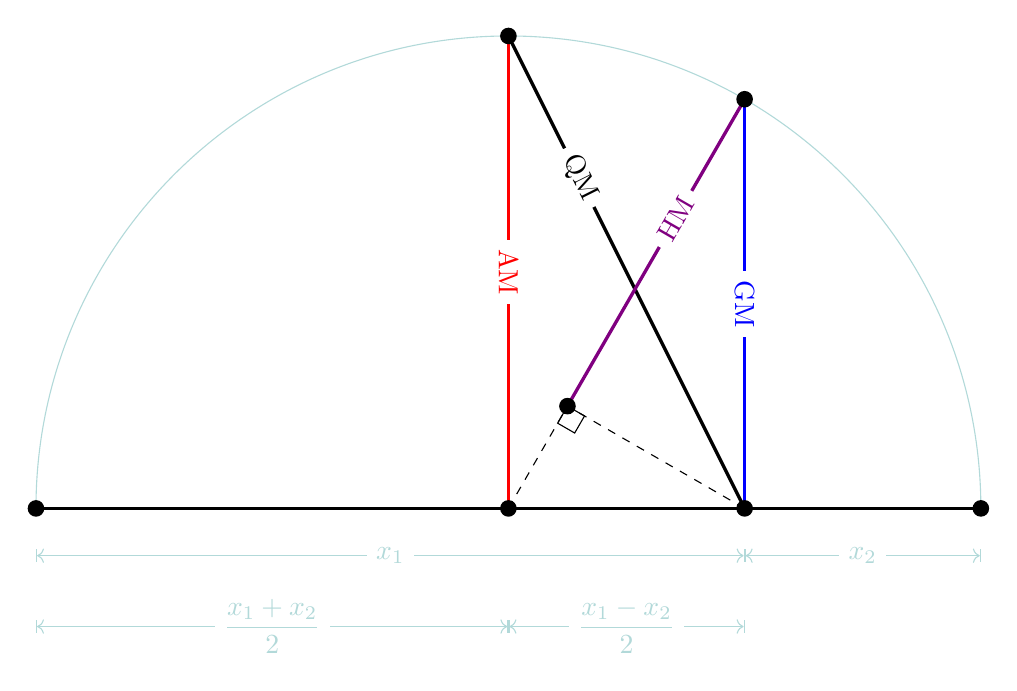
\begin{tikzpicture}[scale=1.0]
    \draw[help lines](-6,0)--(6,0) arc (0:180:6);
    \draw[help lines,|<->|](-6,-0.6)--(3,-0.6) node[midway,fill=white]{$x_1$};
    \draw[help lines,|<->|](3,-0.6)--(6,-0.6) node[midway,fill=white]{$x_2$};
    \draw[help lines,|<->|](-6,-1.5)--(0,-1.5)node[midway,fill=white]{$\dfrac{x_1+x_2}2$};
    \draw[help lines,|<->|](0,-1.5)--(3,-1.5)node[midway,fill=white]{$\dfrac{x_1-x_2}2$};
    \coordinate (G) at (60:6);
    \coordinate (H) at (60:1.5);
    \tkzDefPoint(3,0){C}
    \tkzDefPoint(0,0){O}
    \tkzMarkRightAngle[draw,fill=white](O,H,C)
    \draw[very thick, blue](G)--(C) node[sloped,midway,fill=white]{GM};
    \draw[very thick, red](0,6)--(0,0) node[midway,sloped,fill=white]{AM};
    \draw[very thick](0,6)--(C) node[sloped,pos=0.3,fill=white]{QM};
    \draw[very thick, violet](H)--(G) node[sloped,pos=0.61,fill=white]{HM};
    \draw[very thick](-6,0)--(6,0);
    \fill (-6,0) circle(3pt);
    \fill (C) circle(3pt);
    \fill (6,0) circle(3pt);
    \fill (G) circle(3pt);
    \fill (H) circle(3pt);
    \fill (0,6) circle(3pt);
    \fill (O) circle(3pt);
    \draw[dashed](0,0)--(H);
    \draw[dashed](3,0)--(H);
  \end{tikzpicture}
  \caption{$n=2$时HM,GM,AM,QM的几何示意}
  \label{fig:HM-GM-AM-QM}
\end{figure}

\begin{lemma}\label{lemma:b-1-a}
  若$b\le1\le a$,则$ab\le a+b-1$。
\end{lemma}
\begin{proof}
  由$0\le (a-1)(1-b)=a+b-ab-1$可得。此引理比较重要,被应用到很多不等式的证明过程中。
\end{proof}

\begin{lemma}\label{lemma:product-ai-ge-n}
  $\forall a_i>0$,若满足$\prod_{i=1}^n a_i=1$,则以下不等式成立
  \begin{align}
    \sum_{i=1}^n a_i\ge n
  \end{align}
  当且仅当$a_1=a_2=\cdots=a_n=1$时上述等号成立。
\end{lemma}
\begin{proof}
  对$n$作数学归纳。当$n=1$时显然。当$n\ge2$时,不妨对$a_i$重新排列使得$a_1\equiv\max(a_1,a_2,\cdots,a_n)\ge1$,$a_2\equiv\min(a_1,a_2,\cdots,a_n)\le1$,那么以下$n-1$个数的序列
  \begin{align*}
    a_1a_2, a_3, a_4, \cdots, a_n
  \end{align*}
  满足$n-1$的情况,从而有
  \begin{align*}
    a_1a_2 + a_3+ a_4+ \cdots + a_n &\ge n-1
  \end{align*}
  当且仅当$a_1a_2=a_3=a_4=\cdots=a_n=1$时等号成立,又由引理\ref{lemma:b-1-a},$a_1+a_2 - 1\ge a_1a_2$,其中等号当且仅当$a_1=1$或者$a_2=1$时成立。代入后有
  \begin{align*}
    (a_1 + a_2 - 1) + a_3+ a_4+ \cdots + a_n &\ge n-1\\
    a_1 + a_2 + \cdots + a_n\ge n
  \end{align*}
  其中等号成立,当且仅当以下两个条件同时满足:
  \begin{enumerate}
  \item $a_1a_2=a_3=a_4=\cdots=a_n=1$
  \item $a_1=1$或者$a_2=1$
  \end{enumerate}
  由此条件可知当且仅当所有的$a_i$都等于1时等号成立。
\end{proof}

下面证明AM-GM不等式。
\begin{proof}
  令$g\equiv\sqrt[n]{\prod\limits_{i=1}^n a_i}$,对序列
  \begin{align*}
    \frac{a_1}{g}, \frac{a_2}{g}, \frac{a_3}{g}, \cdots, \frac{a_n}{g}
  \end{align*}
  应用引理\ref{lemma:product-ai-ge-n},有
  \begin{align*}
    \frac{a_1}{g} + \frac{a_2}{g} + \frac{a_3}{g} + \cdots + \frac{a_n}{g}&\ge n\\
    \frac{a_1 + a_2 + a_3 + \cdots + a_n}{n}&\ge g = \sqrt[n]{a_1a_2a_3\cdots a_n} \qedhere
  \end{align*}
\end{proof}

对于三角形,HM还有以下几何意义:
\begin{example}
  对任意三角形,其内切圆的半径是三角形三条高长度的调和平均值的三分之一,即
  \begin{align*}
    r=\frac13 HM(h_a,h_b,h_c)
  \end{align*}
\end{example}
\begin{proof}
  尝试用面积来解,如图~\ref{fig:incircle}所示设三边边长分别是$a,b,c$,
  其对应的高分别为 $h_a, h_b, h_c$,则三角形面积$S=\frac12
  ah_a = \frac12 bh_b = \frac12 ch_c$,同样有$S=\frac12 r(a+b+c)$,从而
  \begin{align*}
    & S = \frac12 r\left( \frac{2S}{h_c} +\frac{2S}{h_a} + \frac{2S}{h_b} \right)
    \quad \implies\quad  r=\frac{1}{\dfrac1{h_a} + \dfrac1{h_b} + \dfrac1{h_c}} \qedhere
  \end{align*}
\end{proof}

\begin{figure}[htbp]
  \centering
  \begin{tikzpicture}[scale=1]
    \tkzDefPoint[label=below left:$A$](0,0){A}
    \tkzDefPoint[label=below right:$B$](6,0){B}
    \tkzDefPoint[label=above:$C$](5,5){C}
    
    \tkzDefCircle[in](A,B,C)\tkzGetPoint{I}\tkzGetLength{rIN}
    \tkzDrawCircle[R](I,\rIN pt);
    \tkzDrawSegments(A,B B,C C,A)
    \tkzDrawSegments[dashed](I,A I,B I,C)
    \tkzDrawCircle[fillstyle=solid,R](I,2pt)

    \coordinate(IA) at ($(B)!(I)!(C)$);
    \coordinate(IB) at ($(C)!(I)!(A)$);
    \coordinate(IC) at ($(A)!(I)!(B)$);

    \tkzDrawSegments[dashed](I,IA I,IB I,IC)
    \tkzMarkRightAngle[color=blue](B,IC,I)
    \tkzMarkRightAngle[color=blue](C,IA,I)
    \tkzMarkRightAngle[color=blue](A,IB,I)
  \end{tikzpicture}
  \caption{三角形内切圆}
  \label{fig:incircle}
\end{figure}

\begin{example}
  若任意非负数$a,b,c$满足$(a+1)(b+1)(c+1)=8$,则$abc\le 1$。
\end{example}
\begin{proof}
  若$a,b,c$均非负,则由AM-GM不等式,有$a+1\ge 2\sqrt{a}$,从而
  \begin{align*}
    8=(a+1)(b+1)(c+1)\ge 2\sqrt{a}\times 2\sqrt{b} \times 2\sqrt{c}
  \end{align*}
  即$abc\le1$。当且仅当$a=b=c=1$时等号成立。
\end{proof}

上述条件不能扩展到任意实数,$a,b,c$一负两正或者三个都是负数,则显然$abc<0$;但对
于$a,b,c$两负一正,比如$a=-2,b=-2,c=7$,则$abc>1$。



\begin{question}\label{q:1/1+a+b}
  三个正数$a,b,c$的乘积是1,求证
  \begin{align*}
    \frac1{1+a+b} + \frac1{1+b+c} + \frac1{1+c+a} \le 1
  \end{align*}
  当且仅当$a=b=c=1$时等号成立。
\end{question}

先尝试猜测每一项的上界。
\begin{align*}
  1+a+b\ge 3\sqrt[3]{ab},\quad 1+b+c \ge 3\sqrt[3]{bc},\quad 1+c+a\ge 3\sqrt[3]{ca}
\end{align*}
从而
\begin{align*}
  \frac1{1+b+c} + \frac1{1+c+a} + \frac1{1+a+b} \le
  \frac13\left( \frac1{\sqrt[3]{ab}} + \frac1{\sqrt[3]{bc}} + \frac1{\sqrt[3]{ca}} \right)
\end{align*}
令$a\to0+, b\to 0+, c=\frac1{ab}$,则上式$\le$符号右边$\to+\infty$,从而没上界,此估计无用。

% 又任意正数$x,y$,有
% \begin{align*}
%   \sqrt{xy}\ge \frac2{\dfrac1x + \dfrac1y}%
%   % \implies  \frac1{xy}\le \frac2{\dfrac1{x^2} + \dfrac1{y^2}}
% \end{align*}

% 令$a_0=\sqrt[6]a, b_0=\sqrt[6]b, c_0=\sqrt[6]c$,代入,有
% \begin{align*}
%   \frac1{\sqrt[3]{ab}} = \frac1{\sqrt{a_0b_0}}\le \frac2{\dfrac1{a_0} + \dfrac1{b_0}}
%   =\frac{2a_0b_0}{a_0+b_0}
% \end{align*}
% 同理处理$\frac1{\sqrt[3]{bc}}$和$\frac1{\sqrt[3]{ca}}$,从而有
% \begin{align*}
%   \frac1{1+b+c} + \frac1{1+c+a} + \frac1{1+a+b} \le
%   \frac23 \left(
%   \frac{a_0b_0}{a_0+b_0} + \frac{b_0c_0}{b_0+c_0} + \frac{c_0a_0}{c_0+a_0} 
%   \right)
% \end{align*}
% 其中$a_0b_0c_0=1$,且上式当且仅当$a_0=b_0=c_0=1$时等号成立。{\color{red}往下似乎不好走了,尝试换个方法。}


\begin{lemma}
对任意$a,b,c\in\mathcal{R}$,有以下恒等式:
\begin{align*}
  (a+b+c)(ab+bc+ca)&=a^2b+a^2c+b^2c+b^2a+c^2a+c^2b + 3abc\\
                   &=(a+b)(b+c)(c+a)+abc
\end{align*}
\end{lemma}
\begin{proof}
  左右分别展开可得证。
\end{proof}

令$x=b+c, y=c+a, z=a+b$,代入有
\begin{align*}
  & \frac1{1+b+c}+\frac1{1+c+a}+\frac1{1+a+b}\le 1\\
  \iff & \underline{(1+x)(1+y)} + (1+y)(1+z) + (1+z)(1+x) \le \underline{(1+x)(1+y)(1+z)}\\
  \iff & \underline{z(1+x)(1+y)} - \underline{(1+y)(1+z)} - (1+z)(1+x) \ge 0\\
  \iff & \underline{zx(1+y)} - (1+y) - 1-x-z-\underline{zx}\ge 0\\
  \iff & zxy - 2 - (x+y+z)\ge 0\\
  \iff & (a+b)(b+c)(c+a) - 2 - 2(a+b+c)\ge 0\\
  \iff & (a+b+c)(ab+bc+ca) - abc -2(a+b+c)\ge 2 \quad(\text{把}abc=1\text{代入})\\
  \iff & (a+b+c)(ab+bc+ca-2)\ge 3
  % \iff & (1+c+a)(1+a+b) + (1+b+c)(1+a+b) + (1+b+c)(1+c+a) \le (1+b+c)(1+c+a)(1+a+b)\\
  % \iff & (b+c)(1+c+a)(1+a+b) - (1+b+c)(1+a+b) - (1+b+c)(1+c+a) \ge 0\\
  % \iff & (b+c)(c+a)(1+a+b) - (1+a+b) - (1+b+c)(1+c+a) \ge 0\\
  % \iff & (b+c)(c+a)(a+b) - (1+a+b) - (1+c+a) - (b+c) \ge 0\\
  % \iff & (b+c)(c+a)(a+b) - 2(1+a+b+c)\ge 0\\
  % \iff & cab+b^2c+a^2b+ab^2 +c^2a+bc^2+a^2c+abc - 2(1+a+b+c)\ge 0\\
  % \iff & b^2c+a^2b+ab^2 +c^2a+bc^2+a^2c - 2(a+b+c)\ge 0\\
  % \iff & (a+b+c)(ab+bc+ca)-3abc -2(a+b+c)\ge 0\\
  % \iff & (a+b+c)(ab+bc+ca-2)\ge 3
\end{align*}
而由AM-GM不等式,有$a+b+c\ge 3\sqrt[3]{abc}=3, ab+bc+ca\ge 3\sqrt[3]{ab\cdot bc\cdot ca}=3$,可得。


\begin{question}
  上题中能否推广到任意正整数$n$,若正数$a_1,a_2,\cdots,a_n$的乘积是$1$,且令$S$表示其和,即
  \begin{align*}
    S\equiv\sum_{i=1}^n a_i
  \end{align*}
  则有
  \begin{align*}
    \sum_{i=1}^n \frac{1}{1 - a_i + S}\le 1
  \end{align*}
  当且仅当$a_1=a_2=\cdots=a_n=1$时等号成立?
\end{question}

当$n=1$时,$a_1=1$,有
\begin{align*}
  \sum_{i=1}^n \frac{1}{1 - a_i + S} = \frac{1}{1} = 1
\end{align*}

当$n=2$时,由$a_1a_2=1$,代入后恒有
\begin{align*}
  \sum_{i=1}^n \frac{1}{1 - a_i + S} &= \frac{1}{1+a_2} + \frac1{1+a_1}\\
                                     &= \frac{1+a_1 + 1 + a_2}{(1+a_1)(1+a_2)}\\
                                     &=1
\end{align*}

当$n=3$时,由题\ref{q:1/1+a+b}已得证。若用引理\ref{lemma:product-ai-ge-n},有$S\ge 3$,从而
\begin{align*}
  \sum_{i=1}^n \frac{1}{1 - a_i + S} &\le \sum_{i=1}^n \frac{1}{1 - a_i + 3}\\
                                     &=   \sum_{i=1}^n \frac{1}{4 - a_i}\\
\end{align*}
{\color{red}上式可不一定,比如$a_i>4$呢?这方法不一定可行。}

用数学归纳法。设$n\le k$时成立,考虑$n=k+1$的情况。考虑数列$\{a_1,a_2,\cdots, a_{k-1}, a_ka_{k+1}\}$,共$k$个数,且其乘积为$1$,从而有
\begin{align*}
  \sum_{i=1}^{k} \frac{1}{1 - a_i' + S_{k+1}'}
\end{align*}
其中
\begin{align*}
  a_i'=
  \begin{cases}
    a_i &i=1,2,\cdots,k-1\\
    a_ka_{k+1} &i=k
  \end{cases} \quad
  S_{k+1}'= a_1+a_2+\cdots +a_{k-1} + a_ka_{k+1}
\end{align*}

%%%%%%%%%%%%%%%%%%%%%%%%%%%%%%%%%%%%%%%%
%%% Basic inequality examples
%%%%%%%%%%%%%%%%%%%%%%%%%%%%%%%%%%%%%%%%
\begin{example}
  证明对$\forall a,b,c\in\mathcal{R}$,有$a^2+b^2+c^2\ge ab+bc+ca$。
\end{example}
\begin{proof}
  由AM--GM不等式,有
\begin{align*}
  a^2+b^2\ge 2ab,\quad b^2+c^2\ge 2bc,\quad c^2+a^2\ge 2ca
\end{align*}
三式相加并除以2可得。该不等式可以推广:$\forall n>1, x_i\in\mathcal{R}(i=1,2,\cdots,n)$,有
\begin{align*}
  \sum_{i=1}^n x_i^2\ge \sum_{i=1}^n x_ix_{i+1}
\end{align*}
其中$x_{n+1}=x_1$。
\end{proof}

\begin{example}
  对任意非负数$a,b$及正整数$n\ge2$,有 $(n-1)a^n + b^n\ge na^{n-1}b$。
\end{example}
对序列$a^n,a^n,\cdots,a^n,b^n$(其中有$n-1$项$a^n$应用AM-GM不等式,有)
\begin{align*}
  \underbrace{a^n + a^n + \cdots + a^n}_{n-1\text{个}} + b^n \ge
  n\times \sqrt[n]{\left(a^n\right)^{n-1} b^n}
  = na^{n-1}b
\end{align*}
当$n=3,4,5$时,有
\begin{align*}
  2a^3 + b^3&\ge 3a^2b\\
  3a^4 + b^4&\ge 4a^3b\\
  4a^5 + b^5&\ge 5a^4b
\end{align*}

\begin{example}
  若正数$a,b,c$的乘积为$1$,求$ab+bc+ca$的极值。
\end{example}
\begin{proof}[提示]
\begin{align*}
  ab+bc+ca\ge 3\times\sqrt[3]{ab\cdot bc\cdot ca}=3\times\sqrt[3]{(abc)^2}=3
\end{align*}
当且仅当$a=b=c=1$时等号成立。另一方面,令$a=b=n,c=1/n^2$,则
\begin{align*}
  ab+bc+ca>ab=n^2\to+\infty (n\to+\infty)
\end{align*}
即$ab+bc+ca$无上界。
\end{proof}


\begin{example}
  若正数$a,b,c$的乘积为$1$,求$a+b+c$的极值。
\end{example}
\begin{align*}
  a+b+c\ge 3\times\sqrt[3]{abc}=3
\end{align*}
当且仅当$a=b=c=1$时等号成立。另一方面,令$a=b=n,c=1/n^2$,则
\begin{align*}
  a+b+c>a=n\to+\infty(n\to+\infty)
\end{align*}
即$a+b+c$无上界。

\begin{example}
  找出所有满足下列等式的实数$a,b,c,d$
  \begin{align*}
    a^2+b^2+c^2+d^2=a(b+c+d)
  \end{align*}
\end{example}

$\forall a,b,c,d\in\mathcal{R}$,有
\begin{align*}
  \left(\frac a2\right)^2\ge 0,\quad \left(\frac a2\right)^2 + b^2\ge ab,
  \quad \left(\frac a2\right)^2 + c^2\ge ac, \quad \left(\frac a2\right)^2 + d^2\ge ad
\end{align*}
四式相加,有
\begin{align*}
  a^2+b^2+c^2+d^2\ge a(b+c+d)
\end{align*}
当且仅当$a=0, \frac a2=b=c=d$时即$a=b=c=d=0$时成立。即原题只有$a=b=c=d=0$这一个解。

\begin{example}
  若正数$a,b,c$的平方和为1,求下式的最小值
  \begin{align*}
    S=\frac{a^2b^2}{c^2} + \frac{b^2c^2}{a^2} + \frac{c^2a^2}{b^2}
  \end{align*}
\end{example}

由
\begin{align*}
  \frac{a^2b^2}{c^2} + \frac{b^2c^2}{a^2}\ge 2b^2,\quad
  \frac{b^2c^2}{a^2} + \frac{c^2a^2}{b^2}\ge 2c^2,\quad
  \frac{c^2a^2}{b^2} + \frac{a^2b^2}{c^2}\ge 2a^2
\end{align*}
三式相加并除以2,有
\begin{align*}
  S\ge a^2+b^2+c^2=1
\end{align*}
当且仅当$\dfrac{a^2b^2}{c^2} = \dfrac{b^2c^2}{a^2} = \dfrac{c^2a^2}{b^2}$即$a=b=c=\frac1{\sqrt3}$时等号成立。


\begin{example}
  $x,y$是小于1的正数,则
  \begin{align*}
    \frac1{1-x^2} + \frac1{1-y^2} \ge \frac2{1-xy}
  \end{align*}
\end{example}
由$x+y\ge2\sqrt{xy}$,有
\begin{align*}
  \frac1{1-x^2} + \frac1{1-y^2} &\ge \frac2{\sqrt{(1-x^2)(1-y^2)}} &&\text{等号成立}\iff x=\pm y\\
  &=\frac2{\sqrt{1+x^2y^2-x^2-y^2}} \\
  &\ge \frac2{\sqrt{1+x^2y^2-2xy}} &&\text{等号成立}\iff x=y\\
  &=\frac2{\sqrt{(1-xy)^2}} \\
  &=\frac2{1-xy}
\end{align*}
当且仅当$x=y$时等号成立。

\begin{example}
  对任意非负数$a,b$,有
  \begin{align*}
    a^3+b^3\ge a^2b+ab^2
  \end{align*}
  推广:对任意非负数$a,b,c$,有
  \begin{align*}
    a^3+b^3+c^3\ge a^2b+b^2c+c^2a
  \end{align*}
  上述结论对任意$n>1$个非负数$a_1,a_2,\cdots,a_n$是否成立,即
  \begin{align*}
    \sum_{i=1}^n a_i^3\ge a_1^2a_2 + a_2^2a_3 + \cdots + a_{n-1}^2a_n + a_n^2a_1
  \end{align*}
\end{example}
由$a^3+b^3-a^2b-ab^2=a^2(a-b)+b^2(b-a)=(a-b)^2(a+b)\ge0$可得,当且仅当$a=b$时等号成立。

由$2a^3+b^3\ge3a^2b$,轮换$a,b,c$,有
\begin{align*}
  2a^3+b^3\ge3a^2b,\quad 2b^3+c^3\ge3b^2c,\quad 2c^3+a^3\ge3c^2a
\end{align*}
三式相加并除以3可得。

\begin{theorem}[Shapiro不等式,Shapiro's Cyclic Inequalities]
  $n$是正整数,序列$\{x_1,x_2,\cdots,x_n\}$是正数序列,则
  \begin{enumerate}
  \item 若$n$是正奇数且$3\le n\le 23$,则
    \begin{align*}
      \sum_{i=1}^{n} \frac{x_i}{x_{i+1} + x_{i+2}} \ge \frac{n}{2}  
    \end{align*}
    其中$x_{n+1} = x_1, x_{n+2} = x_2$。当且仅当$x_1=x_2=\cdots=x_n$时等号成立;

  \item 若$n$且正偶数且$4\le n\le 12$,则
    \begin{align*}
      \sum_{i=1}^{n} \frac{x_i}{x_{i+1} + x_{i+2}} \ge \frac{n}{2}  
    \end{align*}
    当且仅当$x_1=x_3=x_5=\cdots=x_{n-1}$且$x_2=x_4=x_6=\cdots=x_n$时等号成立;

  \item 若$n$是大于12的偶数或者是大于23的奇数,则存在正数序列$\{x_1,x_2,\cdots,x_n\}$,使得
    \begin{align*}
      \sum_{i=1}^{n} \frac{x_i}{x_{i+1} + x_{i+2}} < \frac{n}{2}  
    \end{align*}
  \end{enumerate}
\end{theorem}
\begin{proof}[说明]
  这里仅说明一下其证明历史。B.~A.~Troesch在1989年证明了(1),P.~J.~Bushell \& J.~B.~McLeod在2002年证明了(2),而(3)则是早在1979年就被 J.~L.~Searcy \& B.~A.~Troesch所证明。
\end{proof}

\begin{example}[Nesbitt不等式]
  对任意正数$a,b,c$,有
  \begin{align*}
    \frac{a}{b+c}+\frac{b}{c+a}+\frac{c}{a+b}\ge\frac32
  \end{align*}
\end{example}
\begin{proof}[提示]
  这是Shapiro不等式在$n=3$时的情形。有多种巧妙的证明方法。下面是其中三种。
  \begin{enumerate}
  \item 利用凸函数的Jensen不等式。记$S=a+b+c$,则
    \begin{align*}
      f(x)=\frac{x}{S-x}
    \end{align*}
    在$x\in[0,S)$上是凸的,应用Jensen不等式,则有
    \begin{align*}
      \frac{f(a) + f(b) + f(c)}{3}\ge f\left(\frac{a+b+c}{3}\right)=f\left(\frac{S}{3}\right)=\frac12
    \end{align*}
  \item 用换元法,消除难处理的分母。令$x=a+b,y=b+c,z=c+a$,则$x,y,z$是正数,且有
    \begin{align*}
      a=\frac{x-y+z}2,\quad b=\frac{x+y-z}2,\quad c=\frac{-x+y+z}2
    \end{align*}
    代入,有
    \begin{align*}
      \frac{a}{b+c}+\frac{b}{c+a}+\frac{c}{a+b}
      &= \frac{x-y+z}{2y} + \frac{x+y-z}{2z} + \frac{-x+y+z}{2x}\\
      &= \frac12\left(\frac{x+z}{y} + \frac{x+y}{z} + \frac{y+z}{x}\right)-\frac32\\
      &= \frac12\left( \underbrace{\left(\frac xy + \frac yx\right)}_{\text{应用AM--GM不等式}}
        +\left(\frac zy + \frac yz\right)
        +\left(\frac xz + \frac zx\right)
        \right)-\frac32\\
      &\ge \frac12\times ( 2 + 2 + 2) - \frac32=\frac32
      % &=\frac32
    \end{align*}
    当且仅当$\dfrac xy=\dfrac yx$, $\dfrac zy=\dfrac yz$, $\dfrac xz=\dfrac zx$即$x=y=z$时等号成立,亦即$a=b=c$时等号成立。

  \item 直接利用AM--HM不等式。由
    \begin{align*}
      & \frac{(a+b)+(b+c)+(c+a)}{3}\ge \frac{3}{\dfrac1{a+b}+\dfrac1{b+c}+\dfrac1{c+a}}\\
      \iff & \big[(a+b)+(b+c)+(c+a)\big]\left(\dfrac1{a+b}+\dfrac1{b+c}+\dfrac1{c+a}\right)\ge 9\\
      \iff & 2(a+b+c)\left(\dfrac1{a+b}+\dfrac1{b+c}+\dfrac1{c+a}\right)\ge 9\\
      \iff & 2\left(1+\dfrac{c}{a+b}+1+\dfrac{a}{b+c}+1+\dfrac{b}{c+a}\right)\ge 9
    \end{align*}
    展开可得。其等号成立的充要条件是$a+b=b+c=c+a$,即$a=b=c$。$\qedhere$
  \end{enumerate}
\end{proof}

\begin{question}
  证明Shapiro不等式在$n=4$时的情况,即对任意正数$a,b,c,d$,有
  \begin{align*}
    \frac{a}{b+c}+\frac{b}{c+d}+\frac{c}{d+a}+\frac{d}{a+b}\ge 2
  \end{align*}
\end{question}
% \begin{proof}[提示]
%   应用\ref{lemma:titu}的T2引理,有
%   \begin{align*}
%          &\frac{a}{b+c}+\frac{b}{c+d}+\frac{c}{d+a}+\frac{d}{a+b}\\
%     =\   &\frac{a^2}{a(b+c)}+\frac{b^2}{b(c+d)}+\frac{c^2}{c(d+a)}+\frac{d^2}{d(a+b)}\\
%     \ge\ &\dfrac{(a+b+c+d)^2}{a(b+c) + b(c+d) + c(d+a) + d(a+b)}
%   \end{align*}

%   \begin{align*}
%        & \frac{a}{b+c}+\frac{b}{c+d}+\frac{c}{d+a}+\frac{d}{a+b}\\
%     =\ & \left(\frac{a}{b+c}+\frac{c}{d+a}\right) + \left(\frac{b}{c+d}+\frac{d}{a+b}\right)\\
%     \ge\ & \dfrac{(a+c)^2}{a(b+c)+c(d+a)} + \dfrac{(b+d)^2}{b(c+d)+d(a+b)}\\
%     =\ & \dfrac{a^2+2ac+c^2}{ab+ac+cd+da}
%   \end{align*}
% \end{proof}

% 同样应用换元法简化分母,令$w=a+b$,$x=b+c$,$y=c+d$,$z=d+a$。先反求用$w$,$x$,$y$和$z$表示$a$:
% \begin{enumerate}
% \item 先看$w$,比$a$多了个$b$;
% \item $x$有$b$,$w-x=a-c$,又多减了个$c$;
% \item $y$里有$c$,$w-x+y=a+d$,则又多加了个$d$;
% \item $z$里有$d$,$w-x+y-z=2a$,多加了个$a$。
% \end{enumerate}
% 从而有$a=(w-x+y-z)/2$。类似地,有
% \begin{align*}
%   a&=\frac{w-x+y-z}2 & b&=\frac{x-y+z-w}2\\
%   c&=\frac{y-z+w-x}2 & d&=\frac{z-w+x-y}2
% \end{align*}
% 代入,有
% \begin{align*}
%      &\frac{a}{b+c}+\frac{b}{c+d}+\frac{c}{d+a}+\frac{d}{a+b}\\
%   =\ &\frac{w-x+y-z}{2x} + \frac{x-y+z-w}{2y} + \frac{y-z+w-x}{2z} + \frac{z-w+x-y}{2w}\\
%   =\ &\frac12\left( \frac{w+y-z}{x} + \frac{x+z-w}{y} + \frac{y+w-x}{z} + \frac{z+x-y}{w} - 4\right)
% \end{align*}
% 有负号,不能直接应用AM--GM不等式。代入继续化简,要证明的不等式等价于
% \begin{align*}
%        & \frac12\left( \frac{w+y-z}{x} + \frac{x+z-w}{y} + \frac{y+w-x}{z} + \frac{z+x-y}{w} - 4\right) \ge 2\\
%   \iff & \frac{w+y-z}{x} + \frac{x+z-w}{y} + \frac{y+w-x}{z} + \frac{z+x-y}{w} \ge 8\\
%   \iff & wyz(w+y-z) + xzw(x+z-w) + ywx(y+w-x) + zxy(z+x-y) \ge 8wxyz\\
%   \iff & w^2(yz-xz+xy) + x^2(wz-wy+yz) + y^2(
% \end{align*}


% {\color{red}似乎没用?}


\begin{question}
  证明:对任意正数$a,b,c$,有
  \begin{align*}
    \frac{a^3}{a^2+ab+b^2}+\frac{b^3}{b^2+bc+c^2}+\frac{c^3}{c^2+ca+a^2}
    \ge
    \frac{a+b+c}{3}
  \end{align*}
\end{question}

\begin{question}
  对任意正数$a_1,a_2,\cdots,a_n,b_1,b_2,\cdots,b_n$,有
  \begin{align*}
    \sum_{i=1}^n\frac{a_ib_i}{a_i+b_i}\le
    \frac{\sum\limits_{i=1}^n a_i \cdot \sum\limits_{i=1}^n b_i}
         {\sum\limits_{i=1}^n a_i + \sum\limits_{i=1}^n b_i}
  \end{align*}
\end{question}
对$n$用数学归纳法。

\begin{question}
  若$a_1,a_2,\cdots,a_n,b_1,b_2,\cdots,b_n$是正数,则
  \begin{align*}
    \sum_{i=1}^n \sqrt{a_ib_i}
    \le
    \sqrt{\sum_{i=1}^n a_i \cdot \sum_{i=1}^n b_i}
  \end{align*}
\end{question}
对$n$用数学归纳法。

\begin{question}
  对正数$a,b,c$,证明
  \begin{align*}
    \frac{5a^3-ab^2}{a+b} & \ge 3a^2-b^2\\
    \frac{5a^3-ab^2}{a+b} + \frac{5b^3-bc^2}{b+c} + \frac{5c^3-ca^2}{c+a} & \ge 2(a^2+b^2+c^2)
  \end{align*}
\end{question}
只需证明第一条即可,而第一条又等价于$2a^3+b^3\ge 3a^2b$。

\begin{question}
  对大于$2$的整数$n$,及非负数$x_1,x_2,\cdots,x_n$,若$x_1=0, x_n=1$,则存在整数$j\in[1,2,\cdots,n-1]$,使得
  \begin{align*}
    \left| x_{j-1} - 2x_j + x_{j+1} \right| \ge \frac{4}{n^2}
  \end{align*}
\end{question}
令$x_0=0,x_{n+1}=1$,且对$k=0,1,2,\cdots,n$,令$y_k=x_{k+1}-x_k$,则$y_0=y_n=0$,且$y_0+y_1+y_2+\cdots+y_n=1$。用反证法。假设对所有的$j=1,2,\cdots,n$,不等式不成立,从而有
\begin{align*}
  y_j - y_{j-1} \le \left| y_j-y_{j-1} \right| = \left| x_{j-1} - 2x_j + x_{j+1} \right| < \frac{4}{n^2}
\end{align*}
对$j=1,2,\cdots,k$加起来,则有
\begin{align*}
  y_k&=y_k-y_0=(y_1-y_0) + (y_2-y_1) + \cdots + (y_k-y_{k-1})\\
  &<\underbrace{\frac{4}{n^2}+\frac{4}{n^2}+\cdots+\frac{4}{n^2}}_{k\text{个}}\\
  &=\frac{4k}{n^2}
\end{align*}
同样$y_{j-1}-y_j<\frac{4}{n^2}$,加起来,有
\begin{align*}
  y_k&=y_{k}-y_n=(y_k-y_{k+1})+(y_{k+1}-y_{k+2})+\cdots+(y_{n-1}-y_{n})\\
  &<\underbrace{ \frac{4}{n^2}+\frac{4}{n^2}+\cdots+\frac{4}{n^2}}_{n-k\text{个}}\\
  &=\frac{4(n-k)}{n^2}
\end{align*}

若$n$是奇数,则
\begin{align*}
  1&=y_0+y_1+y_2+\cdots+y_n\\
  &=\left(y_1+y_1+\cdots+y_{\frac{n-1}2}\right)
  + \left(y_{\frac{n+1}2}+y_{\frac{n+1}2+1}+\cdots+y_n\right)\\
  & <\frac4{n^2}\left(
  \left(1+2+\cdots+\frac{n-1}2\right) +
  \left( \left(n-\frac{n+1}2\right) + \left(n-\frac{n+1}2-1\right) + \cdots + 1\right)
  \right)\\
  &=2\cdot\frac4{n^2}\left(1+2+\cdots+\frac{n-1}2\right)\\
  &=\frac8{n^2}\left( \left(1+\frac{n-1}2\right)\cdot\frac{n-1}2\cdot\frac12 \right)\\
  &=\frac{n^2-1}{n^2}<1
\end{align*}
矛盾。

若$n$是偶数,则
\begin{align*}
  1&=y_0+y_1+y_2+\cdots+y_n\\
  &=\left(y_1+y_1+\cdots+y_{\frac{n}2-1}\right)
  + \left(y_{\frac{n}2+1}+y_{\frac{n}2+2}+\cdots+y_n\right)
\end{align*}
剩余略。



\chapter{勾股数}
\label{chap:pythagorean_triples}

\begin{definition}[勾股数]
  若正整数$a,b,c$满足$a^2+b^2=c^2$,则称$a,b,c$为勾股数。
\end{definition}

勾股数也称为毕达哥拉斯三元组(Pythagorean Triples)。常见的勾股数有
\begin{align*}
  (3,4,5),\quad (5,12,13)
\end{align*}

\begin{property}
  $a,b,c$是勾股数,则
  \begin{enumerate}
  \item 若$a,b,c$三者的最大公约数是1,则$a,b,c$两两互质。
  \end{enumerate}
\end{property}

\begin{proof}
  略。
\end{proof}

\begin{definition}[Primitive Pythagorean Triples]
  勾股数$a,b,c$若两两互质,则称$a,b,c$为原始毕达哥拉斯三元组。
\end{definition}

\begin{lemma}
  $\forall n\in\mathcal{Z}^+, 4n+2$不是完全平方数。
\end{lemma}

\begin{proof}
  $4n+2=2(2n+1)$,而$2n+1$是奇数,即$4n+2$的因式分解中2的幂是奇数1,从而$4n+2$不可能是完全平方数。
\end{proof}

\begin{lemma}
  若$(a,b,c)$是原始毕达哥拉斯三元组,则$a,b$必是一奇一偶。
\end{lemma}

\begin{proof}
  首先排除$a,b$都是偶数的情况,否则$c$也是偶数,这样$(a,b,c)$不互质。再次排除$a,b$都是奇数的情况。假如$a,b$都是奇数,则$a^2\equiv b^2\equiv 1(\mod 4)$,从而$c^2\equiv 1 + 1\equiv 2(\mod 4)$不是一个完全平方数,矛盾。
\end{proof}

\begin{theorem}[Euclid's Formula]
  对任意整数$m>n>0$,则以下三元组是Pythagorean三元组
  \begin{align*}
    a=m^2-n^2,\quad b=2mn,\quad c=m^2+n^2
  \end{align*}
\end{theorem}

\begin{proof}
  略。按定义立得。
\end{proof}

\begin{theorem}\label{th:pythagorean-triples}
  若$(a,b,c)$是原始勾股数,且$a$是奇数,$b$是偶数,则存在两个互质且奇偶相反的整数$m>n>0$,使得
  \begin{align*}
    a=m^2-n^2,\quad b=2mn,\quad c=m^2+n^2
  \end{align*}
\end{theorem}

由此定理可知,原始勾股数都可以由Euclid公式生成。

\begin{proof}
  由于$b$是偶数,$a,c$都是奇数,从而$c\pm a$都是偶数,且有
  \begin{align*}
    \left(\frac b2\right)^2 = \frac{c+a}2\times\frac{c-a}2
  \end{align*}
  
  先证明$\dfrac{c\pm a}2$是互质的,否则存在整数$d>1$整除两数的和(等于$c$)与差(等于$a$),从而$c$和$a$有大于1的公约数$d$,与$(a,b,c)$两两互质矛盾。从而存在$m,n\in\mathcal{Z}^+$,使得
  \begin{align*}
    \frac{c+a}2=m^2,\quad \frac{c-a}2=n^2
  \end{align*}
  由上式得到$(a,b,c)$由$m,n$的表达式,后续过程以及请自行补充完整。

  关于$m,n$的奇偶性不同,首先由$m,n$互质排除两者都是偶数;若都是奇数,则由上面的表达式,$(a,b,c)$三者均为偶数,与$(a,b,c)$两两互质矛盾。从而$m,n$奇偶性不同。
\end{proof}


\begin{example}[1965 Putnam Exam.]
  面积的数值是其周长数值的两倍,且边长是整数的直角三角形总共只有3个。
\end{example}

\begin{proof}
  由定理\ref{th:pythagorean-triples},可设满足条件的三角形边长由下式给出
  \begin{align*}
    a = (m^2-n^2)d,\quad b=2mnd,\quad c=(m^2+n^2)d
  \end{align*}
  其中$d$是三边长的最大公约数,$m,n$满足定理\ref{th:pythagorean-triples}中的条件。再由面积的数值是周长数值的两倍,从而有
  \begin{align*}
    \frac12 \times (m^2-n^2)d\times 2mnd & = 2\left( (m^2-n^2)d + 2mnd + (m^2+n^2)d \right)\\
    \implies (m-n)nd & = 4
  \end{align*}
  由于$m-n$是奇数,从而$m-n=1$,又$n$是4的因数可取$1,2,4$,从而$m,n,d$的有以下三种组合
  \begin{align*}
    (2,1,4),\quad (3,2,2),\quad (5,4,1)
  \end{align*}
  此时对应的三角边长分别是
  \begin{align*}
    (12,16,20),\quad (10,24,26),\quad (9,40,41)
  \end{align*}
  即只有上述三种三角形。
\end{proof}

\begin{example}[1975 IMO]
  证明单位圆上任意两点间距离是有理数的点的集合可以有无限个元素。
\end{example}

\hints 令$A=(1,0),B=(-1,0),O$是原点。考虑
\begin{align*}
  \mathcal{P}\equiv\{p:AP=\frac{2(m^2-n^2)}{m^2+n^2}, BP=frac{4mn}{m^2+n^2}
\end{align*}
其中$m,n$满足定理\ref{th:pythagorean-triples},求$\mathcal{P}$中任意两点距离。

\begin{example}[Wiadom. Mat.(1955/56), pp.194-5, Polish]
  求$3^x+4^y=5^z$的所有正整数解。
\end{example}

\begin{proof}
  首先证明$z$是偶数。考虑模3的余数,有
  \begin{align*}
    1 \equiv 0 + 1^y \equiv 3^x + 4^y \equiv 5^z \equiv (-1)^z \tag*{$\pmod 3$}
  \end{align*}
  从而$z$必须是偶数,设$z=2w$,其中$w\in\mathcal{Z}^+$。从而有
  \begin{align*}
    3^x = 5^{2w} - 4^y = \left(5^w\right)^2 - \left(2^y\right)^2 = \left(5^w + 2^y\right)\left(5^w - 2^y\right)
  \end{align*}
  由于$(5^w + 2^y) + (5^w - 2^y) = 2\times 5^w$不能被3整除,从而$5^w + 2^y$和$5^w - 2^y$中有一个不能被3整除,再由上式,可知
  \begin{align*}
    5^w-2^y =1,\quad 5^w+2^y =3^x
  \end{align*}
  上式对3取模,有
  \begin{align*}
    (-1)^w - (-1)^y &= 1 \tag*{$\pmod 3$}\\
    (-1)^w + (-1)^y &= 0 \tag*{$\pmod 3$}\\
  \end{align*}
  从而$w$是奇数,$y$是偶数(请自行考虑)。若$y>2$,则
  \begin{align*}
     5^w\equiv 5^w+2^y \equiv 3^x \equiv 1\text{或者}3 \tag*{$\pmod 8$}
  \end{align*}
  又$w$是奇数,从而存在非负整数$u$,使得$w=2u + 1$,从而有
  \begin{align*}
    5^w \equiv 5^{2u + 1} \equiv 5\times 25^u \equiv 5\times (24 + 1)^u \equiv 5 \tag*{$\pmod 8$}
  \end{align*}
  两个结果矛盾,从而$y=2$。而由$5^w-2^y=1$,有$w=1$,从而$z=2w=2$,$x=2$。
\end{proof}

\section{平面几何五大模型}
\label{sec:five-models-in-geometry}

\subsection{等积模型}
\label{sec:same-volumne-model}

\begin{theorem}
  两个三角形若等底等高,则其面积相等。
\end{theorem}

\begin{theorem}
  两个三角形若底相同,则其面积比等于高的比;两个三角形若高相同,则其面积比等于对应底的比。
\end{theorem}

这两个结论由三角形面积公式(底乘高除以2)显然可得。


\subsection{鸟头模型}
\label{sec:common-angle-theorem}

\begin{definition}[共角三角形]
  两三角形若有一个角相等或互补,则称这两个三角形为共同三角形。
\end{definition}

\begin{theorem}[共角定理,鸟头定理]
  共角三角形的面积比等于相等或互补的角的两夹边的乘积比。
\end{theorem}
\begin{proof}
  由三角形的另一面积公式$S=\dfrac12ab\sin C$,结论显然成立。
\end{proof}

\begin{example}
  如图,其中线段长度如标示,求阴影部分与非阴影部分的面积比。

  \centering
  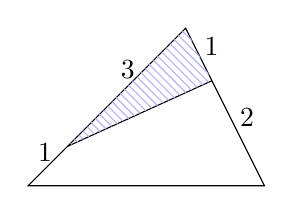
\begin{tikzpicture}[scale=1.0]
    \begin{scope}[shift={(0,0)}]
      \coordinate (A) at (2,2);
      \coordinate (B) at (0,0);
      \coordinate (C) at (3,0);
      \coordinate (D) at ($.75*(B) + .25*(A)$);
      \coordinate (E) at ($2/3*(A) + 1/3*(C)$);
      \draw(E)--(D)
              --(B)node[pos=.15,left]{$1$}
              --(C)
              --(E)node[pos=.65,right]{$2$}
              --(A)node[pos=.65,right]{$1$}
              --(D)node[pos=.35,left]{$3$};
      \fill[pattern=north west lines,pattern color=blue!30](A)--(D)--(E)--cycle;
    \end{scope}
  \end{tikzpicture}
\end{example}
\begin{proof}[解]
  由共角定理,阴影部分与大三角形面积比为
  \begin{align*}
    \frac{3\times 1}{(3+1)\times(1+2)}=\frac{3}{3\times4}=\frac14
  \end{align*}
  从而在大三角形中,阴影部分面积占$\dfrac14$,非阴影部分点$\dfrac34$,阴影与非阴影面积之比为$1:3$。
\end{proof}

\begin{question}
  以下图形的阴影与非阴影面积之间的比例关系同样可应用鸟头定理,请自行思考。

  \centering
  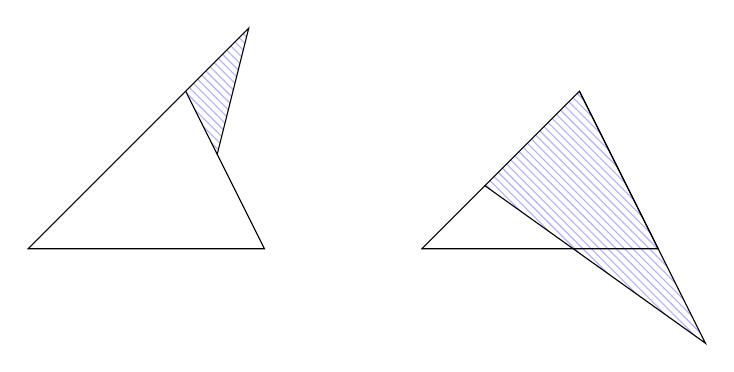
\begin{tikzpicture}[scale=1.0]
    \begin{scope}[shift={(0,0)}]
      \coordinate(A) at (2,2);
      \coordinate(B) at (0,0);
      \coordinate(C) at (3,0);
      \coordinate(D) at ($.4*(C)+.6*(A)$);
      \coordinate(E) at ($1.4*(A)$);
      \draw[pattern=north west lines,pattern color=blue!30](A)--(D)--(E)--cycle;
      \draw(D)--(C)--(B)--(A);
    \end{scope}

    \begin{scope}[shift={(5,0)}]
      \coordinate(A) at (2,2);
      \coordinate(B) at (0,0);
      \coordinate(C) at (3,0);
      \coordinate(D) at ($1.6*(C)-.6*(A)$);
      \coordinate(E) at ($.4*(A)$);
      \draw[pattern=north west lines,pattern color=blue!30](A)--(D)--(E)--cycle;
      \draw(A)--(C)--(B)--(E);
    \end{scope}

    \begin{scope}[shift={(8,0)}]
      
    \end{scope}
  \end{tikzpicture}
\end{question}


\subsection{蝴蝶模型}
\label{sec:butterfly-theorem}

\begin{theorem}[蝴蝶定理]
  如图,任意凸四边形的对角线将四边形分成$4$个小三角形,则其面积$S_1,S_2,S_3,S_4$满足以下关系
  \begin{align*}
    S_1S_3=S_2S_4
  \end{align*}

  \centering
  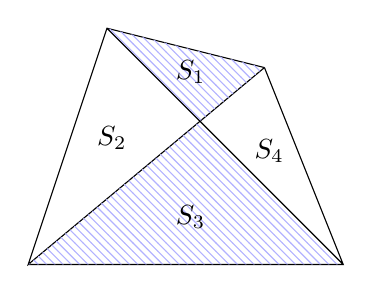
\begin{tikzpicture}[scale=1.0]
    \coordinate(A)at(0,0);
    \coordinate(B)at(4,0);
    \coordinate(C)at(3,2.5);
    \coordinate(D)at(1,3);
    \draw(A)--(B)--(C)--(D)--(A)--(C) (B)--(D);
    \tkzInterLL(A,C)(B,D)\tkzGetPoint{O}
    \fill[pattern=north west lines,pattern color=blue!30](A)--(O)--(B)--cycle;
    \fill[pattern=north west lines,pattern color=blue!30](C)--(O)--(D)--cycle;
    \node at ($1/3*(D)+1/3*(A)+1/3*(O)$) {$S_2$};
    \node at ($1/3*(A)+1/3*(B)+1/3*(O)$) {$S_3$};
    \node at ($1/3*(B)+1/3*(C)+1/3*(O)$) {$S_4$};
    \node at ($1/3*(C)+1/3*(D)+1/3*(O)$) {$S_1$};
  \end{tikzpicture}
\end{theorem}
\begin{proof}
  找三角形的同底或等高关系,可得$\dfrac{S_1}{S_2}=\dfrac{S_4}{S_3}$,变换一下即得证。
\end{proof}

\begin{example}[梯形中的蝴蝶定理]
  如图,梯形中的上下底边长分别为$a$和$b$,则对角线分成的$4$个小三角形的面积有如下关系:
  \begin{align*}
    S_1:S_2:S_3:S_4=a^2:ab:b^2:ab
  \end{align*}

  \centering
  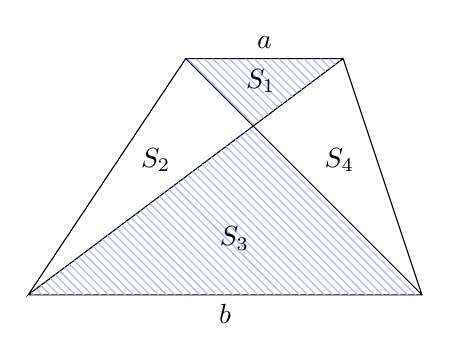
\begin{tikzpicture}[scale=1.0]
    \coordinate(A)at(0,0);
    \coordinate(B)at(5,0);
    \coordinate(C)at(4,3);
    \coordinate(D)at(2,3);
    \draw(A)--(B) node[midway,below]{$b$}--(C)--(D) node[midway,above]{$a$}--(A)--(C) (B)--(D);
    \tkzInterLL(A,C)(B,D)\tkzGetPoint{O}
    \fill[pattern=north west lines,pattern color=blue!30](A)--(O)--(B)--cycle;
    \fill[pattern=north west lines,pattern color=blue!30](C)--(O)--(D)--cycle;
    \node at ($1/3*(D)+1/3*(A)+1/3*(O)$) {$S_2$};
    \node at ($1/3*(A)+1/3*(B)+1/3*(O)$) {$S_3$};
    \node at ($1/3*(B)+1/3*(C)+1/3*(O)$) {$S_4$};
    \node at ($1/3*(C)+1/3*(D)+1/3*(O)$) {$S_1$};
  \end{tikzpicture}
\end{example}
\begin{proof}
  首先由三角形相似性,有$S_1:S_3=a^2:b^2$。其次$S_2+S_3$与$S_4+S_3$同底等高从而面积相等,也就是$S_2=S_4$。再由蝴蝶定理,并令$S_1=a^2$,从而有$S_3=b^2$,并且
  \begin{align*}
    S_1\cdot S_3=S_2\cdot S_4\implies a^2 \cdot b^2 = S_2^2\implies S_2=ab&\qedhere
  \end{align*}
\end{proof}


\subsection{燕尾模型(swallowtaile-theore??????)}
\label{sec:swallowtail-theore}


\begin{theorem}[燕尾定理]
  如图,$D,E,F$分别是三角形$ABC$三边上一点,且$AD$、$BE$与$CF$有共同的交点$O$,则
  \begin{align*}
    S_{\triangle ABO}:S_{\triangle ACO} = S_{\triangle OBD}:S_{\triangle OCD} = BD:CD
  \end{align*}
  其余三角形有类似结论。
  
  \centering
  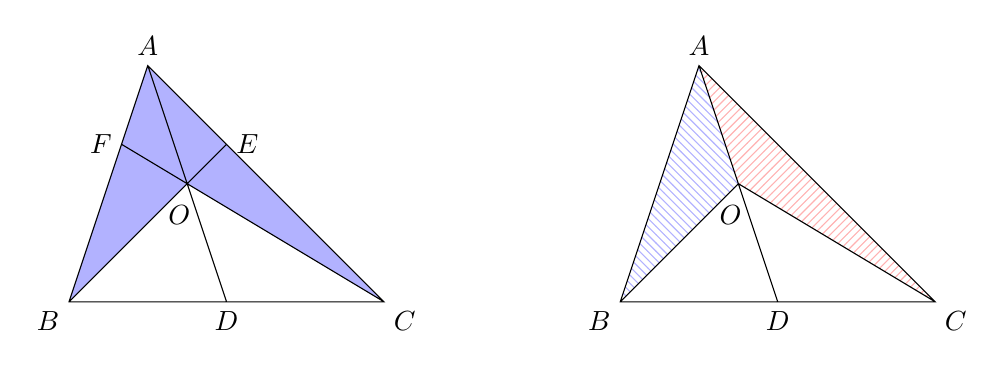
\begin{tikzpicture}[scale=1.0]
    \begin{scope}[shift={(0,0)}]
      \coordinate(A)at(1,3);
      \coordinate(B)at(0,0);
      \coordinate(C)at(4,0);
      \coordinate(O)at(1.5,1.5);
      \tkzInterLL(A,O)(B,C)\tkzGetPoint{D}
      \tkzInterLL(B,O)(C,A)\tkzGetPoint{E}
      \tkzInterLL(C,O)(A,B)\tkzGetPoint{F}
      \fill[color=blue!30](A)--(B)--(O)--(C)--(A);
      \draw(A)--(B)--(C)--cycle (A)--(D) (B)--(E) (C)--(F);
      \tkzLabelPoints[above](A)
      \tkzLabelPoints[below left](B)
      \tkzLabelPoints[below right](C)
      \tkzLabelPoints[below](D)
      \tkzLabelPoints[right](E)
      \tkzLabelPoints[left](F)
      \node at($(O) + (-.1,-.4)$) {$O$};
    \end{scope}

    \begin{scope}[shift={(7,0)}]
      \coordinate(A)at(1,3);
      \coordinate(B)at(0,0);
      \coordinate(C)at(4,0);
      \coordinate(O)at(1.5,1.5);
      \tkzInterLL(A,O)(B,C)\tkzGetPoint{D}
      \tkzInterLL(B,O)(C,A)\tkzGetPoint{E}
      \tkzInterLL(C,O)(A,B)\tkzGetPoint{F}
      \fill[pattern=north west lines,pattern color=blue!30](A)--(B)--(O);
      \fill[pattern=north east lines,pattern color=red!30](A)--(C)--(O);
      \draw(A)--(B)--(C)--cycle (A)--(D) (B)--(O) (C)--(O);
      \tkzLabelPoints[above](A)
      \tkzLabelPoints[below left](B)
      \tkzLabelPoints[below right](C)
      \tkzLabelPoints[below](D)
      % \tkzLabelPoints[right](E)
      % \tkzLabelPoints[left](F)
      \node at($(O) + (-.1,-.4)$) {$O$};
    \end{scope}
  \end{tikzpicture}
\end{theorem}
\begin{proof}[说明]
  如第二图的最小模型,若只考虑一个燕尾,可在$AD$上随意取点$O$即有上述结论,即无需知道$E,F$两点。
\end{proof}

\begin{example}
  在燕尾定理的图中,燕尾$ABOC$的面积与$\triangle ABC$的面积比等于$AO:AD$。
\end{example}
\begin{proof}[提示]
  将燕尾沿$AD$切成两边分别考虑,有
  \begin{align*}
    \frac{S_{\triangle AOB}}{S_{\triangle ADB}} = \frac{AO}{AD},\quad
    \frac{S_{\triangle AOC}}{S_{\triangle ADC}} = \frac{AO}{AD}
  \end{align*}
  两式分子分母分别相加可得\footnote{这里用到了这样一个结论:若$a_1/b_1=a_2/b_2$,则$(a_1+a_2)/(b_1+b_2)=a_1/b_1$。当然,这里$b_1$和$b_2$需要满足一定条件,请自行思考。}。
\end{proof}

\begin{example}
  在燕尾定理的图中,证明
  \begin{align*}
    \frac{BD}{DC}\times\frac{CE}{EA}\times\frac{AF}{FB}=1
  \end{align*}
\end{example}
\begin{proof}
  由燕尾定理,有
  \begin{align*}
    S_{\triangle ABO}:S_{\triangle ACO} &= BD:DC\\
    S_{\triangle ACO}:S_{\triangle CBO} &= AF:FB\\
    S_{\triangle CBO}:S_{\triangle ABO} &= CE:EA
  \end{align*}
  三式相乘可得。
\end{proof}


\begin{example}
  已知$\triangle ABC$中,$AE:EF:FB=1:3:2$,$D$是$BC$的中点,且图中阴影部分$S_{EFHG}=51$,求$\triangle ABC$的面积$S_{\triangle ABC}$。
  \begin{center}
    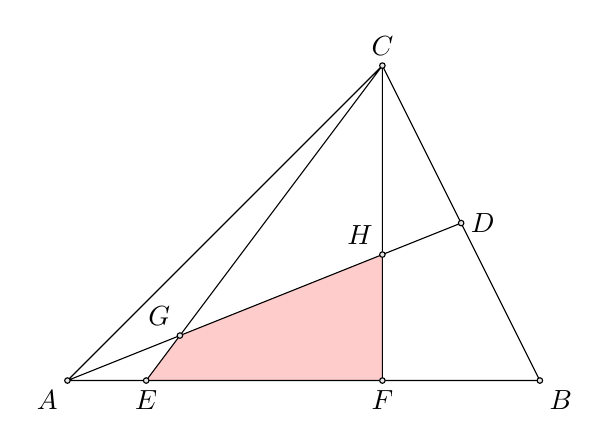
\begin{tikzpicture}[scale=1.0]
      \coordinate(A)at(0,0);\coordinate(E)at(1,0);\coordinate(F)at(4,0);\coordinate(B)at(6,0);
      \coordinate(C)at(4,4);\coordinate(D)at(5,2);
      \tkzInterLL(A,D)(C,E)\tkzGetPoint{G}
      \tkzInterLL(A,D)(C,F)\tkzGetPoint{H}
      \fill[color=red!20](E)--(F)--(H)--(G)--cycle;
      \draw(A)--(B)--(C)--(A)--(D) (E)--(C)--(F);
      \tkzDrawPoints(A,B,C,D,E,F,G,H);
      \foreach \L/\P in{A/below left, B/below right, C/above, D/right, E/below, F/below, G/above left, H/above left}{
        \tkzLabelPoints[\P](\L)
      }
    \end{tikzpicture}
  \end{center}
\end{example}

\begin{proof}[提示]
  解法一,可用燕尾定理,关键是得到$AG:GH:HD$。考虑燕尾$CAHB$的两边,如下图:
  \begin{center}
    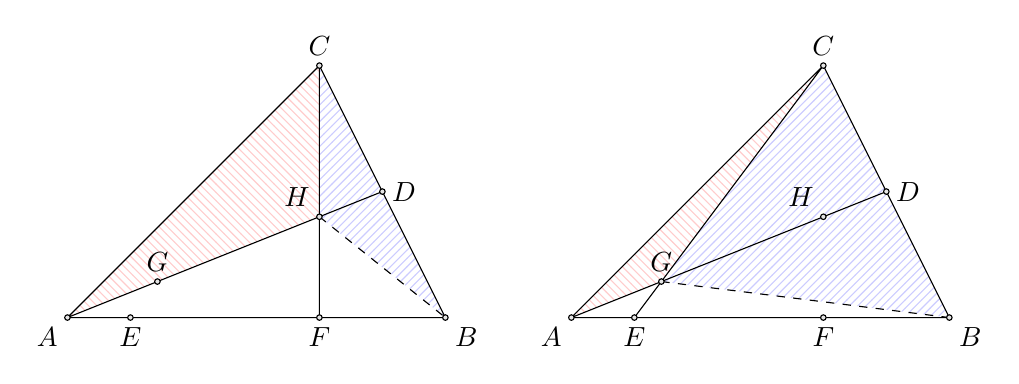
\begin{tikzpicture}[scale=.8]
      \begin{scope}
        \coordinate(A)at(0,0);\coordinate(E)at(1,0);\coordinate(F)at(4,0);\coordinate(B)at(6,0);
        \coordinate(C)at(4,4);\coordinate(D)at(5,2);
        \tkzInterLL(A,D)(C,E)\tkzGetPoint{G}
        \tkzInterLL(A,D)(C,F)\tkzGetPoint{H}
        % \fill[color=red!20](E)--(F)--(H)--(G)--cycle;
        \fill[pattern=north west lines, pattern color=red!20](C)--(A)--(H);
        \fill[pattern=north east lines, pattern color=blue!20](C)--(B)--(H);
        \draw(A)--(B)--(C)--(A)--(D) (C)--(F);
        \draw[dashed](H)--(B);
        \tkzDrawPoints(A,B,C,D,E,F,G,H);
        \foreach \L/\P in{A/below left, B/below right, C/above, D/right, E/below, F/below, G/above, H/above left}{
          \tkzLabelPoints[\P](\L)
        }
      \end{scope}
      \begin{scope}[shift={(8,0)}]
        \coordinate(A)at(0,0);\coordinate(E)at(1,0);\coordinate(F)at(4,0);\coordinate(B)at(6,0);
        \coordinate(C)at(4,4);\coordinate(D)at(5,2);
        \tkzInterLL(A,D)(C,E)\tkzGetPoint{G}
        \tkzInterLL(A,D)(C,F)\tkzGetPoint{H}
        % \fill[color=red!20](E)--(F)--(H)--(G)--cycle;
        \fill[pattern=north west lines, pattern color=red!20](C)--(A)--(G);
        \fill[pattern=north east lines, pattern color=blue!20](C)--(B)--(G);
        \draw(A)--(B)--(C)--(A)--(D) (C)--(E);
        \draw[dashed](G)--(B);
        \tkzDrawPoints(A,B,C,D,E,F,G,H);
        \foreach \L/\P in{A/below left, B/below right, C/above, D/right, E/below, F/below, G/above, H/above left}{
          \tkzLabelPoints[\P](\L)
        }
      \end{scope}
    \end{tikzpicture}
  \end{center}
  则有
  \begin{align*}
    S_{\triangle CHA}:S_{\triangle CHB} = AF:FB = (1+3):2=2
  \end{align*}
  由$D$是$BC$中点,可知$S_{\triangle BHD}=S_{\triangle CHD}$,代入有
  \begin{align*}
    S_{\triangle CAH}:(2\times S_{\triangle CHD}) = 2\implies
    S_{\triangle CAH}:S_{\triangle CHD} = 4
  \end{align*}
  从而有$AH:HD=4$。同样的,由燕尾$CAGB$,有
  \begin{align*}
    S_{\triangle CGA}:S_{\triangle CGD} ={}& 2\times( S_{\triangle CGA}:S_{\triangle CGB} )\\
    ={}& 2\times( AE:EB ) = 2\times( 1 : (3+2))=2:5
  \end{align*}
  由此可得$AG:GH:HD$。实际上,$AG$占整个$AD$的$\frac27$,$HD$占整个$AD$的$\frac15$,所以$GH$占整个$AD$的$1-\frac27-\frac15$,由此可得三者的比例为$10:18:7$。从而由共角定理有
  \begin{align*}
    &S_{\triangle AEG} : S_{\triangle AFH} : S_{\triangle ABD}\\
    =&(1\times 10) : ((1+3)\times(10+18)) : ((1+3+2)\times(10+18+7))\\
    =&10 : 112 : 210
  \end{align*}
  由此可得
  \begin{align*}
    S_{\triangle AEG} : S_{EFHG} : S_{FBDH} ={}& 10 : (112-10) : (210-112)\\
    ={}& 10:102:98=5:51:49
  \end{align*}
  现已知$S_{EFHG}=51$,从而有
  \begin{align*}
    S_{\triangle AEG}={}&5\\
    S_{FBDH}         ={}&49\\
    S_{\triangle ABD}={}&5+51+49=105\\
    S_{\triangle ABC}={}&2\times 105=210
  \end{align*}

  类似地也通过求得$CG:GE$及$CH:HF$,来得到原图中各小部分的面积比。

  方法二,可作各种平行线,求得各线段的比例关系。

  方法三可用梅涅劳斯定理。
\end{proof}

\begin{theorem}
  如图,$\triangle ABC$中,$D$和$E$分别是$AB$和$AC$上一点,$CD$和$BE$交于点$F$。若$AD:DB=x:y$,$AE:EC=u:v$,则
  \begin{align*}
    \frac{CF}{FD} = \dfrac{\frac{x}{y}}{1+\frac{u}{v}},\qquad\qquad
    \frac{BF}{FE} = \dfrac{\frac{u}{v}}{1+\frac{x}{y}}
  \end{align*}
  \begin{center}
    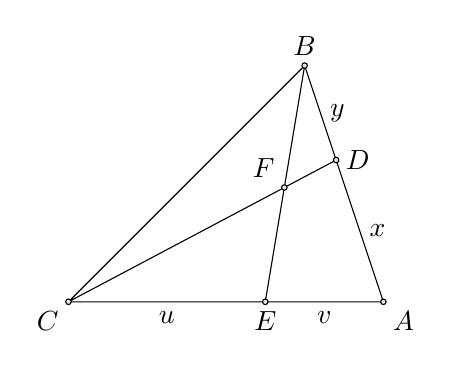
\begin{tikzpicture}[scale=1.0]
      \coordinate(A)at(4,0);\coordinate(B)at(3,3);\coordinate(C)at(0,0);
      \coordinate(D)at($0.4*(A)+0.6*(B)$);\coordinate(E)at(2.5,0);
      \tkzInterLL(C,D)(B,E)\tkzGetPoint{F}
      \draw(A)--(D) node[midway,right]{$x$}
              --(B) node[midway,right]{$y$}
              --(C)
              --(E) node[midway,below]{$u$}
              --(A) node[midway,below]{$v$}
           (C)--(D) (B)--(E);
      \tkzDrawPoints(A,B,C,D,E,F)
      \foreach \L/\P in{A/below right, B/above, C/below left, D/right, E/below, F/above left}{
        \tkzLabelPoints[\P](\L)
      }
    \end{tikzpicture}
  \end{center}
\end{theorem}

\begin{proof}
  连接$AF$,考虑燕尾$BCFA$,有$S_{\triangle BAF}:S_{\triangle BCF} = x:y$,把$S_{\triangle AFD}:S_{\triangle BFD}=u:v$代入,有
  \begin{align*}
    \dfrac{(1 + \frac{u}{v})S_{\triangle BFD}}{S_{\triangle BCF}} = \frac{x}{y}
  \end{align*}
  从而
  \begin{align*}
    \frac{CF}{FD}=\dfrac{S_{\triangle BFD}}{S_{\triangle BCF}} = \dfrac{\frac{x}{y}}{1+\frac{u}{v}}&\qedhere
  \end{align*}
\end{proof}

\begin{example}
  记$P$为$\forall\triangle ABC$内任意一点,且$AP$、$BP$及$CP$分别与$\triangle ABC$的三边相交于$D$、$E$及$F$。求
  \begin{align*}
    \frac{AP}{AD} + \frac{BP}{BE} + \frac{CP}{CF} = ?
  \end{align*}
  \centering
  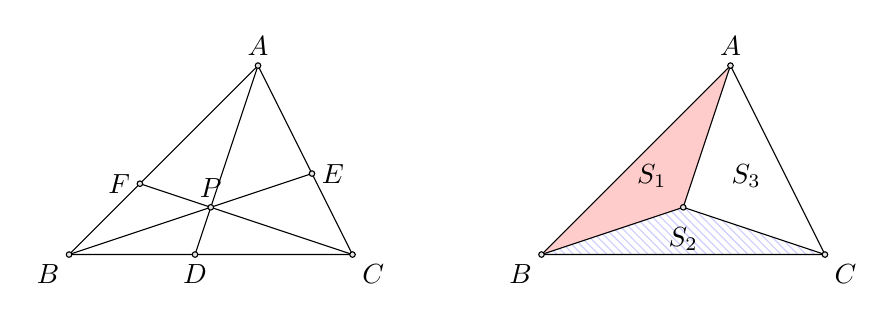
\begin{tikzpicture}[scale=1.2]
    \begin{scope}
      \coordinate[label=above:$A$](A)at(2,2);
      \coordinate[label=below left:$B$](B)at(0,0);
      \coordinate[label=below right:$C$](C)at(3,0);
      \coordinate[label=above:$P$](P)at(1.5,.5);
      \tkzInterLL(A,P)(B,C)\tkzGetPoint{D}
      \tkzInterLL(B,P)(C,A)\tkzGetPoint{E}
      \tkzInterLL(C,P)(A,B)\tkzGetPoint{F}
      \draw(A)--(B)--(C)--cycle;
      \draw(A)--(D) (B)--(E) (C)--(F);
      \tkzDrawPoints(A,B,C,D,E,F,P)
      \tkzLabelPoints[below](D)
      \tkzLabelPoints[right](E)
      \tkzLabelPoints[left](F)
    \end{scope}
    \begin{scope}[shift={(5,0)}]
      \coordinate[label=above:$A$](A)at(2,2);
      \coordinate[label=below left:$B$](B)at(0,0);
      \coordinate[label=below right:$C$](C)at(3,0);
      \coordinate(P)at(1.5,.5);
      \tkzInterLL(A,P)(B,C)\tkzGetPoint{D}
      \tkzInterLL(B,P)(C,A)\tkzGetPoint{E}
      \tkzInterLL(C,P)(A,B)\tkzGetPoint{F}
      \fill[color=red!20](A)--(P)--(B)--cycle;
      \fill[pattern=north west lines,pattern color=blue!20](B)--(P)--(C)--cycle;
      \draw(A)--(B)--(C)--cycle;
      \draw(A)--(P) (B)--(P) (C)--(P);
      \tkzDrawPoints(A,B,C,P)
      % \tkzLabelPoints[below](D)
      % \tkzLabelPoints[right](E)
      % \tkzLabelPoints[left](F)
      \node at($1/3*(A)+1/3*(B)+1/3*(P)$){$S_1$};
      \node at($1/3*(B)+1/3*(C)+1/3*(P)$){$S_2$};
      \node at($1/3*(C)+1/3*(A)+1/3*(P)$){$S_3$};
    \end{scope}
  \end{tikzpicture}
\end{example}
\begin{proof}[提示]
  有时长度的比可以转化为面积体积的比。记$S_1\equiv S_{\triangle APB}$,$S_2\equiv S_{\triangle BPC}$,$S_3\equiv S_{\triangle CPA}$,则利用燕尾定理可得
  \begin{align*}
    \frac{AP}{AD}={}\frac{S_1 + S_3}{S_{\triangle ABC}},\quad
    \frac{BP}{BE}={}\frac{S_2 + S_1}{S_{\triangle ABC}},\quad
    \frac{CP}{CF}={}\frac{S_3 + S_2}{S_{\triangle ABC}}
  \end{align*}
  三式相加,可得
  \begin{align*}
    \frac{AP}{AD} + \frac{BP}{BE} + \frac{CP}{CF} = 2&\qedhere
  \end{align*}
\end{proof}

\subsection{相似模型}
\label{sec:similar-model}

?????

\chapter{几何}
\label{chap:geometry}

\begin{example}
  有6个棱长是$3\times4\times5$的相同长方体。现在要把它们的一些面染成红色,要求其中一个染一面,一个染两面,一个染三面,一个染四面,一个染五面,一个染六面。染完后将6个长方体都切成$1\times1\times1$的正方体,问如何染色才能使切出来的正方体中只有一面是红色的个数最多?
\end{example}
\begin{proof}[提示]
  6个正方体分别考虑,使其染完后切成的正方体中含单面红色的最多。
  \begin{enumerate}
  \item 染6面红色的长方体,只有一个染色方案,其中切完后,只有一面是红色的小正方体共有$(2+3+6)\times2=22$个(阴影部分)。

    \begin{center}
      % \tdplotsetmaincoords{70}{120}
      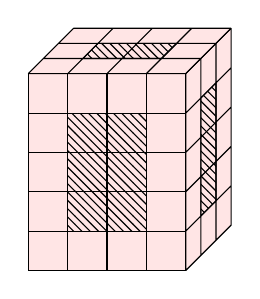
\begin{tikzpicture}[scale=.5,
        % tdplot_main_coords,
        fill red/.style={fill=red, fill opacity=.1},
        slash lines/.style={pattern=north west lines, pattern color=black}]
        \fill[canvas is yz plane at x=4,fill red   ](0,0)rectangle(5,3);
        \draw[canvas is yz plane at x=4,slash lines](1,1)rectangle(4,2);
        \draw[canvas is yz plane at x=4            ](0,0)grid     (5,3);

        \fill[canvas is xz plane at y=5,fill red   ](0,0)rectangle(4,3);
        \draw[canvas is xz plane at y=5,slash lines](1,1)rectangle(3,2);
        \draw[canvas is xz plane at y=5            ](0,0)grid     (4,3);

        \fill[canvas is xy plane at z=3,fill red   ](0,0)rectangle(4,5);
        \draw[canvas is xy plane at z=3,slash lines](1,1)rectangle(3,4);
        \draw[canvas is xy plane at z=3            ](0,0)grid     (4,5);
      \end{tikzpicture}
    \end{center}
    
  \item 只染一个面时,如下图有三种染法。其中第三种染法使得切成小正方体后只有一面是红色的小正方体的数量最多,为$4\times5=20$个。

    \begin{center}
      % \tdplotsetmaincoords{70}{120}
      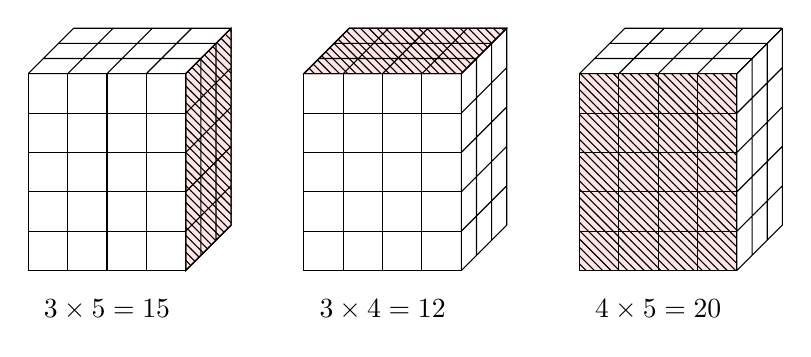
\begin{tikzpicture}[scale=.5,
        % tdplot_main_coords,
        fill red/.style={fill=red, fill opacity=.1},
        slash lines/.style={pattern=north west lines, pattern color=black}]
        \begin{scope}[shift={(0,0)}]
          \fill[canvas is yz plane at x=4,fill red   ](0,0)rectangle(5,3);
          \draw[canvas is yz plane at x=4,slash lines](0,0)rectangle(5,3);
          \draw[canvas is yz plane at x=4            ](0,0)grid     (5,3);

          % \fill[canvas is xz plane at y=5,fill red   ](0,0)rectangle(4,3);
          % \draw[canvas is xz plane at y=5,slash lines](1,1)rectangle(3,2);
          \draw[canvas is xz plane at y=5            ](0,0)grid     (4,3);

          % \fill[canvas is xy plane at z=3,fill red   ](0,0)rectangle(4,5);
          % \draw[canvas is xy plane at z=3,slash lines](1,1)rectangle(3,4);
          \draw[canvas is xy plane at z=3            ](0,0)grid     (4,5) node at(2,-1){$3\times5=15$};
        \end{scope}

        \begin{scope}[shift={(7,0)}]
          % \fill[canvas is yz plane at x=4,fill red   ](0,0)rectangle(5,3);
          % \draw[canvas is yz plane at x=4,slash lines](1,1)rectangle(4,2);
          \draw[canvas is yz plane at x=4            ](0,0)grid     (5,3);

          \fill[canvas is xz plane at y=5,fill red   ](0,0)rectangle(4,3);
          \draw[canvas is xz plane at y=5,slash lines](0,0)rectangle(4,3);
          \draw[canvas is xz plane at y=5            ](0,0)grid     (4,3);

          % \fill[canvas is xy plane at z=3,fill red   ](0,0)rectangle(4,5);
          % \draw[canvas is xy plane at z=3,slash lines](1,1)rectangle(3,4);
          \draw[canvas is xy plane at z=3            ](0,0)grid     (4,5) node at(2,-1){$3\times4=12$};
        \end{scope}

        \begin{scope}[shift={(14,0)}]
          % \fill[canvas is yz plane at x=4,fill red   ](0,0)rectangle(5,3);
          % \draw[canvas is yz plane at x=4,slash lines](1,1)rectangle(4,2);
          \draw[canvas is yz plane at x=4            ](0,0)grid     (5,3);

          % \fill[canvas is xz plane at y=5,fill red   ](0,0)rectangle(4,3);
          % \draw[canvas is xz plane at y=5,slash lines](1,1)rectangle(3,2);
          \draw[canvas is xz plane at y=5            ](0,0)grid     (4,3);

          \fill[canvas is xy plane at z=3,fill red   ](0,0)rectangle(4,5);
          \draw[canvas is xy plane at z=3,slash lines](0,0)rectangle(4,5);
          \draw[canvas is xy plane at z=3            ](0,0)grid     (4,5) node at(2,-1){$4\times5=20$};
        \end{scope}
      \end{tikzpicture}
    \end{center}


  \item 只染两个面时,有如下图三种相邻的染法。其中第三种染法使得切成小正方体后只有一面是红色的小正方体的数量最多,为$5\times\left((4-1)+(3-1)\right)=25$个。

    \begin{center}
      % \tdplotsetmaincoords{70}{120}
      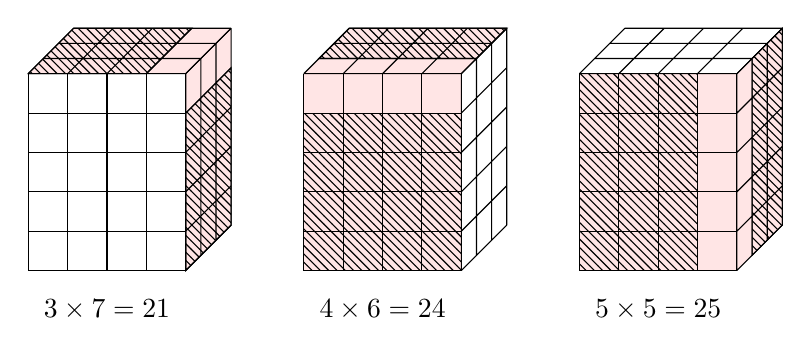
\begin{tikzpicture}[scale=.5,
        % tdplot_main_coords,
        fill red/.style={fill=red, fill opacity=.1},
        slash lines/.style={pattern=north west lines, pattern color=black}]
        \begin{scope}[shift={(0,0)}]
          \fill[canvas is yz plane at x=4,fill red   ](0,0)rectangle(5,3);
          \draw[canvas is yz plane at x=4,slash lines](0,0)rectangle(4,3);
          \draw[canvas is yz plane at x=4            ](0,0)grid     (5,3);

          \fill[canvas is xz plane at y=5,fill red   ](0,0)rectangle(4,3);
          \draw[canvas is xz plane at y=5,slash lines](0,0)rectangle(3,3);
          \draw[canvas is xz plane at y=5            ](0,0)grid     (4,3);

          % \fill[canvas is xy plane at z=3,fill red   ](0,0)rectangle(4,5);
          % \draw[canvas is xy plane at z=3,slash lines](1,1)rectangle(3,4);
          \draw[canvas is xy plane at z=3            ](0,0)grid     (4,5) node at(2,-1){$3\times7=21$};
        \end{scope}

        \begin{scope}[shift={(7,0)}]
          % \fill[canvas is yz plane at x=4,fill red   ](0,0)rectangle(5,3);
          % \draw[canvas is yz plane at x=4,slash lines](1,1)rectangle(4,2);
          \draw[canvas is yz plane at x=4            ](0,0)grid     (5,3);

          \fill[canvas is xz plane at y=5,fill red   ](0,0)rectangle(4,3);
          \draw[canvas is xz plane at y=5,slash lines](0,0)rectangle(4,2);
          \draw[canvas is xz plane at y=5            ](0,0)grid     (4,3);

          \fill[canvas is xy plane at z=3,fill red   ](0,0)rectangle(4,5);
          \draw[canvas is xy plane at z=3,slash lines](0,0)rectangle(4,4);
          \draw[canvas is xy plane at z=3            ](0,0)grid     (4,5) node at(2,-1){$4\times6=24$};;
        \end{scope}

        \begin{scope}[shift={(14,0)}]
          \fill[canvas is yz plane at x=4,fill red   ](0,0)rectangle(5,3);
          \draw[canvas is yz plane at x=4,slash lines](0,0)rectangle(5,2);
          \draw[canvas is yz plane at x=4            ](0,0)grid     (5,3);

          % \fill[canvas is xz plane at y=5,fill red   ](0,0)rectangle(4,3);
          % \draw[canvas is xz plane at y=5,slash lines](1,1)rectangle(3,2);
          \draw[canvas is xz plane at y=5            ](0,0)grid     (4,3);

          \fill[canvas is xy plane at z=3,fill red   ](0,0)rectangle(4,5);
          \draw[canvas is xy plane at z=3,slash lines](0,0)rectangle(3,5);
          \draw[canvas is xy plane at z=3            ](0,0)grid     (4,5) node at(2,-1){$5\times5=25$};;
        \end{scope}
      \end{tikzpicture}
    \end{center}

    还有三种不相邻的染法。由只染一面的结论可知,染两面$5\times4$的两个不相邻面时,切成的小方块只有一面是红色的数量最多,为$5\times4\times2=40$个。

    \begin{center}
      % \tdplotsetmaincoords{70}{120}
      \begin{tikzpicture}[scale=.5,
        % tdplot_main_coords,
        fill red/.style={fill=red, fill opacity=.1},
        slash lines/.style={pattern=north west lines, pattern color=black}]
        \begin{scope}[shift={(0,0)}]
          \fill[canvas is yz plane at x=4,fill red   ](0,0)rectangle(5,3);
          \draw[canvas is yz plane at x=4,slash lines](0,0)rectangle(5,3);
          \draw[canvas is yz plane at x=4            ](0,0)grid     (5,3);
          \draw[canvas is xy plane at z=3,->](-3,2.5)--(-.5,2.5) node[midway,above]{左边};

          % \fill[canvas is xz plane at y=5,fill red   ](0,0)rectangle(4,3);
          % \draw[canvas is xz plane at y=5,slash lines](1,1)rectangle(3,2);
          \draw[canvas is xz plane at y=5            ](0,0)grid     (4,3);

          % \fill[canvas is xy plane at z=3,fill red   ](0,0)rectangle(4,5);
          % \draw[canvas is xy plane at z=3,slash lines](1,1)rectangle(3,4);
          \draw[canvas is xy plane at z=3            ](0,0)grid     (4,5);
        \end{scope}

        \begin{scope}[shift={(7,0)}]
          % \fill[canvas is yz plane at x=4,fill red   ](0,0)rectangle(5,3);
          % \draw[canvas is yz plane at x=4,slash lines](1,1)rectangle(4,2);
          \draw[canvas is yz plane at x=4            ](0,0)grid     (5,3);

          \fill[canvas is xz plane at y=5,fill red   ](0,0)rectangle(4,3);
          \draw[canvas is xz plane at y=5,slash lines](0,0)rectangle(4,3);
          \draw[canvas is xz plane at y=5            ](0,0)grid     (4,3);
          \draw[canvas is xy plane at z=3,->](2,-3)--(2,-.5) node[midway,right]{底面};

          % \fill[canvas is xy plane at z=3,fill red   ](0,0)rectangle(4,5);
          % \draw[canvas is xy plane at z=3,slash lines](1,1)rectangle(3,4);
          \draw[canvas is xy plane at z=3            ](0,0)grid     (4,5);
        \end{scope}

        \begin{scope}[shift={(14,0)}]
          % \fill[canvas is yz plane at x=4,fill red   ](0,0)rectangle(5,3);
          % \draw[canvas is yz plane at x=4,slash lines](1,1)rectangle(4,2);
          \draw[canvas is yz plane at x=4            ](0,0)grid     (5,3);

          % \fill[canvas is xz plane at y=5,fill red   ](0,0)rectangle(4,3);
          % \draw[canvas is xz plane at y=5,slash lines](1,1)rectangle(3,2);
          \draw[canvas is xz plane at y=5            ](0,0)grid     (4,3);

          \fill[canvas is xy plane at z=3,fill red   ](0,0)rectangle(4,5);
          \draw[canvas is xy plane at z=3,slash lines](0,0)rectangle(4,5);
          \draw[canvas is xy plane at z=3            ](0,0)grid     (4,5);
          \draw[canvas is yz plane at x=4,->](2.5,-3)--(2.5,-.5)node[pos=0,right]{背面};
        \end{scope}
      \end{tikzpicture}
    \end{center}
    
  \item 染五面红色只有三种染法(相当于取哪一面不染,与染一面的类似)。

    \begin{center}
      % \tdplotsetmaincoords{70}{120}
      \begin{tikzpicture}[scale=.5,
        % tdplot_main_coords,
        fill red/.style={fill=red, fill opacity=.1},
        slash lines/.style={pattern=north west lines, pattern color=black}]
        \begin{scope}[shift={(0,0)}]
          \fill[canvas is yz plane at x=4,fill red   ](0,0)rectangle(5,3);
          \draw[canvas is yz plane at x=4,slash lines](1,1)rectangle(4,3);
          \draw[canvas is yz plane at x=4            ](0,0)grid     (5,3);

          \fill[canvas is xz plane at y=5,fill red   ](0,0)rectangle(4,3);
          \draw[canvas is xz plane at y=5,slash lines](1,1)rectangle(3,3);
          \draw[canvas is xz plane at y=5            ](0,0)grid     (4,3);

          % \fill[canvas is xy plane at z=3,fill red   ](0,0)rectangle(4,5);
          % \draw[canvas is xy plane at z=3,slash lines](1,1)rectangle(3,4);
          \draw[canvas is xy plane at z=3            ](0,0)grid     (4,5) node at(2,-1){只有前面不染};
        \end{scope}

        \begin{scope}[shift={(7,0)}]
          % \fill[canvas is yz plane at x=4,fill red   ](0,0)rectangle(5,3);
          % \draw[canvas is yz plane at x=4,slash lines](1,1)rectangle(4,2);
          \draw[canvas is yz plane at x=4            ](0,0)grid     (5,3);

          \fill[canvas is xz plane at y=5,fill red   ](0,0)rectangle(4,3);
          \draw[canvas is xz plane at y=5,slash lines](1,1)rectangle(4,2);
          \draw[canvas is xz plane at y=5            ](0,0)grid     (4,3);

          \fill[canvas is xy plane at z=3,fill red   ](0,0)rectangle(4,5);
          \draw[canvas is xy plane at z=3,slash lines](1,1)rectangle(4,4);
          \draw[canvas is xy plane at z=3            ](0,0)grid     (4,5) node at(2,-1){只有右面不染};;
        \end{scope}

        \begin{scope}[shift={(14,0)}]
          \fill[canvas is yz plane at x=4,fill red   ](0,0)rectangle(5,3);
          \draw[canvas is yz plane at x=4,slash lines](1,1)rectangle(5,2);
          \draw[canvas is yz plane at x=4            ](0,0)grid     (5,3);

          % \fill[canvas is xz plane at y=5,fill red   ](0,0)rectangle(4,3);
          % \draw[canvas is xz plane at y=5,slash lines](1,1)rectangle(3,2);
          \draw[canvas is xz plane at y=5            ](0,0)grid     (4,3);

          \fill[canvas is xy plane at z=3,fill red   ](0,0)rectangle(4,5);
          \draw[canvas is xy plane at z=3,slash lines](1,1)rectangle(3,5);
          \draw[canvas is xy plane at z=3            ](0,0)grid     (4,5) node at(2,-1){只有上面不染};;
        \end{scope}
      \end{tikzpicture}
    \end{center}

    第一种,$4\times2(\text{上面加下面})+6\times2(\text{左面加右面})+6(\text{背面})=26$。

    第二种,$3\times2(\text{上面加下面})+9\times2(\text{前面加后面})+3(\text{左面})=27$。

    第三种,$8\times2(\text{前面加后面})+4\times2(\text{左面加右面})+2(\text{底面})=26$。

  \item 染四面红色只有六种染法(相当于取哪两面不染,与染两面的类似)。
  \item 染三面红色时最麻烦,染色方案最多。请自行考虑。
  \end{enumerate}

  六个长方体都讨论完,结论自然就出来了。
\end{proof}

\section{尺规作图}
\label{sec:draw-with-ruler}

\begin{example}
  只用圆规找到给圆的半径。
\end{example}

\begin{example}[上海,1956]
  给定圆周,只用圆规将圆周四等分。
\end{example}

\section{几何不等式}
\label{sec:geometric-inequality}

\subsection{基本不等式}
\label{sec:basic-geometric-inequality}

\begin{theorem}
  平面上两点间直线段长度最短。
\end{theorem}

\begin{example}
  平面上凸四边形$ABCD$,$M,N$分别是$AD$和$BC$的中点,则
  \begin{align*}
    MN\le\frac{AB+CD}{2}
  \end{align*}
  当且仅当$AB\parallel CD$时等号成立。

  \centering
  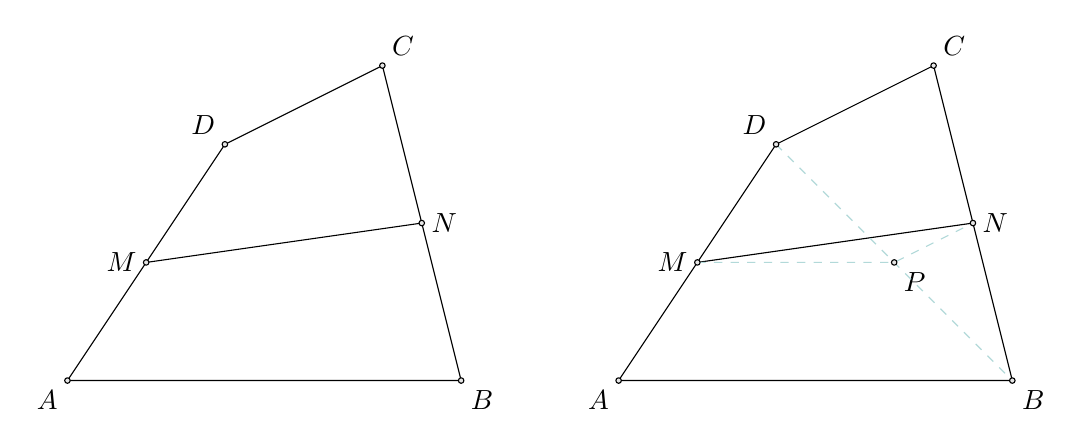
\begin{tikzpicture}[scale=1.0,line join=round]
    \begin{scope}[shift={(0,0)}]
      \coordinate[label=below left:$A$]  (A) at (0,0);
      \coordinate[label=below right:$B$] (B) at (5,0);
      \coordinate[label=above right:$C$] (C) at (4,4);
      \coordinate[label=above left:$D$]  (D) at (2,3);
      \coordinate[label=left:$M$]        (M) at ($.5*(A)+.5*(D)$);
      \coordinate[label=right:$N$]       (N) at ($.5*(B)+.5*(C)$);
      % \coordinate[label=below:$P$] (P) at ($.5*(D)+.5*(B)$);
      \draw(A)--(B)--(C)--(D)--cycle;
      \draw(M)--(N);%--(P)--cycle;
      %\draw(D)--(B);
      \tkzDrawPoints(A,B,C,D,M,N);
    \end{scope}
    \begin{scope}[shift={(7,0)}]
      \coordinate[label=below left:$A$]  (A) at (0,0);
      \coordinate[label=below right:$B$] (B) at (5,0);
      \coordinate[label=above right:$C$] (C) at (4,4);
      \coordinate[label=above left:$D$]  (D) at (2,3);
      \coordinate[label=left:$M$]        (M) at ($.5*(A)+.5*(D)$);
      \coordinate[label=right:$N$]       (N) at ($.5*(B)+.5*(C)$);
      \coordinate[label=below right:$P$] (P) at ($.5*(D)+.5*(B)$);
      \draw(A)--(B)--(C)--(D)--cycle;
      \draw(M)--(N);
      \draw[help lines, dashed](M)--(P)--(N);
      \draw[help lines, dashed](D)--(B);
      \tkzDrawPoints(A,B,C,D,M,N,P);
    \end{scope}
  \end{tikzpicture}
\end{example}
\begin{proof}
  如图取$BD$的点$P$并作辅助线,则
  \begin{align*}
    MN\le MP+NP=\frac{AB+CD}{2}
  \end{align*}
  当且仅当点$P$在$MN$上时等号成立,而$P$在$MN$上时等价于$AB\parallel CD$。
\end{proof}

\begin{theorem}[Pythagorean不等式]
  记三角形的三边分别为$a\le b\le c$,则
  \begin{enumerate}
  \item 三角形是直角三角形$\iff a^2+b^2=c^2$;
  \item 三角形是锐角三角形$\iff a^2+b^2>c^2$;
  \item 三角形是钝角三角形$\iff a^2+b^2<c^2$。
  \end{enumerate}
\end{theorem}
\begin{proof}
  由余弦定理$c^2=a^2+b^2-2ab\cos\mathrm{C}$可得。
\end{proof}


\begin{theorem}[等周不等式,Isoperimetric Inequality]
  若一个平面图形的面积与周长分别为$A$和$P$,则$4\pi A\le P^2$。也就是说在平面上用长度为$P$的线段能围成的最大面积是半径为$\dfrac{P}{2\pi}$的圆,其面积为$\dfrac{P^2}{4\pi}$。
\end{theorem}
\begin{proof}[提示]
  该定理的证明并不平凡,
\end{proof}

\begin{theorem}[三角不等式,Trigonometric Inequality]
  记三角形的三个角分别为$A,B,C$,则
  \begin{align*}
    \sin A +\sin B + \sin C&\le\frac{3\sqrt3}{2}\\
    \cos A +\cos B + \cos C&\le\phantom{3}\,\frac{3}{2}
  \end{align*}
\end{theorem}
\begin{proof}
  由$\sin(x)$及$\cos(x)$在$[0,\pi]$上是凹函数,利用Jensen不等式可得。
\end{proof}

\begin{theorem}[相交弦定理,Intersecting Chords Theorem]
  圆内的两条相交弦,被交点分成的两条线段长的积相等。
\end{theorem}
\begin{proof}
  利用相似三角形可得。
\end{proof}

\begin{theorem}[海伦公式,海伦-秦九韶公式,Heron's Formula]
  记三角形的三边边长分别为$a,b,c$,其半周长$s=\dfrac{a+b+c}2$,则三角形的面积为
  \begin{align}
    S=\sqrt{s(s-a)(s-b)(s-c)}
  \end{align}
\end{theorem}
\begin{proof}
  用余弦公式可证。或者用勾股定理证明$c$边对应的高
  \begin{align*}
    h=\frac{4s(s-a)(s-b)(s-c)}{c^2} &\qedhere
  \end{align*}
\end{proof}

\begin{theorem}
  如图~\ref{fig:r-of-incircle}所示,三角形内切圆将各边分别分割成$x,y,z$的长度,则可得到内切圆的半径公式
  \begin{align}
    r=\sqrt{\frac{xyz}{x+y+z}}=\frac{S}{s}
  \end{align}
\end{theorem}
\begin{figure}[htbp]
  \centering
  \begin{tikzpicture}[scale=1]
    \tkzDefPoint[label=below left:$A$](0,0){A}
    \tkzDefPoint[label=below right:$B$](6,0){B}
    \tkzDefPoint[label=above:$C$](5,5){C}
    
    \tkzDefCircle[in](A,B,C)\tkzGetPoint{I}\tkzGetLength{rIN}
    \tkzDrawCircle[R](I,\rIN pt);
    \tkzDrawSegments(A,B B,C C,A)
    % \tkzDrawSegments[dashed](I,A I,B I,C)

    \coordinate(IA) at ($(B)!(I)!(C)$);
    \coordinate(IB) at ($(C)!(I)!(A)$);
    \coordinate(IC) at ($(A)!(I)!(B)$);

    %\tkzDrawSegments[dashed](I,IA I,IB I,IC)
    \tkzMarkRightAngle[color=blue](B,IC,I)
    \tkzMarkRightAngle[color=blue](C,IA,I)
    \tkzMarkRightAngle[color=blue](A,IB,I)

    \foreach \p in{A,B,C,I,IA,IB,IC}{
      \tkzDrawPoint(\p)
    }
    \tkzLabelPoints[below left](I)

    \draw(A)--(IC) node[below,sloped,midway]{$x$};
    \draw(A)--(IB) node[above left,sloped,midway]{$x$};
    \draw(B)--(IC) node[below,sloped,midway]{$y$};
    \draw(B)--(IA) node[above right,sloped,midway]{$y$};
    \draw(C)--(IB) node[above left,sloped,midway]{$z$};
    \draw(C)--(IA) node[above right,sloped,midway]{$z$};
    \draw[dashed](I)--(IC);
    \draw[dashed](I)--(IA) node[above,sloped,midway]{$r$};
    \draw[dashed](I)--(IB);% node[below left,sloped,midway]{$r$};
  \end{tikzpicture}
  \caption{三角形内切圆的半径}
  \label{fig:r-of-incircle}
\end{figure}
\begin{proof}
  令$s=\dfrac{a+b+c}2$是半周长,则显然有$x=s-a, y=s-b, z=s-c$。由海伦公式可得
  \begin{align*}
    S=\sqrt{xyz(x+y+z)}
  \end{align*}
  另一方面,$S=\dfrac12r(a+b+c)=r(x+y+z)$,从而可得。
\end{proof}

\begin{theorem}[Euler定理]
  记$R,r$分别是三角形的外接圆和内切圆半径,$d$是外接圆与内切圆圆心间的距离,则$d^2=R(R-2r)$,或等价的
  \begin{align*}
    \frac1{R-d}+\frac1{R+d}=\frac1r
  \end{align*}
\end{theorem}
\begin{proof}
  记$G,I$分别是外接圆和内切圆的圆心,在过$G$和$I$的直线上找到长度分别为$R+d$和$R-d$的线段,比如直线$GI$与外接圆的交点$P$、$Q$,则线段$IP$和$IQ$分别为$R\pm d$。

  如图\ref{fig:in/circumcircle},延长$CI$得$L$,延长$LG$得$M$,延长$GI$得$P$和$Q$,则$\triangle CID\sim\triangle MLA$,且$LA=LI$,从而
  \begin{align*}
    (R+d)(R-d)&=IP\cdot IQ=IC\cdot IL=IC\cdot LA=ID\cdot LM=2Rr&\qedhere
  \end{align*}
\end{proof}

\begin{figure}[htbp]
  \centering
%\fbox{%Use \fbox to check the boundary of the tikz picture
  \begin{tikzpicture}[scale=1]
    \tkzDefPoint[label=below left:$A$](0,0){A}
    \tkzDefPoint[label=below right:$B$](6,0){B}
    \tkzDefPoint[label=above:$C$](5,5){C}
    
    \tkzDefCircle[in](A,B,C)\tkzGetPoint{I}\tkzGetLength{rIN}
    \tkzDrawCircle[R](I,\rIN pt);
    \tkzDrawSegments(A,B B,C C,A)
    % \tkzDrawSegments[dashed](I,A I,B I,C)

    % \coordinate(IA) at ($(B)!(I)!(C)$);
    \coordinate[label=above left:$D$](IB) at ($(C)!(I)!(A)$);
    % \coordinate(IC) at ($(A)!(I)!(B)$);

    % \tkzDrawSegments[dashed](I,IA I,IB I,IC)
    \tkzDrawSegments[dashed](I,IB)
    % \tkzMarkRightAngle[color=blue](B,IC,I)
    % \tkzMarkRightAngle[color=blue](C,IA,I)
    \tkzMarkRightAngle[color=blue](A,IB,I)

    % circumcircle
    \tkzCircumCenter(A,B,C)\tkzGetPoint{G}
    \tkzDrawCircle(G,A)
    \tkzInterLC(G,I)(G,A)\tkzGetPoints{P}{Q}

    \draw[dashed](A)--(I);
    \draw[dashed](I)--(P);
    \draw[dashed](I)--(Q);
    \draw[thick](G)--(I);

    \tkzInterLC(C,I)(G,A)\tkzGetPoints{}{L}
    \tkzInterLC(L,G)(G,A)\tkzGetPoints{}{M}

    \tkzLabelPoints[left](P)
    \tkzLabelPoints[right](Q,I)
    \tkzLabelPoints[below](L)
    \tkzLabelPoints[below left](G)
    \tkzLabelPoints[above](M)

    \draw[dashed](C)--(L)--(M)--(A)--(L);

    \foreach \p in{A,B,C,I,G,P,Q,IB,L,M}{
      \tkzDrawPoint(\p)
    }

    % emphasize similar triangles
    \draw[very thick](C)--(I)--(IB)--cycle;
    \draw[very thick](M)--(A)--(L)--cycle;
  \end{tikzpicture}
%}
  % Maybe due to BUG of pgfplots, there're wide space between figure
  % and caption, -3cm is measured by eye
  \vspace*{-3cm}
  \caption{三角形的外接圆与内切圆}
  \label{fig:in/circumcircle}
\end{figure}


\begin{theorem}[Euler不等式]
  记$R,r$分别是三角形$\triangle ABC$的外接圆和内切圆半径,则有$R\ge2r$。
\end{theorem}
\begin{proof}
  由Euler定理立得。
\end{proof}

\begin{theorem}\label{th:R-of-circumcircle}
  任意$\triangle ABC$,其三边边长分别为$a,b,c$,面积为$S$,则其外接圆半径为
  \begin{align}
    R=\frac{abc}{4S}
  \end{align}
\end{theorem}
\begin{figure}[htbp]
  \centering
  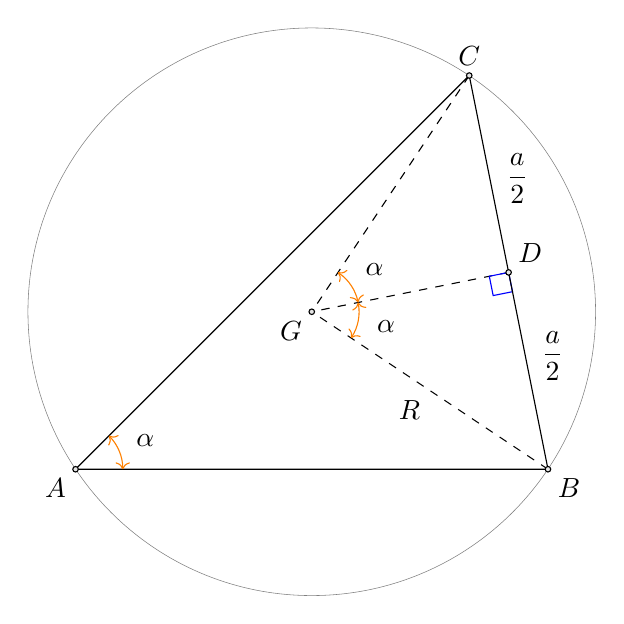
\begin{tikzpicture}[scale=1]
    \tkzDefPoint[label=below left:$A$](0,0){A}
    \tkzDefPoint[label=below right:$B$](6,0){B}
    \tkzDefPoint[label=above:$C$](5,5){C}
    
    % circumcircle
    \tkzCircumCenter(A,B,C)\tkzGetPoint{G}
    \tkzDrawCircle(G,A)
    \tkzLabelPoints[below left](G)

    \coordinate[label=above right:$D$](D) at ($(B)!(G)!(C)$);

    \draw[dashed](B)--(G) node[midway,below left]{$R$};
    \draw[dashed](C)--(G);
    \draw[dashed](D)--(G);
    \tkzMarkRightAngle[color=blue](G,D,B)
    \draw(A)--(B)--(C)
        node[pos=0.20,above right]{$\dfrac{a}2$} 
        node[pos=0.65,above right]{$\dfrac{a}2$} --cycle;

    \draw pic["$\alpha$",draw=orange,<->,angle eccentricity=1.6,angle radius=.6cm] {angle=B--A--C};
    \draw pic["$\alpha$",draw=orange,<->,angle eccentricity=1.6,angle radius=.6cm] {angle=B--G--D};
    \draw pic["$\alpha$",draw=orange,<->,angle eccentricity=1.6,angle radius=.6cm] {angle=D--G--C};

    \foreach \p in{A,B,C,D,G}{
      \tkzDrawPoint(\p)
    }
  \end{tikzpicture}    
  % Maybe due to BUG of pgfplots, there're wide space between figure
  % and caption, -3cm is measured by eye
  \vspace*{-3.5cm}
  \caption{三角形外接圆半径}
  \label{fig:R-of-circumcircle}
\end{figure}
\begin{proof}
  由图~\ref{fig:R-of-circumcircle}容易看出$\angle BAC = \angle CGD = \angle BGD$,从而有
  \begin{align*}
    S_{\triangle ABC} = \frac12 bc\cdot\sin\angle BAC
    = \frac12 bc \cdot \frac{a/2}{R} = \frac{abc}{4R}
  \end{align*}
  从而可算出$R$。
\end{proof}


\begin{theorem}
  任意$\triangle ABC$,记$a,b,c$是其三边边长,$r,R$分别是其内切圆与外接圆半径,则
  \begin{align}
    rR=\frac{abc}{2(a+b+c)}
  \end{align}
\end{theorem}
\begin{proof}
  在定理~\ref{th:R-of-circumcircle},将$r=\dfrac{S}{s}$及$a+b+c=2s$代入可得。
\end{proof}




\begin{theorem}[托勒密不等式,Ptolemy's Inequality]
  任意凸四边形$ABCD$,有
  \begin{align}
    AB\cdot CD + AD\cdot BC\ge AC\cdot BD
  \end{align}
  当且仅当$ABCD$是圆内接四边形等号成立。
\end{theorem}
\begin{proof}
  \color{red}不会呢。
\end{proof}

\begin{theorem}[鄂尔多斯—门德尔不等式,Erdos-Mordell Inequality,E-M不等式]
  $P$是三角形$ABC$内任意一点,$P$到三角形三边的距离分别为$p,q,r$,到三顶点的距离分别是$x,y,z$,则
  \begin{align}
    x+y+z\ge 2(p+q+r)
  \end{align}
\end{theorem}
\begin{proof}
  \color{red}不会呢。
\end{proof}

\section{Cauchy-Schwarz不等式}
\label{sec:cauchy-schwarz-inequalities}

% Cauchy-Schwarz
\begin{theorem}[Cauchy-Schwarz Inequality]
对 $\forall a_i, b_i\in \mathcal{R}$, $\forall n\in\mathcal{Z}^+$, 总有
\begin{align}
  \left(\sum_{i=1}^{n} a_ib_i\right)^2 \le \left(\sum_{i=1}^{n}a_i^2\right) \left(\sum_{i=1}^{n}b_i^2\right)
\end{align}
\end{theorem}

\begin{proof}
  令
  \begin{align*}
    S_n = \left(\sum_{i=1}^{n}a_i^2\right) \left(\sum_{i=1}^{n}b_i^2\right) - \left(\sum_{i=1}^{n} a_ib_i\right)^2
  \end{align*}
  则 $S_1 = a_1^2b_1^2 - (a_1b_1)^2 = 0$,且
  \begin{align*}
    S_{n+1} - S_n =& \phantom{-} \left(\sum_{i=1}^{n+1}a_i^2\right) \left(\sum_{i=1}^{n+1}b_i^2\right) - \left(\sum_{i=1}^{n+1} a_ib_i\right)^2 \\
     &- \left(\sum_{i=1}^{n}a_i^2\right) \left(\sum_{i=1}^{n}b_i^2\right) + \left(\sum_{i=1}^{n} a_ib_i\right)^2\\
  \end{align*}
  请自行证明 $S_{n+1}\ge S_n$。从而有 $S_{n+1}\ge S_n\ge\cdots S_1 = 0$。
\end{proof}

\note 令$A\equiv\left(\sum_{i=1}^{n}a_i^2\right)$, $B\equiv\left(\sum_{i=1}^{n}b_i^2\right)$,$C\equiv\left(\sum_{i=1}^{n}b_i^2\right)$,则
\begingroup\allowdisplaybreaks
\begin{align*}
  S_{n+1} - S_n &=&& (A+a_{n+1}^2)(B+b_{n+1}^2) - (C+a_{n+1}b_{n+1})^2 - AB + C^2\\
  &=&& AB + Ab_{n+1}^2 + a_{n+1}^2B + a_{n+1}^2b_{n+1}^2 - C^2 - 2a_{n+1}b_{n+1}C - a_{n+1}^2b_{n+1}^2\\
  &&&- AB + C^2\\
  &=&& Ab_{n+1}^2 + a_{n+1}^2B - 2a_{n+1}b_{n+1}C\\
  &=&& \left(\sum_{i=1}^{n}a_i^2\right) b_{n+1}^2 + \left(\sum_{i=1}^{n}b_i^2\right) a_{n+1}^2
       - \left(\sum_{i=1}^{n}a_ib_i\right) \cdot 2a_{n+1}b_{n+1}\\
  &=&& \sum_{i=1}^{n} \left( a_i^2b_{n+1}^2 + b_i^2a_{n+1}^2 - a_ib_i\cdot 2a_{n+1}b_{n+1} \right)\\
  &=&& \sum_{i=1}^{n} \left( (a_ib_{n+1})^2 + (b_ia_{n+1})^2 - 2(a_ib_{n+1})(b_ia_{n+1}) \right)\\
  &=&& \sum_{i=1}^{n} \left( (a_ib_{n+1} - b_ia_{n+1})^2 \right)\\
  &\ge&&0
\end{align*}
\endgroup


% Convex
\chapter{凸函数}
\label{chap:convex-functions}

一般英文中用Convex function和Concave function来表示凸函数与凹函数。此概念刚传入国内时,convex function被翻译为“下凹函数”,concave function被翻译成“上凸函数”,后来有些作者将其中的“下”与“上”去掉了,convex function就变成了“凹函数”,concave function就变成了“凸函数”,概念完全相反了。这就导致了有相当多的书籍中的凹凸性与concave/convex两字的含议完全相反。若阅读到此类书籍,务必要小心其定义。

%%% 未考证:
% 若你接触到经济学中的凹凸性,则可能又与数学上的定义有差别,这是因为其考虑方向不一样。数学的凹凸性是相对于$x$轴,经济学的凹凸性是相对于原点。

这里取convex/concave两词的本义,即将文献中convex function对应的称为凸函数,concave function对应的称为凹函数。

\section{凸函数的定义}
\label{sec:definition-of-convexity}

\begin{definition}[凸函数,Convex Function]\mbox{}\par
  \begin{enumerate}
  \item 函数$f(x)$被称为域$\mathcal{D}$上的凸函数,若$\forall x1,x2\in\mathcal{D}, t\in[0,1]$,下面不等式成立:
    \begin{align}\label{eq:convex-defintion}
      f\left(tx_1+(1-t)x_2\right)\le tf(x_1) + (1-t)f(x_2)
    \end{align}
  \item 函数$f(x)$被称为域$\mathcal{D}$上的严格凸函数,若$\forall x1,x2\in\mathcal{D}, t\in(0,1),x_1\ne x_2$,下面不等式成立:
    \begin{align}
      f\left(tx_1+(1-t)x_2\right)< tf(x_1) + (1-t)f(x_2)
    \end{align}
  \end{enumerate}
\end{definition}

从图形上看,凸函数对应的曲线上任意两点的连线在曲线之上。令$t\equiv 1-\lambda$代入,不等式\ref{eq:convex-defintion}还可以等价的写成以下形式
\begin{align*}
  f\left(x_1+\lambda(x_2-x_1)\right)\le f(x_1) + \lambda \left(f(x_2)-f(x_1)\right)
\end{align*}


\begin{figure}[htb]
  \centering
  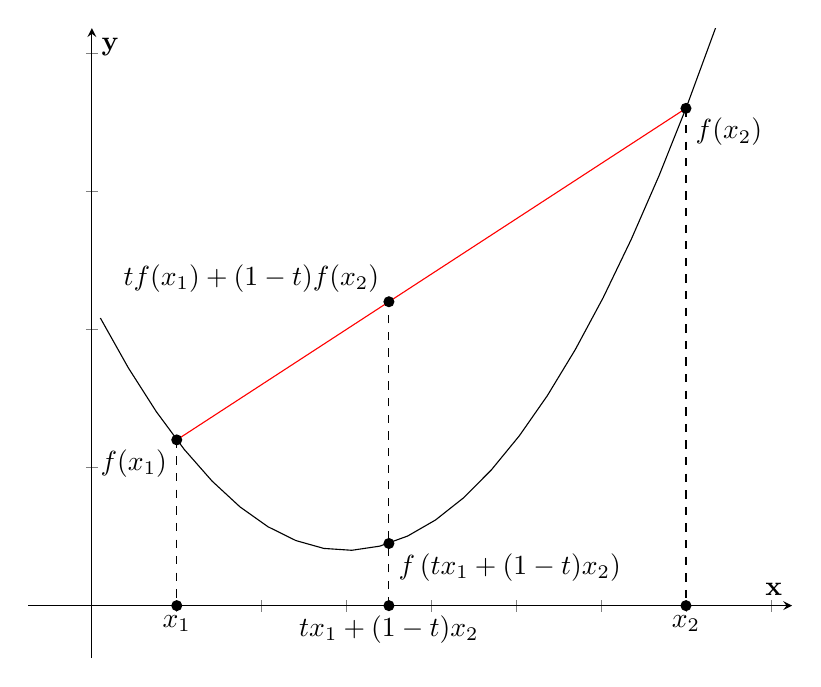
\begin{tikzpicture}[scale=1]
    \begin{axis}[
      scale only axis,
      width=0.8\textwidth,
      height=8cm,
      xmin = 0,
      xmax = 75,
      ymin = 0,
      ymax = 38, 
      axis lines = middle,
      enlargelimits = true,
      xlabel = {$\mathbf{x}$},
      ylabel = {$\mathbf{y}$},
      yticklabels={,,},
      xticklabels={,,}
      ]
      % \addplot+[mark = none] coordinates {%
      %   (0 ,40) 
      %   (20, 30)
      %   (30, 20)
      %   (35, 10)
      %   (39, 0)};
      \coordinate (A) at (axis cs:10,12);
      \coordinate (B) at (axis cs:70,36);
      \coordinate (C) at (axis cs:35,4.5);
      \coordinate (D) at (axis cs:35,22);
      \coordinate (E) at (axis cs:35,0);
      \coordinate (F) at (axis cs:10,0);
      \coordinate (G) at (axis cs:70,0);
      \addplot[domain=1:80] (\x, {0.02 * (\x * \x - 60 * \x + 900) + 4});
      \addplot[dashed](35,0)--(D);
      % \addplot[dashed](A)--(F);
      % \addplot[dashed](B)--(G);
    \end{axis}
    \draw[color=red](A)--(B);
    \fill(A) circle(2pt) node[below left] {$f(x_1)$};
    \fill(B) circle(2pt) node[below right] {$f(x_2)$};
    \fill(C) circle(2pt) node[below right] {$f\left(tx_1 + (1-t)x_2\right)$};
    \fill(D) circle(2pt) node[above left] {$tf(x_1) + (1-t)f(x_2)$};
    \fill(E) circle(2pt) node[below] {$tx_1 + (1-t)x_2$};
    \fill(F) circle(2pt) node[below] {$x_1$};
    \fill(G) circle(2pt) node[below] {$x_2$};
    \draw[dashed](A)--(F);
    \draw[dashed](B)--(G);
  \end{tikzpicture}
  \caption{凸函数}
  \label{fig:convex-function}
\end{figure}

\begin{theorem}
  若$f(x)$在$\mathcal{D}$上二次可导,那么以下条件相互等价:
  \begin{enumerate}
  \item \label{item:convex-1} $f(x)$是凸函数。
  \item \label{item:convex-2} $\forall x,y\in\mathcal{D}, f(y)\ge f(x)+f'(x)(y-x).$
  \item \label{item:convex-3} $\forall x\in\mathcal{D}, f''(x)\ge 0.$
  \end{enumerate}
\end{theorem}
\begin{proof}
  \begin{enumerate}
  \item \ref{item:convex-1}$\implies$\ref{item:convex-2}. 由于$f(x)$是凸函数,从而$\forall\lambda\in(0,1)$,有
    \begin{align*}
      &f\left(x+\lambda(y-x)\right)\le f(x)+\lambda\left(f(y)-f(x)\right)\\
      \implies & f(y)-f(x)\ge \frac{f\left(x+\lambda(y-x)\right) -  f(x)}{\lambda}\\
      \implies & f(y)-f(x)\ge \frac{f\left(x+\lambda(y-x)\right) -  f(x)}{\lambda(y-x)}\cdot(y-x)
    \end{align*}
    上式中令$\lambda\downarrow 0$,即$\Delta x\equiv\lambda(y-x)\downarrow 0$,从而有
    \begin{align*}
      f(y)-f(x)\ge \lim_{\Delta\downarrow 0}\frac{f(x+\Delta x) -  f(x)}{\Delta x}\cdot(y-x) = f'(x)(y-x)
    \end{align*}
  \item \ref{item:convex-2}$\implies$\ref{item:convex-3}.\think 请利用二阶导数定义自行证明。
  \item \ref{item:convex-3}$\implies$\ref{item:convex-1}.\think 利用中值定理自行证明。
  \end{enumerate}
  \note
  其中第\ref{item:convex-2}点说明$f$的曲线在定义域上任意一点的切线之上,
  如图~\ref{fig:convex-function-above-tangent-line}所示;
  第\ref{item:convex-3}点说明曲线的二阶导数非负,也就时说其一阶导数是单
  调增函数。
\end{proof}

\begin{figure}[htb]
  \centering
  \begin{tikzpicture}[scale=1]
    \begin{axis}[
      scale only axis,
      width=0.8\textwidth,
      height=3cm,
      xmin = 0,
      xmax = 75,
      ymin = 0,
      ymax = 27, 
      axis lines = middle,
      enlargelimits = true,
      xlabel = {$\mathbf{x}$},
      ylabel = {$\mathbf{y}$},
      yticklabels={,,},
      xticklabels={,,}
      ]
      \coordinate (A) at (axis cs:40,6);
      \addplot[domain=1:80] (\x, {0.02 * (\x * \x - 60 * \x + 900) + 4});
      \addplot[domain=10:60,color=red] (\x, {6 + 0.4 * (\x - 40)});
    \end{axis}
    \fill(A) circle(2pt) node[below left] {};
  \end{tikzpicture}
  \caption{凸函数示意:曲线位于任一点的切线之上}
  \label{fig:convex-function-above-tangent-line}
\end{figure}


% Jensen
\begin{theorem}
  如果$f(x)$是凸函数,那么对于$p_i\ge0$且$\sum_{i=1}^{n}p_i=1$,有
  \begin{align}
    f(\sum_{i=1}^{n}p_ix_i)\le \sum_{i=1}^{n}p_i f(x_i)
  \end{align}
\end{theorem}

\begin{proof}
  事实上,Jensen不等式与凸函数的定义是等价的,即若函数$f(x)$是凸函数,
  当且仅当$f(x)$满足Jensen不等式。
  \begin{enumerate}
  \item 充分性。在Jensen不等式中令$n=2$,可知$f(x)$满足凸函数定义,从而是凸函数。
  \item 必要性。设$f(x)$是凸函数,$n=2$时Jensen不等式即是凸函数定义中的条件,即Jensen不等式在$n=2$时成立。
    设Jensen不等式对$n\le K$时成立,考虑$n=K+1$的情况。关键点,把其中两项凑成一项,从而$K+1$项变成$K$项,可利用$n\le K$时成立的结论。令
    \begin{align*}
      p_K'&\equiv p_K+p_{K+1}\\
      x_K'&\equiv\frac{p_K}{p_K'}x_K + \frac{p_{K+1}}{p_K'}x_{K+1}\in[\min{(x_K, x_{K+1})}, \max{(x_K, x_{K+1})}]
    \end{align*}
    则有$p_K'x_K' = p_Kx_K + p_{K+1}x_{K+1}$,且
    \begin{align*}
      f\left(\sum_{i=1}^{K+1}p_ix_i\right) &= f\left(\sum_{i=1}^{K-1}p_ix_i  + p_K'x_K'\right)\\
      &\le \left(\sum_{i=1}^{K-1}p_if(x_i)\right) + p_K' f(x_K')\\
      &\le \left(\sum_{i=1}^{K-1}p_if(x_i)\right) + p_K'\left( \frac{p_K}{p_K'}f(x_K) + \frac{p_{K+1}}{p_K'}f(x_{K+1}) \right) \\
      &= \left(\sum_{i=1}^{K+1}p_i f(x_i)\right)
    \end{align*}
    此处没有考虑$p_K'=0$的情况,请自行补充完整。
  \end{enumerate}
  
  \note $p_K'$和$x_K'$是如何凑出来的?令$p_K'x_K' = p_Kx_K + p_{K+1}x_{K+1}$,
  且$p_K'$需满足$\sum_{i=1}^{K-1}p_i + p_K'=1$,从而可得。
\end{proof}

{\color{red}下面这个是对的吗?}
\begin{theorem}
  $f(x)$是$\mathcal{D}$上的严格凸函数,当且仅当对$\forall n\in\mathcal{Z}^+, x_i\in\mathcal{D}, p_i>0, \sum_{i=1}^{n}p_i=1$,以下不等式成立:
  \begin{align*}
    f\left(\sum_{i=1}^{n} p_i x_i\right) < \sum_{i=1}^{n} p_i f(x_i)
  \end{align*}
\end{theorem}


\begin{lemma}\label{lemma:convexity-extension}
  若$f(x)$是$[a,b]$上的连续函数,且在$(a,b]$上是凸的,则$f(x)$在$[a,b]$上是凸函数。
\end{lemma}
\begin{proof}
  下面按定义证明,即$\forall x_1,x_2\in[a,b], 0\le t\le1$,需要证明
  \begin{align*}
    f\left(tx_1 + (1-t)x_2\right) \le tf(x_1) + (1-t)f(x_2)
  \end{align*}
  若$x_1$和$x_2$都不等于$a$,那么由条件$f(x)$在$(a,b]$上严格凸可知上面不等式成立。下面不妨设$a=x_1<x_2\le b$。由连续性,可取到序列$c_i$,使得$\forall i, a=x_1<c_i\le b$,且$\lim c_i = x_1$,从而对于$c_i$和$x_2$,有
  \begin{align*}
    f\left(tc_i + (1-t)x_2\right) \le tf(c_i) + (1-t)f(x_2)
  \end{align*}
  上式中两边对$i$取极限,并由$f(x)$的连续性,有
  \begin{align*}
    \lim_{i\to\infty}f\left(tc_i + (1-t)x_2\right) &\le \lim_{i\to\infty} tf(c_i) + (1-t)f(x_2)\\
    f\left(\lim_{i\to\infty}\left(tc_i + (1-t)x_2\right)\right) &\le tf( \lim_{i\to\infty} c_i) + (1-t)f(x_2)\\
    f\left(tx_1 + (1-t)x_2\right) &\le tf(x_1) + (1-t)f(x_2)
  \end{align*}
\end{proof}

\think 上面引理对严格凸函数是否还能保持严格凸性?

\begin{lemma}\label{lemma:convexity-of-power-function}
  对$p>1$,函数$f(x)\equiv\left|x\right|^p$在$x\in\mathcal{R}$上是严格凸函数。
\end{lemma}
\begin{proof}
  函数$f(x)\equiv|x|^p$的凹凸性在图形上看是非常明显的。

  使用导数的概念证明也是非常明显的,分段考虑,$\forall x>0, f'(x) = p\left|x\right|^{p-1}>0, f''(x)=p(p-1)\left|x\right|^{(p-1)(p-2)}>0$,从而$f(x)$的一阶导数是严格单调递增的,从而$f(x)$在$(0,+\infty)$上是凸函数。同样$f(x)$在$(-\infty,0)$上也是凸函数。

  下面是初等数学的证明。

  $\forall x_1\le x_2, t\in(0,1)$,有
  \begin{align*}
    f\left(tx_1 + (1-t)x_2\right) = \left|tx_1 + (1-t)x_2\right|^p
  \end{align*}
  {\color{red}然后呢??}
\end{proof}

下面是Jensen不等式的另一种形式。
\begin{theorem}[Jensen不等式]
  若$f$是$\mathcal{D}$上的凸函数,且$\forall x_1,x_2,\cdots,x_n\in\mathcal{D}$,则
  \begin{align}
    f\left(\frac{x_1+x_2+\cdots+x_n}{n}\right)\le\frac{f(x_1)+f(x_2)+\cdots+f(x_n)}{n}
  \end{align}
  若$f$还是严格凸的,则当且仅当$x_1=x_2=\cdots=x_n$时等号成立。
\end{theorem}

\begin{proof}
  {\color{red}请证明两种形式的Jensen不等式是等价的。}
\end{proof}

\begin{example}
  对$\triangle ABC$,证明:
  \begin{align*}
    \sin A + \sin B + \sin C \le \frac{3\sqrt3}{2}
  \end{align*}
  且说明等号在何时成立。
\end{example}

\begin{proof}
  $f(x)\equiv\sin(x)$在$[0,\pi]$上是严格凹函数,由Jensen不等式有
  \begin{align*}
    \sin A + \sin B + \sin C \le 3\sin\frac{A+B+C}{3} = \frac{3\sqrt3}{2}
  \end{align*}
  当且仅当$A=B=C$时,即$A=B=C=\frac\pi3$时等号成立。
\end{proof}

\begin{example}
  若$a,b,c$是和为1的正数,求下式的最小值
  \begin{align*}
    \left(a+\frac1a\right)^{10} + 
    \left(b+\frac1b\right)^{10} + 
    \left(c+\frac1c\right)^{10}
  \end{align*}
\end{example}

\begin{proof}
  首先证明以下函数在$(0,1)$上是严格凸函数({\color{red}请用二次导数自行证明})
  \begin{align*}
    f(x)\equiv\left(x+\frac1x\right)^{10}
  \end{align*}
  其次利用Jensen不等式,有
  \begin{align*}
    &\left(a+\frac1a\right)^{10} + 
    \left(b+\frac1b\right)^{10} + 
    \left(c+\frac1c\right)^{10}\\
    ={}  & f(a) + f(b) + f(c)\\
    \ge{}& 3f\left(\frac{a+b+c}3\right)\\
    ={}  & 3f\left(\frac\13\right) = 3 \left(\frac{10}{3}\right)^{10} = \frac{10^{10}}{3^9}
  \end{align*}
  当且仅当$a=b=c=\frac13$时等号成立。
\end{proof}
% Minkowski Inequality

\chapter{Minkowski不等式}
\label{chap:minkowski-inequality}


\begin{theorem}[Minkowski不等式]
  $\forall p\ge 1$以下不等式对任意$x_i,y_i\in\mathcal{R}$成立:
  \begin{align}
    \left(\sum_{i=1}^{n}\left|x_i+y_i\right|^p\right)^\frac{1}{p}
    \le
    \left(\sum_{i=1}^{n}\left|x_i\right|^p\right)^\frac{1}{p}
    +
    \left(\sum_{i=1}^{n}\left|y_i\right|^p\right)^\frac{1}{p}
  \end{align}
  当且仅当存在不同时为零的常数$\alpha,\beta$,$\alpha x_i=\beta
  y_i$对$\forall i\in\{1,2,\cdots,n\}$都成立时等号成立。即若记
  \begin{align*}
    \vec{x}&\equiv\left[x_1,x_2,\cdots,x_n\right]\\
    \vec{y}&\equiv\left[y_1,y_2,\cdots,y_n\right]
  \end{align*}
  则当且仅当 $\vec{x}$ 和 $\vec{y}$ 线性相关时等号成立。
\end{theorem}

Minkowski不等式与函数的凸性相关。

\begin{proof}
  当$p=1$时显然不等式成立。下面考虑$p>1$的情况。由引理\ref{lemma:convexity-of-power-function},$|x|^p$是凸函数,$|x|^{\frac{1}{p}}$是凹函数,从而$\forall t\in(0,1)$,有
  \begin{align*}
    \left|x_i + y_i\right|^p &= \left|t\cdot\frac{x_i}{t} + (1-t)\cdot\frac{y_i}{1-t}\right|^p & \forall t\in (0,1)\\
    &\le t \left|\frac{x_i}{t}\right|^p + (1-t)\left|\frac{y_i}{1-t}\right|^p \\
    &= t^{1-p}|x_i|^p + (1-t)^{1-p}|y_i|^p
  \end{align*}
  求和,则有
  \begin{align*}
    \sum_{i=1}^{n}\left|x_i+y_i\right|^p \le
    t^{1-p}\sum_{i=1}^{n}|x_i|^p + (1-t)^{1-p}\sum_{i=1}^{n}|y_i|^p
  \end{align*}
  记
  \begin{align*}
    \norm{X}  \equiv\left(\sum_{i=1}^{n} |x_i|^p\right)^{\frac1p},\quad
    \norm{Y}  \equiv\left(\sum_{i=1}^{n} |y_i|^p\right)^{\frac1p},\quad
    \norm{X+Y}\equiv\left(\sum_{i=1}^{n} |x_i+y_i|^p\right)^{\frac1p}
  \end{align*}
  并令$t\equiv\frac{\norm{X}}{\norm{X}+\norm{Y}}$(显然 $t\in[0,1]$ 。
  若$t=0$或者$t=1$,则$\norm{X}=0$或者$\norm{Y}=0$,从而Minkowski等号成
  立,所以下面只考虑$t\in(0,1)$的情况),代入则有
  \begin{align*}
    \norm{X + Y}^p &= \sum_{i=1}^{n}\left|x_i+y_i\right|^p\\
    &\le t^{1-p}\sum_{i=1}^{n}|x_i|^p + (1-t)^{1-p}\sum_{i=1}^{n}|y_i|^p\\
    &= \left(\frac{\norm{X}}{\norm{X}+\norm{Y}}\right)^{1-p} \norm{X}^p +
      \left(\frac{\norm{Y}}{\norm{X}+\norm{Y}}\right)^{1-p} \norm{Y}^p\\
    &=\frac{\norm{X}+\norm{Y}}{\left(\norm{X}+\norm{Y}\right)^{1-p}}\\
    &= \left(\norm{X}+\norm{Y}\right)^{p}
  \end{align*}
  从而有$\norm{X+Y}\le\norm{X}+\norm{Y}$,即Minkowski不等式成立。
\end{proof}


\chapter{函数图形}
\label{chap:graphs-of-functions}

\section{基本函数}
\label{sec:graphs-of-basic-functions}

\begin{itemize}
\item 一元一次函数

\begin{center}
  \begin{tikzpicture}[scale=1.0]
    \begin{scope}[shift={(0,0)}]
      \draw[|<->](-2,-.5)--(0,-.5)node[midway,below]{$\dfrac ba$};
      \draw[|<->](.5,1)--(.5,0)node[midway,right]{$b$};
      % \node[below] at (0,-2) {$y=ax+b$};
      \draw[->](-4,0)--(4,0) node[below]{$x$};
      \draw[->](0,-1)--(0,3) node[left]{$y$};
      \draw[very thick](-4,-1)--(4,3) node[below,right]{$f(x)=ax+b$};
    \end{scope}
  \end{tikzpicture}
\end{center}

\item 一元二次函数,其一般表达式(配方后)为
\begin{align*}
  f(x)=a\left(x+b\right)^2+c
\end{align*}
其对称轴为$x=-b$,唯一极值点为$(-b,c)$。
\begin{center}
  \begin{tikzpicture}[scale=2.0]
    \begin{scope}[shift={(0,0)}]
      \draw[->](-2,0)--(2,0) node[below]{$x$};
      \draw[->](0,-1)--(0,1.5) node[left]{$y$};
      \draw[dashed](.25,-1)--(.25,1.5) node[pos=0,right]{$x=-b$};
      \draw[dashed](-2,-.625)--(2,-.625) node[below]{$y=c$};
      \draw[very thick,domain=-.75:1.25,smooth,variable=\x]plot({\x},{2*\x*\x - \x - .5});
    \end{scope}
  \end{tikzpicture}
\end{center}

\item 三次方函数
\begin{center}
  \begin{tikzpicture}[scale=.5]
    \begin{scope}[shift={(0,0)}]
      \draw[->](-6,0)--(6,0) node[below]{$x$};
      \draw[->](0,-8)--(0,8) node[left]{$y$};
      \draw[very thick,domain=-2:2,smooth,variable=\x]plot({\x},{\x*\x*\x});
      \node[below right] at(1,1){$f(x)=x^3$};
    \end{scope}
  \end{tikzpicture}
\end{center}

\item 平方根函数
\begin{center}
  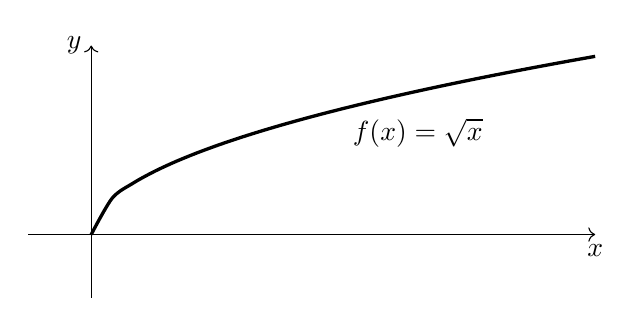
\begin{tikzpicture}[scale=.8]
    \begin{scope}[shift={(0,0)}]
      \draw[->](-1,0)--(8,0) node[below]{$x$};
      \draw[->](0,-1)--(0,3) node[left]{$y$};
      \draw[very thick,domain=0:8,smooth,variable=\x]plot({\x},{sqrt(\x)});
      \node[below right] at(4,2){$f(x)=\sqrt x$};
    \end{scope}
  \end{tikzpicture}
\end{center}

\item 绝对值函数
\begin{align*}
  f(x)=\left|x\right|=
  \begin{cases}
    -x,&\quad x<0\\
    \phantom{-}x,&\quad x\ge 0
  \end{cases}
\end{align*}
\begin{center}
  \begin{tikzpicture}[scale=1]
    \begin{scope}[shift={(0,0)}]
      \draw[->](-3,0)--(3,0) node[below]{$x$};
      \draw[->](0,-1)--(0,3.5) node[left]{$y$};
      \draw[very thick](-3,3)--(0,0)--(3,3) node[below right]{$f(x)=\left|x\right|$};
    \end{scope}
  \end{tikzpicture}
\end{center}

\item 倒数函数
\begin{center}
  \begin{tikzpicture}[scale=1]
    \begin{scope}[shift={(0,0)}]
      \draw[->](-3,0)--(3,0) node[below]{$x$};
      \draw[->](0,-3)--(0,3) node[left]{$y$};
      \draw[very thick,domain=.35:2.5,smooth,variable=\x]plot({\x},{1/\x});
      \draw[very thick,domain=-2.5:-.35,smooth,variable=\x]plot({\x},{1/\x});
      \node[right]at(1.1,1.5){$f(x)=\dfrac1x$};
    \end{scope}
  \end{tikzpicture}
\end{center}
\end{itemize}



\chapter{无字证明}
\label{chap:proofs-without-words}

\epigraph{一图胜千言,一表胜万卷。}{}

无字证明(Proof without Words)是指仅用图像而无需文字解释就能不证自明的数学命题。然而无字证明并不是严格的数学证明,只是帮助直观理解。

\section{代数}
\label{sec:pww-algebra}

\begin{example}
  前$n$个奇数的和等于$n^2$,即
  \begin{align}
    \underbrace{1 + 3 + 5 + \cdots + (2n-1)}_{n\text{个}} = n^2
  \end{align}
\end{example}

\begin{center}
  \begin{tikzpicture}[scale=0.6]
    \begin{scope}[shift={(0,0)}]
      \foreach \r/\f in{1/white,2/red!30,3/white,4/blue!30,5/white,6/violet!30}{
        \draw[fill=\f](-\r,-\r) rectangle(\r-1,1-\r);
        \draw(-\r,-\r)grid(\r-1,1-\r);
        \draw[pattern=north east lines, pattern color=black](-1,-\r) rectangle(0,1-\r);
      }    
    \end{scope}
    \begin{scope}[shift={(7,0)}]
      \draw[|<->|](0,0)--(0,-6) node[midway,fill=white]{$n$层};
    \end{scope}
    \begin{scope}[shift={(9,0)}]
      \foreach \r/\f in{1/white,2/red!30,3/white,4/blue!30,5/white,6/violet!30}{
        \draw[fill=\f](0,-\r) rectangle(\r,1-\r);
        \draw(0,-\r)grid(\r,1-\r);
        \draw[fill=\f](\r,0) rectangle(\r-1,-\r);
        \draw(\r,0) grid(\r-1,-\r);
        \draw[pattern=north east lines, pattern color=black](\r-1,1-\r) rectangle(\r,-\r);
      }
    \end{scope}
  \end{tikzpicture}
\end{center}

\begin{example}
  前$n$个数的和是$\dfrac{(n+1)}{2}$,即
  \begin{align}
    1+2+3+\cdots+n=\frac{n(n+1)}{2}
  \end{align}
\end{example}
\begin{center}
  \begin{tikzpicture}[scale=0.6]
    \begin{scope}[shift={(0,0)}]
      \foreach \r/\f in{1/white,2/red!30,3/white,4/blue!30,5/white,6/violet!30}{
        \draw[fill=\f](0,1-\r) rectangle(\r, -\r);
        \draw(0,1-\r) grid(\r, -\r);
      }    
    \end{scope}
    \begin{scope}[shift={(8,0)}]
      \draw[|<->|](0,0)--(0,-6) node[midway,fill=white]{$n$层};
    \end{scope}
    \begin{scope}[shift={(10,0)}]
      \foreach \r/\f in{1/white,2/red!30,3/white,4/blue!30,5/white,6/violet!30}{
        \draw[fill=\f](0,1-\r) rectangle(\r, -\r);
        \draw(0,1-\r) grid(\r, -\r);
      }
      \foreach \r/\f in{1/violet!30,2/white,3/blue!30,4/white,5/red!30,6/white}{
        \draw[fill=\f](\r,1-\r) rectangle(7, -\r);
        \draw(\r,1-\r) grid(7, -\r);
      }
      \draw[very thick](1,0)--(1,-1)--(2,-1)--(2,-2)--(3,-2)--(3,-3)
                     --(4,-3)--(4,-4)--(5,-4)--(5,-5)--(6,-5)--(6,-6);
      \draw[|<->|](0,-7)--(7,-7) node[midway,fill=white]{$n+1$};      
    \end{scope}
  \end{tikzpicture}
\end{center}

\begin{example}
  \begin{align*}
    1+2+3+\cdots+(n-1)=\binom n2
  \end{align*}
  \begin{center}
    \begin{tikzpicture}[scale=1.0]
      \begin{scope}[shift={(0,0)}]
        \foreach \x/\y in {
          0/0,
          -.6/-1,.6/-1,
          -1.2/-2,0/-2,1.2/-2,
          -1.8/-3,-.6/-3,.6/-3,1.8/-3,
          -2.4/-4,-1.2/-4,0/-4,1.2/-4,2.4/-4,
          -3.0/-5,-1.8/-5,-.6/-5,.6/-5,1.8/-5,3.0/-5
          }{
            \draw[fill=yellow!30](\x,\y)circle(.5);
          }
          \foreach \x/\y in {
            -3.6/-6,-2.4/-6,-1.2/-6,0/-6,1.2/-6,2.4/-6,3.6/-6
          }{
            \draw[pattern=north west lines](\x,\y)circle(.5);
          }
          \draw[->](.6,-3)--(-1.2,-6);
          \draw[->](.6,-3)--(2.4,-6);
      \end{scope}
    \end{tikzpicture}
  \end{center}

  如图,在$7$个带阴影的圆中选$2$个,每种选法与其上某个圆圈一一对应,即三个圆圆心组成一个等腰三角形。
\end{example}

\pagebreak
\newcommand{\fixedcirclenode}[3]{\draw #1 circle(#2) node {#3};}
\begin{example}
  \begin{align*}
    1^2+2^2+3^2+\cdots=\frac{n(n+1)(2n+1)}6
  \end{align*}
  \centering
  \begin{tikzpicture}[scale=.6]
    \begin{scope}[shift={(0,0)}]
      \fixedcirclenode{(0,0)}{.5}{1};
      \fixedcirclenode{(-.5,-1)}{.5}{2}; \fixedcirclenode{(.5,-1)}{.5}{2};
      \fixedcirclenode{(-1,-2)}{.5}{3};  \fixedcirclenode{(0,-2)}{.5}{3};  \fixedcirclenode{(1,-2)}{.5}{3}; 
      \fixedcirclenode{(-1.5,-3)}{.5}{4};  \fixedcirclenode{(-.5,-3)}{.5}{4};  \fixedcirclenode{(.5,-3)}{.5}{4}; \fixedcirclenode{(1.5,-3)}{.5}{4}; \fixedcirclenode{(-2,-4)}{.5}{$\cdots$};
      \fixedcirclenode{(-1,-4)}{.5}{$\cdots$};  \fixedcirclenode{(0,-4)}{.5}{$\cdots$}; \fixedcirclenode{(1,-4)}{.5}{$\cdots$}; \fixedcirclenode{(2,-4)}{.5}{$\cdots$}; 
      \fixedcirclenode{(-2.5,-5)}{.5}{$n$}; \fixedcirclenode{(-1.5,-5)}{.5}{$n$};  \fixedcirclenode{(-.5,-5)}{.5}{$\cdots$};  \fixedcirclenode{(.5,-5)}{.5}{$\cdots$}; \fixedcirclenode{(1.5,-5)}{.5}{$n$}; \fixedcirclenode{(2.5,-5)}{.5}{$n$}; 
    \end{scope}
    
    \begin{scope}[shift={(3.5,0)}]
      \node at (0,-2) {{\huge $+$}};
    \end{scope}

    \begin{scope}[shift={(7,0)}]
      \fixedcirclenode{(0,0)}{.5}{$n$};
      \fixedcirclenode{(-.5,-1)}{.5}{$\cdots$}; \fixedcirclenode{(.5,-1)}{.5}{$n$};
      \fixedcirclenode{(-1,-2)}{.5}{4};  \fixedcirclenode{(0,-2)}{.5}{$\cdots$};  \fixedcirclenode{(1,-2)}{.5}{$\cdots$}; 
      \fixedcirclenode{(-1.5,-3)}{.5}{3}; \fixedcirclenode{(-.5,-3)}{.5}{4}; \fixedcirclenode{(.5,-3)}{.5}{$\cdots$}; \fixedcirclenode{(1.5,-3)}{.5}{$\cdots$}; 
      \fixedcirclenode{(-2,-4)}{.5}{2};  \fixedcirclenode{(-1,-4)}{.5}{3};  \fixedcirclenode{(0,-4)}{.5}{4}; \fixedcirclenode{(1,-4)}{.5}{$\cdots$}; \fixedcirclenode{(2,-4)}{.5}{$n$}; 
      \fixedcirclenode{(-2.5,-5)}{.5}{1}; \fixedcirclenode{(-1.5,-5)}{.5}{2};  \fixedcirclenode{(-.5,-5)}{.5}{3};  \fixedcirclenode{(.5,-5)}{.5}{4}; \fixedcirclenode{(1.5,-5)}{.5}{$\cdots$}; \fixedcirclenode{(2.5,-5)}{.5}{$n$}; 
    \end{scope}

    \begin{scope}[shift={(10.5,0)}]
      \node at (0,-2) {{\huge $+$}};
    \end{scope}
    
    \begin{scope}[shift={(14,0)}]
      \fixedcirclenode{(0,0)}{.5}{$n$};
      \fixedcirclenode{(-.5,-1)}{.5}{$n$}; \fixedcirclenode{(.5,-1)}{.5}{$\cdots$};
      \fixedcirclenode{(-1,-2)}{.5}{$\cdots$}; \fixedcirclenode{(0,-2)}{.5}{$\cdots$};  \fixedcirclenode{(1,-2)}{.5}{4}; 
      \fixedcirclenode{(-1.5,-3)}{.5}{$\cdots$};  \fixedcirclenode{(-.5,-3)}{.5}{$\cdots$};  \fixedcirclenode{(.5,-3)}{.5}{4}; \fixedcirclenode{(1.5,-3)}{.5}{3};
      \fixedcirclenode{(-2,-4)}{.5}{$n$};  \fixedcirclenode{(-1,-4)}{.5}{$\cdots$};  \fixedcirclenode{(0,-4)}{.5}{4}; \fixedcirclenode{(1,-4)}{.5}{3}; \fixedcirclenode{(2,-4)}{.5}{2}; 
      \fixedcirclenode{(-2.5,-5)}{.5}{$n$}; \fixedcirclenode{(-1.5,-5)}{.5}{$\cdots$};  \fixedcirclenode{(-.5,-5)}{.5}{4};  \fixedcirclenode{(.5,-5)}{.5}{3}; \fixedcirclenode{(1.5,-5)}{.5}{2}; \fixedcirclenode{(2.5,-5)}{.5}{1}; 
    \end{scope}
  \end{tikzpicture}

  \vspace*{2cm}
  \begin{tikzpicture}[scale=1.4]
    \node at (-3,-2) {{\huge $=$}};
    \begin{scope}[shift={(0,0)}]
      \fixedcirclenode{(0,0)}{.5}{$2n+1$};
      \fixedcirclenode{(-.5,-1)}{.5}{$2n+1$}; \fixedcirclenode{(.5,-1)}{.5}{$2n+1$};
      \fixedcirclenode{(-1,-2)}{.5}{$2n+1$};  \fixedcirclenode{(0,-2)}{.5}{$2n+1$};  \fixedcirclenode{(1,-2)}{.5}{$2n+1$}; 
      \fixedcirclenode{(-1.5,-3)}{.5}{$2n+1$};  \fixedcirclenode{(-.5,-3)}{.5}{$2n+1$};  \fixedcirclenode{(.5,-3)}{.5}{$2n+1$}; \fixedcirclenode{(1.5,-3)}{.5}{$2n+1$}; \fixedcirclenode{(-2,-4)}{.5}{$\cdots$};
      \fixedcirclenode{(-1,-4)}{.5}{$\cdots$};  \fixedcirclenode{(0,-4)}{.5}{$\cdots$}; \fixedcirclenode{(1,-4)}{.5}{$\cdots$}; \fixedcirclenode{(2,-4)}{.5}{$\cdots$}; 
      \fixedcirclenode{(-2.5,-5)}{.5}{$2n+1$}; \fixedcirclenode{(-1.5,-5)}{.5}{$2n+1$};  \fixedcirclenode{(-.5,-5)}{.5}{$\cdots$};  \fixedcirclenode{(.5,-5)}{.5}{$\cdots$}; \fixedcirclenode{(1.5,-5)}{.5}{$2n+1$}; \fixedcirclenode{(2.5,-5)}{.5}{$2n+1$}; 
    \end{scope}
  \end{tikzpicture}
  \begin{align*}
    \text{从而有}\quad 3\left(1^2+2^2+3^2+\cdots+n^2\right) = (2n+1)\cdot \frac{n(n+1)}2
  \end{align*}
\end{example}

\pagebreak
\begin{example}[维维亚尼定理,Viviani's Theorem]
  记等边三角形的高为$h$,三角形内任意一点$P$到三边的距离分别为$l,m,n$,则
  \begin{align}
    h=l+m+n
  \end{align}
\end{example}
\begin{center}
  \begin{tikzpicture}[scale=1]
    \tkzDefPoint[label=below left:$A$](0,0){A}
    \tkzDefPoint[label=below right:$B$](6,0){B}
    \tkzDefPoint[label=above:$C$](60:6){C} %polar coordinate
    \tkzDefPoint[label=below left:$P$](35:4){P}
    \coordinate(D) at ($(B)!(P)!(C)$);
    \coordinate(E) at ($(C)!(P)!(A)$);
    \coordinate(F) at ($(A)!(P)!(B)$);

    \coordinate(Q) at (0,6);
    \coordinate(C'') at ($(A)!(C)!(Q)$);
    \coordinate(P'') at ($(A)!(P)!(Q)$);
    \coordinate(MN) at($(P) + (120:6)$);
    \tkzInterLL(P,MN)(A,C)\tkzGetPoint{M};
    \tkzInterLL(P,MN)(A,B)\tkzGetPoint{N};
    \tkzInterLL(P,MN)(C,C'')\tkzGetPoint{C'};
    \tkzInterLL(P,P'')(A,C)\tkzGetPoint{P'};
    
    \coordinate(M'') at($(A)!(M)!(Q)$);

    % the altitude
    \coordinate(H) at (-1,0);
    \coordinate(H') at (-1,6);
    \coordinate(H'') at ($(H)!(C)!(H')$);
    \draw[|<->|](H)--(H'') node[midway,fill=white]{$h$};

    \tkzMarkRightAngle[color=blue](B,D,P)
    \tkzMarkRightAngle[color=blue](C,E,P)
    \tkzMarkRightAngle[color=blue](A,F,P)

    \tkzDrawPoints(A,B,C,P,D,E,F,C',C'',P',P'',M,M'',N);
    \tkzLabelPoints[above](C')

    \draw[very thick](A)--(B)--(C)--cycle;
    \draw(P)--(D) node[pos=0.45,above]{$l$}
         (P)--(E) node[pos=0.7, below]{$m$}
         (P)--(F) node[midway, left]{$n$}
         (A)--(P'') node[midway, left]{$n$}
         (P'')--(M'') node[midway,left]{$m$}
         (M'')--(C'') node[midway,left]{$l$};
    \draw[dashed](P)--(P'') (M)--(M'') (C)--(C'') (N)--(C');
    \tkzMarkRightAngle[color=blue](P,P'',A)
    \tkzMarkRightAngle[color=blue](M,M'',A)
    \tkzMarkRightAngle[color=blue](C,C'',A)
    \tkzMarkRightAngle[color=blue](Q,A,B)

    \draw[red,thick](P)--(P')--(C)--(C')--cycle;
  \end{tikzpicture}
\end{center}

\begin{center}
  \begin{tikzpicture}[scale=.7]
    \begin{scope}[shift={(0,0)}]
      \tkzDefPoint(0,0){A}
      \tkzDefPoint(6,0){B}
      \tkzDefPoint(60:6){C} %polar coordinate
      \tkzDefPoint(35:4){P}
      \coordinate(D) at ($(B)!(P)!(C)$);
      \coordinate(E) at ($(C)!(P)!(A)$);
      \coordinate(F) at ($(A)!(P)!(B)$);
      
      \coordinate(F1) at ($(P)!sqrt(4/3)!30:(F)$);
      \coordinate(F2) at ($(P)!sqrt(4/3)!-30:(F)$);

      \coordinate(E1) at ($(P)!sqrt(4/3)!30:(E)$);
      \coordinate(E2) at ($(P)!sqrt(4/3)!-30:(E)$);

      \coordinate(D1) at ($(P)!sqrt(4/3)!30:(D)$);
      \coordinate(D2) at ($(P)!sqrt(4/3)!-30:(D)$);
      
      \coordinate(O) at ($1/3*(P)+1/3*(E1)+1/3*(E2)$);
      \calcLength(O,E1){r}
      \centerarc[->](O)(75:-15:\r pt);
      \centerarc[->](O)(-45:-135:\r pt);
      \centerarc[->](O)(-165:-255:\r pt);

      \draw[fill=red!30] (P)--(F1)--(F2)--cycle;
      \draw[fill=violet!30] (P)--(D1)--(D2)--cycle;
      \draw[fill=blue!30]  (P)--(E1)--(E2)--cycle;
      \draw (A)--(B)--(C)--cycle;
      \draw[very thick] (P)--(D) (P)--(E) (P)--(F);
    \end{scope}
    \begin{scope}[shift={(6.5,3)}]
      \node at (0,0) {\huge $\implies$};
    \end{scope}
    \begin{scope}[shift={(7,0)}]
      \tkzDefPoint(0,0){A}
      \tkzDefPoint(6,0){B}
      \tkzDefPoint(60:6){C} %polar coordinate
      \tkzDefPoint(35:4){P}
      \coordinate(D) at ($(B)!(P)!(C)$);
      \coordinate(E) at ($(C)!(P)!(A)$);
      \coordinate(F) at ($(A)!(P)!(B)$);
      
      \coordinate(F1) at ($(P)!sqrt(4/3)!30:(F)$);
      \coordinate(F2) at ($(P)!sqrt(4/3)!-30:(F)$);

      \coordinate(E1) at ($(P)!sqrt(4/3)!30:(E)$);
      \coordinate(E2) at ($(P)!sqrt(4/3)!-30:(E)$);

      \coordinate(D1) at ($(P)!sqrt(4/3)!30:(D)$);
      \coordinate(D2) at ($(P)!sqrt(4/3)!-30:(D)$);

      \coordinate(E') at ($(E2)!(E1)!(P)$);
      
      \draw[fill=red!30] (P)--(F1)--(F2)--cycle;
      \draw[fill=violet!30] (P)--(D1)--(D2)--cycle;
      \draw[fill=blue!30]  (P)--(E1)--(E2)--cycle;
      \draw (A)--(B)--(C)--cycle;
      \draw[very thick] (P)--(D) (E1)--(E') (P)--(F);

      \coordinate(O) at ($1/3*(C)+1/3*(E1)+1/3*(D2)$);
      \calcLength(O,E1){r}
      \centerarc[->](O)(75:-15:\r pt);
      \centerarc[->](O)(-45:-135:\r pt);
      \centerarc[->](O)(-165:-255:\r pt);
    \end{scope}
    \begin{scope}[shift={(13.5,3)}]
      \node at (0,0) {\huge $\implies$};
    \end{scope}
    \begin{scope}[shift={(14,0)}]
      \tkzDefPoint(0,0){A}
      \tkzDefPoint(6,0){B}
      \tkzDefPoint(60:6){C} %polar coordinate
      \tkzDefPoint(35:4){P}
      \coordinate(D) at ($(B)!(P)!(C)$);
      \coordinate(E) at ($(C)!(P)!(A)$);
      \coordinate(F) at ($(A)!(P)!(B)$);
      
      \coordinate(F1) at ($(P)!sqrt(4/3)!30:(F)$);
      \coordinate(F2) at ($(P)!sqrt(4/3)!-30:(F)$);

      \coordinate(E1) at ($(P)!sqrt(4/3)!30:(E)$);
      \coordinate(E2) at ($(P)!sqrt(4/3)!-30:(E)$);

      \coordinate(D1) at ($(P)!sqrt(4/3)!30:(D)$);
      \coordinate(D2) at ($(P)!sqrt(4/3)!-30:(D)$);

      \coordinate(E') at ($(E2)!(E1)!(P)$);
      
      \draw[fill=red!30] (P)--(F1)--(F2)--cycle;
      \draw (A)--(B)--(C)--cycle;
      \draw[very thick] (P)--(F);
      \draw (C)--(E1)--(D2)--cycle;

      \coordinate(O) at ($1/3*(C)+1/3*(E1)+1/3*(D2)$);
      \coordinate(P) at ($(O)!1!-120:(P)$);
      \coordinate(D1) at ($(O)!1!-120:(D1)$);
      \coordinate(D2) at ($(O)!1!-120:(D2)$);
      \coordinate(D)  at ($(O)!1!-120:(D)$);
      \coordinate(E1) at ($(O)!1!-120:(E1)$);
      \coordinate(E2) at ($(O)!1!-120:(E2)$);
      \coordinate(E') at ($(O)!1!-120:(E')$);
      % \draw(C)--(O);
      % \begin{scope}[rotate around={-60:(O)}]
        \draw[rotate around={-120:(O)},fill=violet!30] (P)--(D1)--(D2)--cycle;
        \draw[rotate around={-120:(O)},fill=blue!30] (P)--(E1)--(E2)--cycle;
        \draw[rotate around={-120:(O)},very thick] (P)--(D) (E1)--(E');
      % \end{scope}
    \end{scope}
  \end{tikzpicture}
\end{center}

\pagebreak
\begin{example}%\mbox{}\par\nopagebreak
  \begin{align*}
    \sum\limits_{n=1}^\infty \left(\dfrac14\right)^n = \dfrac13
  \end{align*}
\centering
\begin{tikzpicture}[scale=0.2]
  \begin{scope}[shift={(0,0)}]
    % \node[left] at (-40,-16) {$\sum\limits_{n=1}^\infty \left(\dfrac14\right)^n = \dfrac13$};
    \draw(0,-1)rectangle(-1,0) rectangle(-2,-1)rectangle(-1,-2)rectangle(0,-1);
    \fill(-1,-1)rectangle(-2,-2);

    \draw[scale=2](0,-1)rectangle(-1,0) rectangle(-2,-1)rectangle(-1,-2)rectangle(0,-1);
    \fill[scale=2](-1,-1)rectangle(-2,-2);

    \draw[scale=4](0,-1)rectangle(-1,0) rectangle(-2,-1)rectangle(-1,-2)rectangle(0,-1);
    \fill[scale=4](-1,-1)rectangle(-2,-2);

    \draw[scale=8](0,-1)rectangle(-1,0) rectangle(-2,-1)rectangle(-1,-2)rectangle(0,-1);
    \fill[scale=8](-1,-1)rectangle(-2,-2);

    \draw[scale=16](0,-1)rectangle(-1,0)rectangle(-2,-1)rectangle(-1,-2)rectangle(0,-1);
    \fill[scale=16](-1,-1)rectangle(-2,-2);

    \node at(-16,-37) {每个\hskip5pt\tikz[scale=0.5]{\fill(0,0)rectangle(1,1);\draw(0,1)rectangle(1,2) (1,0)rectangle(2,1);}\hskip5pt 中阴影部分占$\dfrac13$};
  \end{scope}

  \begin{scope}[shift={(19,0)}]
    \draw(0,0)--(-1,-2)--(1,-2)--cycle;
    \fill[draw](-.5,-1)--(0,-2)--(.5,-1)--cycle;

    \draw[scale=2](0,0)--(-1,-2)--(1,-2)--cycle;
    \fill[scale=2,draw](-.5,-1)--(0,-2)--(.5,-1)--cycle;

    \draw[scale=4](0,0)--(-1,-2)--(1,-2)--cycle;
    \fill[scale=4,draw](-.5,-1)--(0,-2)--(.5,-1)--cycle;

    \draw[scale=8](0,0)--(-1,-2)--(1,-2)--cycle;
    \fill[scale=8,draw](-.5,-1)--(0,-2)--(.5,-1)--cycle;

    \draw[scale=16](0,0)--(-1,-2)--(1,-2)--cycle;
    \fill[scale=16,draw](-.5,-1)--(0,-2)--(.5,-1)--cycle;

    \node at(0,-38.1) {每个\hskip5pt\tikz[scale=0.5]{\fill(-.5,-1)--(0,-2)--(.5,-1)--cycle;\draw(-.5,-1)--(-1,-2)--(1,-2)--(.5,-1)--cycle;}\hskip5pt 中阴影部分占$\dfrac13$};
  \end{scope}
\end{tikzpicture}


\end{example}

\begin{example}
  证明:$3<\pi<4$。

\begin{center}
  \begin{tikzpicture}[scale=2]
    \begin{scope}[shift={(0,0)}]
      \draw(0,0)circle(1);
      \draw(0:1)\foreach \x in {60,120,...,360} {  -- (\x:1) } --cycle;
      \draw(0:1)--(180:1) (60:1)--(240:1) (120:1)--(300:1);
      \node[label=below:{比周长$6<2\pi$}] at (0,-1.3) {};
    \end{scope}
    \begin{scope}[shift={(3,0)}]
      \draw(0,0)circle(1);
      \draw(-1,-1)grid(1,1);
      \node[label=below:{比面积$\pi<4$}] at (0,-1.3) {};
    \end{scope}
  \end{tikzpicture}
\end{center}
\end{example}


\pagebreak
\begin{example}
  正方形$ABCD$和直角三角形$ABE$,则$\angle AEB$的角平分线将正方形$ABCE$分为两个全等的部分。\nopagebreak

  % \nopagebreak has no effect before a \begin{center} environment
\centering
  \begin{tikzpicture}[scale=.7,line join=round]
    \begin{scope}[shift={(0,0)}]
      \coordinate[label=left:$A$](A) at (0,0);
      \coordinate[label=above:$B$](B) at (4,2);
      \coordinate[label=right:$C$](C) at ($(B)!1!90:(A)$);
      \coordinate[label=below:$D$](D) at ($(C)!1!90:(B)$);
      \coordinate(E') at ($(B)!0.2!-50:(A)$);
      \coordinate[label=above:$E$](E) at ($(B)!(A)!(E')$);

      % middle of AB
      % \coordinate[label=above right:$F$](F) at ($(A)!.5!(B)$);
      % bisector of AEB
      \tkzDefLine[bisector](A,E,B)\tkzGetPoint{f}
      \tkzInterLL(A,B)(E,f)\tkzGetPoint{F}\tkzLabelPoints[above](F)

      \tkzInterLL(E,F)(C,D)\tkzGetPoint{G}\tkzLabelPoints[below](G)
      \tkzDrawPoints(A,B,C,D,E,F,G)

      \tkzMarkRightAngle[color=blue](B,E,A);
      \fill[pattern=horizontal lines,pattern color=red!30](A)--(F)--(G)--(D)--cycle;
      \fill[pattern=vertical lines,pattern color=blue!30](F)--(G)--(C)--(B)--cycle;
      \draw(A)--(B)--(C)--(D)--cycle;
      \draw(A)--(E)--(B) (E)--(F)--(G);
    \end{scope}

    \begin{scope}[shift={(10,0)}]
      \coordinate[label=left:$A$](A) at (0,0);
      \coordinate[label=above:$B$](B) at (4,2);
      \coordinate[label=right:$C$](C) at ($(B)!1!90:(A)$);
      \coordinate[label=below:$D$](D) at ($(C)!1!90:(B)$);
      \coordinate(E') at ($(B)!0.2!-50:(A)$);
      \coordinate[label=above:$E$](E) at ($(B)!(A)!(E')$);

      % middle of AB
      % \coordinate[label=above right:$F$](F) at ($(A)!.5!(B)$);
      % bisector of AEB
      \tkzDefLine[bisector](A,E,B)\tkzGetPoint{f}
      \tkzInterLL(A,B)(E,f)\tkzGetPoint{F}\tkzLabelPoints[above](F)

      \tkzInterLL(E,F)(C,D)\tkzGetPoint{G}\tkzLabelPoints[below](G)
      \tkzDrawPoints(A,B,C,D,E,F,G)

      \tkzMarkRightAngle[color=blue](B,E,A);
      \fill[pattern=horizontal lines,pattern color=red!30](A)--(F)--(G)--(D)--cycle;
      \fill[pattern=vertical lines,pattern color=blue!30](F)--(G)--(C)--(B)--cycle;
      \draw(A)--(B)--(C)--(D)--cycle;
      \draw(A)--(E)--(B) (E)--(F)--(G);

      \coordinate[label=left:$L$](L) at ($(E)!(D)!(A)$);
      \coordinate[label=right:$M$](M) at ($(E)!(C)!(B)$);
      \tkzInterLL(M,C)(L,D)\tkzGetPoint{N}\tkzLabelPoints[below](N)
      \draw[dashed](B)--(M)--(C)--(N)--(D)--(L)--(A) (G)--(N);
    \end{scope}
  \end{tikzpicture}
\end{example}

\pagebreak
\begin{example}
  将$x^2+ax$配方,有
  \begin{align*}
    x^2+ax=\left(x+\frac a2\right)^2-\left(\frac a2\right)^2
  \end{align*}
\end{example}\nopagebreak
\begin{center}
  \begin{tikzpicture}[scale=1,line join=round]
    \begin{scope}[shift={(0,0)}]
      \draw (0,0)rectangle(3,3);
      \draw[fill=blue!30] (0,-.5) rectangle(3,-1.5);
      \node at (0,1.5)[left]{$x$};
      \node at (1.5,3)[above]{$x$};
      \node at (0,-1)[left]{$a$};
    \end{scope}
    
    \begin{scope}[shift={(4,0)}]
      \node at (0,1) {\huge $=$};
    \end{scope}
    
    \begin{scope}[shift={(5,0)}]
      \draw (0,0)rectangle(3,3);
      \draw[fill=blue!30] (0,-.5) rectangle(3,-1);
      \draw[fill=blue!30] (0,-1.2) rectangle(3,-1.7);
      \node at (0,1.5)[left]{$x$};
      \node at (1.5,3)[above]{$x$};
      \node at (0,-.75)[left]{$a/2$};
      \node at (0,-1.45)[left]{$a/2$};
    \end{scope}

    \begin{scope}[shift={(9,0)}]
      \node at (0,1) {\huge $=$};
    \end{scope}

    \begin{scope}[shift={(10,0)}]
      \draw (0,0)rectangle(3,3);
      \draw[fill=blue!30] (0,0) rectangle(3,-.5);
      \draw[fill=blue!30] (3,0) rectangle(3.5,3);
      \draw[dashed](3,-.5)--(3.5,-.5)--(3.5,0);
      \node at (0,1.5)[left]{$x$};
      \node at (1.5,3)[above]{$x$};
      \node at (0,-.25)[left]{$a/2$};
      \node at (3.25,2.9)[above]{$a/2$};
    \end{scope}
  \end{tikzpicture}
\end{center}

\begin{example}
  \begin{align*}
    (a+b)^2+(a-b)^2=2(a^2+b^2)
  \end{align*}
  \centering
  \begin{tikzpicture}[scale=.30]
    \begin{scope}[shift={(0,0)}]
      \draw(0,0)rectangle(8,8);
      \draw[pattern=checkerboard](6,0)rectangle(8,4) (0,6)rectangle(4,8);
      \draw[pattern=dots](6,4)rectangle(8,6) (4,6)rectangle(6,8);
      \draw[dashed](0,4)--(8,4) (4,0)--(4,8);
      \draw[|<->|](0,-1)--(6,-1)node[midway,below]{$a$};
      \draw[|<->|](6,-1)--(8,-1)node[midway,below]{$b$};
      \draw[|<->|](9,6)--(9,8)node[midway,right]{$b$};
      \draw[|<->|](9,6)--(9,4)node[midway,right]{$b$};
      \draw[|<->|](-1,0)--(-1,6)node[midway,left]{$a$};
    \end{scope}
    \node at(10,2) {\huge$+$};
    \begin{scope}[shift={(12,0)}]
      \draw[pattern=bricks](0,0)rectangle(4,4);
      \draw[|<->|](0,-1)--(4,-1)node[midway,,below]{$a-b$};
    \end{scope}
    \node at(18,2) {\huge$=$};
    \begin{scope}[shift={(20,0)}]
      \draw(0,0)rectangle(6,6)rectangle(8,8);
      \draw[|<->|](0,-1)--(6,-1)node[midway,,below]{$a$};
      \draw[|<->|](6,-1)--(8,-1)node[midway,,below]{$b$};
    \end{scope}
    \node at(29,2) {\huge$+$};
    \begin{scope}[shift={(32,0)}]
      \draw[pattern=bricks](0,0)rectangle(4,4);
      \draw[pattern=checkerboard](4,0)rectangle(6,4) (0,4)rectangle(4,6);
      \draw[pattern=dots](4,4)rectangle(6,6) rectangle(8,8);
      \draw[dashed](4,6)--(4,4)--(6,4);
      \draw[|<->|](0,-1)--(6,-1)node[midway,,below]{$a$};
      \draw[|<->|](6,-1)--(8,-1)node[midway,below]{$b$};
    \end{scope}
  \end{tikzpicture}
\end{example}

\pagebreak
\begin{example}[半角正切公式]\mbox{}\par\nopagebreak %to mandatorily make it break line
  \centering
    \begin{tikzpicture}[scale=.9]
      \coordinate (A) at (-4,0);
      \coordinate (O) at (0,0);
      \coordinate (B) at (4,0);
      \coordinate (C) at ($4*(.5, {sqrt(3)*.5})$);
      \coordinate (D) at ($(A)!(C)!(B)$);
      \tkzMarkRightAngle(B,C,A)\tkzMarkRightAngle(C,D,A)
      \draw(O)--(A) node[midway,below]{1};
      \draw[very thick](O)--(C) node[pos=.45,above]{1};
      \draw[very thick](C)--(D) node[pos=.55,fill=white]{$\sin\theta$};
      \draw[very thick](O)--(D) node[midway,below]{$\cos\theta$};
      \draw(D)--(B) node[midway,below]{$1-\cos\theta$};
      \draw(A)--(C)--(B);
      \draw(B)arc(0:180:4);
      \draw pic["$\theta$",<->,draw=orange,angle eccentricity=1.6,angle radius=.6cm]{angle=D--O--C};
      \draw pic["$\frac\theta2$",<->,draw=orange,angle eccentricity=1.8,angle radius=.7cm]{angle=O--A--C};
      \draw pic["$\frac\theta2$",<->,draw=orange,angle eccentricity=1.8,angle radius=.7cm]{angle=D--C--B};
      % \draw (C)--(A)--(B)--cycle--(D);
      \node[left] at (-4,2){$\tan\dfrac\theta2=\dfrac{\sin\theta}{1+\cos\theta}=\dfrac{1-\cos\theta}{\sin\theta}$};
    \end{tikzpicture}
\end{example}

\pagebreak
\begin{example}[反正切求和]\mbox{}\par\nopagebreak
\centering
  \begin{tikzpicture}[scale=0.7]
    \node[left] at (-2,3) {$\atan\dfrac12+\atan\dfrac13=\dfrac\pi4$};
    \coordinate (A) at (0,3);
    \coordinate (B) at (6,0);
    \coordinate (C) at (9,6);
    \coordinate (D) at (6,3);
    \coordinate (E) at (9,3);
    \draw[help lines,dashed](0,0)grid[step=3](9,6);
    \draw[very thick, line join=round](A)--(B)node[midway,sloped]{||}--(C)node[midway,sloped]{||}--cycle;
    \draw(A)--(E)--(C) (D)--(B);
    \draw pic["$\atan\frac12$",<->,draw=orange,angle eccentricity=2,angle radius=1.5cm]{angle=B--A--D};
    \draw pic["$\atan\frac13$",<->,draw=orange,angle eccentricity=2,angle radius=1.5cm]{angle=D--A--C};
    \tkzMarkRightAngle(A,B,C);
  \end{tikzpicture}

  \vspace*{2cm}

  \begin{tikzpicture}[scale=0.7]
    \node[left] at (-2,3.5) {$\atan\dfrac ab+\atan\dfrac{b-a}{b+a}=\dfrac\pi4$};
    \draw[help lines,dashed](0,0)grid(7,7);
    \draw (2,0) node (A){} --(7,2) node (B){} --(5,7) node (C){} --(0,5)node (D){}--cycle;
    \draw (B)--(D);
    \draw (0,5)--(0,2)--(7,2) (2,2) node (E){} --(2,0);
    \draw pic["$\atan\frac ab$",<->,draw=orange,angle eccentricity=2.8,angle radius=.8cm]{angle=E--B--A};
    \draw pic["$\atan\frac {b-a}{b+a}$",<->,draw=orange,angle eccentricity=3.8,angle radius=.6cm]{angle=D--B--E};
    \draw[|<->|] (0,-.5)--(2,-.5)node[midway,fill=white]{$a$};
    \draw[|<->|] (2,-.5)--(7,-.5)node[midway,fill=white]{$b$};
    \draw[|<->|] (7.5,0)--(7.5,2)node[midway,fill=white,sloped]{$a$};
    \draw[|<->|] (-.5,2)--(-.5,5)node[midway,fill=white,sloped]{$b-a$};
  \end{tikzpicture}

  \vspace*{2cm}

  \begin{tikzpicture}[scale=0.7]
    \node[left] at(-2,3) {$\atan1+\atan2+\atan3=\pi$};
    \draw[help lines,dashed](0,0)grid(6,6);
    \draw[very thick, line join=round](0,1)--(1,1)--(0,0)--(0,3)--(1,1)--(6,6)--(0,3);
    % use coordinate transform to draw the arc: ([shift=(t:r)] x, y),
    % where (x,y) is the center and (t:r) is the polar coordinate of
    % starting point.
    \draw([shift=(225:0.3)] 1,1) arc(225:45:0.3);
  \end{tikzpicture}
\end{example}



\section{棋盘覆盖}
\label{sec:board-coverage}

\begin{example}\label{ex:8-8-board}
  如图$8\times8$的棋盘去掉两个角,能否用若干个$1\times2$的长方形正好覆盖?正好覆盖是指$1\times2$的长方形之间没有重叠,且所有长方形覆盖的图形与需要被覆盖的图形一致。

  \centering
  \begin{tikzpicture}[scale=.5]
    \draw(1,0)grid(7,8);
    \draw(0,1)grid(1,8);
    \draw(7,0)grid(8,7);
  \end{tikzpicture}
\end{example}
\begin{proof}[提示]
  对棋盘染色
  \begin{center}
    \begin{tikzpicture}[scale=.5,color=black!30,draw=black]
      \begin{scope}[shift={(0,0)}]
        \foreach \x in {1,3,5,7}{
          \fill(\x+1,0)rectangle(\x,1);
        }
        \foreach \x in{0,2,4,6}{
          \fill(\x+1,7)rectangle(\x,8);
        }
        \foreach \x in {1,3,5,7}{
          \foreach \y in {2,4,6}{
            \fill(\x+1,\y)rectangle(\x,\y+1);  
          }
        }
        \foreach \x in{0,2,4,6}{
          \foreach \y in {1,3,5,7}{
            \fill(\x+1,\y)rectangle(\x,\y+1);
          }
        }
        \draw(1,0)grid(8,1);
        \draw(0,1)grid(8,7);
        \draw(0,7)grid(7,8);
      \end{scope}
      \begin{scope}[shift={(11,2)}]
        \fill(0,0)rectangle(1,1);\draw(0,0)grid(2,1);
      \end{scope}
      \begin{scope}[shift={(14,2)}]
        \fill(2,0)rectangle(1,1);\draw(0,0)grid(2,1);
      \end{scope}
      \begin{scope}[shift={(11,5)}]
        \fill(0,0)rectangle(1,1);\draw(0,0)grid(1,2);
      \end{scope}
      \begin{scope}[shift={(14,5)}]
        \fill(0,2)rectangle(1,1);\draw(0,0)grid(1,2);
      \end{scope}
    \end{tikzpicture}
  \end{center}

  则$1\times2$的长方形覆盖住的格子只有图中4种形式,且每种形式都是覆盖一个黑格子和一个白格子。即$1\times2$的长方形能完全覆盖的形状必须黑格子数与白格子数相同。而图中的棋盘白格子比黑格子显然要少两个,所以无法用$1\times2$的长方形完全覆盖该棋盘。
\end{proof}

% \begin{example}
%   如例~\ref{ex:8-8-board},$8\times8$的棋盘能否去掉一个黑格子和一个白格子,使得剩余的$62$个格子能被$1\times2$的长方形完全覆盖?
% \end{example}

\begin{example}
  去掉一个格子的$8\times8$棋盘,能否用$1\times3$的长方形完全覆盖?

  \centering
  \begin{tikzpicture}[scale=.5]
    \draw(1,7)grid(8,8);
    \draw(0,0)grid(8,7);
  \end{tikzpicture}
\end{example}
\begin{proof}[提示]
  用以下方式对棋盘染色
  \begin{center}
    \begin{tikzpicture}[scale=.5,color=black!30,draw=black]
      \begin{scope}[shift={(0,0)}]
        \foreach \x in {0,3,6}{
          \foreach \y in {0,3,6}{
            \fill(\x+1,\y)rectangle(\x,\y+1);
          }
        }
        \foreach \x in{1,4,7}{
          \foreach \y in{1,4,7}{
            \fill(\x+1,\y)rectangle(\x,\y+1);
          }
        }
        \foreach \x in {2,5}{
          \foreach \y in {2,5}{
            \fill(\x+1,\y)rectangle(\x,\y+1);  
          }
        }
        \draw(1,7)grid(8,8);
        \draw(0,0)grid(8,7);
      \end{scope}
    \end{tikzpicture}
  \end{center}
  那么$1\times3$的长方形无论如何摆放总是覆盖一个黑格子两个白格子。
\end{proof}

\section{图}
\label{sec:graphs}

\subsection{正则图}
\label{sec:regular-graph}

\begin{example}
  屋子里有若干个人,任意两个人都有恰好$1$个共同的朋友。这有可能吗?
\end{example}
\begin{proof}[提示]
  有可能。以$9$人为例,是朋友则连线,容易验证下图的$9$人关系中任意两人都恰好有一个共同的朋友。

  \begin{center}
  \begin{tikzpicture}[scale=1.5]
    \begin{scope}[shift={(0,0)}]
      \coordinate(A0) at (0,0);
      \coordinate(A1) at (0:1);
      \coordinate(A2) at (45:1);
      \coordinate(A3) at (90:1);
      \coordinate(A4) at (135:1);
      \coordinate(A5) at (180:1);
      \coordinate(A6) at (225:1);
      \coordinate(A7) at (270:1);
      \coordinate(A8) at (315:1);
      \foreach \p in {A1,A2,A3,A4,A5,A6,A7,A8}{
        \draw(A0)--(\p);
      }
      \foreach \x/\y in{A1/A2,A3/A4,A5/A6,A7/A8}{
        \draw(\x)--(\y);
      }
      \foreach \p in {A0,A1,A2,A3,A4,A5,A6,A7,A8}{
        \draw[fill=blue!30] (\p) circle(3pt);
      }
    \end{scope}
    \begin{scope}[shift={(2.5,0)}]
      \coordinate(A0) at (0,0);
      \coordinate(A1) at (0:1);
      \coordinate(A2) at (1*36:1);
      \coordinate(A3) at (2*36:1);
      \coordinate(A4) at (3*36:1);
      \coordinate(A5) at (4*36:1);
      \coordinate(A6) at (5*36:1);
      \coordinate(A7) at (6*36:1);
      \coordinate(A8) at (7*36:1);
      \coordinate(A9) at (8*36:1);
      \coordinate(A10) at(9*36:1);
      \foreach \p in {A1,A2,A3,A4,A5,A6,A7,A8,A9,A10}{
        \draw(A0)--(\p);
      }
      \foreach \x/\y in{A1/A2,A3/A4,A5/A6,A7/A8,A9/A10}{
        \draw(\x)--(\y);
      }
      \foreach \p in {A0,A1,A2,A3,A4,A5,A6,A7,A8,A9,A10}{
        \draw[fill=blue!30] (\p) circle(3pt);
      }
    \end{scope}
    \begin{scope}[shift={(5,0)}]
      \coordinate(A0) at (0,0);
      \coordinate(A1) at (0:1);
      \coordinate(A2) at (1*30:1);
      \coordinate(A3) at (2*30:1);
      \coordinate(A4) at (3*30:1);
      \coordinate(A5) at (4*30:1);
      \coordinate(A6) at (5*30:1);
      \coordinate(A7) at (6*30:1);
      \coordinate(A8) at (7*30:1);
      \coordinate(A9) at (8*30:1);
      \coordinate(A10)at (9*30:1);
      \coordinate(A11)at(10*30:1);
      \coordinate(A12)at(11*30:1);
      \foreach \p in {A1,A2,A3,A4,A5,A6,A7,A8,A9,A10,A11,A12}{
        \draw(A0)--(\p);
      }
      \foreach \x/\y in{A1/A2,A3/A4,A5/A6,A7/A8,A9/A10,A11/A12}{
        \draw(\x)--(\y);
      }
      \foreach \p in {A0,A1,A2,A3,A4,A5,A6,A7,A8,A9,A10,A11,A12}{
        \draw[fill=blue!30] (\p) circle(3pt);
      }
    \end{scope}
  \end{tikzpicture}
  \end{center}
  事实上,以上结论容易推广到任意大于$1$的奇数上。
\end{proof}

\begin{example}
  屋子里有若干个人,任意两个人都有恰好$2$个共同的朋友。这有可能吗?
\end{example}
\begin{proof}[提示]\mbox{}\par
  \begin{center}
  \begin{tikzpicture}[scale=2]
    \begin{scope}[shift={(0,0)}]
      \coordinate(A0) at (0,0);
      \coordinate(A1) at (1,0);
      \coordinate(A2) at (1,1);
      \coordinate(A3) at (0,1);
      \draw(A0)--(A1)--(A2)--(A3)--(A0)--(A2);
      \draw(A1)--(A3);
      \foreach \p in {A0,A1,A2,A3}{
        \draw[fill=blue!30](\p) circle(3pt);
      }
    \end{scope}  
  \end{tikzpicture}
  \end{center}
  如上图,有可能。  
\end{proof}

\begin{definition}[正则图,Regular Graph]
  若一个图的每个顶点都引出了相同数目的线,则称该为正则图。

  如果一个正则图有$v$个点,每个点都引出了$k$条线,并且它额外地满足,任意两个相邻的点之间都恰好有$\lambda$个公共邻点,任意两个不相邻的点之间都恰好有$\mu$个公共邻点,我们就说这个图是一个强正则图(Strongly Regular Graph),用符号$\mathrm{srg}(v,k,\lambda,\mu)$表示。
\end{definition}

\begin{example}[Shrikhande Graph]\mbox{}\par
  \begin{center}
    \begin{tikzpicture}[scale=1.5]
      \begin{scope}[shift={(0,0)}]
        \coordinate(A0) at ({(22.5 + 90 * 0)}:1);
        \coordinate(A1) at ({(22.5 + 90 * 1)}:1);
        \coordinate(A2) at ({(22.5 + 90 * 2)}:1);
        \coordinate(A3) at ({(22.5 + 90 * 3)}:1);
        \coordinate(B0) at ({(-22.5 + 90 * 0)}:1);
        \coordinate(B1) at ({(-22.5 + 90 * 1)}:1);
        \coordinate(B2) at ({(-22.5 + 90 * 2)}:1);
        \coordinate(B3) at ({(-22.5 + 90 * 3)}:1);

        \coordinate(C0) at ({(22.5 + 90 * 0)}:2);
        \coordinate(C1) at ({(22.5 + 90 * 1)}:2);
        \coordinate(C2) at ({(22.5 + 90 * 2)}:2);
        \coordinate(C3) at ({(22.5 + 90 * 3)}:2);
        \coordinate(D0) at ({(-22.5 + 90 * 0)}:2);
        \coordinate(D1) at ({(-22.5 + 90 * 1)}:2);
        \coordinate(D2) at ({(-22.5 + 90 * 2)}:2);
        \coordinate(D3) at ({(-22.5 + 90 * 3)}:2);
        
        \draw (A0)--(A1)--(A2)--(A3)--(A0);
        \draw (B0)--(B1)--(B2)--(B3)--(B0);
        \draw (C0)--(C1)--(C2)--(C3)--(C0);
        \draw (D0)--(D1)--(D2)--(D3)--(D0);
        \foreach \p in {A0,A1,A2,A3,B0,B1,B2,B3,C0,C1,C2,C3,D0,D1,D2,D3}{
          \draw[fill=blue!30](\p)circle(3pt);
        }
      \end{scope}
      \begin{scope}[shift={(2.5,0)}]
        \node at (0,0){\huge $\implies$};
      \end{scope}
      \begin{scope}[shift={(5,0)},help lines]
        \coordinate(A0) at ({(22.5 + 90 * 0)}:1);
        \coordinate(A1) at ({(22.5 + 90 * 1)}:1);
        \coordinate(A2) at ({(22.5 + 90 * 2)}:1);
        \coordinate(A3) at ({(22.5 + 90 * 3)}:1);
        \coordinate(B0) at ({(-22.5 + 90 * 0)}:1);
        \coordinate(B1) at ({(-22.5 + 90 * 1)}:1);
        \coordinate(B2) at ({(-22.5 + 90 * 2)}:1);
        \coordinate(B3) at ({(-22.5 + 90 * 3)}:1);

        \coordinate(C0) at ({(22.5 + 90 * 0)}:2);
        \coordinate(C1) at ({(22.5 + 90 * 1)}:2);
        \coordinate(C2) at ({(22.5 + 90 * 2)}:2);
        \coordinate(C3) at ({(22.5 + 90 * 3)}:2);
        \coordinate(D0) at ({(-22.5 + 90 * 0)}:2);
        \coordinate(D1) at ({(-22.5 + 90 * 1)}:2);
        \coordinate(D2) at ({(-22.5 + 90 * 2)}:2);
        \coordinate(D3) at ({(-22.5 + 90 * 3)}:2);
        
        \draw (A0)--(A1)--(A2)--(A3)--(A0);
        \draw (B0)--(B1)--(B2)--(B3)--(B0);
        \draw (C0)--(C1)--(C2)--(C3)--(C0);
        \draw (D0)--(D1)--(D2)--(D3)--(D0);

        \draw[very thick,color=black](D0)--(C0)--(D1)--(C1)--(D2)--(C2)--(D3)--(C3)--(D0);
        \draw[very thick,color=black](B3)--(A0)--(B2);
        \draw[very thick,color=black](B0)--(A1)--(B3);
        \draw[very thick,color=black](B1)--(A2)--(B0);
        \draw[very thick,color=black](B2)--(A3)--(B1);
        
        \foreach \p in {A0,A1,A2,A3,B0,B1,B2,B3,C0,C1,C2,C3,D0,D1,D2,D3}{
          \draw[fill=blue!30](\p)circle(3pt);
        }
      \end{scope}
      \begin{scope}[shift={(0,-5)}]
        \node at (0,0){\huge $\implies$};
      \end{scope}
      \begin{scope}[shift={(3.5,-5)},help lines]
        \coordinate(A0) at ({(22.5 + 90 * 0)}:1);
        \coordinate(A1) at ({(22.5 + 90 * 1)}:1);
        \coordinate(A2) at ({(22.5 + 90 * 2)}:1);
        \coordinate(A3) at ({(22.5 + 90 * 3)}:1);
        \coordinate(B0) at ({(-22.5 + 90 * 0)}:1);
        \coordinate(B1) at ({(-22.5 + 90 * 1)}:1);
        \coordinate(B2) at ({(-22.5 + 90 * 2)}:1);
        \coordinate(B3) at ({(-22.5 + 90 * 3)}:1);

        \coordinate(C0) at ({(22.5 + 90 * 0)}:2);
        \coordinate(C1) at ({(22.5 + 90 * 1)}:2);
        \coordinate(C2) at ({(22.5 + 90 * 2)}:2);
        \coordinate(C3) at ({(22.5 + 90 * 3)}:2);
        \coordinate(D0) at ({(-22.5 + 90 * 0)}:2);
        \coordinate(D1) at ({(-22.5 + 90 * 1)}:2);
        \coordinate(D2) at ({(-22.5 + 90 * 2)}:2);
        \coordinate(D3) at ({(-22.5 + 90 * 3)}:2);
        
        \draw (A0)--(A1)--(A2)--(A3)--(A0);
        \draw (B0)--(B1)--(B2)--(B3)--(B0);
        \draw (C0)--(C1)--(C2)--(C3)--(C0);
        \draw (D0)--(D1)--(D2)--(D3)--(D0);

        \draw(D0)--(C0)--(D1)--(C1)--(D2)--(C2)--(D3)--(C3)--(D0);
        \draw(B3)--(A0)--(B2);
        \draw(B0)--(A1)--(B3);
        \draw(B1)--(A2)--(B0);
        \draw(B2)--(A3)--(B1);

        \draw[very thick,color=black](B0)--(C0)--(B1);
        \draw[very thick,color=black](B1)--(C1)--(B2);
        \draw[very thick,color=black](B2)--(C2)--(B3);
        \draw[very thick,color=black](B3)--(C3)--(B0);

        \draw[very thick,color=black](A0)--(D1)--(A1);
        \draw[very thick,color=black](A1)--(D2)--(A2);
        \draw[very thick,color=black](A2)--(D3)--(A3);
        \draw[very thick,color=black](A3)--(D0)--(A0);
        
        \foreach \p in {A0,A1,A2,A3,B0,B1,B2,B3,C0,C1,C2,C3,D0,D1,D2,D3}{
          \draw[fill=blue!30](\p)circle(3pt);
        }
      \end{scope}
    \end{tikzpicture}
  \end{center}
  上面的第$3$个图就是Shrikhande Graph,它有$16$个顶点,$48$条连线,每个顶点恰好引出了$6$条连线。这是一个强正则图。
\end{example}


\chapter{洞察}
\label{chap:insight}

{\bfseries\large 这里的内容,很多都是错误有误导的,如果你是容易被人误导的人,那么建议你不要继续看本节的内容,不要看,不要看,千万不要看。}\clearpage\pagebreak

\section{错误的证明}
\label{sec:wrong-proof}


\begin{example}[消失的方块]证明:$31.5=32.5$。

  \centering
  \begin{tikzpicture}[scale=0.6,line join=round]
    \begin{scope}[shift={(0,0)}]
      \draw[very thick,pattern=north east lines, pattern color=black](1,1)--(9,1)--(9,4)--cycle;
      \draw[very thick,pattern=dots, pattern color=red](9,1)--(14,1)--(14,3)--(11,3)--(11,2)--(9,2)--cycle;
      \draw[very thick,pattern=bricks, pattern color=blue](14,3)--(11,3)--(11,2)--(9,2)--(9,4)--(14,4)--cycle;
      \draw[very thick,pattern=checkerboard, pattern color=violet](9,4)--(14,4)--(14,6)--cycle;
      % \draw[very thick](1,1)--(14,1)--(14,6)--(9,4)--cycle;
      \draw[help lines](0,0)grid(15,7);
    \end{scope}
    \begin{scope}[shift={(0,-8)}]
      \draw[very thick,xshift=5cm,yshift=2cm,pattern=north east lines, pattern color=black](1,1)--(9,1)--(9,4)--cycle;
      \draw[very thick,pattern=dots, pattern color=red](9,1)--(14,1)--(14,3)--(11,3)--(11,2)--(9,2)--cycle;
      \draw[very thick,xshift=-3cm,yshift=-1cm,pattern=bricks, pattern color=blue](14,3)--(11,3)--(11,2)--(9,2)--(9,4)--(14,4)--cycle;
      \draw[very thick,xshift=-8cm,yshift=-3cm,pattern=checkerboard, pattern color=violet](9,4)--(14,4)--(14,6)--cycle;
      \draw[help lines](0,0)grid(15,7);
      % \draw[very thick](1,1)--(14,1)--(14,6)--(6,3)--cycle;
    \end{scope}
    \begin{scope}[shift={(0,-16)}]
      % \draw[very thick,xshift=5cm,yshift=2cm,pattern=north east lines, pattern color=black](1,1)--(9,1)--(9,4)--cycle;
      % \draw[very thick,pattern=dots, pattern color=red](9,1)--(14,1)--(14,3)--(11,3)--(11,2)--(9,2)--cycle;
      % \draw[very thick,xshift=-3cm,yshift=-1cm,pattern=bricks, pattern color=blue](14,3)--(11,3)--(11,2)--(9,2)--(9,4)--(14,4)--cycle;
      % \draw[very thick,xshift=-8cm,yshift=-3cm,pattern=checkerboard, pattern color=violet](9,4)--(14,4)--(14,6)--cycle;
      \draw[help lines](0,0)grid(15,7);
      \draw(1,1)--(6,3)--(14,6)--(9,4)--cycle;
      %\draw(1,1)--(14,6);
      %\draw[very thick](1,1)--(14,1)--(14,6)--(6,3)--cycle;
      \foreach \x/\y in {1/1,6/3,9/4,14/6}{%
        \draw(\x,\y)circle(2pt);
      }
    \end{scope}
  \end{tikzpicture}
\end{example}

\begin{proof}
  考虑阴影部分总面积,由上图,其面积为$\dfrac12\times13\times5=32.5$;由下图,其面积为$32.5-1=31.5$。而上下两图都是由相同组件组成,其面积应相同,从而有$32.5=31.5$。

  然而结论显然是错误的,也就是证明也是错误的。注意最后一图中四个点并不在一条直线上,所以根本原因在于最大的“三角形”并不是真正的三角形。差出来的一个格子的面积,就是图中四个点组成的四边形的面积\footnote{如果看不清的话,在电子文档上放大看。}。
\end{proof}


\fbox{\bfseries\noindent
  \begin{minipage}{.9\linewidth}
    注意!以下大多数的的求和“方法”在通常定义下都是错误的,请注意分辩。
  \end{minipage}
}

\begin{definition}[交错级数,Alternating Series]
  若$a_n\ge 0$,则$\sum(-1)^n a_n$称为交错级数,即正负相间的级数。
\end{definition}

\begin{theorem}[莱布尼茨定理]
  若交错级数中各项非负数列单调且趋于0,则级数收敛。即$\forall n$,$a_n\ge0$且$a_n\ge a_{n+1}$,则$\sum (-1)^n a_n$收敛,且其和$s\le a_1$(设$a_1$是第一个非0项),其余项$r_n$满足$|r_n|\le a_{n+1}$。
\end{theorem}
\begin{proof}[提示]
  $S_{n+1}-S_n=(-1)^{n+1} a_{n+1}$,从而$|S_n| - a_{n+1} \le |S_{n+1}|\le |S_n| + a_{n+1}$。
\end{proof}

\begin{definition}[阿贝尔和]
  $A(s)\equiv\lim\limits_{z\to1^{-}}\sum\limits_{n=1}^\infty a_nz^n$称为数列$s=\{a_1,a_2,\cdots\}$的阿贝尔和。
\end{definition}
\begin{example}[交错级数,Alternating Series]
  $1-2+3-4+5-6+\cdots$的阿贝尔和为$\frac14$。

  欧拉也曾研究过这个级数,他的设想与阿贝尔求和相似,他应用了如下的等式:
  \begin{align*}
    \frac1{(1+x)^2} = 1 - 2x + 3x^2 - 4x^3 + \cdots 
  \end{align*}
  至少这个等式在$|x|<1$时是成立,有很多种证明方法,比如泰勒展开,比如多项式长除。从而令$x$从左侧趋向于1,则可得级数的阿贝尔和为$\lim\limits_{x\to1^-}\dfrac{1}{(1+x)^2}=\frac14$。

  %\fbox{\noindent\begin{minipage}{.9\textwidth}
      也可以用一种直观的移位方式求出此交错级数的和。令
      \begin{align*}
        S_0 = 1 - 2 + 3 - 4 + \cdots
      \end{align*}
      将4个$S_0$相加,移位,上下对应位置数字相加,可得
      \begin{align*}\setlength\arraycolsep{2pt}
        \begin{array}{rccccccccccccc}
          4S_0 = &   &  &  &  &  &1 & -&2 & +&3 & -&4 & \cdots\\
                 & + &  &  &1  & -&2 & +&3 & -&4 & +&5 & \cdots\\
                 & + &  &  &1  & -&2 & +&3 & -&4 & +&5 & \cdots\\
                 & + &1 & -&2 & +&3 & -&4 & +&5 & -&6 & \cdots\\
               = &   &1 & +&0 & +&0 & +&0 & +&0 & +&0 & \cdots\\
               = &   &1
        \end{array}
      \end{align*}
      从而有$S_0=\frac14$。按这种方式,也可以得到$1-1+1-1+1-1+\cdots=\frac12$。问题出在哪里呢?如果序列是有限的,方法也许是可行的,然而对于无限的序列,特别是和是发散的无限级数,其和的定义都是不明确的,得出的结论自然也就与常识不符合。
    %\end{minipage}
  %}
\end{example}


\begin{example}
  所有正整数的和是$-\frac1{12}$。

  虽然这是个明显错误的结论,但下面的“证明”却“表明”了它是正确的,你能想明白为什么吗?

  \fbox{\small\begin{minipage}{.9\textwidth}
    令
    \begin{align*}
      S\phantom{_0}   =1+2+3+4+5+6+\cdots\\
      S_0 =1-2+3-4+5-6+\cdots
    \end{align*}
    那么
    \begin{align*}
      S - S_0 = 0 + 4 + 0 + 8 + 0 + 12 + 0 + \cdots = 4S
    \end{align*}
    从而$3S=-S_0$,由上面的交错级数和例子,有$S=-\frac1{12}$。
  \end{minipage}}
\end{example}

\section{数数}
\label{sec:count}


\begin{example}数一数,下面的图中有多少个三角形?
  \begin{center}
    \begin{tikzpicture}[scale=1.0]
      \coordinate(A) at (0,0);
      \coordinate(B) at (1,0);
      \coordinate(C) at (2,0);
      \coordinate(D) at (3,0);
      \coordinate(F) at (1.5,2);
      \coordinate(E) at ($.5*(D)+.5*(F)$);
      \coordinate(G) at ($.75*(B)+.25*(F)$);
      \coordinate(H) at ($.6*(C)+.4*(F)$);
      \draw(A)--(D)--(F)--(A)--(G)--(H)--(E) (B)--(F)--(C);
    \end{tikzpicture}
  \end{center}
\end{example}
\begin{proof}[提示]
  单个格子组成的三角形:
  \begin{center}
    \begin{tikzpicture}[scale=.75]
      \foreach \dx/\dy/\VA/\VB/\VC in {%
        0/0/A/B/G,
        4/0/A/F/G,
        8/0/F/G/H,
        12/0/F/H/E}{%
          \begin{scope}[shift={(\dx,\dy)}]
            \coordinate(A) at (0,0);
            \coordinate(B) at (1,0);
            \coordinate(C) at (2,0);
            \coordinate(D) at (3,0);
            \coordinate(F) at (1.5,2);
            \coordinate(E) at ($.5*(D)+.5*(F)$);
            \coordinate(G) at ($.75*(B)+.25*(F)$);
            \coordinate(H) at ($.6*(C)+.4*(F)$);
            \fill[color=red!20](\VA)--(\VB)--(\VC)--cycle;
            \draw(A)--(D)--(F)--(A)--(G)--(H)--(E) (B)--(F)--(C);
          \end{scope}
        }
    \end{tikzpicture}
  \end{center}

  两个格子组成的三角形:
  \begin{center}
    \begin{tikzpicture}[scale=.75]
      \foreach \dx/\dy/\VA/\VB/\VC in {%
        0/0/A/B/F,
        4/0/B/C/F,
        8/0/C/D/F,
        0/-3/A/C/H,
        4/-3/A/H/F,
        8/-3/G/E/F}{%
          \begin{scope}[shift={(\dx,\dy)}]
            \coordinate(A) at (0,0);
            \coordinate(B) at (1,0);
            \coordinate(C) at (2,0);
            \coordinate(D) at (3,0);
            \coordinate(F) at (1.5,2);
            \coordinate(E) at ($.5*(D)+.5*(F)$);
            \coordinate(G) at ($.75*(B)+.25*(F)$);
            \coordinate(H) at ($.6*(C)+.4*(F)$);
            \fill[color=red!20](\VA)--(\VB)--(\VC)--cycle;
            \draw(A)--(D)--(F)--(A)--(G)--(H)--(E) (B)--(F)--(C);
          \end{scope}
        }
    \end{tikzpicture}
  \end{center}

  其余3个格子、4个格子、5个格子和6个格子组成的三角形请自行考虑。
\end{proof}
\begin{proof}[另外一种数法]
  将所有的小格子排序,数出包含第一个格子所有的三角形。然后将图形挖掉第一个格子后,再数出包含第二个格子的所有的三角形。然后再继续挖掉第二个小格子,再数出包含第三个小格子的所有的三角形。依次下去可得。

  首先对小格子编号。
    \begin{center}
    \begin{tikzpicture}[scale=.75]
      \begin{scope}[shift={(0,0)}]
        \coordinate(A) at (0,0);
        \coordinate(B) at (1,0);
        \coordinate(C) at (2,0);
        \coordinate(D) at (3,0);
        \coordinate(F) at (1.5,2);
        \coordinate(E) at ($.5*(D)+.5*(F)$);
        \coordinate(G) at ($.75*(B)+.25*(F)$);
        \coordinate(H) at ($.6*(C)+.4*(F)$);
        \draw(A)--(D)--(F)--(A)--(G)--(H)--(E) (B)--(F)--(C);
        \foreach \x/\y/\z/\v in {A/B/G/1,A/G/F/4,H/G/F/5,H/E/F/6}{%
          \node at($1/3*(\x)+1/3*(\y)+1/3*(\z)$){\tiny \v};
        }
        \foreach \x/\y/\z/\w/\v in {B/C/G/H/2,C/D/E/H/3}{%
          \node at($1/4*(\x)+1/4*(\y)+1/4*(\z)+1/4*(\w)$){\tiny \v};
        }
      \end{scope}
    \end{tikzpicture}
  \end{center}
  数出含格子1的三角形。
  \begin{center}
    \begin{tikzpicture}[scale=.75]
      \foreach \dx/\dy/\VA/\VB/\VC in {%
        0/0/A/B/G,
        4/0/A/C/H,
        8/0/A/D/E,
        0/-3/A/B/F,
        4/-3/A/C/F,
        8/-3/A/D/F}{%
          \begin{scope}[shift={(\dx,\dy)}]
            \coordinate(A) at (0,0);
            \coordinate(B) at (1,0);
            \coordinate(C) at (2,0);
            \coordinate(D) at (3,0);
            \coordinate(F) at (1.5,2);
            \coordinate(E) at ($.5*(D)+.5*(F)$);
            \coordinate(G) at ($.75*(B)+.25*(F)$);
            \coordinate(H) at ($.6*(C)+.4*(F)$);
            \fill[color=red!20](\VA)--(\VB)--(\VC)--cycle;
            \draw(A)--(D)--(F)--(A)--(G)--(H)--(E) (B)--(F)--(C);
            \node at($1/3*(A)+1/3*(B)+1/3*(G)$){\tiny 1};
          \end{scope}
        }
    \end{tikzpicture}
  \end{center}
  挖掉格子1,找出所有包含格子2的三角形,有2个。
    \begin{center}
    \begin{tikzpicture}[scale=.75]
      \foreach \dx/\dy/\VA/\VB/\VC in {%
        0/0/B/B/B,
        4/0/B/C/F,
        8/0/B/D/F}{%
          \begin{scope}[shift={(\dx,\dy)}]
            \coordinate(A) at (0,0);
            \coordinate(B) at (1,0);
            \coordinate(C) at (2,0);
            \coordinate(D) at (3,0);
            \coordinate(F) at (1.5,2);
            \coordinate(E) at ($.5*(D)+.5*(F)$);
            \coordinate(G) at ($.75*(B)+.25*(F)$);
            \coordinate(H) at ($.6*(C)+.4*(F)$);
            \fill[color=red!20](\VA)--(\VB)--(\VC)--cycle;
            \draw(B)--(D)--(F)--cycle (E)--(A)--(F)--(C);
            \foreach \x/\y/\z/\v in {A/G/F/4,H/G/F/5,H/E/F/6}{%
              \node at($1/3*(\x)+1/3*(\y)+1/3*(\z)$){\tiny \v};
            }
            \foreach \x/\y/\z/\w/\v in {B/C/G/H/2,C/D/E/H/3}{%
              \node at($1/4*(\x)+1/4*(\y)+1/4*(\z)+1/4*(\w)$){\tiny \v};
            }
          \end{scope}
        }
    \end{tikzpicture}
  \end{center}
  继续挖掉格子2,找出所有包含格子3的三角形,也只有1个。
    \begin{center}
    \begin{tikzpicture}[scale=.75]
      \foreach \dx/\dy/\VA/\VB/\VC in {%
        0/0/C/C/C,
        4/0/D/C/F}{%
          \begin{scope}[shift={(\dx,\dy)}]
            \coordinate(A) at (0,0);
            \coordinate(B) at (1,0);
            \coordinate(C) at (2,0);
            \coordinate(D) at (3,0);
            \coordinate(F) at (1.5,2);
            \coordinate(E) at ($.5*(D)+.5*(F)$);
            \coordinate(G) at ($.75*(B)+.25*(F)$);
            \coordinate(H) at ($.6*(C)+.4*(F)$);
            \fill[color=red!20](\VA)--(\VB)--(\VC)--cycle;
            \draw(E)--(A)--(F)--(D)--(C)--(F)--(G);
            \foreach \x/\y/\z/\v in {A/G/F/4,H/G/F/5,H/E/F/6}{%
              \node at($1/3*(\x)+1/3*(\y)+1/3*(\z)$){\tiny \v};
            }
            \foreach \x/\y/\z/\w/\v in {C/D/E/H/3}{%
              \node at($1/4*(\x)+1/4*(\y)+1/4*(\z)+1/4*(\w)$){\tiny \v};
            }
          \end{scope}
        }
    \end{tikzpicture}
  \end{center}
  继续挖掉格子3,找出所有包含格子4的三角形。
    \begin{center}
    \begin{tikzpicture}[scale=.75]
      \foreach \dx/\dy/\VA/\VB/\VC in {%
        0/0/A/A/A,
        4/0/A/G/F,
        8/0/A/H/F,
        12/0/A/E/F}{%
          \begin{scope}[shift={(\dx,\dy)}]
            \coordinate(A) at (0,0);
            \coordinate(B) at (1,0);
            \coordinate(C) at (2,0);
            \coordinate(D) at (3,0);
            \coordinate(F) at (1.5,2);
            \coordinate(E) at ($.5*(D)+.5*(F)$);
            \coordinate(G) at ($.75*(B)+.25*(F)$);
            \coordinate(H) at ($.6*(C)+.4*(F)$);
            \fill[color=red!20](\VA)--(\VB)--(\VC)--cycle;
            \draw(G)--(F)--(E)--(A)--(F)--(H);
            \foreach \x/\y/\z/\v in {A/G/F/4,H/G/F/5,H/E/F/6}{%
              \node at($1/3*(\x)+1/3*(\y)+1/3*(\z)$){\tiny \v};
            }
          \end{scope}
        }
    \end{tikzpicture}
  \end{center}
  继续挖掉格子4,找出所有包含格子5的三角形,有2个。
    \begin{center}
    \begin{tikzpicture}[scale=.75]
      \foreach \dx/\dy/\VA/\VB/\VC in {%
        0/0/F/F/F,
        4/0/H/G/F,
        8/0/E/G/F}{%
          \begin{scope}[shift={(\dx,\dy)}]
            \coordinate(A) at (0,0);
            \coordinate(B) at (1,0);
            \coordinate(C) at (2,0);
            \coordinate(D) at (3,0);
            \coordinate(F) at (1.5,2);
            \coordinate(E) at ($.5*(D)+.5*(F)$);
            \coordinate(G) at ($.75*(B)+.25*(F)$);
            \coordinate(H) at ($.6*(C)+.4*(F)$);
            \fill[color=red!20](\VA)--(\VB)--(\VC)--cycle;
            \draw(H)--(F)--(G)--(E)--(F);
            \foreach \x/\y/\z/\v in {H/G/F/5,H/E/F/6}{%
              \node at($1/3*(\x)+1/3*(\y)+1/3*(\z)$){\tiny \v};
            }
          \end{scope}
        }
    \end{tikzpicture}
  \end{center}
  继续挖掉格子5,找出所有包含格子6的三角形,只有1个,就是格子6。
    \begin{center}
    \begin{tikzpicture}[scale=.75]
      \foreach \dx/\dy/\VA/\VB/\VC in {%
        0/0/F/F/F,
        4/0/H/E/F}{%
          \begin{scope}[shift={(\dx,\dy)}]
            \coordinate(A) at (0,0);
            \coordinate(B) at (1,0);
            \coordinate(C) at (2,0);
            \coordinate(D) at (3,0);
            \coordinate(F) at (1.5,2);
            \coordinate(E) at ($.5*(D)+.5*(F)$);
            \coordinate(G) at ($.75*(B)+.25*(F)$);
            \coordinate(H) at ($.6*(C)+.4*(F)$);
            \fill[color=red!20](\VA)--(\VB)--(\VC)--cycle;
            \draw(E)--(F)--(H)--cycle;
            \foreach \x/\y/\z/\v in {H/E/F/6}{%
              \node at($1/3*(\x)+1/3*(\y)+1/3*(\z)$){\tiny \v};
            }
          \end{scope}
        }
    \end{tikzpicture}
  \end{center}
  所以所有的三角形总数是$6+2+1+3+2+1=15$。
\end{proof}

\begin{example}数一数,下面的图形中有多少个四边形?
  \begin{center}
    \begin{tikzpicture}[scale=.5]
      \draw(0,1)rectangle(6,5);
      \draw(2,0)rectangle(5,6);
      \draw(0,3)--(4,3)
           (3.5,0)--(3.5,1)
           (4,1)--(4,5)
           (2,4)--(5,4)
           (3,3)--(3,5);
    \end{tikzpicture}
  \end{center}
\end{example}
\begin{proof}[提示]首先最小的由单个四边形组成的共有13个。
  \begin{center}
    \begin{tikzpicture}[scale=.5]
      \draw(0,1)rectangle(6,5);
      \draw(2,0)rectangle(5,6);
      \draw(0,3)--(4,3)
           (3.5,0)--(3.5,1)
           (4,1)--(4,5)
           (2,4)--(5,4)
           (3,3)--(3,5);
           \foreach \n/\x/\y in{%
             1/3.5/5.5, 2/1/4, 3/2.5/4.5, 4/3.5/4.5, 5/4.5/4.5, 6/2.5/3.5, 7/3.5/3.5,
             8/1/2, 9/3/2, 10/4.5/2.5, 11/5.5/3, 12/2.75/.5, 13/4.25/.5}{%
             \node at(\x,\y){\n};
           }
    \end{tikzpicture}
  \end{center}

  由两个小四边形组成的共有9个:
  \begin{center}
    \begin{tikzpicture}[scale=.35]
      \foreach \dx/\dy/\x/\y/\xx/\yy in {%
        0/0/0/1/2/5, 7/0/0/1/4/3, 14/0/2/0/5/1, 21/0/2/3/4/4, 28/0/2/4/4/5, 
        0/7/3/4/5/5, 7/7/2/3/3/5, 14/7/3/3/4/5, 21/7/4/1/5/5
      }{
        \begin{scope}[shift={(\dx,-\dy)}]
          \fill[color=red!20](\x,\y)rectangle(\xx,\yy);
          \draw(0,1)rectangle(6,5);
          \draw(2,0)rectangle(5,6);
          \draw(0,3)--(4,3) (3.5,0)--(3.5,1) (4,1)--(4,5) (2,4)--(5,4) (3,3)--(3,5);
        \end{scope}
      }
    \end{tikzpicture}    
  \end{center}

  由三个小四边形组成的共有4个:
  \begin{center}
    \begin{tikzpicture}[scale=.35]
      \foreach \dx/\dy/\x/\y/\xx/\yy in {%
        0/0/0/3/3/5, 7/0/2/4/5/5, 14/0/2/1/4/4, 21/0/4/1/6/5
      }{
        \begin{scope}[shift={(\dx,-\dy)}]
          \fill[color=red!20](\x,\y)rectangle(\xx,\yy);
          \draw(0,1)rectangle(6,5);
          \draw(2,0)rectangle(5,6);
          \draw(0,3)--(4,3) (3.5,0)--(3.5,1) (4,1)--(4,5) (2,4)--(5,4) (3,3)--(3,5);
        \end{scope}
      }
    \end{tikzpicture}    
  \end{center}
  
  由四个小四边形组成的共有3个:
  \begin{center}
    \begin{tikzpicture}[scale=.35]
      \foreach \dx/\dy/\x/\y/\xx/\yy in {%
        0/0/2/4/5/6, 7/0/2/3/4/5, 14/0/2/1/5/4
      }{
        \begin{scope}[shift={(\dx,-\dy)}]
          \fill[color=red!20](\x,\y)rectangle(\xx,\yy);
          \draw(0,1)rectangle(6,5);
          \draw(2,0)rectangle(5,6);
          \draw(0,3)--(4,3) (3.5,0)--(3.5,1) (4,1)--(4,5) (2,4)--(5,4) (3,3)--(3,5);
        \end{scope}
      }
    \end{tikzpicture}    
  \end{center}

  其余的自行考虑。
\end{proof}

\chapter{趣味集锦}
\label{chap:fun}

\begin{example}[户口调查员]
  网格员在敲开一户人家的门,并询问主人有几个小孩,孩子们都有几岁。主人说他有三个女儿,并且她们年龄的乘积是$36$。

  网格员说这些信息还不足以算出他的女儿们的年龄。

  主人又说:“我就是告诉你她们年龄的总和,你还是不能算出他们的年龄。”

  “我希望你能告诉我更多的信息。”

  “好吧,我的大女儿蓝若她喜欢读书。”

  这时,网格员知道这家三个小孩的年龄了。你知道吗?
\end{example}
\begin{proof}[解答]
  三个年龄乘积为$36$的组合只有以下几种(其中第二行为三人年龄之和):

\begin{center}
\begin{tabular}{cccccccc}
  \hline
  (1,1,36) & (1,2,18) & (1,3,12) & (1,4,9) & (1,6,6) & (2,2,9) & (2,3,6) & (3,3,4)\\
  \hline
  38       & 21       & 16       & 14      & 13      & 13      & 11      & 10\\
  \hline
\end{tabular}
\end{center}

其中和相等的只有两种组合,即$(1,6,6)$和$(2,2,9)$,其和均为$13$。由于主人说就算知道年龄之和也算不出来,可知三人年龄组合只能是$(1,6,6)$和$(2,2,9)$两种这一。而由最后一句,主人有一个最大的女儿,而不是两个一样大的大女儿,从而可知三人年龄组合是$(2,2,9)$。
\end{proof}



\begin{example}
  扎西多吉是个藏人,喜欢随身带着一柄$1.5$米长的长刀。有一次他出远门需要坐火车,但列车安全员不允许将长刀作为手提行李带上车。如果托运,火车的托运规定行李箱又不能超过$1$米。扎西多吉怎么才能合法地将他的长刀带上火车呢?
\end{example}
\begin{proof}[解答]
若局限在二维平面内考虑,是无解的。考虑一个$1\times1\times1$的箱子,其对角线长度为$\sqrt3>1.5$米,可以放下扎西多吉的长刀。
\end{proof}

\chapter{方法与策略}
\label{chap:methods}

\section{归纳}
\label{sec:induction}

\begin{definition}
  一个命题,若满足以下条件:
  \begin{enumerate}
  \item 存在非负整数$k_0$,命题在$n=k_0$时成立;
  \item 假设命题在$n\le k$时成立可以推出命题在$n=k+1$时成立。
  \end{enumerate}
  则该命题对任意整数$n\ge k_0$都成立。此证明方法称为数学归纳法。
\end{definition}

\begin{example}[求和]
  \begin{align*}
    \frac1{1\times2}+\frac1{2\times3}+\frac1{3\times4}+\cdots+\frac1{n\times (n+1)}
  \end{align*}
\end{example}

可以利用拆项,由$\dfrac1{k\times (k+1)}=\dfrac1k-\dfrac1{k+1}$,从而有
\begin{align*}
  &\frac1{1\times2}+\frac1{2\times3}+\frac1{3\times4}+\cdots+\frac1{(n-1)\times n}\\
  =&\left(\frac11-\frac13\right) + \left(\frac13-\frac14\right) + \cdots + \left(\frac1n-\frac1{n+1}\right)\\
  =&\frac11-\frac1{n+1}\\
  =&\frac{n}{n+1}
\end{align*}

若观察不到拆项的规律,可以考虑一下数学归纳法。记当$n=k$时的和为$S_k$,则
\begin{enumerate}
\item 当$n=1$时,有$S_1=\dfrac12$;
\item 当$n=2$时,有$S_2=\dfrac23$;
\item 当$n=3$时,有$S_3=\dfrac34$;
\item $\cdots$
\end{enumerate}
猜测,$\forall n$,有$S_n=\dfrac{n}{n+1}$。
\begin{proof}
  当$n=1$时,显然成立。

  设当$n\le k$时成立,考虑$n=k+1$的情况。
  \begin{align*}
    S_{k+1}&=S_k + \frac1{(k+1)\times(k+2)}
             =\frac{k}{k+1}+\frac1{(k+1)\times(k+2)}\\
           &=\frac{k(k+2)+1}{(k+1)(k+2)}
           =\frac{k^2+2k+1}{(k+1)(k+2)}
           =\frac{k+1}{k+2}
  \end{align*}
  从而对任意整数$n\ge1$,猜测成立。
\end{proof}



\section{特殊点方法}
\label{sec:special-point-method}

\begin{example}
  求解方程$x\cdot \lfloor x\rfloor=80$,其中$\lfloor x\rfloor$表示不大于$x$的最大整数(向下取整)。
\end{example}
\begin{proof}[解]
  可用猜测法。$x\cdot \lfloor x\rfloor$与$\lfloor x\rfloor ^2$接近,而与$80$最近的完全平方数是$81$,可以考虑$\lfloor x\rfloor=\pm 9$的情况。若$\lfloor x\rfloor=9$,则$x=80/9$,从而$\lfloor x\rfloor=8\ne 9$,矛盾。若$\lfloor x\rfloor=-9$,则$x=-80/9$,这个是吻合的。这种猜测法只是给出了某个解,并没有证明这个解就是所有的解。

  下面是完整解法。由定义,显然有$\lfloor x\rfloor\le x \le \lfloor x\rfloor + 1$。由原题,首先有$x>1$或者$x<-1$。

  \begin{enumerate}
  \item 设$x>1$,则
    \begin{align*}
      \begin{cases}
        \lfloor x\rfloor \cdot \lfloor x\rfloor  \le 80 &\implies \lfloor x\rfloor < 9\\
        \left(\lfloor x\rfloor + 1\right)\cdot \lfloor x\rfloor \ge 80 &\implies \lfloor x\rfloor \ge 9
      \end{cases}
    \end{align*}
    此时无解。
  \item 设$x<-1$,则同样有
    \begin{align*}
      \begin{cases}
        \lfloor x\rfloor \cdot \lfloor x\rfloor  \ge 80 &\implies \lfloor x\rfloor \le -9\\
        \left(\lfloor x\rfloor + 1\right)\cdot \lfloor x\rfloor \le 80 &\implies \lfloor x\rfloor \ge -9
      \end{cases}
    \end{align*}
    此时$\lfloor x\rfloor=-9$,从而$x=-\dfrac{80}{9}$。\qedhere
  \end{enumerate}
\end{proof}


\begin{example}
  已知单位圆上两相互垂直的弦$AB$与$CD$相交于点$M$,则$AB^2+(CM-DM)^2$是常数。

  \centering
  \begin{tikzpicture}[scale=1.0]
    \draw(0,0)circle(2);
    \coordinate[label=right:$B$] (B) at (30:2);
    \coordinate[label=left:$A$] (A) at (150:2);
    \coordinate[label=above:$C$] (C) at (110:2);
    \coordinate[label=below:$D$] (D) at (250:2);
    \tkzInterLL(A,B)(C,D)\tkzGetPoint{M}\tkzLabelPoints[above right](M)
    \tkzMarkRightAngle[color=blue](C,M,A)
    \draw(A)--(B) (C)--(D);
  \end{tikzpicture}
\end{example}
\begin{proof}
  考虑当$AB$与$CD$都是直径的特殊情况,此时$AB=2,CM=DM$,从而有$AB^2+(CM-DM)^2=2^2+0=4$。

  尝试证明对任意两垂直的弦,有$AB^2+(CM-DM)^2=4$。联想勾股定理,需要以$AB$为直角边,直径为斜边作直角三角形,作过点$A$的直径$AE$,则由勾股定理有$AB^2+BE^2=2^2$,从而只再需要证明$BE=|CM-DM|$即可。

  \begin{center}
    \begin{tikzpicture}[scale=1.0]
      \draw(0,0)circle(2);
      \coordinate[label=right:$B$] (B) at (30:2);
      \coordinate[label=left:$A$] (A) at (150:2);
      \coordinate[label=above:$C$] (C) at (110:2);
      \coordinate[label=below:$D$] (D) at (250:2);
      \coordinate[label=below right:$E$] (E) at (330:2);
      \coordinate[label=above right:$O$] (O) at (0,0);
      \tkzDrawPoint(O)
      \tkzInterLL(A,B)(C,D)\tkzGetPoint{M}\tkzLabelPoints[above right](M)
      \tkzMarkRightAngle[color=blue](C,M,A)
      \tkzMarkRightAngle[color=blue](A,B,E)

      \coordinate[label=left:$M'$] (M') at ($(C)!(E)!(D)$);
      \draw(A)--(B)--(E)--cycle (C)--(D);
      \draw[dashed](E)--(M');
      \tkzMarkRightAngle[color=blue](E,M',D)
      \draw[dashed](-3,0)--(3,0)node[pos=0,below]{$L$} node[pos=1,below]{$N$};
    \end{tikzpicture}
  \end{center}

  由上图,只需证明$DM'=CM$即可得到$BE=|DM-CM|$。而这可由对称性,即图形中的相关点关于直线$LN$对称可得。
\end{proof}


\section{构造法}
\label{sec:construction-method}

\begin{example}
  已知$a,b,c$满足方程组
  \begin{align*}
    a+b&=8\\
    ab-c^2+8\sqrt2c&=48
  \end{align*}
  求方程$bx^2+cx-a=0$的根。
\end{example}
\begin{proof}[解]
  变换条件中的方程组的形式,有
  \begin{align*}
    a+b&=8\\
    ab&=c^2-8\sqrt2c+48
  \end{align*}
  以$a,b$为根,构造一元二次方程$(y-a)(y-b)\equiv y^2 - (a+b)y + ab = 0$,即
  \begin{align*}
    y^2 - 8y + (c^2-8\sqrt2c+48) = 0
  \end{align*}
  由于此方程存在两根$a,b$,从而
  \begin{align*}
    & \Delta = (-8)^2 -4(c^2-8\sqrt2c + 48)\ge 0\\
    \implies& c^2-8\sqrt2c + 32\le 0\\
    \implies& \left(c-4\sqrt2\right)^2\le 0\\
    \implies& c=4\sqrt2
  \end{align*}
  从而可解得$a,b$,代入原方程可解得$x$。
\end{proof}


\begin{example}
  若实数$x,y$满足方程组
  \begin{align*}
    \frac{x}{3^3+4^3} + \frac{y}{3^3+6^3} &= 1\\[3pt]
    \frac{x}{5^3+4^3} + \frac{y}{5^3+6^3} &= 1
  \end{align*}
  求$x+y$。
\end{example}
\begin{proof}[解]
  观察原方程组,区别在于$3^3$和$5^3$,把$3^3$和$5^3$看作是以下方程的两个根
  \begin{align*}
    \frac{x}{t+4^3} + \frac{y}{t+6^3} = 1
  \end{align*}
  化简可得
  \begin{align*}
    t^2 - (x+y-4^3-6^3)t - (6^3x + 4^3y - 4^3\cdot 6^3)=0
  \end{align*}
  由韦达定理,有$3^3+5^3=x+y-4^3-6^3$,从而可得$x+y$。
\end{proof}


\section{奇偶分析法}
\label{sec:even-odd-method}

\begin{example}
  能否用下面5种图形各一个拼成一个$4\times5$的长方形?

  \centering
  \begin{tikzpicture}[scale=.5]
    \draw(0,0)grid(1,3)grid(2,2);
    \draw(3,0)grid(5,2);
    \draw(6,0)grid(7,4);
    \draw(8,0)grid(10,1) (9,1)grid(11,2);
    \draw(12,0)grid(15,1) (13,1)grid(14,2);

    \begin{scope}[shift={(5,-5)}]
      \draw(0,0)grid(5,4);
    \end{scope}
  \end{tikzpicture}
\end{example}
\begin{proof}[解]
  将$4\times5$的图形如棋盘般染色,如下图。
  \begin{center}
    \begin{tikzpicture}[scale=.5]
      \draw(0,0)grid(5,4);
      \fill(0,0)rectangle(1,1)
           (0,2)rectangle(1,3)
           (1,1)rectangle(2,2)
           (1,3)rectangle(2,4)
           (2,0)rectangle(3,1)
           (2,2)rectangle(3,3)
           (3,1)rectangle(4,2)
           (3,3)rectangle(4,4)
           (4,0)rectangle(5,1)
           (4,2)rectangle(5,3);
    \end{tikzpicture}
  \end{center}
  则无论如何摆放,前4种图形都会覆盖两个白格子两个黑格子,最后一种图形\tikz[scale=.25]{\draw(0,0)grid(3,1)(1,1)grid(2,2);}都会覆盖奇数个白格子奇数个黑格子(一个白格子加三个黑格子,或者三个白格子加一个黑格子)。按奇偶性,5种图形各一个,无法覆盖偶数个白格子和偶数个黑格子。
\end{proof}

\begin{example}
  若$a_1,a_2,a_3,\cdots,a_7$是$1,2,3,\cdots,7$这$7$个数的一个排列,则
  \begin{align*}
    P\equiv (a_1 - 1)(a_2-2)\cdots(a_7-7)
  \end{align*}
  是偶数。
\end{example}
\begin{proof}
  反证。若$P$是奇数,则$a_1-1, a_2-2, a_3-3,\cdots, a_7-7$都是奇数,从而其和也是奇数。然而$a_1,a_2,\cdots,a_7$是$1,2,\cdots,7$的排列,从而其和$(a_1-1) + (a_2-2) + \cdots + (a_7-7)=(a_1+a_2+\cdots + a_7)-(1+2+\cdots+7)=0$应为偶数。矛盾。
\end{proof}

\begin{example}
  在区间$(1,\sqrt2)$内任取$n$个点,按大小顺序记为$x_1,x_2,\cdots,x_n$,再加上$x_0=1$,$x_{n+1}=\sqrt2$

  {\color{red}后面的呢?}
\end{example}

\begin{example}
  某班有49位学生,坐成7行7列。每个座位的前、后、左、右的座叫做它的“邻座”。有没有一种调换位置的方案,使得这49位同学都换到他的邻座上去?\footnote{出自罗增儒的《中学数学竞赛的内容与方法》。}
\end{example}
\begin{proof}[解]用奇偶性。
    \begin{center}
    \begin{tikzpicture}[scale=.5]
      \draw(0,0)grid(7,7);
      \foreach \x/\y in{%
        1/0, 3/0, 5/0,
        0/1, 2/1, 4/1, 6/1,
        1/2, 3/2, 5/2,
        0/3, 2/3, 4/3, 6/3,
        1/4, 3/4, 5/4,
        0/5, 2/5, 4/5, 6/5,
        1/6, 3/6, 5/6}{
        \fill(\x,\y)rectangle(\x+1,\y+1);
      }
    \end{tikzpicture}
  \end{center}
  每个人换位置后都会改变奇偶性,即白变黑,黑变白,从而若有一种能实现的换法则必须黑白同样多,而这显然是不成立的。
\end{proof}

\section{假设}
\label{sec:assumption}

\begin{example}[鸡兔同笼]
  一个笼子里着好多鸡和兔子。上面看去,可以数到有10个头,从下面看去,可以数到有28只脚。问笼子里有几只鸡几只兔子?
\end{example}
\begin{proof}[提示]
  这个用方程来说显然是非常简单的。若用假设法的话,则更直观。

  假设笼子里的全是鸡,那10个头就是10个鸡,总共应该有$10\times2=20$只脚。现在多了$28-20=8$只脚,只能是假设的10个鸡里有几个应该要换成兔子。而每1个鸡换成1个兔子,脚的总数就会多$4-2=2$只,所以应该是$8\div 2=4$只鸡要换成兔子。即兔子有$4$只,鸡有$10-4=6$只。

  若假设全是兔子,也可以用类似的分析方法得到相同的答案。
\end{proof}

\begin{example}
  27 apples in $3\times3\times3$ box. A worm, in the apple which
  resides at the center of the box, wants to eat all of the apples
  with minimum move, i.e., it can move up, down, forward, backward,
  left or right. Can it walk through all of the apples without
  touching an apple second time?
\end{example}
\begin{proof}[hint]
  Even odd coloring all of the apples, then there's 13 apples the same
  color(make it red) as the center one, 14 apples the other color(make
  it green). Then after every move, the target apple changes color,
  i.e, From the starting red(R) apple, the color sequence should be

  R, G, R, G, R, G, $\cdots$, R, G, R

  Since there're 27 apples in total, the first and last must be R,
  which means there should be 14 Red apples and 13 Green
  apple. Conflicts.

  \begin{center}
    \begin{tikzpicture}[scale=.8]
      % horizontal lines
      \foreach \y in{0,1,2}{
        \filldraw[fill=gray!20](0,\y,0)--(0,\y,2)--(2,\y,2)--(2,\y,0)--cycle;
        \draw(0,\y,1)--(2,\y,1);
        \draw(1,\y,0)--(1,\y,2);
      }
      % vertical lines
      \foreach \x in{0,1,2}{
        \foreach \z in{0,1,2}{
          \ifnum2=\x
          \draw(\x,0,\z)--(\x,2,\z);
          \else\ifnum2=\z
          \draw(\x,0,\z)--(\x,2,\z);
          \else
          \draw[dashed](\x,0,\z)--(\x,2,\z);
          \fi\fi
        }}
      \foreach \x in{0,1,2}{
        \foreach \y in{0,1,2}{
          \foreach \z in{0,1,2}{
            \pgfmathsetmacro\result{\x + \y + \z}
            \ifodd\result
              \fill[ball color=red](\x,\y,\z)circle(.1);
            \else
              \fill[ball color=green](\x,\y,\z)circle(.1);
            \fi
          }}}
      \fill[ball color=red](1,1,1)circle(.2);
      \begin{scope}[shift={(4,0)}]
        \node(0,-3){Top layer};
        \foreach \y in{2}{
          \filldraw[fill=gray!20](0,\y,0)--(0,\y,2)--(2,\y,2)--(2,\y,0)--cycle;
          \draw(0,\y,1)--(2,\y,1);
          \draw(1,\y,0)--(1,\y,2);
          \foreach \x in{0,1,2}{
            \foreach \z in{0,1,2}{
              \pgfmathsetmacro\result{\x + \y + \z}
              \ifodd\result
              \fill[ball color=red](\x,\y,\z)circle(.1);
              \else
              \fill[ball color=green](\x,\y,\z)circle(.1);
              \fi
            }}}
      \end{scope}
      \begin{scope}[shift={(8,0)}]
        \node(0,-3){Middle layer};
        \foreach \y in{1}{
          \filldraw[fill=gray!20](0,\y,0)--(0,\y,2)--(2,\y,2)--(2,\y,0)--cycle;
          \draw(0,\y,1)--(2,\y,1);
          \draw(1,\y,0)--(1,\y,2);
          \foreach \x in{0,1,2}{
            \foreach \z in{0,1,2}{
              \pgfmathsetmacro\result{\x + \y + \z}
              \ifodd\result
              \fill[ball color=red](\x,\y,\z)circle(.1);
              \else
              \fill[ball color=green](\x,\y,\z)circle(.1);
              \fi
            }}}
        \fill[ball color=red](1,1,1)circle(.2);
      \end{scope}
      \begin{scope}[shift={(12,0)}]
        \node(0,-3){Bottom layer};
        \foreach \y in{0}{
          \filldraw[fill=gray!20](0,\y,0)--(0,\y,2)--(2,\y,2)--(2,\y,0)--cycle;
          \draw(0,\y,1)--(2,\y,1);
          \draw(1,\y,0)--(1,\y,2);
          \foreach \x in{0,1,2}{
            \foreach \z in{0,1,2}{
              \pgfmathsetmacro\result{\x + \y + \z}
              \ifodd\result
              \fill[ball color=red](\x,\y,\z)circle(.1);
              \else
              \fill[ball color=green](\x,\y,\z)circle(.1);
              \fi
            }}}
      \end{scope}
    \end{tikzpicture}
  \end{center}
\end{proof}


\section{齐次与换元}
\label{sec:homogeneous-and-substitution}

\begin{example}[美国竞赛题]
  求解方程
  \begin{align*}
    4^x + 6^x = 9^x
  \end{align*}
\end{example}
\begin{proof}[提示]
  两边除以$4^x$或者$6^x$或者$9^x$,再换元。以除$4^x$为例,可得
  \begin{align*}
                               4^x + 6^x &= 9^x\\
    \iff\quad 1 + \left(\frac32\right)^x &= \left[\left(\frac32\right)^x\right]^2
  \end{align*}
  令$t\equiv (3/2)^x$,可得一个一元二次方程。
\end{proof}


\begin{example}[安徽竞赛题]
  求解方程
  \begin{align*}
    4^x + 9^x + 25^x = 6^x + 10^x + 15^x
  \end{align*}
\end{example}
\begin{proof}[提示]
  观察方程中数字
  \begin{align*}
    4 &= 2^2,       & 9 &= 3^2,        & 25 &= 5^2\\
    6 &= 2\times 3, & 10&= 2\times  5, & 15 &= 3\times 5
  \end{align*}
  可以联想$a^2+b^2+c^2$与$ab+bc+ca$的关系。令
  \begin{align*}
    a\equiv 2^x, \quad b\equiv 3^x, \quad c\equiv 5^x
  \end{align*}
  代入则有
  \begin{align*}
    a^2 + b^2 + c^2 = ab + bc + ca
  \end{align*}
  两边乘2可得
  \begin{align*}
    (a-b)^2 + (b-c)^2 + (c-a)^2 = 0
  \end{align*}
  即当且仅当$a=b=c$时等号成立。
\end{proof}



\begin{example}
  若 $x\in\mathcal{R}$,求解方程:
  \begin{align*}
    \frac1{x^2+11x-8} + \frac1{x^2+2x-8} + \frac1{x^2-13x-8} = 0
  \end{align*}
\end{example}
\begin{proof}
  观察分母共同点。显然,$x\ne 0$。从而 $\exists a\in\mathcal{R}$,使得 $ax = x^2-8$。
  \begin{align*}
    \frac1{(a+11)x} + \frac1{(a+2)x} + \frac1{(a-13)x} = 0\\
    (a^2-11x-26)+(a^2-2x-143)+(a^2+13x+22)=0\\
    3a^2=147\implies a=\pm7
  \end{align*}
  再将$a$代入$ax=x^2-8$,可得$x$。
\end{proof}



% \begin{example}
%   Given $a+b+c$, $\any x\in\{\mathcal{R}-\{a,b,c\}\}$,
% \end{example}



\section{其它}
\label{sec:misc-method}

\begin{example}[德国竞赛题]
  求解方程组
  \begin{align*}
    \begin{cases}
      x^3 + 1 - xy^2 - y^2 = 0\\
      y^3 + 1 - x^2y - x^2 = 0
    \end{cases}
  \end{align*}
\end{example}
\begin{proof}[提示]
  联想立方差公式。两式相减可得
  \begin{align*}
    \underline{x^3 - y^3} - \uwave{xy^2} - y^2 + \uwave{x^2y} + x^2 = 0
  \end{align*}
  两两组合,因式分解可得
  \begin{align*}
    (x-y)(x+y)(x+y+1)=0
  \end{align*}
  分三种情况$x-y=0$、$x+y=0$及$x+y+1=0$分别考虑可得。
\end{proof}


\begin{example}
  Find the range of $a$, s.t. hyperbolic
  \begin{align*}
    f(x)\equiv ax^2 + 4ax
  \end{align*}
  has common point with line segment between point $P(2,2)$ and $Q(2+2a, 5a)$.
\end{example}
\begin{proof}[Hint]
  The curve $f$ and point $Q$ are both dynamic, make one of them static.

  Let $t=y/a$, then it's equivalent to the curve of
  \begin{align*}
    g(x) = x^2 + 4x
  \end{align*}
  has common point with line segment between points $(2, 2/a)$ and $(2+2a, 5)$, which equivalent to
  \begin{align*}
    \left(g(2) - 2/a\right) \cdot \left( g(2+2a) - 5 \right) \le 0
  \end{align*}
  i.e.
  \begin{align*}
    (2a+3)(2a+1)(2a-3)/a \ge 0
  \end{align*}
  Consider the intervals $(-\infty, -2/3)$, $(-2/3, -1/2)$, $(-1/2, 0)$, $(0, 3/2)$ and $(3/2, +\infty)$ and the ending points respectively, the result can be easily deduced.
\end{proof}


\chapter{逻辑}
\label{chap:logic}
\def\BKC{\cellcolor{gray!50}}   % cell background color

\section{排除法}
\begin{example}
  警察在审问四个嫌疑犯:甲,乙,丙,丁。他们的回话如下:
  \fbox{\parbox{\textwidth}{
      \begin{itemize}
      \item 甲说:我不是罪犯
      \item 乙说:丁是罪犯
      \item 丙说:乙是罪犯
      \item 丁说:我不是罪犯
      \end{itemize}
    }}
  研究完其它材料后警察发现以上四人只有一个人说假话。警察已经知道说假话的是罪犯,说真话的不是罪犯。那么,谁是罪犯?
\end{example}
\begin{proof}[提示]
  如果注意到乙和丁的话是互斥的,就会知道乙和丁中必有一人说的假话。从而甲和丙说的是真话,从而由丙的话可知乙说的是假话是罪犯。
  
  如果注意不到乙和丁的话是互斥的这一点,那么可以用通用的方法来找出说假话的人,即甲乙丙丁四人逐一排除,若剩余一人无法排除,则就是此人说假话。
  \begin{enumerate}
  \item 假设甲说假话,则其余三人说的都是真话,即以下四句为真:
    \begin{align*}
      \text{\numcircled1 甲是罪犯;\numcircled2 丁是罪犯;\numcircled3 乙是罪犯;\numcircled4 丁不是罪犯}
    \end{align*}
    从而有以下表格:

    \begin{center}
      \begin{tabular}{c|c|c|c|c}
        \hline
             & 甲 & 乙 & 丙 & 丁\\
        \hline
        罪犯 & $\checkmark^1$  & $\checkmark^3$  &    & $\checkmark^2\ \xmark^4$\\
        \hline
      \end{tabular}
    \end{center}

    其中\checkmark 代表此人是罪犯,$\xmark$代表此人不是罪犯,数字代表该符号对应于第几句话。由表格,可以看出两个矛盾的地方:\numcircled1 共有3个罪犯,但实际应只有一个罪犯;\numcircled2 丁既是罪犯又不是罪犯(既有\checkmark 符号,又有$\xmark$符号)。
    
    从而排除甲说假话。

  \item 假设乙说的假话,则其余三人说的是真话,即以下四句为真:
    \begin{align*}
      \text{\numcircled1 甲不是罪犯;\numcircled2 丁不是罪犯;\numcircled3 乙是罪犯;\numcircled4 丁不是罪犯}
    \end{align*}
    从而有以下表格:
    \begin{center}
      \begin{tabular}{c|c|c|c|c}
        \hline
             & 甲 & 乙 & 丙 & 丁\\
        \hline
        罪犯 & $\xmark^1$  & $\checkmark^3$  &    & $\xmark^2\ \xmark^4$\\
        \hline
      \end{tabular}
    \end{center}

    找不到矛盾。

  \item 假设丙说的是假话,则欺其余三人说的是真话,即以下四句为真:
    \begin{align*}
      \text{\numcircled1 甲不是罪犯;\numcircled2 丁是罪犯;\numcircled3 乙不是罪犯;\numcircled4 丁不是罪犯}
    \end{align*}
    从而有以下表格:

    \begin{center}
      \begin{tabular}{c|c|c|c|c}
        \hline
             & 甲 & 乙 & 丙 & 丁\\
        \hline
        罪犯 & $\xmark^1$  & $\xmark^3$  &    & $\checkmark^2\ \xmark^4$\\
        \hline
      \end{tabular}
    \end{center}
    从表格可以看出丁既是罪犯又不是罪犯,矛盾。排除丙说假话。
    
  \item 假设丁说的是假话,则欺其余三人说的是真话,即以下四句为真:
    \begin{align*}
      \text{\numcircled1 甲不是罪犯;\numcircled2 丁是罪犯;\numcircled3 乙是罪犯;\numcircled4 丁是罪犯}
    \end{align*}
    从而有以下表格:

    \begin{center}
      \begin{tabular}{c|c|c|c|c}
        \hline
             & 甲 & 乙 & 丙 & 丁\\
        \hline
        罪犯 & $\xmark^1$  & $\checkmark^3$  &    & $\checkmark^2\ \checkmark^4$\\
        \hline
      \end{tabular}
    \end{center}

    此处隐藏的条件是,说假话的是罪犯,说真话的不是罪犯。由于只有一个人说假话,从而只有一个罪犯,而由上面的表格容易看出乙和丁都是罪犯,这与只有一个罪犯矛盾。排除丁说假话。
  \end{enumerate}

  这样排除完甲丙丁三人,剩余一人,乙就是说假话的人,即罪犯就是乙。
\end{proof}


\begin{example}[歌唱家的年龄]
  甲乙丙丁四人正在讨论某位歌唱家的年龄:
  \begin{itemize}
  \item 甲说:她不会超过25岁。
  \item 乙说:她不会超过30岁。
  \item 丙说:她绝对在35岁以上。
  \item 丁说:她在40岁以下。
  \end{itemize}
  事实是这四人中只有一人说对了。那么请猜测下歌唱家的年龄范围。
\end{example}
\begin{proof}[提示]
  记歌唱家的真实年龄是$x$,那么四人的话等价于
  \begin{align*}
    \text{\numcircled1} x\le25,\quad \text{\numcircled2} x\le30,\quad \text{\numcircled3} x>35,\quad \text{\numcircled4} x<40
  \end{align*}
  如果用数轴表示,则会非常直观。

  \begin{center}
    \begin{tikzpicture}[scale=.2]
      \draw[<->](-5,0)--(55,0);
      \foreach \x in {0,10,20,30,40,50}{
        \draw(\x,0) node[below]{$\x$}--(\x,1);
      }
      \draw[->](25,0)--(25,3)--(-5,3)node[left]{$x\le25$};
      \draw[->](30,0)--(30,6)--(-5,6)node[left]{$x\le30$};
      \draw[->](35,0)--(35,3)--(55,3)node[right]{$x>35$};
      \draw[->](40,0)--(40,9)--(-5,9)node[left]{$x<40$};
      \draw[fill=black](25,0)circle(8pt) (30,0)circle(8pt);
      \draw[fill=white](40,0)circle(8pt) (35,0)circle(8pt);
    \end{tikzpicture}
  \end{center}
  或者下面这种表示方式:
  \begin{center}
    \begin{tikzpicture}[scale=.2]
      \draw[<->](-5,0)--(55,0);
      \foreach \x in {0,10,20,30,40,50}{
        \draw(\x,0) node[below]{$\x$}--(\x,1);
      }
      \draw[->,line width=2pt](25,-3)--(-5,-3)node[left]{$x\le25$};
      \draw[->,line width=2pt](30,-6)--(-5,-6)node[left]{$x\le30$};
      \draw[->,line width=2pt](35,-3)--(55,-3)node[right]{$x>35$};
      \draw[->,line width=2pt](40,-9)--(-5,-9)node[left]{$x<40$};
      \draw[fill=black](25,-3)circle(10pt) (30,-6)circle(10pt);
      \draw[fill=white](40,-9)circle(10pt) (35,-3)circle(10pt);
    \end{tikzpicture}
  \end{center}

  其中实心圈表示包含该点,空心圈表示不含此点。由上两图可以看出,只有$(30,35]$及$[40,+\infty)$这两个区间才是只被一个条件所覆盖的。
\end{proof}


\begin{example}
  有个遭遇到海难的人最终在一个小岛上顽强地生存了下来。有一天他被毒蛇咬伤了,需要用$3$升的纯净水来配药解毒,一点不能多一点不能少。但由于物资匮乏,他手里只有一个$5$升和$6$升的两个容器,以及之前他用蒸馏的方法获取到的足够多的备用纯净水。由于时间紧迫,请帮他用最少的步骤量出精确的$3$升纯净水。
\end{example}
\begin{proof}[提示]
  其中一种方法如表格~\ref{tab:water-ops}所示。经过若干步骤后6升容器里有纯净水3升。
  \begin{table}[htbp]
    \centering
    \caption{倒水操作}
    \label{tab:water-ops}
    \renewcommand*{\arraystretch}{1.0}
    \begin{tabular}{clcc}
      \toprule[1.5pt]
      % Use multicolumn to make the multirow center horizontally
      \multirow{2}{*}{步骤} & \multicolumn{1}{c}{\multirow{2}{*}{操作}} & \multicolumn{2}{c}{操作后容器含水量(升)} \\
      \cline{3-4}
           &      & $5$升容器 & $6$升容器 \\
      \midrule[1pt]
      0 & (开始状态)                       & 0 & 0\\
      \midrule[1pt]
      1 & 用备用纯净水灌满6升容器          & 0 & 6\\
      2 & 用6升容器里的水灌满5升容器       & 5 & 1\\
      3 & 清空5升容器                      & 0 & 1\\
      4 & 6升容器里的剩余的水全倒入5升容器 & 1 & 0\\
      5 & 用备用纯净水灌满6升容器          & 1 & 6\\
      6 & 用6升容器里的水灌满5升容器       & 5 & 2\\
      7 & 清空5升容器                      & 0 & 2\\
      8 & 6升容器里的剩余的水全倒入5升容器 & 2 & 0\\
      9 & 用备用纯净水灌满6升容器          & 2 & 6\\
     10 & 用6升容器里的水灌满5升容器       & 5 & 3\\
      \bottomrule[1.5pt]
    \end{tabular}
  \end{table}

  也可以用有向图的方法。记$(x,y)$分别为5升容器和6升容器中装了多少升水,则开始状态为$(0,0)$,目标状态为$(x,3)$或者$(3,y)$。
  \begin{center}\tiny
    \begin{tikzpicture}[scale=1.3]
      \node(N00)[draw,circle,pattern=north west lines,pattern color=blue!50]at(2,0){$0,0$};
      \node(N56)[draw,circle]at(1,0){$5,6$};

      \node(N50)[draw,circle]at(1,-1){$5,0$};
      \node(N05)[draw,circle]at(2,-1){$0,5$};
      \node(N55)[draw,circle]at(3,-1){$5,5$};
      \node(N46)[draw,circle]at(4,-1){$4,6$};
      \node(N40)[draw,circle]at(5,-1){$4,0$};
      \node(N04)[draw,circle]at(6,-1){$0,4$};
      \node(N54)[draw,circle]at(7,-1){$5,4$};
      \node(N36)[draw,circle,fill=red!50]at(8,-1){$3,6$};

      \node(N06)[draw,circle]at(1,1){$0,6$};
      \node(N51)[draw,circle]at(2,1){$5,1$};
      \node(N01)[draw,circle]at(3,1){$0,1$};
      \node(N10)[draw,circle]at(4,1){$1,0$};
      \node(N16)[draw,circle]at(5,1){$1,6$};
      \node(N52)[draw,circle]at(6,1){$5,2$};
      \node(N02)[draw,circle]at(7,1){$0,2$};
      \node(N20)[draw,circle]at(8,1){$2,0$};
      \node(N26)[draw,circle]at(9,1){$2,6$};
      \node(N53)[draw,circle,fill=red!50]at(10,1){$5,3$};

      \foreach \x/\y in{N00/N50,%
        N00/N06,N06/N51,N51/N01,N01/N10,N10/N16,N16/N52,N52/N02,N02/N20,N20/N26,N26/N53,%
        N05/N00%
      }{
        \draw[->](\x)--(\y);
      }
      \foreach \x/\y in{N06/N56,N50/N56,N50/N05,N05/N55,N55/N46,N46/N40,N40/N04,N04/N54,N54/N36}{
        \draw[->](\x)edge[bend left=20](\y);
        \draw[->](\y)edge[bend left=20](\x);
      }
      \foreach \x in{N40,N04}{
        \draw[->](\x)edge[bend right=20](N00);
      }
      \draw[->](N54)edge[bend left=30](N55);
      \draw[->](N54)edge[bend left=40](N50);
    \end{tikzpicture}
  \end{center}

  上图中箭头方向表示可由一个状态经过一个操作后到达另一个状态。当然,图中的结点及有向箭头是不全的\footnote{比如结点$(5,1)$经过一个操作后,可以达到的结点还有$(5,0)$、$(6,1)$,及$(5,6)$。},但也足以给出两种可以量出3升水的操作路径。
\end{proof}

\begin{question}
  古时候有家酒馆的老板特别节省,他只购买了一个7两和一个11两的勺子给客人打酒。有个刁钻的客人想要为难老板,于是一连10天跑去酒馆打酒,第一天只打一两,第二天打二两,第三天打三两,$\cdots\cdots$,第十天打十两。如果你是酒馆的老板,你如何应对这个客人的要求?
\end{question}
\begin{proof}[提示]
  类似地,可不停试验。

  其实可以归结为$7x+11y=1$的整数解问题,其解法参考第~\ref{chap:diophantine-equation}章~\nameref{chap:diophantine-equation}。其一个特解是$x=-3$,$y=2$。所以2个11两的倒满7两3次,可剩1两。$7x+11y=k$问题类似,其中$k$是任意正整数。
\end{proof}


\begin{example}
  小毛是学校出名的机灵鬼,也是家里让人头疼的调皮蛋。有一天他急急忙忙写完作业就要出动玩,妈妈便说还有一道题,要做完了才能出去玩。妈妈的题目是这样的:有6个杯子排成一排,前面3个装满了水,后面3个是空的。若只能移动一个杯子,能否将装满水的水杯与空杯间隔开?
\end{example}
\begin{proof}[提示]
  若“移动”还包括倒水的动作,那么是有可能的。只需要将前三杯中间的杯子里的水倒到后三杯中间的空杯子里,然后再放回原位即可。
  \begin{center}
    \begin{tikzpicture}[scale=1.0]
      \foreach \x in {0,1,2,3,4,5}{
      \begin{scope}[shift={(2 * \x,0)}]
        \coordinate(A)at(0,1.2);
        \coordinate(B)at(0.2,0);
        \coordinate(C)at(0.6,0);
        \coordinate(D)at(0.8,1.2);
        \coordinate(W1)at(0.05,1);
        \coordinate(W2)at(0.1,1.1);
        \coordinate(W3)at(0.2,1);
        \coordinate(W4)at(0.3,1.1);
        \coordinate(W5)at(0.4,1);
        \coordinate(W6)at(0.5,1.1);
        \coordinate(W7)at(0.6,1);
        \coordinate(W8)at(0.7,1.1);
        \coordinate(W9)at(0.75,1);
        \ifthenelse{\x<3}{
          \fill[pattern=dots,pattern color=blue!30](W1)--(W2)--(W3)--(W4)--(W5)--(W6)--(W7)--(W8)--(W9)--(C)--(B)--cycle;
          \draw[color=blue!30](W1)--(W2)--(W3)--(W4)--(W5)--(W6)--(W7)--(W8)--(W9);
        }{}
        \draw(A)--(B)--(C)--(D);
      \end{scope}
      }
      \node(X)at(2.4,-.2){};
      \node(Y)at(8.4,-.2){};
      \draw[->](X) to[out=330,in=210](Y);
      \node at(5.4,-.7){倒水};
    \end{tikzpicture}
  \end{center}
  % don't show qed symbol for this example only
  \let\qed\relax
\end{proof}

\begin{example}[爱因斯坦难题]\label{ex:einstein's-problem}
  在一条街上,有5座房子,喷了5种颜色。每个房子了住着不同国籍的人,每个人
  喝着不同的饮料,抽不同品牌的香烟,养着不同的宠物,这有一些他们的信
  息:
  \begin{enumerate}
  \item 英国人住在红房子里,
  \item 瑞典人养了一条狗,
  \item 丹麦人喝茶,
  \item 绿房子在白房子左边(注:是指紧挨着的左边),
  \item 绿房子主人喝咖啡,
  \item 抽PALL MALL烟的人养了一只鸟,
  \item 黄房子主人抽DUNHILL烟,
  \item 住在中间那间房子的人喝牛奶,
  \item 挪威人住第一间房子,
  \item 抽BLENDS烟的人住在养猫人的旁边,
  \item 养马的人住在DUNHILL烟的人旁边,
  \item 抽BLUE MASTER烟的人喝啤酒,
  \item 德国人抽PRINCE烟,
  \item 挪威人住在蓝房子旁边,
  \item 抽BLENDS烟的人的邻居喝矿泉水。
  \end{enumerate}
  那么谁在养鱼?
\end{example}
\begin{proof}[提示]
  做表格,一个个排除,一个个填,与数独类似。

  首先由(8)和(9),可以先填入下表:
    \begin{center}
      \renewcommand*{\arraystretch}{1.0}
      \begin{tabular}{l|l|l|l|l|l}
        \hline
        房号     & 1      & 2 & 3    & 4 & 5\\\hline
        颜色     &        &   &      &   &  \\\hline
        国籍     & 挪威人 &   &      &   &  \\\hline
        饮料     &        &   & 牛奶 &   &  \\\hline
        烟       &        &   &      &   &  \\
        宠物     &        &   &      &   &  \\
        \hline
      \end{tabular}
    \end{center}

    再由(14),填入蓝房子
    \begin{center}
      \renewcommand*{\arraystretch}{1.0}
      \begin{tabular}{l|l|l|l|l|l}
        \hline
        房号     & 1      & 2  & 3    & 4 & 5\\\hline
        颜色     &        & 蓝 &      &   &  \\\hline
        国籍     & 挪威人 &    &      &   &  \\\hline
        饮料     &        &    & 牛奶 &   &  \\\hline
        烟       &        &    &      &   &  \\\hline
        宠物     &        &    &      &   &  \\
        \hline
      \end{tabular}
    \end{center}

    再由(1)和(4),红、绿、白房子只能都在3、4 、5号房子里,从而1号是黄房子。由(7)可填入1号房子主人抽什么。再由(11)可填入马。
    \begin{center}
      \renewcommand*{\arraystretch}{1.0}
      \begin{tabular}{l|l|l|l|l|l}
        \hline
        房号     & 1      & 2  & 3    & 4 & 5\\\hline
        颜色     & 黄     & 蓝 &      &   &  \\\hline
        国籍     & 挪威人 &    &      &   &  \\\hline
        饮料     &        &    & 牛奶 &   &  \\\hline
        烟       & DUNHILL&    &      &   &  \\\hline
        宠物     &        & 马 &      &   &  \\
        \hline
      \end{tabular}
    \end{center}

    再由(4),“绿白”要紧挨着填入,只能填“34”或“45”号房子。由(5),“绿”不能是3号房子,从而“绿白”要填入“45”号房子,继而3号房子是红房子,再由(1),填入英国人。由(5)填入咖啡。
    \begin{center}
      \renewcommand*{\arraystretch}{1.0}
      \begin{tabular}{l|l|l|l|l|l}
        \hline
        房号     & 1      & 2  & 3     & 4     & 5\\\hline
        颜色     & 黄     & 蓝 & 红    & 绿    &白\\\hline
        国籍     & 挪威人 &    & 英国人&       &  \\\hline
        饮料     &        &    & 牛奶  & 咖啡  &  \\\hline
        烟       & DUNHILL&    &       &       &  \\\hline
        宠物     &        & 马 &       &       &  \\
        \hline
      \end{tabular}
    \end{center}

    此时,划掉已经无用的条件,剩余如下:
    \begin{enumerate}
    \item \sout{英国人住在红房子里,}
    \item 瑞典人养了一条狗,
    \item 丹麦人喝茶,
    \item \sout{绿房子在白房子左边(注:是指紧挨着的左边),}
    \item \sout{绿房子主人喝咖啡,}
    \item 抽PALL MALL烟的人养了一只鸟,
    \item \sout{黄房子主人抽DUNHILL烟,}
    \item \sout{住在中间那间房子的人喝牛奶,}
    \item \sout{挪威人住第一间房子,}
    \item 抽BLENDS烟的人住在养猫人的旁边,
    \item \sout{养马的人住在DUNHILL烟的人旁边,}
    \item 抽BLUE MASTER烟的人喝啤酒,
    \item 德国人抽PRINCE烟,
    \item \sout{挪威人住在蓝房子旁边,}
    \item 抽BLENDS烟的人的邻居喝矿泉水。
    \end{enumerate}

    由(3),“丹麦人”和“喝茶”两个一起填入的只剩下2号和5号房。由(12),“抽BLUE MASTER”和“喝啤酒”两个一起填入的也只剩下2号和5号房。再由(15),还有人“喝矿泉水”。此时可知“喝矿泉水”的是1号房,并且2号房抽BLENDS烟。
    \begin{center}
      \renewcommand*{\arraystretch}{1.0}
      \begin{tabular}{l|l|l|l|l|l}
        \hline
        房号     & 1      & 2      & 3     & 4     & 5\\\hline
        颜色     & 黄     & 蓝     & 红    & 绿    &白\\\hline
        国籍     & 挪威人 &        & 英国人&       &  \\\hline
        饮料     & 矿泉水 &        & 牛奶  & 咖啡  &  \\\hline
        烟       & DUNHILL& BLENDS &       &       &  \\\hline
        宠物     &        & 马     &       &       &  \\
        \hline
      \end{tabular}
    \end{center}

    此时再由(12),能够一起填入抽BLUE MASTER和喝啤酒的就只剩下5号房了,从而可在5号房填入BLUE MASTER和啤酒。这样之后由(3),丹麦人和苶就只能填在2号房了。再划掉(3)、(12),表格及剩余条件如下。
    \begin{center}
      \renewcommand*{\arraystretch}{1.0}
      \begin{tabular}{l|l|l|l|l|l}
        \hline
        房号     & 1      & 2      & 3     & 4     & 5           \\\hline
        颜色     & 黄     & 蓝     & 红    & 绿    &白           \\\hline
        国籍     & 挪威人 & 丹麦人 & 英国人&       &             \\\hline
        饮料     & 矿泉水 & 茶     & 牛奶  & 咖啡  &啤酒         \\\hline
        烟       & DUNHILL& BLENDS &       &       &BLUE MASTER  \\\hline
        宠物     &        & 马     &       &       &  \\
        \hline
      \end{tabular}
    \end{center}

    \begin{enumerate}
    \item \sout{英国人住在红房子里,}
    \item 瑞典人养了一条狗,
    \item \sout{丹麦人喝茶,}
    \item \sout{绿房子在白房子左边(注:是指紧挨着的左边),}
    \item \sout{绿房子主人喝咖啡,}
    \item 抽PALL MALL烟的人养了一只鸟,
    \item \sout{黄房子主人抽DUNHILL烟,}
    \item \sout{住在中间那间房子的人喝牛奶,}
    \item \sout{挪威人住第一间房子,}
    \item 抽BLENDS烟的人住在养猫人的旁边,
    \item \sout{养马的人住在DUNHILL烟的人旁边,}
    \item \sout{抽BLUE MASTER烟的人喝啤酒,}
    \item 德国人抽PRINCE烟,
    \item \sout{挪威人住在蓝房子旁边,}
    \item 抽BLENDS烟的人的邻居喝矿泉水。
    \end{enumerate}

    此时由(13),德国人抽PRINCE烟只能在4号房。由(2),剩下的瑞典人养狗只能在5号房。由(6),PALL MALL烟和养鸟在3号房。
    \begin{center}
      \renewcommand*{\arraystretch}{1.0}
      \begin{tabular}{l|l|l|l|l|l}
        \hline
        房号     & 1      & 2      & 3         & 4     & 5           \\\hline
        颜色     & 黄     & 蓝     & 红        & 绿    &白           \\\hline
        国籍     & 挪威人 & 丹麦人 & 英国人    & 德国人&瑞典人       \\\hline
        饮料     & 矿泉水 & 茶     & 牛奶      & 咖啡  &啤酒         \\\hline
        烟       & DUNHILL& BLENDS & PALL MALL & PRINCE&BLUE MASTER  \\\hline
        宠物     &        & 马     & 鸟        &       &狗           \\
        \hline
      \end{tabular}
    \end{center}

    此时由(10),养猫只能在1号房。从而表格中只剩余4号房养什么宠物未知。而由题目是问谁养鱼,故养鱼只能填在4号房。
\end{proof}

\begin{example}
  六所房子排成一排,每所房子颜色不同,每位屋主来自不同的地方,吃着不同的水果,喝着不同的饮料,喜欢不同的运动,养不同的宠物。下面是关于他们的一些信息:\
  \begin{enumerate}%\vspace{-2cm}
  \begin{multicols}{2}
  \item 前3位无养鸡和吃葡萄者。
  \item 吃桔子的人也养马。
  \item 北京人在养鸟者旁边。
  \item 湖南人住黄房子。
  \item 四川人旁边的人吃桔子。
  \item 绿房子的主人吃西瓜。
  \item 上海人在白房子旁边。
  \item 江苏人喜欢打排球。
  \item 红色屋主喝牛奶。
  \item 养猫人在第一所房子。
  \item 打篮球的人养狗。
  \item 喝咖啡的人吃香蕉。
  \item 打棒球的人养鸡。
  \end{multicols}%\vspace{-2cm}
  \item 喝茶者在喝矿泉水者的右边
  \item 爱吃香蕉者和打棒球者住在中间(第3、4位置)
  \item 后3位中没有黑房子,有吃苹果者。
  \item 篮球、垒球、足球,这3项运动的爱好者互不相邻。
  \item 上海人和黑房子之间隔有3个位置。
  \item 白色房子既不在中间,也不在最后,与蓝房子相邻。
  \item 喝可乐者和山东人之间仅隔喝啤酒者。
  \item 爱吃苹果的人也爱打桌球。
  \item 吃桃子者与打桌球者之间仅隔扔垒球者。
  \end{enumerate}
那么谁养鱼?
\end{example}

\newcolumntype{Y}{>{\centering\arraybackslash}X}
\begin{center}
  %https://tex.stackexchange.com/questions/60601/evenly-distributing-column-widths
  
  \begin{tabularx}{\textwidth}{|c *{7}{|Y}}
    \hline
    房间 & 1 & 2 & 3 & 4 & 5 & 6\\\hline
    颜色 &   &   &   &   &   &  \\\hline
    地方 &   &   &   &   &   &  \\\hline
    水果 &   &   &   &   &   &  \\\hline
    饮料 &   &   &   &   &   &  \\\hline
    运动 &   &   &   &   &   &  \\\hline
    宠物 &   &   &   &   &   &  \\\hline
  \end{tabularx}
\end{center}

\noindent\begin{minipage}{\textwidth}\setlength{\parindent}{2em}
先根据(10),填猫。根据(1)、(13)和(15),填棒球、鸡和香蕉。再由(12)填入咖啡。
\begin{center}
  \begin{tabularx}{\textwidth}{|c *{7}{|Y}}
    \hline
    房间 & 1 & 2 & 3     & 4 & 5 & 6\\\hline
    颜色 &   &   &       &       &   &  \\\hline
    地方 &   &   &       &       &   &  \\\hline
    水果 &   &   & 香蕉  &       &   &  \\\hline
    饮料 &   &   & 咖啡  &       &   &  \\\hline
    运动 &   &   &       & 棒球  &   &  \\\hline
    宠物 & 猫&   &       & 鸡    &   &  \\\hline
  \end{tabularx}\vspace{.5cm}
\end{center}
\end{minipage}

\noindent\begin{minipage}{\textwidth}\setlength{\parindent}{2em}
由(21)和(22),苹果、桌球、桃子和垒球只能是以下两种排列方式:\nopagebreak
\begin{center}
  \begin{tabular}{|c|c|c|}
    \hline
    \BKC 苹果 & & \BKC 桃子\\\hline
    & & \\\hline
    \BKC 桌球 & \BKC 垒球 &\\\hline
  \end{tabular}
  \hspace{2cm}
  \begin{tabular}{|c|c|c|}
    \hline
    \BKC 桃子 & & \BKC 苹果\\\hline
    & & \\\hline
     & \BKC 垒球 & \BKC 桌球\\\hline
  \end{tabular}\vspace{.5cm}
\end{center}
\end{minipage}

\noindent\begin{minipage}{\textwidth}\setlength{\parindent}{2em}
再由(16)苹果在4/5/6号房,从而只有上面第二种排列能放入到表格中:\nopagebreak
\begin{center}
  \begin{tabularx}{\textwidth}{|c *{7}{|Y}}
    \hline
    房间 & 1 & 2 & 3     & 4    & 5    & 6   \\\hline
    颜色 &   &   &       &      &      &     \\\hline
    地方 &   &   &       &      &      &     \\\hline
    水果 &   &   & 香蕉  & \BKC 桃子  &      & \BKC 苹果 \\\hline
    饮料 &   &   & 咖啡  &      &      &     \\\hline
    运动 &   &   &       & 棒球  & \BKC 垒球 & \BKC 桌球 \\\hline
    宠物 & 猫&   &       & 鸡    &      &     \\\hline
  \end{tabularx}\vspace{.5cm}
\end{center}
\end{minipage}

\noindent\begin{minipage}{\textwidth}\setlength{\parindent}{2em}
由(17),足球、篮球占据了房间1和3。由(11),打篮球养狗的人只能在(3),从而足球在(1)。由(8),剩下打排球的江苏人在(2)。由(1),葡萄在(5)。\nopagebreak
\begin{center}
  \begin{tabularx}{\textwidth}{|c *{7}{|Y}}
    \hline
    房间 & 1   & 2 & 3     & 4    & 5    & 6   \\\hline
    颜色 &     &   &       &      &      &     \\\hline
    地方 &     & \BKC 江苏  &       &      &      &     \\\hline
    水果 &     &   & 香蕉  & 桃子  & \BKC 葡萄 & 苹果 \\\hline
    饮料 &     &   & 咖啡  &      &      &     \\\hline
    运动 & \BKC 足球 & \BKC 排球 & \BKC 篮球   & 棒球  & 垒球 & 桌球 \\\hline
    宠物 & 猫  &   & \BKC 狗    & 鸡    &      &     \\\hline
  \end{tabularx}\vspace{.5cm}
\end{center}
\end{minipage}

\noindent\begin{minipage}{\textwidth}\setlength{\parindent}{2em}
此时剩余1号房和2号房两种水果。由(5),桔子不能在1号房,从而桔子在2号房。由(6),填入绿色和西瓜。由(2),填入马。\nopagebreak
\begin{center}
  \begin{tabularx}{\textwidth}{|c *{7}{|Y}}
    \hline
    房间 & 1   & 2     & 3     & 4    & 5    & 6   \\\hline
    颜色 & \BKC 绿色 &      &       &      &      &     \\\hline
    地方 &     & 江苏  &       &      &      &     \\\hline
    水果 & \BKC 西瓜 & \BKC 桔子 & 香蕉  & 桃子  & 葡萄 & 苹果 \\\hline
    饮料 &     &     & 咖啡   &      &      &     \\\hline
    运动 & 足球 & 排球 & 篮球   & 棒球  & 垒球 & 桌球 \\\hline
    宠物 & 猫  & \BKC 马  & 狗    & 鸡    &      &     \\\hline
  \end{tabularx}\vspace{.5cm}
\end{center}
\end{minipage}

\noindent\begin{minipage}{\textwidth}\setlength{\parindent}{2em}
由(16),黑色在2号或3号,从而由(18),上海在6号或7号(不存在),从而黑色在2号,上海在6号。由(19),白色在5号。
\begin{center}
  \begin{tabularx}{\textwidth}{|c *{7}{|Y}}
    \hline
    房间 & 1   & 2     & 3    & 4    & 5    & 6   \\\hline
    颜色 & 绿色 & \BKC 黑色 &  & % \BKC 黄
    & \BKC 白色  &     \\\hline
    地方 &     & 江苏  &      & % \BKC 湖南
    &      & \BKC 上海 \\\hline
    水果 & 西瓜 & 桔子 & 香蕉  & 桃子  & 葡萄 & 苹果 \\\hline
    饮料 &     &      & 咖啡  &      &      &     \\\hline
    运动 & 足球 & 排球 & 篮球  & 棒球  & 垒球 & 桌球 \\\hline
    宠物 & 猫  &  马  & 狗    & 鸡    &      &     \\\hline
  \end{tabularx}\vspace{.5cm}
\end{center}
\end{minipage}

\noindent\begin{minipage}{\textwidth}\setlength{\parindent}{2em}
由(19),蓝色在4、6。由(9),红色在4、6。从而由(4),剩余的一个黄色在3,填入湖南与黄色。由(5),四川人在1号。
\begin{center}
  \begin{tabularx}{\textwidth}{|c *{7}{|Y}}
    \hline
    房间 & 1   & 2     & 3   & 4    & 5    & 6   \\\hline
    颜色 & 绿色 & 黑色 & \BKC 黄色 &    & 白色  &     \\\hline
    地方 & \BKC 四川 & 江苏  & \BKC 湖南 &     &      & 上海 \\\hline
    水果 & 西瓜 & 桔子 & 香蕉  & 桃子  & 葡萄 & 苹果 \\\hline
    饮料 &     &      & 咖啡  &      &      &     \\\hline
    运动 & 足球 & 排球 & 篮球  & 棒球  & 垒球 & 桌球 \\\hline
    宠物 & 猫  &  马  & 狗    & 鸡    &      &     \\\hline
  \end{tabularx}\vspace{.5cm}
\end{center}
\end{minipage}

\noindent\begin{minipage}{\textwidth}\setlength{\parindent}{2em}
由(20),山东、可乐、啤酒的排列形式只有以下两种:
\begin{center}
  \begin{tabular}{|c|c|c|}
    \hline
    \BKC 山东 &     &\\\hline
         &     &\\\hline
         & \BKC 啤酒 & \BKC 可乐\\\hline
  \end{tabular}\hspace{2cm}
  \begin{tabular}{|c|c|c|}
    \hline
         &     & \BKC 山东\\\hline
         &     &\\\hline
     \BKC 可乐& \BKC 啤酒 & \\\hline
  \end{tabular}\vspace{.5cm}
\end{center}
\end{minipage}
由此容易将表格剩余内容填满。

% \makeatletter
% \newcommand{\thickhline}{%
%     \noalign {\ifnum 0=`}\fi \hrule height 1pt
%     \futurelet \reserved@a \@xhline
% }
% \newcolumntype{"}{@{\vrule width 1pt\hskip\tabcolsep}}
% \newcolumntype{!}{@{\hskip\tabcolsep\vrule width 1pt}}
% \makeatother

\noindent\begin{minipage}{\textwidth}\setlength{\parindent}{2em}
\begin{center}
  \begin{tabularx}{\textwidth}{|c *{7}{|Y}}
    \hline
    房间 & 1   & 2     & 3   & 4    & 5    & 6   \\\hline
    颜色 & 绿色 & 黑色 & 黄色 &    & 白色  &     \\\hline
    地方 & 四川 & 江苏  & 湖南 & \BKC 山东 &      & 上海 \\\hline
    水果 & 西瓜 & 桔子 & 香蕉  & 桃子  & 葡萄 & 苹果 \\\hline
    饮料 &     &      & 咖啡  &      & \BKC 啤酒 & \BKC 可乐 \\\hline
    运动 & 足球 & 排球 & 篮球  & 棒球  & 垒球 & 桌球 \\\hline
    宠物 & 猫  &  马  & 狗    & 鸡    &      &     \\\hline
  \end{tabularx}\vspace{.5cm}
\end{center}
\end{minipage}

由(3)和(19),填入北京、鸟、红色、牛奶。所以是\underline{北京人养鱼}。

\noindent\begin{minipage}{\textwidth}\setlength{\parindent}{2em}
\begin{center}
  \begin{tabularx}{\textwidth}{|c *{7}{|Y}}
    \hline
    房间 & 1   & 2     & 3   & 4    & 5    & 6   \\\hline
    颜色 & 绿色 & 黑色 & 黄色 & \BKC 红色 & 白色  &     \\\hline
    地方 & 四川 & 江苏  & 湖南 & 山东 & \BKC 北京 & 上海 \\\hline
    水果 & 西瓜 & 桔子 & 香蕉  & 桃子  & 葡萄 & 苹果 \\\hline
    饮料 &     &      & 咖啡  & \BKC 牛奶 & 啤酒 & 可乐 \\\hline
    运动 & 足球 & 排球 & 篮球  & 棒球  & 垒球 & 桌球 \\\hline
    宠物 & 猫  &  马  & 狗    & 鸡    &      & \BKC 鸟 \\\hline
  \end{tabularx}\vspace{.5cm}
\end{center}
\end{minipage}


\begin{question}
  小赵、小张、小王、小李、小白,这五人喜欢不同的运动,喜欢吃不同的食物,
  每个人都有一个老婆,这天他们同时到希尔顿去吃饭,分别坐了不同的包间,
  五个包间同在一侧,排列在一起。在这一侧有且只有五个包间。请根据下面提
  示回答,杨玉环是谁的老婆。

  \begin{enumerate}
  \item 苏州包间在伦敦包间的左边(隔壁)
  \item 在大理包间的主人喜欢打乒乓球
  \item 喜欢打篮球的人有一个喜欢吃猪肉的邻居
  \item 李的包间在最左边
  \item 黄蓉的老公在喜欢打乒乓球的人旁边
  \item 喜欢打篮球的人的包间在赵飞燕的老公的包间隔壁
  \item 小赵的包间名字叫东京
  \item 喜欢打网球的人老婆名叫苏蓉蓉
  \item 小张喜欢跑步
  \item 小白的老婆是任盈盈
  \item 苏州包间主人喜欢吃梨
  \item 小王喜欢吃苹果
  \item 在中间那个包间的人喜欢吃牛肉
  \item 小李的包间在纽约包间的旁边
  \item 喜欢游泳的人爱吃土豆
  \end{enumerate}
\end{question}

\begin{proof}[提示]
  根据线索,依次填入表格。
  \begin{itemize}
  \item 首先可以填完比较明显的线索:小李、纽约、牛肉。
  \item 再根据苏州、伦敦、梨的关系,苏州、梨只能是在第4列,伦敦在第5列。
  \item 再填入小赵、东京。
  \item 再填大理、乒乓球。
\end{itemize}

\noindent\begin{minipage}{\textwidth}\setlength{\parindent}{2em}
\begin{center}
  \begin{tabularx}{\textwidth}{|c *{6}{|Y}}
    \hline
         & 1    & 2    & 3     & 4    & 5    \\\hline
    包间 & 大理 & 纽约 & 东京  & 苏州 & 伦敦 \\\hline
    主人 & 小李 &      & 小赵  &      &      \\\hline
    运动 & 乒乓 &      &       &      &      \\\hline 
    食物 &      &      & 牛肉  & 梨   &      \\\hline
    老婆 &      &      &       &      &      \\\hline
  \end{tabularx}\vspace{.5cm}
\end{center}
\end{minipage}

此时,根据游泳、土豆、小王、苹果,可知2、5列的食物被土豆、苹果占满,剩余一个食物猪肉只能在第1列。其余依次填入即可。
\end{proof}



\begin{example}
  黛西参加学校举行的小学生数学比赛,比赛结束后,艾玛问黛西得了第几名,黛西故意卖关子,说:“我考的分数、名次和我的年龄的乘积是1958,你猜猜看。”请算算黛西的分数、名次和年龄。
\end{example}
\begin{proof}[提示]
  将由于$1958=2\times11\times 89$,1958有如下的三数连乘分解方式,并注意到黛西,有
  \begin{align*}
    \setlength\arraycolsep{2pt}
    \begin{array}{cccccccl}
    1958&=&1 & \times & 1  &\times & 1958 &\quad\implies\text{年龄是1或1958,不可能}\hfill\\
    1958&=&1 & \times & 2  &\times & 979  &\quad\implies\text{年龄是1、2或者979,不可能}\hfill\\
    1958&=&1 & \times & 11 &\times & 178  &\quad\implies\text{年龄可能是11,分数可能是1或者179}\\
    1958&=&1 & \times & 22 &\times & 89   &\quad\implies\text{年龄不可能}\\
    1958&=&2 & \times & 11 &\times & 89   &\quad\implies\text{年龄可能是11,分数可能是2或者89}
    \end{array}
  \end{align*}
  由此,出现的数字有1、2、11、22、89、178、979、1958共8个。
  
  第一个信息:小学生。由此年龄只能是11岁。
  
  第二个信息:参加比赛。能参加比赛的,成绩一般不会太差,排除分数不在$[0,100]$区间且分数特别低的比如1分2分的情况,从而只剩下11岁89分第2名这种情况。
\end{proof}

\begin{example}[失窃的艺术品]
  一件艺术失窃案发生后,警察询问了六名嫌疑人是谁干的。图~\ref{fig:statements-of-suspects}是他们的陈述。

  % \begin{multicols}{3}
  % Alex说:
  % \begin{enumerate}
  % \item 不是Blake;
  % \item 不是Drew;
  % \item 不是Emery。
  % \end{enumerate}

  % Blake说:
  % \begin{enumerate}
  % \item 不是Alex;
  % \item 不是Chris;
  % \item 不是Emery。
  % \end{enumerate}

  % Chris说:
  % \begin{enumerate}    
  % \item 不是Blake;
  % \item 不是Frankie;
  % \item 不是Emery。
  % \end{enumerate}

  % Drew说:
  % \begin{enumerate}
  % \item 不是Alex;
  % \item 不是Frankie;
  % \item 不是Chris。
  % \end{enumerate}

  % Emery说:
  % \begin{enumerate}
  % \item 不是Chris;
  % \item 不是Drew;
  % \item 不是Frankie。
  % \end{enumerate}

  % Frankie说:
  % \begin{enumerate}
  % \item 不是Chris;
  % \item 不是Drew;
  % \item 不是Alex。
  % \end{enumerate}

  % \end{multicols}

  \begin{figure}[htbp]
    \centering
    \begin{tikzpicture}[scale=1.0]
      \begin{scope}[shift={(0,0)}]
        \node[text width=3.5cm,rotate=30] at (0,0) {\fbox{\vbox{
            Alex说:
            \begin{enumerate}
            \item 不是Blake;
            \item 不是Drew;
            \item 不是Emery。
            \end{enumerate}
          }}};
      \end{scope}
      \begin{scope}[shift={(4.5,0)}]
        \node[text width=3.5cm,rotate=0] at (0,0) {\fbox{\vbox{
              Blake说:
              \begin{enumerate}
              \item 不是Alex;
              \item 不是Chris;
              \item 不是Emery。
              \end{enumerate}
          }}};
      \end{scope}
      \begin{scope}[shift={(9,0)}]
        \node[text width=3.5cm,rotate=-30] at (0,0) {\fbox{\vbox{
              Chris说:
              \begin{enumerate}    
              \item 不是Blake;
              \item 不是Frankie;
              \item 不是Emery。
              \end{enumerate}
          }}};
      \end{scope}


      \begin{scope}[shift={(0,-4.5)}]
        \node[text width=3.5cm,rotate=-30] at (0,0) {\fbox{\vbox{
              Drew说:
              \begin{enumerate}
              \item 不是Alex;
              \item 不是Frankie;
              \item 不是Chris。
              \end{enumerate}
          }}};
      \end{scope}
      \begin{scope}[shift={(4.5,-4.5)}]
        \node[text width=3.5cm,rotate=0] at (0,0) {\fbox{\vbox{
              Emery说:
              \begin{enumerate}
              \item 不是Chris;
              \item 不是Drew;
              \item 不是Frankie。
              \end{enumerate}
          }}};
      \end{scope}
      \begin{scope}[shift={(9,-4.5)}]
        \node[text width=3.5cm,rotate=30] at (0,0) {\fbox{\vbox{
              Frankie说:
              \begin{enumerate}
              \item 不是Chris;
              \item 不是Drew;
              \item 不是Alex。
              \end{enumerate}
            }}};
      \end{scope}
    \end{tikzpicture}
    \caption{嫌疑人供词}
    \label{fig:statements-of-suspects}
  \end{figure}
  
  经过调查,警察发现他们当中恰好有四个人每人说了一句假话,其余所有话都是真的。那么,到底罪犯是谁?  
\end{example}
\begin{proof}[提示]
  还是用假设--排除的方法。
  \begin{enumerate}
  \item 假设Alex是罪犯,那么可以得到下面的表格。
    \begin{center}
    \begin{tabular}{cccccc}
      \toprule
      Alex & Blake & Chris & Drew & Emery & Frankie\\\midrule
      $\checkmark\checkmark\checkmark$ & $\xmark\checkmark\checkmark$ & $\checkmark\checkmark\checkmark$ & $\xmark\checkmark\checkmark$ & $\checkmark\checkmark\checkmark$ & $\checkmark\checkmark\xmark$\\                                         
      \bottomrule
    \end{tabular}
    \end{center}
    其中$\xmark$表示一句假话,$\checkmark$表示一句真话。由上表可以看到,只有3个人每人说了一句假话,与恰好有4人每人说了一句假话矛盾。
    
  \item 假设Blake是罪犯,那么有
    \begin{center}
      \begin{tabular}{cccccc}
        \toprule
        Alex & Blake & Chris & Drew & Emery & Frankie\\\midrule
        $\xmark\checkmark\checkmark$ & $\checkmark\checkmark\checkmark$ & $\xmark\checkmark\checkmark$ & $\checkmark\checkmark\checkmark$ & $\checkmark\checkmark\checkmark$ & $\checkmark\checkmark\checkmark$\\
        \bottomrule
      \end{tabular}
    \end{center}
  \item 依此类推,若能排除五人,剩余一人不能排除,则剩余的人就是罪犯了。\hfill $\qedhere$
  \end{enumerate}
\end{proof}

\begin{example}
  在一场数学竞赛里,Alvin、Brian和Carlos都获得了一枚奖牌,其中一人得了金牌,一人得了银牌,一人得了铜牌。David猜:“Alvin得了金牌,Brian没得金牌,Carlos没得铜牌。”事实上David只猜对了一个。那么三人分别得了什么奖牌?
\end{example}
\begin{proof}[提示]
  三人三种奖牌,即三奖牌的全排列,共有$P_3^3=3!=3\times2\times1=6$种,如表~\ref{tab:permutation-of-medals}所示:
  \begin{table}[htbp]
    \centering
    \caption{三种奖牌的全排列}
    \label{tab:permutation-of-medals}
    \begin{tabular}{ccccc}
      \toprule
      序号 & Alvin & Brian & Carlos & David的猜测\\\midrule
      1    & 金    & 银    & 铜     & $\checkmark\checkmark\xmark$\\
      2    & 金    & 铜    & 银     &\\
      3    & 银    & 金    & 铜     &\\
      4    & 银    & 铜    & 金     &\\
      5    & 铜    & 金    & 银     &\\
      6    & 铜    & 银    & 金     &\\\bottomrule
    \end{tabular}
  \end{table}

  分析每一种情况。比如,假设是第一种,那么David的三句猜测的对错如表~\ref{tab:permutation-of-medals}所示。可见David猜对了两人,矛盾,可排除这种情况。其余类推。若最后只剩余一种情况无法排除,那就是它了。
\end{proof}


\begin{example}[找火车]
  在一个洞察力大赛中,5名参赛者在桌子边上一字排开,他们从桌上的图案中观察到的飞机数量有$(26,86,123,174,250)$,观察到的火车数则有$(5,42,45,98,105)$,而他们的年龄则分别为$(21,23,31,36,40)$。根据下面的信息,请判断各人的位置,年龄,观察到的飞机和火车数量以及衣服的颜色。
  \begin{enumerate}
  \item Simon找到的火车比他找到的飞机少44;
  \item Keith的年龄是36;
  \item 最右边的人比Simon年轻8岁,并且他找到了174架飞机;
  \item James穿着米黄色的衣服,并且跟Simon比起来他找到的火车数少了37;
  \item 穿着绿色衣服的人比他左手边的人年轻19岁;
  \item Steven找到了105辆火车和250架飞机;
  \item 站中间的人是31岁,穿着蓝色的衣服,并且他找到了42辆火车;
  \item Alan站在最左边,找到了26架飞机,并且他找到的火车数量比他找到的飞机数量多了72;
  \item 穿红衣服的人比Keith大4岁,并且不在穿蓝衣服的人的旁边;
  \item 在31岁的人旁边但不在找到26架飞机的人旁边的那个人穿着橙色的衣服,找到了45辆火车。
  \end{enumerate}
\end{example}
\begin{proof}[提示]
  首先填入可以直接使用的条件,可得表~\ref{tab:contester-info-of-train-spotting}。然后再作一个年龄差值表,如表~\ref{tab:contester-info-of-age-diff}所示。
  \begin{table}[htbp]
    \centering
    \caption{洞察力比赛参赛者信息}
    \label{tab:contester-info-of-train-spotting}
    \begin{tabularx}{.8\textwidth}{|>{\columncolor{LightCyan}}c|*{5}{>{\centering\arraybackslash}X|}}
      \hline
      \rowcolor{LightCyan}
      编号 & 1    & 2 & 3  & 4 & 5\\\hline
      名字 & Alan &   &    &   &  \\\hline
      年龄 &      &   & 31 &   &  \\\hline
      颜色 &      &   & 蓝 &   &  \\\hline
      飞机 & 26   &   &    &   & 174 \\\hline
      火车 & 98   &   & 42 &   &  \\\hline
    \end{tabularx}
  \end{table}

  \begin{table}[htbp]
    \centering
    \caption{年龄差值}
    \label{tab:contester-info-of-age-diff}
    \begin{tabularx}{.6\textwidth}{|>{\columncolor{LightCyan}}c|*{5}{>{\centering\arraybackslash}X|}}
      % \cline{2-6} % \cline not compactible with colortblb
      \hhline{~-----}
      \cline{2-6}
      \rowcolor{LightCyan}
      \multicolumn{1}{c|}{\cellcolor{white}} 
         & 21 & 23 & 31 & 36 & 40\\\hline
      21 &    & 2  & 10 & 15 & 19\\\hline
      23 &    &    &  8 & 13 & 17\\\hline
      31 &    &    &    &  5 & 9 \\\hline
      36 &    &    &    &    & 4 \\\hline
      40 &    &    &    &    &   \\\hline
    \end{tabularx}
  \end{table}
  
  根据(10),在31岁的人的旁边,但不在找到26架飞机的人的旁边,只能是编号为4的人,从而4号穿橙色衣服且找到了45辆火车
  
  同时观察年龄差值表,每个差值只有一种组合。观察条件(3),年龄差值为8的年龄组合为23和31,其中Simon年龄较大为31,最右边的年龄较小为23,填入Simon与23。再由(1),填入Simon找到的飞机数。如下表。
  \begin{center}
    \begin{tabularx}{.8\textwidth}{|>{\columncolor{LightCyan}}c|*{5}{>{\centering\arraybackslash}X|}}
      \hline
      \rowcolor{LightCyan}
      编号 & 1    & 2 & 3     & 4 & 5  \\\hline
      名字 & Alan &   & \cellcolor{blue!25}Simon &   &   \\\hline
      年龄 &      &   & 31    &    & \cellcolor{blue!25}23  \\\hline
      颜色 &      &   & 蓝    & \cellcolor{red!25}橙 &   \\\hline
      飞机 & 26   &   & \cellcolor{blue!25}86    &    & 174 \\\hline
      火车 & 98   &   & 42    & \cellcolor{red!25}45 &     \\\hline
    \end{tabularx}
  \end{center}

  考虑(5),年龄差为19的组合为21和40。从而21、40可以并且只能填在2、1号,同时填入绿衣服。而由(9),年龄差为4的组合是36和40,从而40岁的人穿红衣服。
  \begin{center}
    \begin{tabularx}{.8\textwidth}{|>{\columncolor{LightCyan}}c|*{5}{>{\centering\arraybackslash}X|}}
      \hline
      \rowcolor{LightCyan}
      编号 & 1    & 2 & 3     & 4  & 5  \\\hline
      名字 & Alan &   & Simon &    &    \\\hline
      年龄 & \cellcolor{blue!25}40   & \cellcolor{blue!25}21& 31    &    & 23  \\\hline
      颜色 & \cellcolor{blue!25}红   & \cellcolor{blue!25}绿& 蓝    & 橙 &     \\\hline
      飞机 & 26   &   & 86    &    & 174 \\\hline
      火车 & 98   &   & 42    & 45 &     \\\hline
    \end{tabularx}
  \end{center}

  划掉已经用掉的条件,剩余如下:
  \begin{enumerate}
  \item \sout{Simon找到的火车比他找到的飞机少44;}
  \item Keith的年龄是36;
  \item \sout{最右边的人比Simon年轻8岁,并且他找到了174架飞机;}
  \item James穿着米黄色的衣服,并且跟Simon比起来他找到的火车数少了37;
  \item \sout{穿着绿色衣服的人比他左手边的人年轻19岁;}
  \item Steven找到了105辆火车和250架飞机;
  \item \sout{站中间的人是31岁,穿着蓝色的衣服,并且他找到了42辆火车;}
  \item \sout{Alan站在最左边,找到了26架飞机,并且他找到的火车数量比他找到的飞机数量多了72;}
  \item \sout{穿红衣服的人比Keith大4岁,并且不在穿蓝衣服的人的旁边;}
  \item \sout{在31岁的人旁边但不在找到26架飞机的人旁边的那个人穿着橙色的衣服,找到了45辆火车。}
  \end{enumerate}  

  由(4),填入4号。由(6),填入2号。
  \begin{center}
    \begin{tabularx}{.8\textwidth}{|>{\columncolor{LightCyan}}c|*{5}{>{\centering\arraybackslash}X|}}
      \hline
      \rowcolor{LightCyan}
      编号 & 1    & 2      & 3     & 4  & 5    \\\hline
      名字 & Alan & \cellcolor{blue!25}Steve  & Simon &    & \cellcolor{red!25}James\\\hline
      年龄 & 40   & 21     & 31    &    & 23   \\\hline
      颜色 & 红   & 绿     & 蓝    & 橙 & \cellcolor{red!25}米黄 \\\hline
      飞机 & 26   & \cellcolor{blue!25}250    & 86    &    & 174  \\\hline
      火车 & 98   & \cellcolor{blue!25}105    & 42    & 45 &      \\\hline
    \end{tabularx}
  \end{center}

  剩余的一一填入即可。
\end{proof}



\section{极端值}
\label{sec:extream-point}

\begin{example}
  有一个考试试卷只有5道题,答对3道或以上就及格。在100个参加考试的人中,有81人答对第一题,91人答对第二题,85人答对第三题,79人答对第四题,74人答对第五题。问这100人中,至少有多少人及格?
\end{example}
\begin{proof}[提示]
  考虑如何才能在满足题目条件的情况下使不及格的人尽可能的多,那么该情况下的及格人数就是及格人数的最少值,为问题之解。

  不及格等价于答错三题或三题以上。
\end{proof}

\section{数理逻辑}
\label{sec:mathematical-logic }

\section{悖论}
\label{sec:paradox}

悖论(Paradox),也叫佯谬或诡局,是指一种导致矛盾的命题。称之为悖论的命题,如果承认它是真的,经过一系列正确的推理,却又得出它是假的;如果承认它是假的,经过一系列正确的推理,却又得出它是真的。

\begin{example}[白马非马]
  相传,春秋战国时赵国的马匹流行烈性传染病,秦国严防瘟疫传入国内,就在函谷关口贴出告示,禁止赵国马匹入关。这天,正巧公孙龙骑着白马来到函谷关。

关吏说,“你人可入关,但马不能”。

公孙龙辩道:“白马非马,怎么不可以过关?”

关吏说:“白马是马”。

公孙龙说:“我公孙龙是龙吗?”

关吏一愣,但仍坚持说:“按照规定只要是赵国的马就不能入关,管你是白马还是黑马。”

公孙龙微微一笑,道:“‘马’是指名称而言,‘白’是指颜色而说,名称和颜色不是一个概念。‘白马’这个概念,分开来就是‘白’和‘马’或‘马’和‘白’,这是两个不同的概念。比如说你要马,给黄马、黑马可以,但是如果要白马,给黑马、给黄马就不可以,由此证明‘白马’和‘马’不是一回事!所以说白马非马。”

关吏越听越迷糊,被公孙龙这套高谈阔论搞得晕头转向,被侃晕了,不知该如何对答,无奈只好让公孙龙骑白马过关。
\end{example}

这就是历史上著名的白马非马。不过,这应该叫诡辩,而不是悖论。一般人在理解“白马非马”这句话时是理解为白马不属于马,然而公孙龙在论述的过程中偷换了概念来与关吏抬杠,将“非”的“不属于”转换成了“不等同于”,于是“白马非马”就变为了“白马不等同于马”,这就是偷换概念,是诡辩。

\begin{example}[柏拉图---苏格拉底悖论]\mbox{}\par
  柏拉图说:“苏格拉底下面要说的话是真的。”

  苏格拉底说:“柏拉图说的是假的。”
\end{example}

按照以上两句话的信息,柏拉图的话是真的还是假的呢?

如果柏拉图说的是真的,那么苏格拉底说的也是真的,从而柏拉图说的就是假的,矛盾。

如果柏拉图说的是假的,那么苏格拉底说的也是假的,从而柏拉图说的就是真的,矛盾。

这就是悖论,又不能是真,又不能是假,否则逻辑不自恰。


\section{策略}
\label{sec:logic-strategy}

\begin{example}[赛马问题]
  64匹马,8个赛道,至少需要赛多少场才能选出其中最快的4匹?假设没有任何计时设备,每场次中每个赛道最多只能有1匹马,每匹马的速度都不一样,且每匹马体力无限不管赛多少场都能保持一致的成绩。
\end{example}
\begin{example}[赛马简化版]
  可以考虑简化版本,以寻找其中的关键所在。同样的限制条件下,16匹马,4赛道,至少需要赛多少场才能选出其中最快的2匹?

  一场比赛最多只能有4匹马出赛,首先按每组4匹分组可分得4组(此时的分组可以随意分),对其编号,那么16匹马可以排成下面第一个队形:
  \begin{center}
    \begin{tikzpicture}[scale=.8]
      \begin{scope}[shift={(0,0)}]
        \draw(0,0)grid(4,4);
        \foreach \x/\y/\v in{%
          0/3/A1,1/3/A2,2/3/A3,3/3/A4,
          0/2/B1,1/2/B2,2/2/B3,3/2/B4,
          0/1/C1,1/1/C2,2/1/C3,3/1/C4,
          0/0/D1,1/0/D2,2/0/D3,3/0/D4}{
          \node at(\x+.5,\y+.5){\small $\v$};
          \node at(2,-1){初始分组};
        }
      \end{scope}
      \begin{scope}[shift={(6,0)}]
        \draw(0,0)grid(4,4);
        \foreach \x/\y/\v in{%
          0/3/A1',1/3/A2',2/3/A3',3/3/A4',
          0/2/B1',1/2/B2',2/2/B3',3/2/B4',
          0/1/C1',1/1/C2',2/1/C3',3/1/C4',
          0/0/D1',1/0/D2',2/0/D3',3/0/D4'}{
          \node at(\x+.5,\y+.5){\small $\v$};
          \node at(2,-1){小组赛结束后};
        }
      \end{scope}
      \foreach \u/\v in{1/1,2/3,3/4,4/2}{
        \draw[->](10.2,4.5-\u)--(11.8,4.5-\v);
      }
      \begin{scope}[shift={(12,0)}]
        \fill[pattern=north west lines,pattern color=red!50](2,0)rectangle(4,4);
        \fill[pattern=north east lines,pattern color=blue!50](0,0)rectangle(4,2);
        \fill[color=gray](1,2)rectangle(2,3);
        \draw(0,0)grid(4,4);
        \foreach \x/\y/\v in{%
          0/3/A1',1/3/A2',2/3/A3',3/3/A4',
          0/2/D1',1/2/D2',2/2/D3',3/2/D4',
          0/1/B1',1/1/B2',2/1/B3',3/1/B4',
          0/0/C1',1/0/C2',2/0/C3',3/0/C4'}{
          \node at(\x+.5,\y+.5){\small $\v$};
          \node at(2,-1){小组互换};
        }
      \end{scope}

    \end{tikzpicture}
  \end{center}
  其中每一行是一个小组。然后进行小组赛,每个小组内4匹赛一场,可以得到小组内排名,根据排名,变换小组内顺序,跑得快在前,可以得到第二个队形,其中满足
  \begin{align*}
    A1' > A2' > A3' > A4', \qquad B1' > B2' > B3' > B4'\\
    C1' > C2' > C3' > C4', \qquad D1' > D2' > D3' > D4'
  \end{align*}
  其中$x>y$表示$x$比$y$快。此时共赛了4场。

  然后,将每个小组的第一名共4匹马拉出来赛一场,根据其成绩调整每一行的位置。比如,若比赛结果按快慢排序是$A1'>D1'>B1'>C1'$,那么调整后的队形如第3图所示。此时可以知道$A1'$就是所有马中跑得最快的,并且所有马中跑得最快的前2名一定不在前2列之外,也一定不在前2行之外,所以只剩余左上角4匹马有可能。另外,由于$A1'>D1'>D2'$,从而$D2'$也不可能是是所有马中前2名之一,所以$A2'$与$D1'$其中之一必有一个是所有马中的第2名。从而这两匹马再赛一场即可确定所有马中的第2名。

  总共需要赛$4+1+1=6$场。
\end{example}

\begin{proof}[64匹马问题的提示]
  按简化版本的思路,随机分8组,每组8匹马,每小组赛一场确定小组内的排序,然后各个小组的每1名出来赛一场确定小组间的排序。这样可以得到以下的队形:
  \begin{center}
    \begin{tikzpicture}[scale=.5]
      \fill[pattern=crosshatch,pattern color=gray](0,0)--(8,0)--(8,8)--(4,8)--(4,4)--(0,4)--cycle;
      \fill[color=gray](4,4)--(4,7)--(3,7)--(3,6)--(2,6)--(2,5)--(1,5)--(1,4)--cycle;
      \draw(0,0)grid(8,8);
      \foreach \y/\v in{7/A,6/B,5/C,4/D,3/E,2/F,1/G,0/H}{
        \foreach \x in{1,2,3,4,5,6,7,8}{
          \node at(\x-.5,\y+.5){\tiny $\v\x$};
        }
      }
    \end{tikzpicture}
  \end{center}
  其中队形里每一行从左到右是按从快到慢排序的,第1列从上到下也是按从快到慢排序的。排除掉不可能是前4名的之外,总共还剩余10匹,即图中左上角不带阴影的部分,其中$A1$已经可以确定是最快的第1名。此时总共赛了$8+1=9$场。

  观察此队形,$A4$和$B1$是不能同时出现在前4名里的\footnote{同样互斥的还有$B3$和$C1$,$C2$和$D1$,但这两对互斥的在不知道$A4$与$B1$的比较结果之前,无论是哪一个场景都无法只赛一场就能确定前4名的顺序。$A4$比$B1$快,相当于排除了$B1$及其右边及下边的所有马匹。$B3$比$C1$快,同样相当于排除了$C1$及其右边及下边的所有马匹,但$A2,A3,A4$无法排除。}。而$A4$出现在前4名对应于唯一的一种情况:分组运气特别好,前4名都分到同一组里了,此时前4名为$A1,A2,A3,A4$。所以,$A4$与$B1$再赛一场,如果$A4$比$B1$快,那么可以确定前4名为$A1,A2,A3,A4$,否则$A4$不在前4名里,从而表格中剩余的10匹马中除去$A1,A4$外的8匹再赛一场即可赛出剩余的第2、3、4名。

  所以运气好的时候,10场即可决出前4名的排名,运气不好时则需要11场。
\end{proof}



\section{逻辑益智游戏方格}
\label{sec:logic-puzzle}

爱因斯坦的难题也可以通过Logic Grid Puzzle\footnote{\url{https://en.wikipedia.org/wiki/Logic_puzzle}}的方法来解决。


\begin{example}
  Fill the logic puzzle grid with hints:
  \begin{enumerate}
  \item Bryan likes Spiderman.
  \item Tony doesn't like Superman.
  \item The youngest kid likes Spiderman.
  \item The kid who likes Superman is 8.
  \end{enumerate}
  \begin{center}
    \begin{tikzpicture}[scale=0.5]
      \foreach \xc/\yc/\n/\th/\tw in{2/2/3/4.5/2.5}{
        \fill[color=gray!10](0,0)rectangle(\n,-\n);
        \draw(6, 0) grid (0, -3) grid (3, -6);
        \foreach \y/\xa/\xb in {0/0/6, -3/0/6, -6/0/3}{
          \draw[thick](\xa,\y)--(\xb,\y);
        }
        \foreach \x/\ya/\yb in {0/0/-6, 3/0/-6, 6/0/-3}{
          \draw[thick](\x,\ya)--(\x,\yb);
        }
        \foreach \x in{0,1,2,3,4,5,6}{
          \draw(\x,0)--(\x,\th);
        }
        % \draw(0,3)--(6,3);
        \foreach \x/\t/\ta/\tb/\tc/\c in {0/Heroes/Batman/Spiderman/Superman/red!20,
          3/Age/6/8/10/blue!50}{
          \draw[fill=\c](\x, \th) rectangle (\x + \n, \th + 1) node[midway]{\t};
          \node[rotate=90, anchor=west]at(0.5 + \x, 0){\ta};
          \node[rotate=90, anchor=west]at(1.5 + \x, 0){\tb};
          \node[rotate=90, anchor=west]at(2.5 + \x, 0){\tc};
        }
        \foreach \y in{0,1,2,3,4,5,6}{
          \draw(0,-\y)--(-\tw,-\y);
        }
        \draw(-\tw,0)--(-\tw, -6);
        \foreach \y/\t/\ta/\tb/\tc/\c in {0/Name/Brian/Sean/Tony/red!20,
          3/Age/6/8/10/blue!50}{
          \draw[fill=\c](-\tw, -\y) rectangle (-\tw-1, -\y - \n) node[midway, rotate=90, anchor=center]{\t};
          % \node[rotate=90, anchor=west]at(-4.5, -\y-4){\t};
          \node[left]at(0, -0.5 - \y){\ta};
          \node[left]at(0, -1.5 - \y){\tb};
          \node[left]at(0, -2.5 - \y){\tc};
        }
      }        
    \end{tikzpicture}
  \end{center}

  Fill in each grid a True(e.g. \tikz{\draw[fill=green]circle(0.2);}) or False(e.g.\redcross). Similar to sodoku, there must contain one and only one True mark for every rows and columns in every $4\times 4$ sub-grid.

  From (1), the grids can be filled as the following left
  figure. Considering the (2), (3) and (4) conditions, the right
  figure can be filled.
  \begin{center}
    \begin{tikzpicture}[scale=0.5]
      \foreach \xc/\yc/\n/\th/\tw in{2/2/3/4.5/2.5}{
        \fill[color=gray!10](0,0)rectangle(\n,-\n);
        \draw(6, 0) grid (0, -3) grid (3, -6);
        \foreach \y/\xa/\xb in {0/0/6, -3/0/6, -6/0/3}{
          \draw[thick](\xa,\y)--(\xb,\y);
        }
        \foreach \x/\ya/\yb in {0/0/-6, 3/0/-6, 6/0/-3}{
          \draw[thick](\x,\ya)--(\x,\yb);
        }
        \foreach \x in{0,1,2,3,4,5,6}{
          \draw(\x,0)--(\x,\th);
        }
        % \draw(0,3)--(6,3);
        \foreach \x/\t/\ta/\tb/\tc/\c in {0/Heroes/Batman/Spiderman/Superman/red!20,
          3/Age/6/8/10/blue!50}{
          \draw[fill=\c](\x, \th) rectangle (\x + \n, \th + 1) node[midway]{\t};
          \node[rotate=90, anchor=west]at(0.5 + \x, 0){\ta};
          \node[rotate=90, anchor=west]at(1.5 + \x, 0){\tb};
          \node[rotate=90, anchor=west]at(2.5 + \x, 0){\tc};
        }
        \foreach \y in{0,1,2,3,4,5,6}{
          \draw(0,-\y)--(-\tw,-\y);
        }
        \draw(-\tw,0)--(-\tw, -6);
        \foreach \y/\t/\ta/\tb/\tc/\c in {0/Name/Brian/Sean/Tony/red!20,
          3/Age/6/8/10/blue!50}{
          \draw[fill=\c](-\tw, -\y) rectangle (-\tw-1, -\y - \n) node[midway, rotate=90, anchor=center]{\t};
          % \node[rotate=90, anchor=west]at(-4.5, -\y-4){\t};
          \node[left]at(0, -0.5 - \y){\ta};
          \node[left]at(0, -1.5 - \y){\tb};
          \node[left]at(0, -2.5 - \y){\tc};
        }
      }
      \foreach \x/\y/\t in {1/1/0, 2/1/1, 3/1/0, 2/2/0, 2/3/0}{
        \ifnum\t=1
        \draw[fill=green](\x-0.5,-\y+0.5)circle(0.3);
        \else
        \node at(\x-0.5, -\y+0.5){\redcross};
        \fi
      }

      \begin{scope}[shift={(14,0)}]
        \foreach \xc/\yc/\n/\th/\tw in{2/2/3/4.5/2.5}{
          \fill[color=gray!10](0,0)rectangle(\n,-\n);
          \draw(6, 0) grid (0, -3) grid (3, -6);
          \foreach \y/\xa/\xb in {0/0/6, -3/0/6, -6/0/3}{
            \draw[thick](\xa,\y)--(\xb,\y);
          }
          \foreach \x/\ya/\yb in {0/0/-6, 3/0/-6, 6/0/-3}{
            \draw[thick](\x,\ya)--(\x,\yb);
          }
          \foreach \x in{0,1,2,3,4,5,6}{
            \draw(\x,0)--(\x,\th);
          }
          % \draw(0,3)--(6,3);
          \foreach \x/\t/\ta/\tb/\tc/\c in {0/Heroes/Batman/Spiderman/Superman/red!20,
            3/Age/6/8/10/blue!50}{
            \draw[fill=\c](\x, \th) rectangle (\x + \n, \th + 1) node[midway]{\t};
            \node[rotate=90, anchor=west]at(0.5 + \x, 0){\ta};
            \node[rotate=90, anchor=west]at(1.5 + \x, 0){\tb};
            \node[rotate=90, anchor=west]at(2.5 + \x, 0){\tc};
          }
          \foreach \y in{0,1,2,3,4,5,6}{
            \draw(0,-\y)--(-\tw,-\y);
          }
          \draw(-\tw,0)--(-\tw, -6);
          \foreach \y/\t/\ta/\tb/\tc/\c in {0/Name/Brian/Sean/Tony/red!20,
            3/Age/6/8/10/blue!50}{
            \draw[fill=\c](-\tw, -\y) rectangle (-\tw-1, -\y - \n) node[midway, rotate=90, anchor=center]{\t};
            % \node[rotate=90, anchor=west]at(-4.5, -\y-4){\t};
            \node[left]at(0, -0.5 - \y){\ta};
            \node[left]at(0, -1.5 - \y){\tb};
            \node[left]at(0, -2.5 - \y){\tc};
          }
        }
        \foreach \x/\y/\t in {1/1/0, 2/1/1, 3/1/0, 2/2/0, 2/3/0, 3/3/0,2/4/1, 3/5/1}{
          \ifnum\t=1
          \draw[fill=green](\x-0.5,-\y+0.5)circle(0.3);
          \else
          \node at(\x-0.5, -\y+0.5){\redcross};
          \fi
        }
      \end{scope}
    \end{tikzpicture}
  \end{center}

\end{example}

\begin{example}
Base on the hints:
\begin{enumerate}
\item Exactly one girl has the same initial in her name and in the color of her basket.
\item Trisha is 4 or 6 years old, and had the green or red basket.
\item The girl who collected 28 apples is 1 year older than Trisha.
\item The green basket had 4 apples less than the blue one. The other two baskets belonged to Berenice and the 6-year-old girl.
\item Gina is 5 years old, or she had the white basket. She collected more apples than Berenice.
\item If the 4 years girl had the blue basket, then Gina got 24 apples.
\item The 7-year-old girl didn't collect 20 apples.
\end{enumerate}

Fill the Logic Puzzle Grid, the 4 \redcross of which is filled by the hint (2).

\begin{center}
  \begin{tikzpicture}[scale=0.5]
    % \foreach \rows/\cols/\individuals in{3/3/5}{%4 rows, 4 cols, everty grid contains 5x5 sub-grids
    \fill[color=gray!10](8,0)rectangle(4,-4)rectangle(0,-8);
    \draw(12, 0) grid (0, -4) grid (8, -8) (4, -8) grid (0, -12);
    \foreach \y/\xa/\xb in {0/0/12, -4/0/12, -8/0/8, -12/0/4}{
      \draw[thick](\xa,\y)--(\xb,\y);
    }
    \foreach \x/\ya/\yb in {0/0/-12, 4/0/-12, 8/0/-8, 12/0/-4}{
      \draw[thick](\x,\ya)--(\x,\yb);
    }
    \foreach \x in{0,1,2,3,4,5,6,7,8,9,10,11,12}{
      \draw(\x,0)--(\x,3);
    }
    \draw(0,3)--(12,3);
    \foreach \x/\t/\ta/\tb/\tc/\td/\c in {0/Age/4/5/6/7/red!20,
      4/Basket/blue/green/red/white/blue!50,
      8/Quantity/20/24/25/28/green}{
      \draw[fill=\c](\x, 3) rectangle (\x + 4, 4) node[midway]{\t};
      \node[rotate=90, anchor=south west]at(1 + \x, 0){\ta};
      \node[rotate=90, anchor=south west]at(2 + \x, 0){\tb};
      \node[rotate=90, anchor=south west]at(3 + \x, 0){\tc};
      \node[rotate=90, anchor=south west]at(4 + \x, 0){\td};
    }
    \foreach \y in{0,1,2,3,4,5,6,7,8,9,10,11,12}{
      \draw(0,-\y)--(-4,-\y);
    }
    \draw(-4,0)--(-4, -12);
    \foreach \y/\t/\ta/\tb/\tc/\td/\c in {0/Name/Berenice/Gina/Rachel/Trisha/red!20,
      4/Basket/blue/green/red/white/blue!50,
      8/Quantity/20/24/25/28/green}{
      \draw[fill=\c](-4, -\y) rectangle (-5, -\y - 4) node[midway, rotate=90, anchor=center]{\t};
      % \node[rotate=90, anchor=west]at(-4.5, -\y-4){\t};
      \node[left]at(0, -0.5 - \y){\ta};
      \node[left]at(0, -1.5 - \y){\tb};
      \node[left]at(0, -2.5 - \y){\tc};
      \node[left]at(0, -3.5 - \y){\td};
    }

    \foreach \x/\y/\t in {2/4/0, 4/4/0, 5/4/0, 8/4/0%Trisha
    }{%
      \ifnum\t=1
      \draw[fill=green](\x-0.5,-\y+0.5)circle(0.3);
      \else
      \node at(\x-0.5, -\y+0.5){\redcross};
      \fi
    }

  \end{tikzpicture}
\end{center}

\end{example}


\chapter{幻方}
\label{chap:magic-square}

\epigraph{九子斜排,上下对易,左右相更,四维挺出。}{南宋·杨辉《续古摘奇算法》}

% \begin{definition}[幻方,Magic Square]
幻方(Magic Square)是一种将数字安排在正方形格子中,使每行、列和对角线上的数字和都相等的方法。若无特殊说明,这里的$n$阶幻方是指将$1,2,3,\cdots,n^2$这些数字填入到$n\times n$的格子中的幻方。
% \end{definition}

按其构造方式(参考后面示例),幻方可以分为以下三种
\begin{enumerate}
\item 奇阶幻方,即阶数为奇数的幻方;
\item 双偶阶幻方,即阶数为$4n$形式的幻方(除以2之后还是偶数);
\item 单偶阶幻方,即阶数为$4n+2$形式的幻方(除以2之后是奇数)。
\end{enumerate}

\section{幻方的性质}
\label{sec:magic-square-properties}

\begin{definition}[幻方常数]
  幻方中某一行的和称为幻方常数,也称为幻和。
\end{definition}

\begin{theorem}
  $n$阶幻方的幻和等于$\dfrac{n(1+n^2)}2$。
\end{theorem}
\begin{proof}
  设$n$阶幻方的幻和为$x$,则幻方所有数字之和为
  \begin{align*}
    1+2+3+\cdots+n^2=\frac{n^2(1+n^2)}{2}
  \end{align*}
  另一方面,每行的和为$x$,共有$n$行,从而幻方中所有数字之和也等于$xn$,从而有
  \begin{align*}
    x=\frac{n(1+n^2)}{2}&\qedhere
  \end{align*}
\end{proof}

\begin{table}[htbp]
  \centering
  \begin{tabular}{c|cccccccc}
    \toprule[2pt]
    阶数 & 3  & 4  & 5  & 6   & 7   & 8   & 9   & 10 \\\hline
         & 15 & 34 & 65 & 111 & 175 & 260 & 369 & 505\\
    \bottomrule[2pt]
  \end{tabular}
  \caption{各阶幻方常数}
  \label{tab:constant-of-some-magic-squares}
\end{table}

\section{构造方法}
\label{sec:magic-squares-construction-method}

利用南宋·杨辉《续古摘奇算法》中的写到:
\begin{quotation}
  九子斜排,上下对易,左右相更,四维挺出。
\end{quotation}
现多称为杨辉斜排法,可用于构造奇阶幻方。

\begin{example}[三阶幻方]
  将$1,2,3,4,5,6,7,8,9$几个数字填入$3\times3$的九宫格内,每个数字都要填且只能填一次,使得横竖斜三个方向的三个数字和都相同。
\end{example}
\begin{proof}[提示]
  所有填法都可由其中一种通过旋转、镜像操作可得。因此只要得出一种填法即可。其中的一个基本填法可由杨辉斜排法得出。

  首先是九子斜排。
  \newcommand\squarenode[4][blue!30]{\fill[#1](#2,#3)rectangle(#2+1,#3+1); \node at(#2+.5, #3+.5) {#4};}
  \begin{center}
    \begin{tikzpicture}[scale=1.0]
      \node at(2 + .5, 4 + .5) {$1$};
      % \squarenode[blue!30]{2}{4}{$1$};
      \node at(3 + .5, 3 + .5) {$2$};
      \node at(4 + .5, 2 + .5) {$3$};
      % \squarenode[pattern=north west lines]{4}{2}{$3$};

      \node at(1 + .5, 3 + .5) {$4$};
      \node at(2 + .5, 2 + .5) {$5$};
      \node at(3 + .5, 1 + .5) {$6$};

      \node at(0 + .5, 2 + .5) {$7$};
      % \squarenode[pattern=north west lines]{0}{2}{$7$};
      \node at(1 + .5, 1 + .5) {$8$};
      \node at(2 + .5, 0 + .5) {$9$};
      % \squarenode[blue!30]{2}{0}{$9$};

      \draw[help lines](0,0)grid(5,5);
      \draw[very thick](1,1)rectangle(4,4);
    \end{tikzpicture}
  \end{center}

  然后是上下对易,左右相更。
  \begin{center}
    \begin{tikzpicture}[scale=1.0]
      % \node at(2 + .5, 4 + .5) {$9$};
      \squarenode[fill=blue!20]{2}{4}{$9$};
      \node at(3 + .5, 3 + .5) {$2$};
      % \node at(4 + .5, 2 + .5) {$7$};
      \squarenode[pattern=north west lines,pattern color=red!50]{4}{2}{$7$};

      \node at(1 + .5, 3 + .5) {$4$};
      \node at(2 + .5, 2 + .5) {$5$};
      \node at(3 + .5, 1 + .5) {$6$};

      % \node at(0 + .5, 2 + .5) {$3$};
      \squarenode[pattern=north west lines,pattern color=red!50]{0}{2}{$3$};
      \node at(1 + .5, 1 + .5) {$8$};
      % \node at(2 + .5, 0 + .5) {$1$};
      \squarenode[fill=blue!20]{2}{0}{$1$};

      \draw[help lines](0,0)grid(5,5);
      \draw[very thick](1,1)rectangle(4,4);
    \end{tikzpicture}
  \end{center}

  最后挺出的4个方向(东南西北)压回去,或者四维挺出。
  \begin{center}
    \begin{tikzpicture}[scale=1.0]
      \begin{scope}[shift={(0,0)}]
        % \node at(2 + .5, 3 + .5) {$9$};
        \squarenode[fill=blue!20]{2}{3}{$9$};
        \draw[->](2.5,4.5)--(2.5,3.8);
        \node at(3 + .5, 3 + .5) {$2$};
        % \node at(3 + .5, 2 + .5) {$7$};
        \squarenode[pattern=north west lines,pattern color=red!50]{3}{2}{$7$};
        \draw[->](4.5,2.5)--(3.8,2.5);

        \node at(1 + .5, 3 + .5) {$4$};
        \node at(2 + .5, 2 + .5) {$5$};
        \node at(3 + .5, 1 + .5) {$6$};

        % \node at(1 + .5, 2 + .5) {$3$};
        \squarenode[pattern=north west lines,pattern color=red!50]{1}{2}{$3$};
        \draw[->](.5,2.5)--(1.2,2.5);
        \node at(1 + .5, 1 + .5) {$8$};
        % \node at(2 + .5, 1 + .5) {$1$};
        \squarenode[fill=blue!20]{2}{1}{$1$};
        \draw[->](2.5,.5)--(2.5,1.2);

        \draw[help lines](0,0)grid(5,5);
        \draw[very thick](1,1)rectangle(4,4);
      \end{scope}
      \begin{scope}[shift={(6.5,0)}]
        \draw[help lines](0,0)grid(5,5);
        \node at(2 + .5, 4 + .5) {$9$};
        \node at(4 + .5, 4 + .5) {$2$};
        \draw[->](3.75,3.75)--(4.25,4.25);
        \node at(4 + .5, 2 + .5) {$7$};

        \node at(0 + .5, 4 + .5) {$4$};
        \draw[->](1.25,3.75)--(.75,4.25);
        \node at(2 + .5, 2 + .5) {$5$};
        \node at(4 + .5, 0 + .5) {$6$};
        \draw[->](3.75,1.25)--(4.25,.75);

        \node at(0 + .5, 2 + .5) {$3$};
        \node at(0 + .5, 0 + .5) {$8$};
        \draw[->](1.25,1.25)--(.75,.75);
        \node at(2 + .5, 0 + .5) {$1$};

        \draw[very thick](1,1)rectangle(4,4);
      \end{scope}
    \end{tikzpicture}
  \end{center}
  此时幻方已成。
\end{proof}


\begin{example}[五阶幻方]\mbox{}\par
  将杨辉斜排法推广到五阶幻方。
\end{example}
\begin{proof}[提示]
首先是斜排,并取中宫。
  \begin{center}
    \begin{tikzpicture}[scale=.8]
      \foreach \x/\y/\v in {
        4.5/8.5/1, 5.5/7.5/2, 6.5/6.5/3, 7.5/5.5/4, 8.5/4.5/5,
        3.5/7.5/6, 4.5/6.5/7, 5.5/5.5/8, 6.5/4.5/9, 7.5/3.5/10,
        2.5/6.5/11,3.5/5.5/12,4.5/4.5/13,5.5/3.5/14,6.5/2.5/15,
        1.5/5.5/16,2.5/4.5/17,3.5/3.5/18,4.5/2.5/19,5.5/1.5/20,
        0.5/4.5/21,1.5/3.5/22,2.5/2.5/23,3.5/1.5/24,4.5/0.5/25
      }{
        \node at (\x,\y) {\v};
      }
      \draw[help lines](0,0)grid(9,9);
      \draw[very thick](4,4)rectangle(5,5);
      \draw[very thick](2,2)rectangle(7,7);
    \end{tikzpicture}
  \end{center}

  然后是上下对易。宫外上面的数字直接插入到下面,宫外下面的数字直接插入到上面。
  \begin{center}
    \begin{tikzpicture}[scale=.8]
      \foreach \x/\y in {4/8,5/7,3/7,4/3,5/2,3/2}{
        \fill[blue!20](\x,\y)rectangle(\x+1,\y+1);
      }
      \foreach \x/\y in {5/1,3/1,4/0,5/6,3/6,4/5}{
        \fill[pattern=north west lines,pattern color=red!30](\x,\y)rectangle(\x+1,\y+1);
      }
      \foreach \x/\y/\v in {
        4.5/3.5/1, 5.5/2.5/2, 6.5/6.5/3, 7.5/5.5/4, 8.5/4.5/5,
        3.5/2.5/6, 4.5/6.5/7, 5.5/5.5/8, 6.5/4.5/9, 7.5/3.5/10,
        2.5/6.5/11,3.5/5.5/12,4.5/4.5/13,5.5/3.5/14,6.5/2.5/15,
        1.5/5.5/16,2.5/4.5/17,3.5/3.5/18,4.5/2.5/19,5.5/6.5/20,
        0.5/4.5/21,1.5/3.5/22,2.5/2.5/23,3.5/6.5/24,4.5/5.5/25
      }{
        \node at (\x,\y) {\v};
      }
      \draw[help lines](0,0)grid(9,9);
      \draw[very thick](4,4)rectangle(5,5);
      \draw[very thick](2,2)rectangle(7,7);
    \end{tikzpicture}
  \end{center}

  最后是左右相更。与上下对易类似。
  \begin{center}
    \begin{tikzpicture}[scale=.8]
      \foreach \x/\y in {7/5,8/4,7/3,2/5,3/4,2/3}{
        \fill[blue!20](\x,\y)rectangle(\x+1,\y+1);
      }
      \foreach \x/\y in {1/5,0/4,1/3,6/5,5/4,6/3}{
        \fill[pattern=north west lines,pattern color=red!30](\x,\y)rectangle(\x+1,\y+1);
      }
      \foreach \x/\y/\v in {
        4.5/3.5/1, 5.5/2.5/2, 6.5/6.5/3, 2.5/5.5/4, 3.5/4.5/5,
        3.5/2.5/6, 4.5/6.5/7, 5.5/5.5/8, 6.5/4.5/9, 2.5/3.5/10,
        2.5/6.5/11,3.5/5.5/12,4.5/4.5/13,5.5/3.5/14,6.5/2.5/15,
        6.5/5.5/16,2.5/4.5/17,3.5/3.5/18,4.5/2.5/19,5.5/6.5/20,
        5.5/4.5/21,6.5/3.5/22,2.5/2.5/23,3.5/6.5/24,4.5/5.5/25
      }{
        \node at (\x,\y) {\v};
      }
      \draw[help lines](0,0)grid(9,9);
      \draw[very thick](4,4)rectangle(5,5);
      \draw[very thick](2,2)rectangle(7,7);
    \end{tikzpicture}
  \end{center}

  幻方已成,无需四维挺出。
\end{proof}

\begin{question}[花16图]
  作出一个四阶($4\times 4$)幻方。
\end{question}
\begin{proof}[提示]杨辉斜排法只适用于奇数阶幻方。下面方法只适用于$4n$阶幻方。首先顺序排列16个数字,然后保持两对角线上数字不动,其余数字与关于中心点对称的数字对调,幻方即成。
  \begin{center}
    \begin{tikzpicture}[scale=.8]
      \begin{scope}[shift={(0,0)}]
        \foreach \x/\y in {0/0,1/1,2/2,3/3}{
          \fill[blue!20](\x,\y)rectangle(\x+1,\y+1);
        }
        \foreach \x/\y in {0/3,1/2,2/1,3/0}{
          \fill[red!20](\x,\y)rectangle(\x+1,\y+1);
        }
        \foreach \x/\y/\v in {
          0/3/1, 1/3/2, 2/3/3, 3/3/4,
          0/2/5, 1/2/6, 2/2/7, 3/2/8,
          0/1/9, 1/1/10,2/1/11,3/1/12,
          0/0/13,1/0/14,2/0/15,3/0/16
        }{
          \node at (\x+.5,\y+.5) {\v};
        }
        \draw[help lines](0,0)grid(4,4);
        \node at(2,-1) {对角线上的不动};
      \end{scope}
      \node at (5,2){\huge$\implies$};
      \begin{scope}[shift={(6,0)}]
        \foreach \x/\y in {1/3,2/0}{
          \fill[blue!20](\x,\y)rectangle(\x+1,\y+1);
        }
        \foreach \x/\y in {2/3,1/0}{
          \fill[pattern=north west lines,pattern color=red!30](\x,\y)rectangle(\x+1,\y+1);
        }
        \draw[help lines,<->](1.5,3)--(2.5,1);
        \draw[help lines,<->](2.5,3)--(1.5,1);
        \foreach \x/\y/\v in {
          0/3/1, 1/3/15,2/3/14,3/3/4,
          0/2/5, 1/2/6, 2/2/7, 3/2/8,
          0/1/9, 1/1/10,2/1/11,3/1/12,
          0/0/13,1/0/3, 2/0/2, 3/0/16
        }{
          \node at (\x+.5,\y+.5) {\v};
        }
        \draw[help lines](0,0)grid(4,4);
        \fill(2,2)circle(2pt);
        \node at(2,-1) {对调};
      \end{scope}
      \node at (11,2){\huge$\implies$};
      \begin{scope}[shift={(12,0)}]
        \foreach \x/\y in {0/2,3/1}{
          \fill[blue!20](\x,\y)rectangle(\x+1,\y+1);
        }
        \foreach \x/\y in {0/1,3/2}{
          \fill[pattern=north west lines,pattern color=red!30](\x,\y)rectangle(\x+1,\y+1);
        }
        \draw[help lines,<->](1,2.5)--(3,1.5);
        \draw[help lines,<->](1,1.5)--(3,2.5);
        \foreach \x/\y/\v in {
          0/3/1, 1/3/15,2/3/14,3/3/4,
          0/2/12,1/2/6, 2/2/7, 3/2/9,
          0/1/8, 1/1/10,2/1/11,3/1/5,
          0/0/13,1/0/3, 2/0/2, 3/0/16
        }{
          \node at (\x+.5,\y+.5) {\v};
        }
        \draw[help lines](0,0)grid(4,4);
        \fill(2,2)circle(2pt);
        \node at(2,-1) {对调};
      \end{scope}
    \end{tikzpicture}
  \end{center}
  此方法只适用于$4n$阶幻方。
\end{proof}

\begin{example}[$4n$阶幻方]
  与$4$阶幻方类似,首先划分为$4\times4$的小方块,每个小方块中的对角线元素不动;然后整体考虑,其余元素作关于幻方中心点的对调。下面第$2$个图中只对调了其中的$12$个元素,其余的请自行补充完整。
  \begin{center}
    \begin{tikzpicture}[scale=.7]
      \begin{scope}[shift={(0,0)}]
        \foreach \x/\y/\color in {0/0/blue!20, 4/0/yellow!40, 0/-4/red!20, 4/-4/green!20}{
        \begin{scope}[shift={(\x,\y)}]
          \foreach \x in {0,1,2,3}{
            \fill[color=\color](\x,-\x)rectangle(\x+1,-\x-1);
            \fill[pattern=crosshatch,pattern color=\color](\x,\x-4)rectangle(\x+1,\x-3);
          }
        \end{scope}
        }

        \foreach \x in {0,1,2,3,4,5,6,7}{
          \foreach \y in {0,1,2,3,4,5,6,7}{
            \pgfmathtruncatemacro{\v}{1+\x+8*\y}%
            \node at (\x+.5, -\y-.5) {\v};
          }
        }

        \draw[help lines](0,0)grid(8,-8);
        \draw[very thick](0,0)rectangle(8,-8);
        \draw[very thick](4,0)--(4,-8) (0,-4)--(8,-4);
      \end{scope}

      \begin{scope}[shift={(9.5,0)}]
        % \foreach \x/\y/\color in {0/0/blue!20, 4/0/yellow!40, 0/-4/red!20, 4/-4/green!20}{
        % \begin{scope}[shift={(\x,\y)}]
        %   \foreach \x in {0,1,2,3}{
        %     \fill[color=\color](\x,-\x)rectangle(\x+1,-\x-1);
        %     \fill[pattern=crosshatch,pattern color=\color](\x,\x-4)rectangle(\x+1,\x-3);
        %   }
        % \end{scope}
        % }
        \foreach \x/\y/\color in {1/0,6/-7}{
          \fill[color=blue!20](\x,\y)rectangle(\x+1,\y-1);
        }
        \draw[help lines,<->](1.5,-1)--(6.5,-7);

        \foreach \x/\y/\color in {2/0,5/-7}{
          \fill[pattern=north west lines,pattern color=red!20](\x,\y)rectangle(\x+1,\y-1);
        }
        \draw[help lines, <->](2.5,-1)--(5.5,-7);

        \foreach \x/\y/\color in {5/0,2/-7}{
          \fill[color=red!20](\x,\y)rectangle(\x+1,\y-1);
        }
        \draw[help lines,<->](5.5,-1)--(2.5,-7);

        \foreach \x/\y/\color in {6/0,1/-7}{
          \fill[pattern=north west lines,pattern color=green!30](\x,\y)rectangle(\x+1,\y-1);
        }
        \draw[help lines, <->](6.5,-1)--(1.5,-7);

        \foreach \x in {0,1,2,3,4,5,6,7}{
          \foreach \y in {0,1,2,3,4,5,6,7}{
            \pgfmathtruncatemacro{\v}{1+\x+8*\y}%
            \ifnum2=\v\node at (\x+.5, -\y-.5) {63};
            \else \ifnum\v=3 \node at (\x+.5, -\y-.5) {62};
            \else \ifnum\v=62\node at (\x+.5, -\y-.5) {3};
            \else \ifnum\v=63\node at (\x+.5, -\y-.5) {2};
            \else \ifnum\v=6 \node at (\x+.5, -\y-.5) {59};
            \else \ifnum\v=7 \node at (\x+.5, -\y-.5) {58};
            \else \ifnum\v=58\node at (\x+.5, -\y-.5) {7};            
            \else \ifnum\v=59\node at (\x+.5, -\y-.5) {6};

            \else \ifnum\v=30\node[scale=.8,fill=blue!20] at (\x+.5, -\y-.5) {35};
            \else \ifnum\v=35\node[scale=.8,fill=blue!20] at (\x+.5, -\y-.5) {30};
            \else \ifnum\v=27\node[scale=.6,circle,draw=black] at (\x+.5, -\y-.5) {38};
            \else \ifnum\v=38\node[scale=.6,circle,draw=black] at (\x+.5, -\y-.5) {27};
            \else\node at (\x+.5, -\y-.5) {\v};
            \fi\fi\fi\fi\fi\fi\fi\fi\fi\fi\fi\fi
          }
        }

        \draw[help lines](0,0)grid(8,-8);
        \draw[very thick](0,0)rectangle(8,-8);
        \draw[very thick](4,0)--(4,-8) (0,-4)--(8,-4);
      \end{scope}
    \end{tikzpicture}
  \end{center}

\end{example}


\begin{example}[$4n+2$阶幻方]
  作出一个六阶幻方。
\end{example}
\begin{proof}[提示]
  用加边法。先用中间的数字做成一个$4n$的幻方,需要$4n\times 4n=16n^2$个元素。$4n+2$阶幻方共有$(4n+2)\times(4n+2)=16n^2+16n+4$个元素,比$4n$阶幻方多出$16n+4$个元素,前后各空$8n+2$个。
  \begin{align*}
    \underbrace{1,2,\cdots,K}_{K\text{个元素}},\underbrace{K+1,K+2,\cdots,16n^2+K}_{16n^2\text{个元素}},
    \underbrace{16n^2+K+1,\cdots,(4n+2)^2}_{K\text{个元素}}
  \end{align*}
  其中$K\equiv 8n+2$,对于六阶幻方,$n=1$,$K=8n+2=10$。先用$1,2,\cdots,16n^2$做出$4n$阶幻方,再对其中每个数字加上$K$,得到$4n+2$阶幻方的内部,再将剩余的数字在外面填一圈。
  \begin{center}
    \begin{tikzpicture}[scale=1.0]
      \begin{scope}[shift={(0,0)}]
        \foreach \x/\y/\v in {
          1/4/1, 2/4/15,3/4/14,4/4/4,
          1/3/12,2/3/6, 3/3/7, 4/3/9,
          1/2/8, 2/2/10,3/2/11,4/2/5,
          1/1/13,2/1/3, 3/1/2, 4/1/16
        }{
          \node at (\x+.5,\y+.5) {\v};
        }
        \draw[help lines](1,1)grid(5,5);
        % \draw[very thick](1,1)rectangle(5,5);
        \fill(3,3)circle(2pt);
        \node at(3,.5){$4$阶幻方};
      \end{scope}
      \node at(6.5,3){$\xrightarrow[\text{加边框}]{\text{每个元素加10}}$};
      \begin{scope}[shift={(8,0)}]
        \foreach \x/\y/\v in {
          1/4/11,2/4/25,3/4/24,4/4/14,
          1/3/22,2/3/16,3/3/17,4/3/19,
          1/2/18,2/2/20,3/2/21,4/2/15,
          1/1/23,2/1/13,3/1/12,4/1/26
        }{
          \node at (\x+.5,\y+.5) {\v};
        }
        \draw[help lines](0,0)grid(6,6);
        \draw[very thick](1,1)rectangle(5,5);
        \fill(3,3)circle(2pt);        
      \end{scope}
    \end{tikzpicture}
  \end{center}
  将$1,2,3,\cdots,10$及$27,28,29,\cdots,36$这20个数字在外面填一圈,可得到六阶幻方。六阶幻方的幻和是$111$,四阶幻方的幻和是$34$,从而按上述方法得到的六阶幻方的内核幻方的和为$34+10\times4=74$,从而上下、左右以及对角点的和必须是$111-74=37$,从而剩余的数字可分为以下10组组合:
  \begin{align*}\renewcommand*{\arraystretch}{.9}
  \begin{array}{cccccccccc}
    1  & 2  & 3  & 4  & 5  & 6  & 7  & 8  & 9  & 10\\
    \Updownarrow & \Updownarrow & \Updownarrow & \Updownarrow & \Updownarrow & \Updownarrow & \Updownarrow & \Updownarrow & \Updownarrow & \Updownarrow\\
    36 & 35 & 34 & 33 & 32 & 31 & 30 & 29 & 28 & 27
  \end{array}
  \end{align*}
  显然边框上每行每列都必须包含3个小数与3个大数,否则该行或该列的和不会为$111$。先确定四个角,把最大与最小的4个数字按分组填入,使对角线的和等于幻和。
  \begin{center}
    \begin{tikzpicture}[scale=1.0]
      \begin{scope}[shift={(0,0)}]
        \foreach \x/\y/\v in {
          1/4/1, 2/4/15,3/4/14,4/4/4,
          1/3/12,2/3/6, 3/3/7, 4/3/9,
          1/2/8, 2/2/10,3/2/11,4/2/5,
          1/1/13,2/1/3, 3/1/2, 4/1/16
        }{
          \node at (\x+.5,\y+.5) {\v};
        }
        \draw[help lines](1,1)grid(5,5);
        % \draw[very thick](1,1)rectangle(5,5);
        \fill(3,3)circle(2pt);
        \node at(3,.5){$4$阶幻方};
      \end{scope}
      \node at(6.5,3){$\xrightarrow[\text{加边框}]{\text{每个元素加10}}$};
      \begin{scope}[shift={(8,0)}]
        \foreach \x/\y/\v in{0/5/1,5/0/36}{
          \fill[color=blue!20](\x+.5,\y+.5)circle(.5);
          \node at(\x+.5,\y+.5){\v};
        }
        \foreach \x/\y/\v in{5/5/2,0/0/35}{
          \fill[pattern=north west lines,pattern color=red!20](\x,\y)rectangle(\x+1,\y+1);
          \node at(\x+.5,\y+.5){\v};
        }
        \foreach \x/\y/\v in {
          1/4/11,2/4/25,3/4/24,4/4/14,
          1/3/22,2/3/16,3/3/17,4/3/19,
          1/2/18,2/2/20,3/2/21,4/2/15,
          1/1/23,2/1/13,3/1/12,4/1/26
        }{
          \node at (\x+.5,\y+.5) {\v};
        }
        \draw[help lines](0,0)grid(6,6);
        \draw[very thick](1,1)rectangle(5,5);
        \fill(3,3)circle(2pt);        
      \end{scope}
    \end{tikzpicture}
  \end{center}  

  考虑最上面的边框,$1,2$最小,要使其和达到平均数,将剩余最大的两个数字$34,33$填入,分组中与$34,33$对应的$3,4$则相应的填入到最下面一行。
  \begin{center}
    \begin{tikzpicture}[scale=1.0]
      \begin{scope}[shift={(0,0)}]
        \foreach \x/\y/\v in{0/5/1,5/0/36,0/0/35,5/5/2}{
          \node at(\x+.5,\y+.5){\v};
        }
        \foreach \x/\y/\v in{2/0/4,2/5/33}{
          \fill[pattern=north west lines,pattern color=red!20](\x,\y)rectangle(\x+1,\y+1);
          \node at(\x+.5,\y+.5){\v};
        }
        \foreach \x/\y/\v in{1/0/3,1/5/34}{
          \fill[color=blue!20](\x+.5,\y+.5)circle(.5);
          \node at(\x+.5,\y+.5){\v};
        }
        \foreach \x/\y/\v in {
          1/4/11,2/4/25,3/4/24,4/4/14,
          1/3/22,2/3/16,3/3/17,4/3/19,
          1/2/18,2/2/20,3/2/21,4/2/15,
          1/1/23,2/1/13,3/1/12,4/1/26
        }{
          \node at (\x+.5,\y+.5) {\v};
        }
        \draw[help lines](0,0)grid(6,6);
        \draw[very thick](1,1)rectangle(5,5);
        \fill(3,3)circle(2pt);        
      \end{scope}
    \end{tikzpicture}
  \end{center}
  此时最上面一行剩余2个空格,还需填入一个大数和一个小数,可选项为$9,32$或者$10,31$。随便选一组,此处选$10,31$(若有兴趣,请自行完成$9,32$的情况),同时在最下行填入与之对应的数字。此时剩余的数字为
  \begin{align*}\renewcommand*{\arraystretch}{.9}
  \begin{array}{cccccccccc}
    \tikzmark{tsa}{1}  & \tikzmark{tsb}{2}  & \tikzmark{tsc}{3}  & \tikzmark{tsd}{4}  & 5  & \tikzmark{tse}{6}  & 7  & 8  & 9  & \tikzmark{tsf}{10}\\
    \Updownarrow & \Updownarrow & \Updownarrow & \Updownarrow & \Updownarrow & \Updownarrow & \Updownarrow & \Updownarrow & \Updownarrow & \Updownarrow\\
    \tikzmark{tea}{36} & \tikzmark{teb}{35} & \tikzmark{tec}{34} & \tikzmark{ted}{33} & 32 & \tikzmark{tee}{31} & 30 & 29 & 28 & \tikzmark{tef}{27}
  \end{array}
  \end{align*}
  \foreach \s/\e in{tsa/tea,tsb/teb,tsc/tec,tsd/ted,tse/tee,tsf/tef}{
    \DrawVLine[black,opacity=.5]{\s}{\e}
  }

  \begin{center}
    \begin{tikzpicture}[scale=1.0]
      \begin{scope}[shift={(0,0)}]
        \foreach \x/\y/\v in{0/5/1,5/0/36,0/0/35,5/5/2,1/5/34,2/5/33,2/0/4,1/0/3}{
          \node at(\x+.5,\y+.5){\v};
        }
        \foreach \x/\y/\v in{3/5/10,3/0/27}{
          \fill[pattern=north west lines,pattern color=red!20](\x,\y)rectangle(\x+1,\y+1);
          \node at(\x+.5,\y+.5){\v};
        }
        \foreach \x/\y/\v in{4/5/31,4/0/6}{
          \fill[color=blue!20](\x+.5,\y+.5)circle(.5);
          \node at(\x+.5,\y+.5){\v};
        }
        \foreach \x/\y/\v in {
          1/4/11,2/4/25,3/4/24,4/4/14,
          1/3/22,2/3/16,3/3/17,4/3/19,
          1/2/18,2/2/20,3/2/21,4/2/15,
          1/1/23,2/1/13,3/1/12,4/1/26
        }{
          \node at (\x+.5,\y+.5) {\v};
        }
        \draw[help lines](0,0)grid(6,6);
        \draw[very thick](1,1)rectangle(5,5);
        \fill(3,3)circle(2pt);        
      \end{scope}

      \begin{scope}[shift={(7,0)}]
        \foreach \x/\y/\v in{0/5/1,5/0/36,0/0/35,5/5/2,1/5/34,2/5/33,2/0/4,1/0/3,3/5/10,3/0/27,4/5/31,4/0/6}{
          \node at(\x+.5,\y+.5){\v};
        }
        \foreach \x/\y/\v in{0/4/7,5/4/30}{
          \fill[pattern=north west lines,pattern color=red!20](\x,\y)rectangle(\x+1,\y+1);
          \node at(\x+.5,\y+.5){\v};
        }
        \foreach \x/\y/\v in{0/3/8,5/3/29}{
          \fill[color=blue!20](\x+.5,\y+.5)circle(.5);
          \node at(\x+.5,\y+.5){\v};
        }

        % \foreach \x/\y/\v in{0/2/32,5/2/5}{
        %   \fill[pattern=north east lines,pattern color=blue!20](\x+.5,\y)--(\x+1,\y+.5)--(\x+.5,\y+1)--(\x,\y+.5)--cycle;
        %   \node at(\x+.5,\y+.5){\v};
        % }
        % \foreach \x/\y/\v in{0/1/28,5/1/9}{
        %   \fill[color=red!20](\x+.25,\y+.25)rectangle(\x+.75,\y+.75);
        %   \node at(\x+.5,\y+.5){\v};
        % }

        \foreach \x/\y/\v in {
          1/4/11,2/4/25,3/4/24,4/4/14,
          1/3/22,2/3/16,3/3/17,4/3/19,
          1/2/18,2/2/20,3/2/21,4/2/15,
          1/1/23,2/1/13,3/1/12,4/1/26
        }{
          \node at (\x+.5,\y+.5) {\v};
        }
        \draw[help lines](0,0)grid(6,6);
        \draw[very thick](1,1)rectangle(5,5);
        \fill(3,3)circle(2pt);        
      \end{scope}
    \end{tikzpicture}
  \end{center}

  此时最左列与最右列都剩余4个空格,都需要填入两个小数和两个大数。其排列组合只有若干几种,排除后可得最终结果。(若不用排除法是否有更简单的方法?)
\end{proof}

\section{练一练}
\label{sec:yanghui-method-exercise}

\begin{question}[七阶幻方]
  将杨辉斜排法推广到七阶($7\times 7$)幻方。
\end{question}

\begin{question}
  作出一种$8$阶幻方。
\end{question}


\chapter{算法}
\label{chap:algorithm}

\section{二进制}
\label{sec:binary-system}

\begin{example}
  有$1000$瓶水,其中有一瓶有剧毒(假设哪怕一个毒药分子在里面也能致命),其余的都是纯净水。蟑螂碰到剧毒药水在$2$小时内就会死亡。现在有$10$只蟑螂可以用来试验水是否有毒,有什么方法可以将有毒的一瓶找出来?哪种方法需要的时间最短?
\end{example}
\begin{proof}[提示]
  最直观的方法,一瓶一瓶的试,最坏的情况是试到最后一瓶才找出来有剧毒的水。需要的时间是$2\times1000=2000$小时。

  也可以用二分法,每次将范围缩小一半。第一次将1000瓶分两半,前500瓶各取一点混成一份,后500瓶各取一点混成一份,一只蟑螂喝其中一份,可分出剧毒水在哪500瓶里。以此类推,第二只蟑螂将500瓶缩小至250瓶。由于$2^{10}=1024>1000$,即使对最坏的情况,10只蟑螂也是够用的。在不考虑配制药水时间的情况下,这种方法需要的时间不超过最坏情况下的$2\times10=20$小时。

  还可以用二进制的方法。按以下方法配10瓶药水:
  \begin{quotation}
    将1000瓶药水编号,写出其编号的二进制形式,不足10位的在前面补零,使其编号都是十位的二进制,并排成一列,如下:
    \begin{center}
    \begin{tabular}{ccccccccccc}
      \toprule[2pt]
      \multirow{2}{*}{瓶编号} & \multicolumn{10}{c}{十位二进制编号}\\
      \cline{2-11} & 1 & 2 & 3 & 4 & 5 & 6 & 7 & 8 & 9 & 10\\
      \midrule
      1 & 0 & 0 & 0 & 0 & 0 & 0 & 0 & 0 & 0 & 1\\
      2 & 0 & 0 & 0 & 0 & 0 & 0 & 0 & 0 & 1 & 0\\
      3 & 0 & 0 & 0 & 0 & 0 & 0 & 0 & 0 & 1 & 1\\
      4 & 0 & 0 & 0 & 0 & 0 & 0 & 0 & 1 & 0 & 0\\
      5 & 0 & 0 & 0 & 0 & 0 & 0 & 0 & 1 & 0 & 1\\
      \multicolumn{11}{c}{$\cdots\cdots$}\\
      \hline
        & $1^*$ & 0 & $1^*$ & 0 & $1^*$ & 0 & 0 & 0 & 0 & 0\\
      \multicolumn{11}{c}{$^*$示例:喝了1、3和5号混合药水的蟑螂死了}\\  
      \bottomrule[2pt]
    \end{tabular}
    \end{center}

    用十位二进制编号第1位为1的药水配成第1瓶混合药水;

    用十位二进制编号第2位为1的药水配成第2瓶混合药水;

    用十位二进制编号第3位为1的药水配成第3瓶混合药水;
    
    $\cdots\cdots$

    如配制第10瓶药水,需要取第1、3、5、$\cdots$瓶药水混合。
  \end{quotation}

    配好药水后每个蟑螂分别喝一瓶混合药水。若喝了第$i$号混合药水的蟑螂死了,则说明剧毒药水的十位二进制编码在该位上为1,若蟑螂没死,则该位为0。两小时后观察十只蟑螂的存活状态,可得到剧毒药水的十位二进制编号。所需时间为配制药水所需的时间再加上两小时的观察时间。

    举例,如若第1、3、5号蟑螂死了,其余蟑螂没死,那么剧毒药水的十位二进制编号为$1010100000$,对应的十进制数为$2^9 + 2^7 + 2^5=672$。
\end{proof}


\chapter{直觉}
\label{chap:intuition}

\section{概率问题}
\label{sec:probability-issues}

\begin{example}[被针对的先手玩家]
  这是一个充满陷阱的游戏,因为无论如何后选者都办法使自己的获胜机会大于先选者。

  具体游戏规则如下。抛三次硬币,看猜哪面朝上,其组合共$2^3=8$种。两个玩家,玩家1先选其中一组组合,然后玩家2再选一组不同的组合。选定后,找人连续不停地抛硬币,直到某个玩家选定的组合出现为止,谁选的组合先出现谁获得胜利。

  对于这个游戏,后选的玩家是否有策略让自己获胜的概率高于先选玩家?
\end{example}
\begin{proof}[提示]
  因为每种组合出现的概率都是一样,所以如果有人直觉地认为不管如何选择,先选和后选获胜的概率应该是一样的,这一点都不奇怪。但必须请有这种直觉的人注意,这种直觉遗留了某些东西。实际上,后选玩家如果针对先选玩家的选择做出合适的策略的话,后选玩家获胜的概率是可以提高的。

  比如,如果先选玩家选择“反反反”这种组合,那么后选玩家可以选择“正反反”。那么除非头三次抛硬币就出现了“反反反”,否则先选玩家再也没机会取胜了,因为在出现“反反反”之时,一定会有一个“正”在前面,即有“正反反反”的模式,后选玩家的“正反反”早已在“反反反”之前获胜了。后选玩家获胜的概率是7/8。

  后选者的一个策略,是
  \begin{quotation}
    我能利用你获胜的条件,而你不能利用我获胜的条件。换言之,你获胜的状态对我有帮助,而我获胜的状态对你没帮助。
  \end{quotation}

  先引入记号,记$\bar a$为与$a$相反的面,即若$a$为正,则$\bar a$为反;若$a$为反,则$\bar a$为正。

  一般来说,若先选的为$abc$,则后选有两个选择$xab$,其中$x$可能为“正”也可能为“反”,换而言之,$x$可能为$c$也可能为$\bar c$。分别考虑:
  \begin{enumerate}
  \item 什么时候选$cab$,为了使$cab$是好的策略,必须不能让先选者利用$cab$的前两个$ca$及更前面的$x$来凑成$abc$,即$xca\ne abc$,从而只要$ca\ne bc$即可,即$c\ne b$或者$c\ne a$;
  \item 什么时候选$\bar cab$,同样只要$\bar ca\ne bc$即可,即$\bar c\ne b$或者$c\ne a$,等价于$c=b$或者$c\ne a$。
  \end{enumerate}

  综上,若$c=b$,后选者可选$\bar cab$;若$c\ne b$,后选者可选$cab$。这是其中一种针对选择方法。若用1表示正,0表示反,则此种针对选法如表~\ref{tab:3-coins-trap-game}所示:
  \begin{table}[htbp]
    \centering
    \begin{tabular}{cccc}
      \toprule
      序号 & 先选者的选择 & 后选者的针对选择 & 后选者获胜的概率 \\\midrule
      1 & 000 & 100 & 7/8\\
      2 & 001 & 100 & 3/4\\
      3 & 010 & 001 &\\
      4 & 011 & 001 &\\
      5 & 100 & 110 &\\
      6 & 101 & 110 &\\
      7 & 110 & 011 &\\
      8 & 111 & 011 &\\
      \bottomrule
    \end{tabular}
    \caption{三次硬币组合的后选针对选法}
    \label{tab:3-coins-trap-game}
  \end{table}

  由表格可以看出,序号1和8是对称的,2和7是对称的,3和6是对称的,4和5是对称的,即$n$和$9-n$是对称的。实际上,只要把0看作1,把1看作0,即记号反过来写,用0表示“正”,用1表示“反”,则两种情况可以共用同一种分析方法,所以两种对称情况后选者获胜的概率是一致的。下面分析前4种情况后选者的获胜概率。

  首先,容易得到下面的结论:
  \begin{quotation}
    若某次抛硬币结果后,两人都没有获胜,则只有最后的3次的结果对后续有影响。
  \end{quotation}
  如某次抛完硬币后的所有正反面结果为001101,且两人都未获胜,则后续只需保留末尾的101继续考虑即可。
  
  \begin{enumerate}
  \item[\underline{000}] 前面已经分析了,前3次抛硬币的结果,只有000能使先选者获胜,其余7种都使后选者获胜,所以后选者获胜的概率为7/8。
  \item[\underline{001}] 画出头3枚硬币的8种初始状态的路径图,如图~\ref{fig:path-of-001},其中阴影部分节点代表了头三次抛硬币结果的8种状态,1W表示先选者胜利,2W表示后选者胜利。可以看出,硬币无限抛下去的话,只有头3枚硬币是000和001的状态先选玩家获胜,其余的6种初始状态都是后选玩家获胜,从而其概率是3/4。
  \item[\underline{其余}] 请画出状态路径图计算后选者策略的获胜概率。
  \end{enumerate}
  \begin{figure}[htbp]
    \centering
    \begin{tikzpicture}[scale=2.0]
      \begin{scope}[shift={(0,0)}]
        \node[draw,circle,fill=red!20](O) at(0,0) {000};
        \node[draw,circle](O2) at(1,0) {0001};
        \node[draw,circle,fill=red!20](O4) at(2,0) {001};
        \node[draw,circle](O1) at(1,1) {0000};
        \node(W) at(3,0) {1W};
        \draw[->](O)edge[bend left=20](O1);
        \draw[->](O1)edge[bend left=20](O);
        \draw[->](O)--(O2);
        \draw[->](O2)--(O4);
        \draw[->](O4)--(W);
      \end{scope}
    % \end{tikzpicture}
    % \begin{tikzpicture}[scale=2]
      \begin{scope}[shift={(0,-5)}]
        \node[draw,circle,fill=red!20](N010) at(0,4) {010};
        \node[draw,circle](N0100) at(1,4) {0100};
        \node[draw,circle,fill=red!20](N100)  at(2,4) {100};
        \node(W)     at(3,4) {2W};
        \node[draw,circle](N1010) at(0,3) {1010};
        \node[draw,circle](N0101) at(1,3) {0101};
        \node[draw,circle](N1100) at(2,3) {1100};
        \node[draw,circle,fill=red!20](N101)  at(0,2) {101};
        \node[draw,circle](N1101) at(1,2) {1101};
        \node[draw,circle,fill=red!20](N110)  at(2,2) {110};
        \node[draw,circle](N1110) at(3,2) {1110};
        \node[draw,circle](N1111) at(4,2) {1111};
        \node[draw,circle](N0110) at(2,1) {0110};
        \node[draw,circle](N1011) at(0,0) {1011};
        \node[draw,circle,fill=red!20](N011)  at(2,0) {011};
        \node[draw,circle](N0111) at(3,0) {0111};
        \node[draw,circle,fill=red!20](N111)  at(4,0) {111};

        \foreach \x/\y in{N010/N0100, N0100/N100, N100/W,
          N010/N0101, N1010/N010, N101/N1010,N1100/N100,N0101/N101,
          N1101/N101,N110/N1101,N110/N1100,N1110/N110,N0110/N110,
          N101/N1011,N1011/N011,N011/N0110,N011/N0111,N0111/N111,
          N111/N1110%
        }{
          \draw[->](\x)--(\y);
        }
        \draw[->](N111)edge[bend left=20](N1111);
        \draw[->](N1111)edge[bend left=20](N111);
      \end{scope}
    \end{tikzpicture}
    \caption{先选者选择001时的状态路径}
    \label{fig:path-of-001}
  \end{figure}

  表格~\ref{tab:3-coins-trap-game}只是使后选者获胜概率高于先选者的一种充分方法,那么是否是必要方法呢?若有兴趣,请自行思考。
\end{proof}

\begin{example}[三门问题,蒙提霍尔问题,Monty Hall problem]
  在美国的一个Monty Hall主持的电视节目Let's Make a Deal上,会邀请参与者玩一个游戏:参与者会看见三扇关闭的门,其中一扇后面有一辆汽车,其余两辆后面各有一只山羊。参与者可以选择其中一扇门,从而赢得此门背后对应的汽车或山羊。为了制造气氛,在参与者选中一扇门后但未开启时,主持人会开启剩余两扇门的一扇,露出其后面的山羊,然后询问参与者是否要更换另一扇仍然关闭着的门。如果参与者为了使赢得汽车的概率最大化,他应该换还是不换?

  为了使问题更清晰不含糊,下面是额外的前提假设。
  \begin{enumerate}
  \item 汽车事前是等可能地被放置于三扇门的其中一扇后面;
  \item 参赛者在三扇门中挑选时并不知道任意一扇门后面是什麽;
  \item 主持人知道每扇门后面有什么;
  \item 如果参赛者挑了一扇有山羊的门,主持人必须开启另一扇有山羊的门;
  \item 如果参赛者挑了一扇有汽车的门,主持人等可能地开启另外两扇有山羊的门中的其中一扇。
  \end{enumerate}
\end{example}
\begin{proof}[说明]
  一种比较直观的看法,是任意一扇门背后是汽车的概率都是1/3,主持人打开一扇有山羊的门后,并不影响另一扇门背后是汽车的概率,因为背后摆放的物品早已确定。

  还有一种也比较直观的看法,是当主持人打开一扇有山羊的门后,剩余两扇门背后是汽车的概率都是1/2,所以换与不换都是一样的。

  然而事实是这样吗?再看下面的观点。把参与者初始选择的门编号为1,其余两扇门分别编号为2和3。则可能的初始状态如表~\ref{tab:states-of-3-gates}。

  \begin{table}
    \caption{三门问题状态列表}
    \label{tab:states-of-3-gates}
    \centering
    \begin{tabular}{c|c|cc||c|c}
      \hlineB{2}
      \multirow{2}{1.5cm}{初始状态序号} & \multicolumn{3}{c||}{门}  &\multicolumn{2}{c}{主持人开启一扇门后}\\
      \cline{2-6}                   & 1    &  2   &  3    & 1    & 另一扇关闭的门 \\\hline
      1                             & 汽车 & 山羊 & 山羊  & 汽车 & 山羊\\
      2                             & 山羊 & 汽车 & 山羊  & 山羊 & 汽车\\
      3                             & 山羊 & 山羊 & 汽车  & 山羊 & 汽车\\
      \hlineB{2}
    \end{tabular}
  \end{table}

  对于不更换选择的策略,只有初始状态1可以赢得汽车,概率为1/3。而对于更换选择的策略,初始状态2和3都可以赢得汽车,概率为2/3。所以更好的策略是更换选择。

  还有一种看法是,当主持人开启一扇门后,更换选择的话,相当于二选一,能赢得汽车的概率为1/2,而不更换的话,概率不会改变,还是初始的1/3。所以更好的策略还是更换选择。

  2008年的美国电影《决胜21点》(英文就叫21)也有这个故事。
\end{proof}


\begin{example}[贝特朗悖论,Bertrand paradox]
  在单位圆内的弦中随机选一条,其长度超过圆内接三角形边长的概率是多少?
\end{example}
贝特朗提出这个问题时给出了三个都是正确的但结论不一样的解法。三种方法的区别在于选取弦的方法。

\begin{enumerate}
\item 通过两个端点确定弦。假设圆内弦的端点在圆周上是均分布的,可得概率为$1/3$。在圆周任意选取两点,相当于固定一点,在圆周上任意选取另外一点。在固定点上作为一个顶点作圆内接正三角形。显然当且仅当另一端落中图中阴影部分的圆弧上时此两点组成的弦超过三角形的边长。即概率为1/3。
\item 通过到圆心的距离确定弦。假设圆内弦到圆心的距离是均匀分布的,可得概率为$1/2$。不妨只考虑某特定方向的弦,且只考虑半圆,则如图2,只有图中阴影部分的弦长度超过三角形边长,其面积为半圆的一半。
\item 通过弦的中点确定弦。假设圆内弦的中点在圆内是均匀分布的,可得概率为$1/4$。如图3,只有弦的中点在阴影圆内时弦的长度才能超过三角形边长,其面积为单位圆面积的$1/4$。
\end{enumerate}

\begin{figure}[htbp]\centering
  \begin{tikzpicture}[scale=.9]
    \begin{scope}[shift={(0,0)}]
      \coordinate (A) at ( 90:2);
      \coordinate (B) at (210:2);
      \coordinate (C) at (330:2);
      \fill[red!20](A)--(B)arc(210:330:2)--(A);
      \draw[very thick](0,0)circle(2) (A)--(B)--(C)--(A);
      \coordinate(A1) at (180:2);
      \coordinate(A2) at (250:2);
      \coordinate(A3) at (280:2);
      \coordinate(A4) at (30:2);
      \draw[help lines, dashed](A)--(A1) (A)--(A2) (A)--(A3) (A)--(A4);
      \node[below] at(0,-2.2){端点在圆周上均匀分布};
      \tkzDrawPoints(A,A1,A2,A3,A4)
    \end{scope}
    \begin{scope}[shift={(5,0)}]
      \coordinate (A) at ( 90:2);
      \coordinate (B) at (210:2);
      \coordinate (C) at (330:2);
      % \fill[red!20](A)--(B)arc(210:330:2)--(A);
      \fill[red!20](2,0)--(-2,0)arc(180:210:2)--(C)arc(330:360:2);
      \draw[very thick](0,0)circle(2) (A)--(B)--(C)--(A);
      \draw(0,0)--(0,-2) (2,0)--(-2,0);
      % \tkzDrawPoint(A)
      \coordinate(A1) at (190:2); \coordinate(B1) at (350:2);
      \coordinate(A2) at (200:2); \coordinate(B2) at (340:2);
      \coordinate(A3) at (230:2); \coordinate(B3) at (310:2);
      \coordinate(A4) at (250:2); \coordinate(B4) at (290:2);
      \draw[help lines, dashed] (A1)--(B1) (A2)--(B2) (A3)--(B3) (A4)--(B4);
      \node[below] at(0,-2.2){到圆心的距离均匀分布};
      \coordinate(O) at (0,0);
      \coordinate (P1) at ($(A1)!(O)!(B1)$);
      \coordinate (P2) at ($(A2)!(O)!(B2)$);
      \coordinate (P3) at ($(A3)!(O)!(B3)$);
      \coordinate (P4) at ($(A4)!(O)!(B4)$);
      \tkzDrawPoints(P1,P2,P3,P4);
    \end{scope}
    \begin{scope}[shift={(10,0)}]
      \coordinate (A) at ( 90:2);
      \coordinate (B) at (210:2);
      \coordinate (C) at (330:2);
      %\fill[red!20](A)--(B)arc(210:330:2)--(A);
      \draw[very thick](0,0)circle(2) (A)--(B)--(C)--(A);
      \draw(0,0)[fill=red!20]circle(1);
      %\tkzDrawPoint(A)
      \node[below] at(0,-2.2){中点在圆内均匀分布};
      \coordinate(A1) at (110:2); \coordinate(B1) at (220:2); \coordinate(C1) at($.5*(A1)+.5*(B1)$);
      \coordinate(A2) at (135:2); \coordinate(B2) at (300:2); \coordinate(C2) at($.5*(A2)+.5*(B2)$);
      \coordinate(A3) at (260:2); \coordinate(B3) at ( 70:2); \coordinate(C3) at($.5*(A3)+.5*(B3)$);
      \coordinate(A4) at (150:2); \coordinate(B4) at ( 30:2); \coordinate(C4) at($.5*(A4)+.5*(B4)$);
      \coordinate(A5) at ( 85:2); \coordinate(B5) at (350:2); \coordinate(C5) at($.5*(A5)+.5*(B5)$);
      \draw[help lines, dashed] (A1)--(B1) (A2)--(B2) (A3)--(B3) (A4)--(B4) (A5)--(B5);
      \tkzDrawPoints(C1,C2,C3,C4,C5);
    \end{scope}
  \end{tikzpicture}
  \caption{贝特朗问题的三种假设}
  \label{fig: Bertrand-assumptions}
\end{figure}

造成同一个问题有不同的答案,其根源在于三种解法使用了不同的假设,从而导致了样本空间不一致。三种解法的样本空间分别是:
\begin{enumerate}
\item 圆周上的点组成的样本空间;
\item 半径上的点组成的样本空间;
\item 大圆内的点组成的样本空间。
\end{enumerate}

此悖论说明,在定义概率时要事先确定样本空间,不同的样本空间会导致不同的概率结果。

\chapter{有些坑不能跳}
\label{chap:traps}

\epigraph{好读书,不求甚解,每有会意,便欣然忘食。}{
  {晋·陶潜《五柳先生传》}
}

世间诸多事物,了解即可,权当开阔视野,无需沉迷,否则跳脱不出,只能自误。读书,有时需要五柳先生的“不求甚解”。

\section{猜想}
\label{sec:guess}

\begin{example}[Collatz猜想,也叫做$3n + 1$问题]这可能是数学中最为世人所知的未解之谜。它是如此初等,连小学生都能听懂它的内容;但解决它却如此之难,以至于 Paul Erd\"os 曾说:“或许现在的数学还没准备好去解决这样的问题。”Collatz 猜想的叙述如下:

  任意取一个正整数$n$。如果$n$是奇数,则把$n$变为$3n + 1$ ;如果$n$是偶数,则把$n$变为$n/2$。不断重复操作,则最终一定会得到$1$。
\end{example}

比如取$n=26$,则有
\begin{align*}
  26\to 13\to 40\to 20\to 10\to 5\to 16\to 8\to 4\to 2\to 1
\end{align*}

这个问题看起来是如此简单,以至于无数的数学家都掉进了这个坑里。光从这个问题的众多别名,便能看出这个问题害人不浅: Collatz 猜想又叫做 Ulam 猜想、 Kakutani 问题、 Thwaites 猜想、 Hasse 算法、 Syracuse 问题$\cdots\cdots$研究这个问题的人很多,解决这个问题的人却一个没有。后来,人们干脆把它叫做 $3n + 1$ 问题,让哪个数学家也不沾光。

这个问题有多难呢?我们可以从下面的这个例子中略见一斑。上面从 26 出发只消 10 步就能变成 1 ,但若换一个数,比如 27 ,情况就大不一样了:

$
27 \to 82 \to 41 \to 124 \to 62 \to 31 \to 94 \to 47 \to 142 \to 71 \to 214 \to 107 \to 322 \to 161 \to 484 \to 242 \to 121 \to 364 \to 182 \to 91 \to 274 \to 137 \to 412 \to 206 \to 103 \to 310 \to 155 \to 466 \to 233 \to 700 \to 350 \to 175 \to 526 \to 263 \to 790 \to 395 \to 1186 \to 593 \to 1780 \to 890 \to 445 \to 1336 \to 668 \to 334 \to 167 \to 502 \to 251 \to 754 \to 377 \to 1132 \to 566 \to 283 \to 850 \to 425 \to 1276 \to 638 \to 319 \to 958 \to 479 \to 1438 \to 719 \to 2158 \to 1079 \to 3238 \to 1619 \to 4858 \to 2429 \to 7288 \to 3644 \to 1822 \to 911 \to 2734 \to 1367 \to 4102 \to 2051 \to 6154 \to 3077 \to 9232 \to 4616 \to 2308 \to 1154 \to 577 \to 1732 \to 866 \to 433 \to 1300 \to 650 \to 325 \to 976 \to 488 \to 244 \to 122 \to 61 \to 184 \to 92 \to 46 \to 23 \to 70 \to 35 \to 106 \to 53 \to 160 \to 80 \to 40 \to 20 \to 10 \to 5 \to 16 \to 8 \to 4 \to 2 \to 1
$

可见,当$n$的值不同时,从$n$变到$1$的路子是很没规律的。

在决定挑战证明这个猜想之前,请再想一想为什么众多前辈都在该问题上折戟沉沙。


哥德巴赫猜想、费马猜想和四色猜想被称为世界三大数学猜想。这三个总是的共同点是题面简单易懂,内涵深邃无比。至目前为止,仅剩余哥德巴赫猜想未被解决。

\begin{example}[哥德巴赫猜想]
  1742年6月7日,哥德巴赫写信给当时的大数学家欧拉,提出了以下想法:任何一个大于等于6的偶数,都可以表示成两个奇质数之和;任何一个大于等于9的奇数,都可以表示成三个奇质数之和。
\end{example}

哥德巴赫猜想至今仍没人能证明,最接近成功的是陈景润的证明。

\begin{example}[费马猜想,费马大定理,Fermat's Last Theorem]
  当整数$n>2$时,关于$x,y,z$的方程
  \begin{align*}
    x^n+y^n=z^n
  \end{align*}
  没有正整数解。
\end{example}
1637年,费马在阅读丢番图《算术》拉丁文译本时,曾在第11卷第8命题旁写道:

\begin{quotation}
  将一个立方数分成两个立方数之和,或一个四次幂分成两个四次幂之和,或者一般地将一个高于二次的幂分成两个同次幂之和,这是不可能的。关于此,我确信我发现了一种美妙的证法,可惜这里的空白处太小,写不下。
\end{quotation}

尽管费马表明他已找到一个精妙的证明,直到1995年英国数学家安德鲁·怀尔斯(Andrew John Wiles)及其学生理查·泰勒(Richard Taylor)将他们的证明出版后,该猜想才称为“费马大定理”(又称为:费马最后定理)。


\begin{definition}[外飞地,Exclave]
  外飞地通常指某国家(或国家以下的某级地方行政单位)拥有一块与本国(地区)分离开来的领土,若该领土被其他国家(地区)包围,则该领土称为某国(地区)的外飞地。
\end{definition}

美国的阿拉斯加是世界上面积最大的飞地,它与美国本土被加拿大分隔。

\begin{example}[四色猜想,四色定理,Four Color Theorem]
  每个无外飞地的地图都可以用不多于四种颜色来染色,而且不会有两个邻接的区域颜色相同。
\end{example}

“是否只用四种颜色就能为所有地图染色?”的问题最早是由英国数学家法兰西斯·古德里在1852年提出的,被称为“四色问题”或“四色猜想”。人们发现,要证明宽松一点的“五色定理”(即“只用五种颜色就能为所有地图染色”)很容易,但四色问题却出人意料地异常困难。曾经有许多人发表四色问题的证明或反例,但都被证实是错误的。

1976年,数学家凯尼斯·阿佩尔和沃夫冈·哈肯借助电子计算机首次得到一个完全的证明,四色问题也终于成为四色定理。这是首个主要借助计算机证明的定理。这个证明一开始并不为许多数学家接受,因为不少人认为这个证明无法用人手直接验证。尽管随着计算机的普及,数学界对计算机辅助证明更能接受,但仍有数学家希望能够找到更简洁或不借助计算机的证明。


\begin{example}[蜂窝猜想,Honeycomb Conjecture]
  六角蜂巢猜想(蜂窝猜想)阐述了正六边形网格(蜂巢)是使用最少的总周长将该表面划分成面积相等的区域的最佳方法。
\end{example}

关于蜂窝猜想的第一次记录可以追溯到36BC的马库斯·特伦提乌斯·瓦罗,但总是被认为是帕普斯(c.290 – c.350)提出的。该猜想于1999年被美国数学家托马斯·黑尔斯(Thomas C. Hales)证明,黑尔斯在他的研究中提到,有理由相信这个猜想可能已经出现在比瓦罗较早的数学家的思想中了。

\end{document}

